\documentclass[11pt,letterpaper]{book}

%\usepackage[dvips]{graphicx} 
\usepackage{graphicx} 
\usepackage[small,bf,hang]{caption2}
\usepackage{amsmath}
\usepackage{multicol}
\usepackage{cancel}
\usepackage{cmap}        % Added 11/19/14 by ML.  Insures that ligatures
                         % will be recognized in most pdf viewer searches
                         % when compiled with pdflatex
\usepackage{supplement}  % local style file, defines example env



%%DIF PREAMBLE EXTENSION ADDED BY LATEXDIFF
%%DIF UNDERLINE PREAMBLE %DIF PREAMBLE
%\RequirePackage[normalem]{ulem} %DIF PREAMBLE
%\RequirePackage{color}\definecolor{RED}{rgb}{1,0,0}\definecolor{BLUE}{rgb}{0,0,1} %DIF PREAMBLE
%\providecommand{\DIFadd}[1]{{\protect\color{blue}\uwave{#1}}} %DIF PREAMBLE
%\providecommand{\DIFdel}[1]{{\protect\color{red}\sout{#1}}}                      %DIF PREAMBLE
%%DIF SAFE PREAMBLE %DIF PREAMBLE
%\providecommand{\DIFaddbegin}{} %DIF PREAMBLE
%\providecommand{\DIFaddend}{} %DIF PREAMBLE
%\providecommand{\DIFdelbegin}{} %DIF PREAMBLE
%\providecommand{\DIFdelend}{} %DIF PREAMBLE
%%DIF FLOATSAFE PREAMBLE %DIF PREAMBLE
%\providecommand{\DIFaddFL}[1]{\DIFadd{#1}} %DIF PREAMBLE
%\providecommand{\DIFdelFL}[1]{\DIFdel{#1}} %DIF PREAMBLE
%\providecommand{\DIFaddbeginFL}{} %DIF PREAMBLE
%\providecommand{\DIFaddendFL}{} %DIF PREAMBLE
%\providecommand{\DIFdelbeginFL}{} %DIF PREAMBLE
%\providecommand{\DIFdelendFL}{} %DIF PREAMBLE
%%DIF END PREAMBLE EXTENSION ADDED BY LATEXDIFF



\begin{document}

\frontmatter

% \begin{titlepage}
\begin{center}

\newfont{\ssvl}{cmdunh12 scaled 4500}
\newfont{\ssvm}{cmdunh12 scaled 3000}
\newfont{\ssl}{cmdunh12 scaled 3000}
\newfont{\ssm}{cmdunh12 scaled 2000}

{\ssvl P}{\ssvm HYSICS}\hspace{0.2in}{\ssvl 211}

\vspace{1.2in}

{\ssl A}{\ssm DDITIONAL PROBLEMS}\\
\vspace{0.3in}

{\ssl \&}
\vspace{0.2in}

{\ssl S}{\ssm UPPLEMENTARY}\\
\hspace{0.3in}

{\ssl R}{\ssm EADING}

%\vspace{0.9in}
%{\ssl P}{\ssm ART}~~~~{\ssl I}

\vspace{1.2in}

{\ssl F}{\ssm ALL}\hspace{0.15in} {\ssl 2010}

\end{center}
\end{titlepage}

\mbox{}
\vspace{7in}

\noindent
Copyright \copyright\ 2016 by the Bucknell University Department of
Physics \&\ Astronomy.
All rights reserved. 

\tableofcontents


\mainmatter

%\chapter*{Additional Problems}
\addcontentsline{toc}{chapter}{Additional Problems}
\markboth{ADDITIONAL PROBLEMS}{ADDITIONAL PROBLEMS}

\begin{aproblem}{Graphing Motion I:  Bouncing Ball.}
  \begin{enumerate}
  \item Pick up your larger superball (the one in your toy kit with
    the bug or skull inside it), toss it straight up, and catch it
    when it comes back down to your hand.  Watch the motion very
    carefully.  Answer the following questions: Just after the ball
    leaves your hand, is the speed the largest, in the middle, the
    smallest, or zero? Is the velocity direction up or down?

    Answer the same questions for the ball when it is halfway up to
    its highest point, when it is at its highest point, when it is
    halfway down, and when it reaches your hand again.
 
  \item Now, make sketches of the ball's (i) vertical position versus
    time (choose ``up'' as the positive direction and $y = 0$ as the
    ground) as the ball rises and then falls back to your hand, (ii)
    velocity versus time, and (iii) acceleration versus time.  Don't
    worry about putting any numbers on the graphs; just make a
    qualitative sketch.  {\bf Make sure that your plot of velocity
    versus time is consistent with your answers from part~(a).}

  \item Drop the ball on the ground and watch it carefully as it
    bounces up and down a few times.  Answer the following questions:
    {\em just before} the ball hits the ground, is the speed at its
    peak (i.e., large), in the middle, near its slowest value, or
    zero, and does the velocity point upward or downward?  Answer the
    same questions for the ball {\em just after} it hits the ground
    and starts moving upward.

  \item Now, make qualitative sketches of the ball's (i) vertical
    position versus time as the ball drops toward the ground before
    the bounce, and while the ball moves away from the ground after
    the bounce, (ii) velocity versus time, and (iii) acceleration
    versus time.  {\bf Make sure your plot of velocity is consistent 
    with your answers from part (c).}

  \item Consider what the graphs of vertical position versus time,
    velocity versus time, and acceleration versus time look like for
    the short period of time while the ball is in contact with the
    ground.  Sketch on your graph from part (d).
 
  \end{enumerate}
  \label{prob:bouncing_ball}
\end{aproblem}

\begin{aproblem}{Graphing Motion II: Spring and Return Ball.}
  \begin{enumerate}
  \item Take your round metal spring and your ``return ball'' (the
    little rubber ball attached to an elastic string).  You want to hang
    the return ball from the bottom of the spring.  It used to be that
    the return ball was the perfect size to jam into one end of the metal 
    spring.  Try jamming it in -- if the ball is too small and it doesn't
    stay inside, then another approach is to stretch the last few turns
    of the spring and jam the return ball in from the side (it looks a
    bit like a Pac-Man when you do this).
    
    When you have the return ball hanging from the end of the spring, 
    hold the spring from the other end, and let the
    spring/ball system hang vertically and allow it to come to rest
    (you are welcome to use your other hand to help the end of the
    spring with the ball stop moving).  Be careful that the string on
    the return ball doesn't get tangled in the spring.
 
  \item Call the position of the ball when it is motionless $y = 0$.
    Now, pull the ball end of the spring straight down approximately 6
    -- 10 inches (the exact distance isn't that important) and release
    the ball end of the spring.  Make sure that the subsequent motion
    of the ball and the spring is as vertical as possible.

  \item Make qualitative plots of the ball's (i) vertical position
    versus time for a few cycles, and (ii) vertical velocity versus
    time.  Use your sketch of the ball's vertical velocity versus time
    to make a qualitative sketch of the ball's vertical acceleration
    vs.\ time.  (Hint: ask the same questions as in Problem
    A\ref{prob:bouncing_ball} if you are stuck.  Specifically consider
    the ball's position and velocity when it is at the maximum
    distance from $y = 0$ and also consider the ball's position and
    velocity when it is passing through $y = 0$.)
  \end{enumerate}
  \label{prob:graphII}
\end{aproblem}


\begin{aproblem}{Falling Birdie.}  Consider a badminton birdie that is
  falling under the influence of gravity and air resistance.  Assume
  that the vertical acceleration of this birdie is given by
  \[ a_y = \frac{dv}{dt} = g - bv, \] 
  where $g = 9.8\units{m/s$^2$}$ and $b$ is some constant that
  depends on the mass and shape of the birdie along with properties of
  the air, and $v$ is the instantaneous velocity of the bird (positive
  if the velocity is down and negative if the velocity is up).
  Suppose that the birdie is released from rest at time $t=0$.

  \begin{enumerate}

  \item Discuss qualitatively how the speed of the birdie varies with
    time, given your knowledge of the relationship between the
    acceleration and the rate of change of the velocity.  What is the
    velocity when the acceleration is zero?  (This is called the
    terminal velocity.)  What happens to the velocity after the
    acceleration reaches zero?

  \item Without solving the equation above, sketch $v(t)$ vs.\ $t$.
    This can be done as follows: at $t=0$, $v$ is zero and the slope
    is $g$.  Sketch a straight-line segment, neglecting any change in
    the slope for a short time interval. At the end of the interval,
    the velocity is no longer zero, so the slope is no longer $g$.
    Sketch another straight-line segment with the qualitatively
    appropriate slope for the next short time interval.  Continue
    until your sketch shows the birdie has reached terminal velocity.
    What is the slope of the line after the birdie has reached
    terminal velocity?
  \end{enumerate}
  \label{prob:falling_birdie}
\end{aproblem}

\begin{aproblem}{Estimating Velocities: Muzzle Speed of a Blow Dart.}
  \label{prob:dartI}
  Be careful!  Students in the past have set off the sprinkler and
  fire alarms in their dorms!  Consider doing this outside or
  somewhere where the ceiling is very high.
  \begin{enumerate}
  \item To estimate the ``muzzle speed'' of a blow dart, fire the dart
    straight up into the air and time how long it takes to come back
    down.  Roughly half of that time is the time for the object to
    decelerate from its initial velocity to motionless (at the top of
    its motion).  {\bf Warning:} students often over-estimate the time
    required for the trip.  Remember to count ``0'' when you fire the
    dart (``0 and 1 and 2 and \dots'')

  \item Now, use
    \[ a_{\rm avg} = \frac{\Delta v}{\Delta t} \] to estimate the
    initial velocity.  {\bf Keep this estimate handy:} you'll use it
    later on in this unit.
  \end{enumerate}
\end{aproblem}


\begin{aproblem}{Graphing Motion III: Blow darts.}
  \begin{enumerate}
  \item Fire a blow dart roughly horizontally (don't worry about the
    vertical motion here) at a smooth surface on which it will
    stick. (Windows make nice targets, but be careful with flat panel
    displays --- students have broken them in the past with their blow
    darts!)

  \item Make qualitative plots of (i) the dart's horizontal position
    versus time up until and shortly after the dart hits its target,
    (ii) the dart's horizontal velocity; and (iii) the dart's
    horizontal acceleration.  In the plot of acceleration, include the
    small time interval between when the dart first makes contact to
    when it is completely compressed and stuck.  (Hint: ask the same
    questions as in Problem A\ref{prob:bouncing_ball} if you are
    stuck.)
  \end{enumerate}
\end{aproblem}

\begin{aproblem}{Rocket Motion.}
  A rocket lifting off from a launch pad in Florida has a vertical
  position given by
  \[ y(t) = 70 + 40t + 0.3t^3 \] during the first moments of takeoff,
  where $y$ is the height of the rocket in meters and $t$ is the time
  in seconds after the rocket clears the support tower.  Assuming the
  motion of the rocket is purely vertical, determine both the speed
  and the acceleration of the rocket at time $t = 10\units{s}$.
  \label{prob:rocket_motion}
\end{aproblem}



\begin{aproblem}{Average Velocity: Round Trip of a Blow Dart.}
  \begin{enumerate}
  \item Fire a blow dart straight up into the air and wait for it to
    come back down to its initial position.  {\bf Question:} for the
    entire flight, what is the average velocity?  (A very quick
    estimate is fine --- if this question takes you more than 1 or 2
    minutes to answer, then discuss this with a friend or your problem
    session instructor.)

  \item Now, fire the blow dart at an angle somewhere in the vicinity
    of $45^\circ$ (the actual angle isn't critical).  Watch the entire
    flight, and comment on the average velocity (both magnitude and
    direction --- if not zero).
  \end{enumerate}
  \label{prob:blow_dart}
\end{aproblem}



\begin{aproblem}{Vector Addition: Walking Around.}
  \begin{enumerate}
  \item Using the method of components, add the following vectors, and
    determine the $x$-component and $y$-component of the total, and
    the magnitude and direction of the total: 10 paces at $45^\circ$,
    12 paces at $90^\circ$, 17 paces at $-45^\circ$, and 10 paces at
    $-135^\circ$.

  \item {\bf Do the experiment.}  [We will do the following as a class
    exercise during problem session, so you don't have to do this on
    your own.]  On a sunny day, pick a starting location in the middle
    of an open field or grassy area. (Lamp posts work well.)  Choose
    the direction that your shadow casts as the $0^\circ$ direction
    and imagine a $360^\circ$ arc around that direction.  Now, walk 10
    paces at an angle of $45^\circ$ (you'll be taking your shadow with
    you, so you'll be able to see that you are walking at the correct
    angle).  Then, walk 12 paces at an angle of $90^\circ$, 17 paces
    at an angle of $-45^\circ$, and 10 paces at $-135^\circ$.  Where
    do you end up relative to your starting location?  Does this agree
    with your calculation?  Write down how you compared your result
    with your calculation.

  \item Now, do the same experiment again starting from the same
    initial location.  {\bf But this time} walk off the vectors in a
    very different order, say, 10 paces at an angle of $-135^\circ$,
    17 paces at an angle of $-45^\circ$, 12 paces at an angle of
    $90^\circ$, and 10 paces at an angle of $45^\circ$.  Do you end up
    in the same place as you did in the previous experiment?  (You
    should.)  Comment on your results.
  \end{enumerate}
\end{aproblem}

\begin{aproblem}{Hello Kitty.}  
  A kitten, who has been napping in a patch of sun, sees a flying bug
  and sprints $3\units{m}$ due North.  She leaps straight up in the
  air, misses the bug, and comes straight back down.  She then calmly
  strolls $5\units{m}$ in a direction $40^\circ$ S of W, where she
  spits up a hairball under the kitchen table, then walks $2\units{m}$
  in a direction $30^\circ$ S of E where she begins to lick up some
  spilled milk.
  \begin{enumerate}
  \item Draw a diagram showing all the displacements of the kitten.
  \item The kitten's sister was napping with the kitten in the patch
    of sun.  How far and in what direction should the kitten's sister
    walk to go directly from the patch of sun to the spilled milk?
  \end{enumerate}
\end{aproblem}



\begin{aproblem}{Love Boat.} 
  Juliet is traveling on a fast gondola that is moving at a constant
  speed of $10\units{m/s}$ down a canal.  Romeo is standing still on
  the bank of the canal and watching the gondola go by.  To attract
  his attention, Juliet throws her ring into the air and catches it as
  it falls.  Relative to the gondola, the initial velocity of the ring
  is $15\units{m/s}$ straight up.  Answer the following questions
  according to {\bf both} Juliet and Romeo.  Neglect the effects of
  air resistance in this problem.
  \begin{enumerate}
  \item What is the magnitude and direction of the initial velocity of
    the ring?
  \item How long is the ring in the air?
  \item What is the horizontal component of displacement of the ring while
  it was in the air?
  \item What is the minimum speed of the ring while it is in the air?
  \item What is the acceleration of the ring while it is in the air?
  \end{enumerate}
\end{aproblem}

\begin{aproblem}{Graphing Forces: The Large Superball.}
  \begin{enumerate}
  \item Continuing from Problem~A\ref{prob:bouncing_ball}: Toss your
    large superball straight up in the air and catch it when it comes
    back down.  Make a qualitative graph of vertical component of the
    {\em net force} acting on the ball versus time while in the air
    (you can neglect air resistance here).  Compare this graph with
    the ones that you made for Problem~A\ref{prob:bouncing_ball}.
    What is the net force acting on the ball at the top of its motion
    (when it stops its upward motion and starts falling back down)?
    How does the force at the top of its motion relate to the acceleration
    (from Problem~A\ref{prob:bouncing_ball})?

  \item Now, make a graph of vertical component of the net force acting
    on the ball versus time {\em when you include} the effects of air
    resistance on the ball.  In doing this, you'll need to think about
    the direction of the resistive force, as well as how its magnitude
    depends on its motion.
  \end{enumerate}
\end{aproblem}

\begin{aproblem}{Tension: Playing with the Return Ball.}
  \begin{enumerate}
  \item Take the ``return ball'' (the little rubber ball attached to
    an elastic string) and hang it straight down.  Wait for it to stop
    moving.  Note the length of the string (you don't have to measure
    it).  {\bf Question:} How does the tension in the string at this
    moment compare to the weight $mg$ of the ball?  Is $T < mg$, does
    $T =mg$, or is $T> mg$?  Now, add the weight of the round metal
    spring to the ball.  (One way to do this: put the ball inside in the middle
    of the spring and thread the string out between the coils.)
    Let the system hang motionless (hold the string with the ball and spring
    at the bottom pulling downward).  Comment on the length of
    the elastic string now.  What is the tension in the string now
    (answer qualitatively --- no numbers)?

  \item Qualitatively, what happens to the length of the string when
    the tension increases?  What happens to the length of the string
    when the tension decreases?  What do you think will happen to the
    string if the tension goes to zero?

  \item Now let the weight and ball hang straight down.  Once the
    system is motionless, pull the top of the string upward,
    accelerating the system momentarily.  What happens to the string's
    length?  What does this mean about the tension in the string when
    the ball is accelerated upward?  Do the same thing, but this time
    accelerate the ball/weight downward (quickly lower your hand
    holding the top of the string).  What happens to the tension in
    the elastic string when the ball accelerates downward?

  \item Now, take the yo-yo and hang it straight down from its string.
    Accelerate the yo-yo upward and watch what happens.  Accelerate
    the yo-yo downward and watch what happens.  Do you observe any
    changes in the string in either case?  What do you think is
    happening to the tension in the string in both cases?  Note that
    if you accelerate the yo-yo downward hard enough, the string
    buckles.  What does this mean about the tension in the string for
    a large downward acceleration?

  \item {\bf A very common misconception is that tension for a hanging
      object is always equivalent to its weight $mg$.  {\em This is not
        true if the object is accelerating!!}}  If this exercise
    hasn't made that point clear, talk with your problem session
    instructor.  Under what circumstances is the tension in the string
    equal to its weight?

  \end{enumerate}
  \label{prob:return_ball}
\end{aproblem}

\begin{aproblem}{Components of Forces: Tension in a Horizontal
    String.}
  \begin{enumerate}
  \item Put a piece of string through the round metal spring.  Grab
    the ends of the string in your hands, and pull the ends tight
    until you think the string is perfectly horizontal with the spring
    hanging from the middle.  {\bf {\em Is} the string perfectly
      horizontal?}  To find out, do this right next to a good
    horizontal edge, such as the bottom/top edge of a bulletin board
    or the bottom edge of the top of a flat desk or bed frame.
    Describe what you see.

  \item Why is it impossible to get the string perfectly horizontal
    with some mass hanging from the center?  The words ``component''
    and ``force'' should be featured prominently in your answer to
    this question.
   \end{enumerate}
\end{aproblem}

\begin{aproblem}{Wondrous Wedge.}  
  A $2\units{kg}$ block is placed on a frictionless wedge that is
  inclined at an angle of $60^\circ$ from the horizontal as shown in
  Fig.~\ref{fig:wedge}.  If you release the block, it would slide down
  the wedge.  It turns out that if you push the wedge to the right
  with just the right acceleration $a$, the block will actually remain 
  stationary with respect to the wedge.  In other words, the block will 
  not have any vertical acceleration, though it does have the same 
  horizontal acceleration as the wedge.
  \begin{figure}[h]
    \begin{center}
    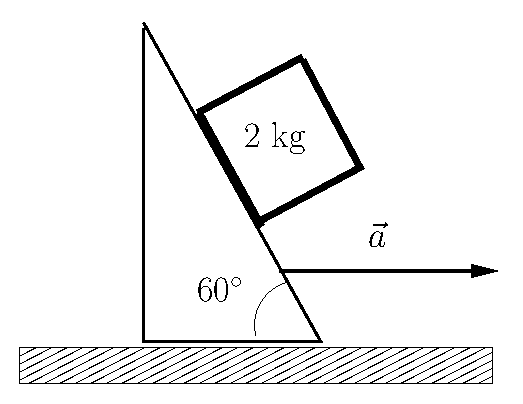
\includegraphics[width=2.5in]{additional_problems/wedge.eps}
    \end{center}
    \caption{Figure for Problem A\ref{prob:wedge}.}
    \label{fig:wedge}
  \end{figure}
  \begin{enumerate}
  \item What acceleration is required for this to occur?
  \item What would happen if the wedge were given an even greater
    acceleration?
  \end{enumerate}
  \label{prob:wedge}
\end{aproblem}
\vfill

\newpage
\begin{aproblem}{Using Forces to Predict Motion:  Dropping a Spring.}
  \begin{enumerate}
  \item Dangle your ``magic spring,'' holding it by one end, with the
    other end stretched out and hanging (relatively motionless) an
    inch or two above your other hand.  {\bf Don't do anything yet.}
    Think about what will happen when you let go of the top of the
    spring.

  \item {\em Before doing the experiment}, predict the order of the
    following five events.  Write down your prediction:. (i) The top
    end starts to move downward; (ii) The bottom end starts to move
    downward; (iii) The spring contracts halfway back to its
    unstretched size; (iv) The spring contracts all the way back to
    its unstretched size; (v) The bottom of the slinky hits your other
    hand.

  \item Now, once you have made your prediction, let go of the spring
    and see what actually happens.  You might have to do this a few
    times to figure out what the correct order is, or have a friend or
    two watch with you.  Write down the order of events as you
    actually observed them.

  \item Explain the results.  In doing so, you might want to draw a
    force diagram for the forces acting on the bottom loop of the
    spring both before and after the top of the spring is released.
    (Treat the bottom loop as a small mass hanging from the rest of
    the spring.)
  \end{enumerate}
\end{aproblem}

%\newpage

\begin{aproblem}{Force and Acceleration: Unwinding Yo-Yo.}
  \begin{enumerate}
  \item Wind up your yo-yo, and hold the end of the string (or put
    your finger through the loop).  Now, let the yo-yo fall out of
    your hand and unroll and drop downward (while holding the end of
    the string motionless).  Observe what happens.  Write down your
    observations.

  \item What can you say about the tension in the string while the
    yo-yo is unwinding?  Is the tension (i) equal to the weight of the
    yo-yo; (ii) less than the weight of the yo-yo but nonzero; 
    or (iii) zero?

  \item {\bf Explain} how you arrived at your answer.  You should be
    able to use the results of your observations, a force diagram and
    a simple use of Newton's 2$^{\rm nd}$ law to give a clear,
    definitive answer to the question. (We'll revisit this example
    again when we study rotations later in the semester.)

  \end{enumerate}
\label{prob:yoyoI}
\end{aproblem}


\begin{aproblem}{Circular Motion:  Around the World with Your Yo-Yo.}
  \begin{enumerate}
  \item Let the yo-yo hang at the end of the string and (holding the
    other end of the string) twirl it in a vertical circle so that it
    goes all the way around, being careful not to hit yourself or
    anyone around you in the head!  You should realize that you have
    to swing the yo-yo sufficiently fast; otherwise, it won't get all
    the way around.  Now, watch the string of the yo-yo as you swing
    it successively slower and slower until it falls out of the loop.

  \item Determine an expression for the theoretical minimum speed for
    the yo-yo at the top of its motion for it to complete the loop.
    Assume the string has a length $l$ and the yo-yo has a mass $m$
    and determine the minimum speed $v_{\rm top}$ as a function of
    $l$, $m$, and any fundamental constants.  \vspace{0.1in}

    {\bf Hints:} what happens to the string when the yo-yo is going
    just slightly too slow to be able to complete the loop?  What does
    this imply?  (The answer to this question is the key to solving
    this problem.)  Think back to Problem~A\ref{prob:return_ball}.
  \end{enumerate}
\end{aproblem}



%\parbox{4.6in}{
%\item {\bf Rough Ramp.}  Redo Tipler Chapter 4, problem 96, parts (a)
%and (b), but this time with friction.  Assume that the coefficient of
%kinetic friction between the $270\units{g}$ mass and the ramp is 
%$\mu_k = 0.1$.
%}

\begin{aproblem}{Friction Acting on Blow Dart.}
  \begin{enumerate}
  \item The goal of this exercise is to determine the average friction
    force acting on a blow dart as it slides across the floor.  Find a
    long, smooth, carpetless floor where you can fire a blow dart and
    watch it slide across the floor and eventually stop.  Smooth
    floors are the easiest surfaces to work with (the floors in Olin
    Science work well); for most other surfaces (e.g., carpeted
    floors), the dart will tend to bounce rather than slide.  You also
    might want to crouch down low and fire at a small, glancing angle.

  \item Determine the average friction force acting on the blow dart
    as it slows to a stop.  Make whatever measurements you deem
    relevant, and use the work-kinetic energy theorem --- this
    exercise is a snap if you do it this way, and a major pain if you
    try it any other way.  You can use your previous measurements of
    the initial speed of the blow dart once fired, and you might also
    be interested to know that the blow darts have a mass of $2.5\,
    \mbox{g}$ and a length of $6\units{cm}$, contain roughly
    $1.5\times 10^{24}$ protons and neutrons, and stick nicely to the
    front of your glasses.
  \end{enumerate}
\end{aproblem}

\newpage

\begin{aproblem}{Blow Dart Survivor.}
  \begin{enumerate}
  \item Let's say that you were stranded on a deserted island and a
    few dozen {\em Federal Express} boxes washed ashore.  Let's say
    further that one of the boxes contained a {\em Bandito Blow Gun}.
    In addition to being delighted at being able to complete your
    PHYS~211 homework, you also realized that you could replace the
    suction cups with pointed tips and use this to hunt the birds that
    flew overhead.  (You may neglect any effects of air resistance when 
    working this problem.)
  \item Use the Work-Kinetic Energy theorem along with results 
    of previous measurements to calculate how low a bird would have 
    to fly for you to have any chance of hitting it.
  \item Verify your results using the principle of conservation of
    mechanical energy.
  \item To test your prediction, fire a dart straight up into the air,
    just look at its path, and see if your result seems reasonable.
    You might even try firing it up near a tree or building whose
    height you know approximately.
  \end{enumerate}
\end{aproblem}

\begin{aproblem}{Losing Mechanical Energy: Superballs.}
  \begin{enumerate}
  \item Take one of your superballs and release it from rest above a
    hard surface such as your desk or uncarpeted floor.  {\bf
      Questions:} Does it bounce back up to the height you released it
    from?  Is its mechanical energy conserved?

  \item Estimate how much mechanical energy is lost in one bounce of
    the superball.  Make whatever measurements you deem relevant, and
    explain your process.  Some information that you may find helpful:
    the small and large superballs have masses 8.5 and $25\,
    \mbox{g}$, respectively.

%     \item  Now, repeat with your Glow-in-the-Dark Squishy Eyeball.
%     Where do you think the mechanical energy of the Eyeball has gone?
%     To enhance some effects (and to gross you out a little bit), try
%     throwing the Eyeball against the floor, a wall, or a window.
%     What are some of the forms of energy where the mechanical energy
%     of the superballs or the eyeball may have gone?
  \end{enumerate}
\end{aproblem}

\begin{aproblem}{Spring Forward. } 
  A woman of mass $m$ rides upward on a spring-loaded ejector pad of
  spring constant $k$.  It moves upward from rest through a distance
  $x_0$ at which point the spring potential energy is zero.  Right
  then the woman leaves the spring with speed $v$ and flies upward
  reaching a maximum height $h$ above her starting position.
  \begin{enumerate}
  \item Make a sketch showing her starting position, launch point, and
    maximum height.

  \item Write down an expression for the mechanical energy for each position.

  \item Equate these expressions to determine the woman's ejection
    speed and maximum height above her initial position in terms of
    $k$, $x_0$, and $m$.
  \end{enumerate}
  \label{prob:spring_forward}
\end{aproblem}


\begin{aproblem}{Extreme Skiing.}
  Lindsey Vonn has been challenged to test out a new ski event.  A
  loop of radius $R$ has been installed at the end of a ramp of height
  $h$ as shown in Fig.~\ref{fig:skiing}.  In this event the skier
  starts essentially from rest at the top of the ramp and gains 
  enough speed going down the ramp to complete a circle on the 
  inside of the loop.  You will need to use both force and energy methods 
  in this problem, and you may assume that the snow is frictionless.
  \begin{figure}[h]
    \begin{center}
    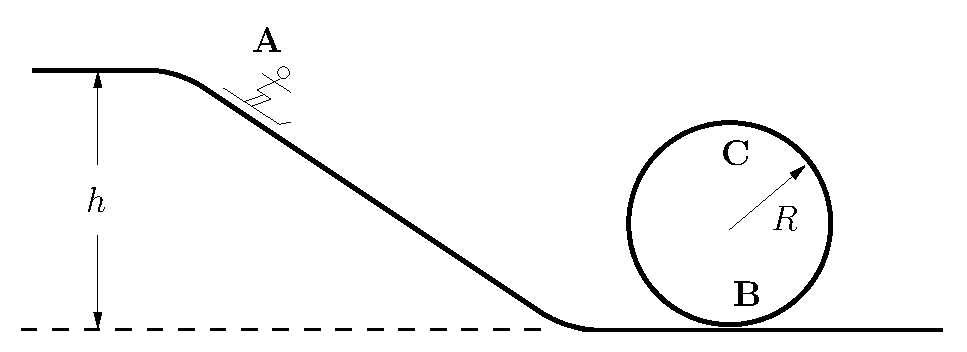
\includegraphics[width=4in]{additional_problems/skiing.eps}
    \end{center}
    \caption{Figure for Problem~A\ref{prob:skiing}.}
    \label{fig:skiing}
  \end{figure}

\begin{enumerate}
\item Draw a force diagram on Lindsey when she is as point {\bf A}.
Which statement about the magnitude of  
the normal force ({\bf N}) of the ramp on Lindsey at 
point {\bf A} is correct? 
\[ N = mg \hspace{0.3in}N < mg \hspace{0.3in} N > mg\hspace{0.3in}
N= 0\hspace{0.3in} \mbox{not enough info} \]
\item Draw a force diagram on Lindsey when she is as point {\bf B},
just {\em after\/} she has entered the circular loop.  Which 
statement about the magnitude of the normal 
force of the loop on Lindsey at {\bf B} is correct?
\[ N = mg \hspace{0.3in}N < mg \hspace{0.3in} N > mg\hspace{0.3in}
N= 0\hspace{0.3in} \mbox{not enough info} \]
\item Draw a force diagram on Lindsey when she is as point {\bf C}
at the top of the loop.  Which statement 
about the magnitude of the normal force of the loop 
on Lindsey at {\bf C} is correct?
\[ N = mg \hspace{0.3in}N < mg \hspace{0.3in} N > mg\hspace{0.3in}
N= 0\hspace{0.3in} \mbox{not enough info} \]
\item   Determine the minimum speed that Lindsey needs at point {\bf C} to 
stay on the track and make it around the loop.
\item Determine the minimum height $h$ in terms of the radius $R$
such that Lindsey can make it around the loop.  
\item What is the maximum magnitude of the force of the ground on 
Lindsey's skis for the minimum height, in  terms of her weight?
\end{enumerate}

%  \begin{enumerate}
%  \item  Where along the ramp and the loop is the magnitude of the force 
%  of the ground on the bottom of Lindsey's skis the greatest?
%
%  \item Determine the height $h$ in terms of the radius $R$ if the
%  maximum force of the ground on her skis is to be 4 times her weight.
%
%  \item With the height $h$ found in part (b), determine if she will
%    be able to make it completely around the loop.
%
%  \item Determine the minimum height $h$ in terms of the radius $R$
%    such that Lindsey can make it around the loop.  What is the maximum
%    magnitude of the force of the ground on her skis for this height, 
%    in terms of her weight?
%  \end{enumerate}
  \label{prob:skiing}
\end{aproblem}


\newpage
\begin{aproblem}{Trapped in Space.}  
  A spacecraft drifting through the center of a giant cosmic dust
  cloud experiences a potential energy that varies with position as
  shown in Fig.~\ref{fig:trapped} ($d$ is the distance from the center
  of the dust cloud).  The spacecraft starts at the center of the dust 
  cloud.   \begin{figure}[h]
    \begin{center}
    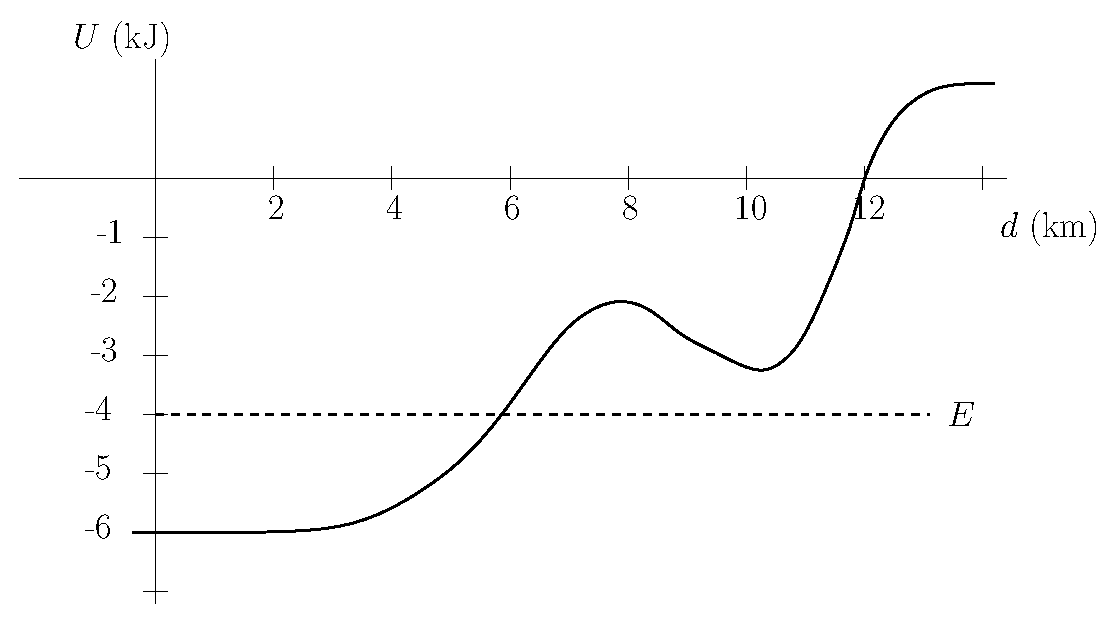
\includegraphics[width=4.5in]{additional_problems/trapped.eps}
    \end{center}
    \caption{Figure for Problem~A\ref{prob:trapped}.}
    \label{fig:trapped}
  \end{figure}
  \begin{enumerate}
  \item If the spacecraft has a total mechanical energy of $E = -4\units{kJ}$,
  what is the farthest distance it could drift from the cloud's center?
  \item Determine the kinetic energy of the craft when it is $2\units{km}$ 
  from the cloud center.
  \item Describe the motion of the spacecraft if it had started at the 
  center with a mechanical energy of $-2.5\units{kJ}$.
  \end{enumerate}
  \label{prob:trapped}
\end{aproblem}

\begin{aproblem}{Hopping Popper.}
  \begin{enumerate}
  \item In your kit, there should be a small rubber hemisphere that is
    referred to as a ``popper.''  If you turn it inside out and flex
    it for a few seconds, you can lay it on a table before it pops
    back into its original shape.  When it pops, it will jump up off
    the table, giving a nice demonstration of the conversion of
    potential energy into kinetic energy.

  \item Using whatever means you see fit, estimate the potential
    energy (in J) stored in the popper just before it pops.  (There's
    a really easy way to do this.)  The diameter of the popper is
    1~inch, its mass is $1.8\units{g}$, the hole in the center has a
    diameter of $2\units{mm}$, and there are approximately 3300
    students at Bucknell.
  \end{enumerate}
\end{aproblem}


\begin{aproblem}{Spring Slide Stop.}
  You push a block against a horizontal spring, compressing the spring
  by $15\units{cm}$.  When you release the block, the spring propels
  it across a level tabletop.  The block stops $75\units{cm}$ from
  its release point.  The spring constant is $200\units{N/m}$.
  Determine the magnitude of the friction force (assumed constant)
  between the block and the table.
\end{aproblem}



\begin{aproblem}{Superball Stack!}
  Take your larger superball and carefully balance your smaller
  superball on top of it.  Release both from rest, and allow them to
  fall perfectly vertically in a line.  The large superball should hit
  the ground first and then collide (going up) with the small
  superball (still on its way down).  This requires lots of patience
  and luck, but if you get it, the result is incredible!  This can be
  understood by treating the various collisions as perfectly elastic
  collisions, which they almost are.  
  %If you can manage to do this with
  %all three superballs, you are in for a real treat!
\end{aproblem}



\begin{aproblem}{Blow Darts and Superballs.}
  There is nothing that makes a day more complete than firing a blow
  dart at a small, defenseless superball.  Before doing this, though,
  here is some relevant information: the blow dart has a mass of
  $2.5\units{g}$ and the small and large superballs have masses 8.5
  and $25\units{g}$, respectively.
  \begin{enumerate}
  \item Now, put your larger superball (the bug or skull ball) at the
    edge of a table and softly fire a blow dart directly at it (do it
    until the blow dart hits almost straight on).  By ``softly'' we
    mean don't blow as hard as you usually do.  If you do this
    correctly, the dart should bounce straight back, and the large
    ball will move forward with only a very small speed.

  \item Now, the main question: What changes do you have to make such
    that the blow dart will continue forward after a head-on collision
    with another object?  Predict what you need to do, write down your
    prediction, and then test out your theory.
  \end{enumerate}
  \label{prob:blow_dart_superball}
\end{aproblem}

\begin{aproblem}{Hogwarts Hijinks.}
  Harry and Hermione are playing in the GraviFree Room at Hogwarts.
  Harry (mass $55\units{kg}$) is floating motionless in the center
  of the room.  Hermione (mass $45\units{kg}$) pushes off from the
  wall and approaches Harry at a speed of $6.0\units{m/s}$.  Neglect
  air resistance in this problem.
  \begin{enumerate}
  \item As Hermione moves past Harry, he reaches out and grabs her
    outstretched hand, holding on tightly.  Determine the speed with
    which Hermione and Harry move after they grab hold of each other.
 
  \item Harry and Hermione notice Ron giving them a funny look, so
    they let go of each other.  Determine the speed with which
    Hermione moves after they let go.

  \item Determine the speed with which Harry moves after they let go.
     
  \end{enumerate}
  \label{prob:hogwarts}
\end{aproblem}


\begin{aproblem}{Railing in the Rain.}
  An open railroad car of mass $2\times 10^4\units{kg}$ is rolling
  without friction along a level track at $5\units{m/s}$ when it
  starts to rain.  After the car has collected $2000\units{kg}$ of
  water, it stops raining.  Assume that the rain fell perfectly
  vertically.
  \begin{enumerate}
  \item What is the rail-car's speed after it stops raining?

  \item After the rain has stopped, a hole in the bottom of the
    rail-car is unplugged, and the rain water begins to leak out of
    the hole at a rate of $5\units{kg/s}$.  What is the speed of the
    rail-car after half the rain water has leaked out?

  \item What is the speed after all the rain water has leaked out?
  \end{enumerate}
\end{aproblem}


\begin{aproblem}{Relative Velocities (Classical).}  
  A typical person walks with a speed of about $2\units{m/s}$
  relative to the ground.  While you are walking between classes,
  watch other students who happen to be walking in the same and
  opposite direction as you, and answer the questions in the following
  parts.
  \begin{enumerate}
  \item Choose a student walking in the same direction as you with the
    same approximate speed.  Note how far away that person is from
    you.  Then, after the two of you have walked for a few seconds,
    note again how far that person is from you.  Has the distance
    between the two of you increased, decreased or stayed roughly the
    same?  Assuming that you are both walking at a speed of $2\,
    \mbox{m/s}$ relative to the ground, what does your previous answer
    imply about the speed of the other person as measured in your
    reference frame?

  \item Do the same thing for a student walking in the opposite
    direction as you.  Answer the same questions as in part a).

  \item If you happen to see someone running to class, but going in
    the same direction as you, ask yourself the same questions as in
    part a).
  \end{enumerate}
\end{aproblem}

\begin{aproblem}{Measuring the Length of a Moving Object, Take 1.}
  Measuring the length of an object that is at rest with respect to
  you is pretty easy: one method is to take a ruler of some kind, hold
  it up to the object, and note where each end of the object is with
  respect to the ruler.
  \begin{enumerate}
  \item What difficulties arise if you try to measure the length of an
    object that is moving with respect to you using the technique
    described above? 

  \item Other methods need to be developed to measure the length of a
    moving object.  We'll have you try an approach that employs a
    group of people.  [We will do the following as a class exercise
    during problem session, so you won't have to gather a group of
    your own.]  Go outside, and line up in a row, parallel to a street
    with some automobile traffic.  (Please stand a safe distance away
    from the street!).  Stand so that there is approximately equal
    distance between you and your nearest neighbors \medskip

  \item Your instructor will stand across the street.  When a car
    comes by, your instructor will yell ``Now!''.  If the front of the
    car is directly in front of you, {\bf raise your hand} and {\bf
      keep it raised}.  If the back of the car is directly in front of
    you, {\bf raise your hand} and {\bf keep it raised.}  (By yelling
    ``Now!'' your instructor has basically synchronized your clocks,
    so that you are making your measurements --- i.e., raising your
    hand --- simultaneously.  You'll see in Problem
    A\ref{prob:synchronizeA} that to make this measurement even more
    carefully, we would have to come up with a better method of
    synchronization.  We'll discuss some thorny issues involving
    simultaneity in an upcoming lecture.)  \medskip

  \item Now, measure the distance between people who have their hand
    raised.  How is this distance related to the length of the car?
    Does it matter how fast the car is going in using this technique?
  \end{enumerate}
  \label{prob:moving_objI}
\end{aproblem}

\begin{aproblem}{Measuring the Length of a Moving Object, Take 2.}
  In problem A\ref{prob:moving_objI} you measured the length of a
  moving object using several people and synchronization.  In this
  problem, you will develop a technique that you could use on your
  own.
  \begin{enumerate}
  \item Assume that you know the velocity of the car (say the car is
    going the speed limit), and that your available tools are a ruler
    and a clock.  Figure out a method to determine the length of the
    moving car.  Describe what you would do and what you would
    measure. and how you would use the results of your measurement to
    determine the length.

  \item You likely measured a time interval and/or a distance.  Think
    how the driver of the car views the situation, especially if the
    speed were relativistic (say if the car were going at $0.8c$
    relative to you).  Would the driver of the car agree with your
    measurement of the time interval and/or distance?  Would she think
    your measurements are too high?  too low?  correct?

  \end{enumerate}
\end{aproblem}

\newpage

\begin{aproblem}{Synchronization, Simultaneity and Spacetime Diagrams.}
  \begin{enumerate}
  \item Grab a friend or roommate (it doesn't have to be someone
    taking PHYS 211).  Stand on opposite sides of a room or a long
    hallway (the larger the separation distance, the better).  Throw a
    ball to your friend (or have that person throw the ball to you).
    Draw a qualitative spacetime diagram of this situation, showing
    world lines for you, your friend, and the ball.

  \item Your next goal is to have both of you clap your hands at
    precisely the same time, but you have to keep your eyes closed
    while doing it.  Here's an approach that you might try: you could
    say (loudly), ``On the count of three, we'll both clap our hands.
    One, two, THREE!''  Go ahead and try this, and then comment on
    inaccuracies in this method (i.e., why doesn't this work?).  Draw
    a spacetime diagram to support the argument.

  \item See if you can figure out a way that will result in you and
    your friend clapping at the same time.  Write down the method, and
    draw a spacetime diagram that demonstrates that this is a good
    approach.
  \end{enumerate}
\label{prob:synchronizeA}
\end{aproblem}


\begin{aproblem}{Life in a Relativistic World, Part I.}
  A typical person walks with a speed of about $3\units{mph}$
  relative to the ground.  For this problem, imagine that the speed of
  light were actually $4\units{mph}$ rather than $3.0\times 10^8\units{m/s}$.

  Walk across campus, perhaps on your way to or from class or going to
  dinner.  Choose a time when there is a lot of activity around you
  (cars moving around, other people walking around, etc).  While you
  are walking, watch everything around you.  Note what you see, what
  you feel, whatever you experience (when you are moving, waiting to
  cross a street, etc.), and think about how any of these things would
  be different if the speed of light were $4\units{mph}$.  {\bf
    Write a couple of paragraphs summarizing your thoughts.}  And feel
  free to discuss this with other people in the class.  (Some things
  to think about in particular: length contraction, time dilation, and
  simultaneity --- all of these things would be {\em very} noticeable
  in this hypothetical scenario.)

  If you really think about a lot of the things around, you should
  come to the conclusion that if $c$ were really $4\units{mph}$, it
  would truly be a whacked-out, psychedelic,
  something-out-of-a-Salvador-Dali-painting experience.
  \label{prob:rel_worldI}
\end{aproblem}


\begin{aproblem}{The Real Potential of a Superball.}  
  Pick up your largest superball and just stare at it for a little
  while.  Does this look like it contains a lot of energy?  Now,
  estimate its mass (or alternately look back at the Problem
  A\ref{prob:blow_dart_superball} where the mass is given) and
  determine the rest energy of the superball (in Joules).  Now,
  consider that an atomic bomb releases $10^{14}$ to
  $10^{15}\units{J}$ of energy; consider also that a typical household
  uses about $10^{10}\units{J}$ of energy per year.  Stare at your
  little ball again.  Write a sentence or two about your thoughts.
  (Feel free to post your thoughts on the ``Questions'' page at the
  course web-site if you want to share them.)
\end{aproblem}

\begin{aproblem}{Life in a Relativistic World, Part II.}  
  Let's think a little more about what it would be like walking across
  campus if the speed of light were $4\units{mph}$ rather than
  $3\times 10^8\units{m/s}$.  You've already thought about time
  dilation, length contraction and simultaneity in problem
  A\ref{prob:rel_worldI}.  Now, think about what the relationship $E =
  mc^2/\sqrt{1-v^2/c^2}$ would mean in a relativistic world.
  \begin{enumerate}
  \item If the speed of light were $4\units{mph}$, how much {\em
      kinetic} energy would be involved in walking at a speed of
    $3.5\units{mph}$?  (Use your own body mass in these estimates.)
    How much kinetic energy would you have walking at $3.8\,
    \mbox{mph}$?  How do you think you would feel as you start trying
    to walk faster and faster, past $3.0\units{mph}$, past $3.5\,
    \mbox{mph}$, past $3.8\units{mph}$, past $3.9\units{mph}$,
    \dots ?

  \item What do you think might happen if you collided with another
    person if you were both walking with a speed of $3.8\units{mph}$
    but in opposite directions?
  \end{enumerate}
\end{aproblem}

\begin{aproblem}{Life in a Really Relativistic World.} 
  Common misconceptions about relativity abound.  You'll hear people
  say that relativity states that ``if you are on a ship traveling
  close to the speed of light, your mass increases to infinity, you
  shrink down to zero size, and you never age.''  Statements like this
  have led people to think that life would be very strange on such a
  spaceship.  We want you to experience what it really would be like
  to be on such a spaceship. 

  So, go ahead and do this experiment.  Hop on a spaceship that is
  traveling at a speed of at least $0.8c$ relative to some reference
  frame.  Before you start saying that we've completely cracked up,
  there is a spaceship that everyone in this class has access to that
  meets this requirement.  (Hint: the name of the ship starts with the
  letter $E$ and its name rhymes with {\em birth}, and it is currently
  traveling at a speeds of greater than $0.9c$ relative to distant
  galaxies and quasars.) 

  {\bf Question:} Do you feel at all strange being on such a ship?
  Write a sentence or two of your thoughts about this.  (Feel free to
  post your thoughts on the ``Questions'' page at the course web-site
  if you want to share them.)
\end{aproblem}

\newpage
\begin{aproblem}{Photon Absorption} 
  An elementary particle has a rest mass of \break $1125\units{MeV/$c^2$}$,
  and is motionless in some reference frame.  A photon with momentum
  $750\units{MeV/$c$}$ strikes the particle and is absorbed, leaving
  an ``excited'' particle that is recoiling and nothing else.
  Determine the mass and recoil velocity of the excited particle after
  the interaction.
  \label{prob:photon_absorption}
\end{aproblem}

\begin{aproblem}{Let There Be Light.}  
  Particle A of mass $400\units{MeV/$c^2$}$ collides with the
  stationary particle B of mass $350\units{MeV/$c^2$}$.  The result of
  this collision is a single particle C at rest, and a
  $300\units{MeV}$ photon.  Determine the mass of particle C.
  \label{prob:light}
\end{aproblem}


\begin{aproblem}{What's That Skull (or Bug) Doing in My Superball? }
  We can take advantage of the poor bugs and skulls trapped in your
  larger superball to comment on the rotation of the ball.
  \begin{enumerate}
  \item Take your superball and rotate it slowly, watching the object
    as it rotates.  You can either do this in your hand, or toss it
    gently with a little rotation --- whichever enables you to see the
    object spinning easiest.  Try rotating it quickly as well.  What
    can you say about the motion of the middle portion of the object,
    as opposed to the motion of the part of the object farthest from
    the middle?  How does your answer to the previous question relate
    to the equation $v = r\omega$ for tangential speed?

  \item Now, drop the superball straight down while spinning it very
    rapidly about a horizontal axis.  The best way to do this is to 
    use two hands to get it
    spinning as fast as you can while releasing the ball.  What
    happens when the ball bounces?  Specifically, does it bounce
    straight up?  Why not?  (You'll want to use a diagram and Newton's
    $2^{\rm nd}$ and $3^{\rm rd}$ laws to support your argument.)
    Also, what happens to the angular velocity of the superball after
    it bounces?  Explain {\em why} this happens.  (Consider the torque
    acting on the ball when it bounces on the floor.)

  \item (Optional) If you are good at spinning the ball, try this:
    toss the ball slightly away from you, but spinning with the top
    toward you.  If you do this well, you can get the ball to bounce
    back and forth on the ground.  Explain {\em why} this happens.

  \end{enumerate}
\end{aproblem}

\begin{aproblem}{Yo-yos (revisited) with Rotations.}
  We're going to repeat Problem A\ref{prob:yoyoI}, but this time we're
  going to be quantitative and take rotation into account.
  \begin{enumerate}
  \item Count how many turns of the string are required to wind up the
    yo-yo all the way.  From this, calculate $\Delta\theta$ for the
    yo-yo to unwind completely (in radians).  Now, holding the end of
    the string, let the yo-yo unwind all the way, and estimate the
    time for it to reach the bottom (within a couple of tenths of a
    second). Since the angular acceleration is constant during this
    process, you should be able to take two integrals of $\alpha$ to
    find that $\Delta\theta = \alpha t^2/2$.  From this information,
    determine the angular acceleration of the yo-yo as it falls.

  \item Now estimate the average radius of the spool (i.e., the
    average distance of the point-of-contact of the string from the
    center of the yo-yo), and use this information to estimate the
    linear acceleration of the yo-yo during its fall.  Then, use this
    information (along with a force diagram and Newton's second law)
    to determine the tension in the string while the yo-yo is falling.
    Note: the mass of the yo-yo is $52\units{g}$, its total
    thickness is $3.5\units{cm}$, and it fits nicely in your pocket.

  \item Is your result from part (b) for the tension consistent with
    the qualitative answer from Problem~ A\ref{prob:yoyoI}?

  \end{enumerate}
\end{aproblem}

\begin{aproblem}{As the Ball Turns.}
  A solid $1.4\units{kg}$ ball with diameter $15\units{cm}$
  rotates about its diameter at 70 revolutions per minute.
  \begin{enumerate}
  \item Determine the kinetic energy of the solid ball.
  \item If the ball had the same mass and diameter, but all the mass
    was at the outer surface of the ball (in other words, the ball
    were hollow), would the ball have more or less kinetic energy than
    you calculated in part a)?  Assume this hollow ball has the same
    angular speed.
  \item Back to the solid ball again.  If you add an additional $2\,
    \mbox{J}$ of rotational kinetic energy, determine the solid ball's
    new angular speed.
  \end{enumerate}
  \label{prob:ball_turns}
\end{aproblem}

\begin{aproblem}{Yo-yos, mechanical energy, and angular momentum.}
  \begin{enumerate}
  \item Unwind the yo-yo and rotate it in a vertical circle at the end
    of its string.  Once it is going, allow the yo-yo string to wrap
    around your arm --- the result should be that the yo-yo spirals
    inward until all the string is wrapped around your arm.  Do this a
    few times and watch the yo-yo as it spirals inward.  Do you think
    the yo-yo is speeding up, slowing down, or going at basically the
    same speed during this process?  (Watch the yo-yo very carefully
    here --- your eyes can easily trick you.)

  \item Now, think about this process both from a perspective of
    mechanical energy and angular momentum.  Which of these quantities
    do you think are conserved during this process (or do you think
    that neither or both are conserved)?  Justify your answers: for
    angular momentum, you'll need to show either that torque acting on
    the yo-yo is zero or non-zero, and for energy, you'll need to
    explain either that work is or is not being done on the yo-yo.
    Based on these answers, should the yo-yo be speeding up, slowing
    down or basically going at the same speed while spiraling inward?

  \item Now do the same thing again, but this time, instead of letting
    the string wind around your arm, thread the string through a PVC
    tube (which we'll provide in problem session) and pull the string
    through the tube to pull the yo-yo inward.  Answer all the same
    questions that you did in parts a) and b).
  \end{enumerate}
\end{aproblem}

\begin{aproblem}{Yo-yos and torque.}
  \begin{enumerate}
  \item Take a partially-wound (i.e., partially-unwound) yo-yo and
    place it on a level surface such that it could roll if pushed or
    pulled.  Now, predict which way it will roll if you pull the
    string straight up.  (Justify your prediction with diagrams.)
    Try the experiment --- were you correct?  If
    not, justify what actually happened.

  \item Now, do this again, but this time let the string go over the
    top of the yo-yo and pull it parallel to the table.  Again, first
    make a prediction about which direction the yo-yo will move (and
    justify it), then try the experiment.  Again, if you were not
    correct in your prediction, justify what actually happened with
    diagrams and Newton's laws.

  \item Finally, predict which way the yo-yo will move if the string
    goes underneath the yo-yo, and you pull it parallel to the table.
    (Again, justify your prediction with a diagram. 
    Try the experiment.  Were you
    correct?  Again, if you were not, then justify what you actually
    saw.
  \end{enumerate}
\end{aproblem}
\newpage

\begin{aproblem}{When Wheels Collide.}  
  Two solid wheels of identical mass but different radii ($R$ and
  $2R$) are spinning on the same axle (on very smooth bearings).  The
  wheels are spinning in opposite directions, but with the same
  angular speed $\omega_i$, as shown in Fig.~\ref{fig:wheels}.  The
  two wheels are slowly brought together, and the resulting frictional
  interaction between the touching surfaces eventually brings the
  wheels to a common angular speed $\omega_f$.
  \begin{figure}[h]
    \begin{center}
    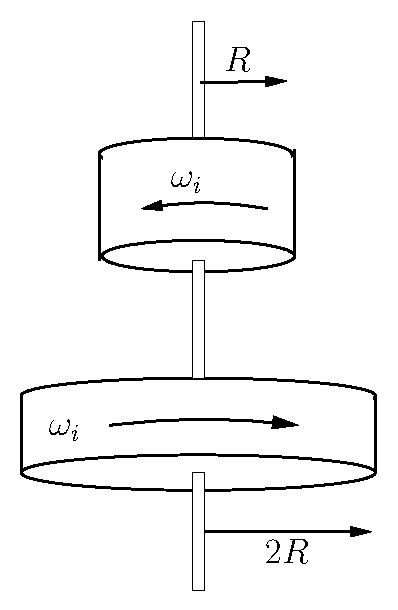
\includegraphics[width=1.5in]{additional_problems/wheels.eps}
    \end{center}
    \caption{Figure for Problem A\ref{prob:wheels}.}
    \label{fig:wheels}
  \end{figure}
  \begin{enumerate}
  \item Determine $\omega_f$ in terms of $\omega_i$.
  \item Are the wheels now rotating in the original rotation direction
    of the larger or the smaller wheel?
  \end{enumerate}
  \label{prob:wheels}
\end{aproblem}



\begin{aproblem}{How much do you suck?}
  \begin{enumerate}
  \item In problem session, you will be provided with a container that
    can hold water and a piece of flexible tubing.  Fill the container
    with some water and place the container on the floor.  Take your
    piece of flexible tubing and put one end into the water and stand
    up with the other end.  Put the other end into your mouth and
    breath in, pulling the water up the tube.  Don't breath in the
    water --- that wouldn't be very fun. (That shouldn't be a problem
    because if you are standing up, you won't be able to get the water
    all the way up the tube anyway.)  Estimate the maximum height
    above the water surface that you can hold the water by continually
    breathing inward.  {\bf Important:} don't use your cheeks to suck
    on the tube.

  \item Now, use this height to determine the ``gauge pressure'' of
    your lungs when you suck (the difference between your lungs'
    pressure and atmospheric pressure).  To do this, determine the
    force required to hold up a column of water with height $h$ in a
    tube with cross-sectional area $A$ (keep things in variables ---
    don't put the numbers in yet).  Once you have the force, you
    should be able to get the gauge pressure ($\Delta p$) from the
    relation between force, pressure and area.  Then, put the numbers
    in.  What is the {\em absolute} pressure that your lungs achieve
    when you suck?

  \item If you could make a perfect vacuum with your lungs, what would
    be the maximum height that you could suck water up in a straw?

  \item Now, let's see how hard you can blow.  Fill up the tubing
    about 2/3 to 3/4 of the way with water.  The easiest way to do
    this is to bend down low and suck water again. (Do you notice how
    much easier it is to suck up the water when it doesn't have to
    climb as high?).  A little before the water reaches your mouth,
    stop sucking and lift up the two ends of the tubing to make a
    ``U'' shape.  Now, blow into one end while raising the opposite
    end.  If you have a friend to help, that would be good --- he/she
    can continually raise the other end to make sure that you don't
    blow the water out of the tubing.  Estimate the maximum height
    (above your mouth) that you can hold the water, and use this
    information to estimate the gauge pressure and absolute pressure
    of your lungs when you are blowing.

    {\bf Note:} What you have just done is a technique that is used
    all the time in the medical industry to measure lung performance
    in patients.  This is particularly useful for patients with lung
    cancer or various breathing disorders --- this kind of test can
    quickly and easily determine how well the lungs are functioning.

  \item If you made a straw several hundred miles long, stuck one end
    into the ocean and stuck the other end out into the vacuum of
    space, would the straw suck up all of the ocean water into space?
    Why not?  (In fact, the water wouldn't rise up at all in the tube.
    Try to figure out why it wouldn't.)
  \end{enumerate}
  \label{prob:suck}
\end{aproblem}


\begin{aproblem}{Dunking Birds and the Ideal Gas Law.}
  \begin{enumerate}
  \item We're not actually going to use the dunking bird in its
    intended purpose here (don't worry --- that will come).  Instead,
    grab the Bird's bottom in the palm of your hand and wrap your hand
    around it.  Presumably, if your hand is at normal body temperature
    (37$^\circ$~C), the fluid in the Bird will rise up toward the
    head, leaving a larger volume of gas than when you started.

  \item Estimate the volume of the gas in the Bird's bottom before and
    after you warmed it up with your hand.  Actually, you really only
    need to approximate the ratio of the two volumes 
    $V_{\rm after}/V_{\rm before}$.  Now, determine the ratio of the 
    temperature of your hand to the temperature of the air, using estimates 
    of the room temperature and your body temperature.  (What
    units are you using for temperature?)  Using the ideal gas law,
    determine if the change in the volume is consistent with the
    change in the temperature.  (Show all your work here.)

  \item What else do you think is going on inside the Bird?  We're not
    expecting a complete answer --- this is more of a set-up to help
    motivate the next class.  But you should be able to use the ideal
    gas law to make some statements about what else is going on inside
    the Bird.
  \end{enumerate}
  \label{prob:birdI}
\end{aproblem}

\begin{aproblem}{Pressure and Force.} 
  It is fairly straightforward to estimate the pressure inside a blow
  dart's suction cup when it is sticking to something.  First, we'll
  look at it qualitatively, then put some numbers in.
  \begin{enumerate}
  \item Wet the suction cup on one of your darts and press it onto a
    flat, smooth surface so that it sticks.  (It's best to have the
    dart wet, because this will keep air from leaking in around the
    suction cup.)  Pull on the dart and note how much force is
    necessary to pull the dart off the surface.  You don't have to be
    quantitative here; simply comment on how difficult it is to pull
    off.

  \item While you are pulling on the dart, what is causing the force
    that pulls (pushes) the dart {\em back onto the surface}?  Of
    course, this is due to the pressure difference between the inside
    and the outside of the suction cup, but what {\em physically} is
    causing the force?  (Refer to the kinetic theory of gases to
    answer this.)

  \item Now, let's do this semi-quantitatively.  If you stuck the dart
    to the underside of a smooth surface, you could hang about $1\,
    \mbox{kg}$ of mass from the dart without it coming off.  Based on
    this, you can determine the maximum force (in N) that the dart can
    withstand before coming off the surface.  And once you have the
    maximum weight that it can hold, use the definition of pressure
    (in terms of force and area) to estimate the pressure within the
    suction cup.  Note: the suction cup has a diameter of about $1.8\,
    \mbox{cm}$.  (You should estimate the pressure {\em difference}
    between the air and the inside of the cup first, then you can get
    the absolute pressure inside the cup.)

  \item If there were a perfect vacuum inside the suction cup, what
    would be the maximum weight that it could hold?
  \end{enumerate}
\end{aproblem}


\newpage
\begin{aproblem}{Balloons and Bottles.}
  \begin{enumerate}

  \item Do the following experiment: Get a glass drink container ---
    one of those juice/cranberry bottles will work, but a
    taller/deeper glass drink container is better.  (You might be able
    to pluck something out of one of the recycling bins if needed.)
    You'll need to stretch a balloon across the opening of the jar, so
    try that out to make sure you can do it, then take the balloon
    off.  Then, boil a small amount of water (you can use a microwave
    if you want, but make sure that the water is really hot and
    steaming).  Pour a small amount of the boiling water into the jar
    (cover only the bottom cm or so).  If the water is hot enough,
    there should be a noticeable amount of steam coming out of it.
    Then, stretch the balloon over the mouth of the jar and then watch
    the system as things slowly cool down.

  \item Describe what happens, and explain {\em why} it happens.  In
    particular, comment on any condensation of the steam that you see
    on the inside of the container.  Is this condensation important as
    far as the behavior of the balloon is concerned?

  \end{enumerate}
\end{aproblem}


\begin{aproblem}{Using Phase Transitions to Cool a Drink.}  
  You'll need to do this at lunch or dinner, or somewhere that you
  have access to ice.
  \begin{enumerate}
  \item Get three glasses or cups.  Fill one glass (let's call it
    glass A) with a mixture of ice and water (plenty of ice), and fill
    the other two glasses each halfway full with room temperature
    water.  Let the ice/water mixture in glass A sit for a few
    minutes: this will ensure that both the ice and the water in the
    glass are at temperature 0$^\circ$~C.

    Next, you are going to take out a fair amount of $0^\circ$~C ice
    from glass A (a spoon is a convenient way to do this) and dump it
    into glass B, one of the half-filled room-temperature glasses.
    Then pour an equivalent amount of $0^\circ$~C water from glass A
    into glass C, the other half-filled glass.  The idea is to compare
    the cooling effects of $0^\circ$~C ice compared to $0^\circ$~C
    water.

    Before doing the experiment {\bf predict} whether glass B and
    glass C should be equally cooled, or if not, which will be cooler.
    Write down your prediction.

  \item Now, go ahead and do the {\bf experiment}.  Record the results
    in your notes.  Is the result what you expected?  Use heat flow
    arguments to {\bf explain} why you obtained this result.

  \end{enumerate}

%This experiment should begin to convince you that you can cool a drink
%much more with an ice cube at $0^\circ\units{C}$ than with an equal
%amount of $0^\circ\units{C}$ water.  The idea of using phase
%transitions in cooling applications is very widespread; in fact,
%commercial air conditioners depend on some sort of fluid (like freon)
%that vaporizes easily (i.e. changes phase) to absorb the heat from the
%object or area that is being cooled.  
\end{aproblem}


\begin{aproblem}{The Dunking Bird, revisited.} 
  In Problem A\ref{prob:birdI}, you should have found that the
  temperature change alone wasn't enough to cause the volume change
  and the resulting movement of the fluid up into the Bird's head ---
  there must have been a significant change in $N$, the number of gas
  molecules in the Bird.

  \begin{enumerate}
  \item Explain how $N$ is increasing in the Bird's bottom when you heat
    it with your hand.  Explain also how $N$ decreases in the head
    when the head is cooled.  What about the fluid inside the Bird ---
    why do you think the Dunking Bird is filled with methylene
    chloride instead of simply dyed water?

  \item Now, how is the head of the Bird cooled during its normal
    dunking operation?  Does the water in the glass have to be cooler
    than the room temperature?  Try the following experiment: try
    using water in the glass that is measured to be the same as room
    temperature or better yet, heat up the water to be several degrees
    above room temperature, and dip the Bird's head in this warm
    water.  {\bf Question:} does the Bird still dunk?  (The result
    might surprise you.)  So, how {\em does} the Bird's head cool?

  \item A Dunking Bird with a wet head is comparable in many respects
    to a person who is sweating on a hot day.  Based on what you know
    about phase transitions (melting, vaporization, etc.), explain
    {\em why} it is necessary for a person to sweat on a hot day.  Why
    doesn't a person sweat as much on cooler days?
  \end{enumerate}
\end{aproblem}


\begin{aproblem}{Energy Stored in a Balloon.}
  \begin{enumerate}
  \item When you blow up a balloon, you are clearly doing work on the
    balloon.  Alternatively, you can say that the gas in the expanding
    balloon is doing work.  And this work goes into potential energy.
    {\bf Question:} where is that energy ``stored''?

  \item In this problem, we're going to estimate that stored energy
    using $W = \int p\, dV$.  We'll use the approximation that the
    pressure is almost constant (we'll estimate an average pressure)
    so that $W= p\, \Delta V$.  And since the air outside the balloon
    is doing negative work on the balloon while it expands, and we
    want the {\em net} work done by the gas, you can use the gauge
    pressure to get the net work done by the air while the balloon
    expands.

    To estimate the gauge pressure, you need to attach the balloon to
    the end of your flexible hose with a rubber band, blow the balloon
    up half-way, then make sure to pinch off that end of the balloon.
    Now, get some water into the tube (still holding the balloon end
    pinched off), and then hold up the tube (in a U-shape, with the
    balloon at one end and the open end of the tube at the other).
    Finally, release the balloon such that the gauge pressure of the
    balloon pushes the water in the tube.

  \item Use this technique to estimate the average gauge pressure (see
    problem A\ref{prob:suck} for a refresher if you have forgotten),
    and estimate the change in volume when the balloon is fully
    inflated.  From this, you should be able to estimate the energy
    stored in the balloon.
  \end{enumerate}
\end{aproblem}



\begin{aproblem}{The Thermodynamics of Blow Darts.}  
  Let's think about what happens when you fire a blow dart.  We'll use
  the results from problem A\ref{prob:suck} (in which you determined
  the gauge pressure that your lungs can produce) to estimate the
  ideal maximum speed that you could achieve when firing a blow dart.

  \begin{enumerate}

  \item When you blow on the dart, the pressure $p_{\rm lung}$ from
    your lungs pushes the dart down the tube while atmospheric
    pressure $p_0$ pushes the dart the other way.  Draw a quick sketch
    of the dart, and draw arrows corresponding to the forces $F_{\rm
      lung}$ and $F_{\rm atm}$ on the dart.  Considering that the dart
    has a cross-sectional area $A$, what is the net force acting on
    the dart when you fire?  Re-write this result in terms of the
    gauge pressure for your lungs.

  \item Now, use the result from A\ref{prob:suck} and the fact that
    the dart has a diameter of about $1.8\units{cm}$ to estimate the
    net force acting on the dart when you blow.  Now, considering that
    the active part of the blow gun is about $50\units{cm}$ long,
    estimate the work done on the dart when firing.  (Note: you'd get
    the same result by using $W = P_{\rm gauge}\, \Delta V$.)
    Finally, use the work to predict the exit speed for the dart when
    you fire.

  \item The answer that you get here might differ significantly from
    what you measured in Problem~A\ref{prob:dartI}.  Why do you
    suppose these two results could be so different?  Do {\bf not} use
    ``human error'' anywhere in your response!
  \end{enumerate}
\end{aproblem}

\begin{aproblem}{Path Matters.} 
  One mole of an ideal monatomic gas is heated from $300\units{K}$
  to $600\units{K}$.
  \begin{enumerate}
  \item If the gas is held at constant volume, find the change in the
    gas's internal energy, the work done by the gas, and the heat
    added to the gas during this process.

  \item If the gas is held at constant pressure, find the change in
    the gas's internal energy, the work done by the gas, and the heat
    added to the gas during this process.
  \end{enumerate}
\end{aproblem}

\newpage
\begin{aproblem}{Some Cycle.} 
  In the cycle shown below, $1.0$ mole of a
  monatomic ideal gas is initially at a pressure of $p_A=100\units{kPa}$
  and a temperature of $T_A=0^\circ\units{C}$.  The gas is heated at
  constant volume to $T_B = 150^\circ\units{C}$ and is then expanded
  adiabatically until its pressure is back to $p_C=100\units{kPa}$.
  Finally, the gas is compressed at constant pressure until it is back
  to its original state $A$.  Find

  \begin{enumerate}
  \item the temperature $T_C$ after the adiabatic expansion,
  \item the heat entering or leaving the system during each process,
  \item the efficiency of this cycle, and
  \item the efficiency of a Carnot cycle operating between the
    temperature extremes of this cycle.
  \end{enumerate}
  \begin{figure}[h]
    \begin{center}
      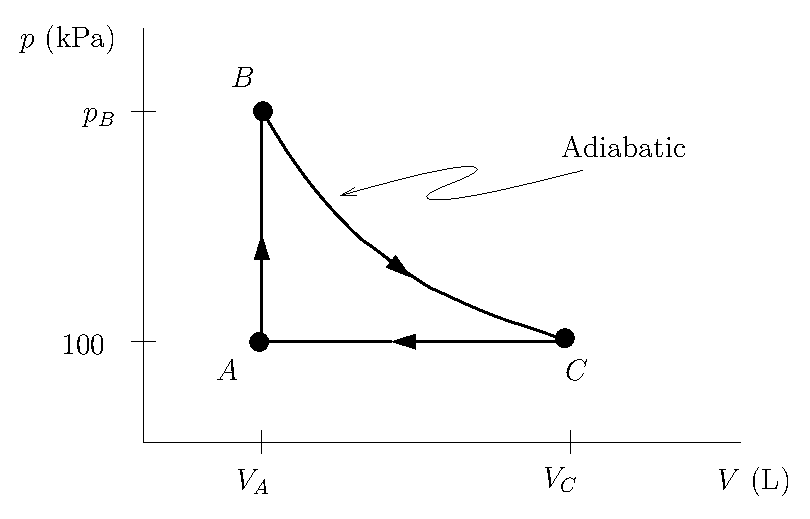
\includegraphics[width=4in]{additional_problems/cycle.eps}
    \end{center}
    \caption{Figure for Problem A\ref{prob:cycle}.}
    \label{fig:cycle}
  \end{figure}
  \label{prob:cycle}
\end{aproblem}
\newpage


\begin{aproblem}{Dunking Birds as Heat Engines.} 
  First, get your Dunking Bird going.  You can actually operate it one
  of two different ways:
  \begin{itemize}
  \item[(I)] You can get the head wet and then just put it on a table.
    If the Bird is properly balanced (you may have to slide the metal
    piece up or down), then it should start going.

  \item[(II)] You could place the Bird on top of a TV or computer
    monitor and let the heat from that device warm the Bird's bottom.
    ({\bf Warning:} Be careful if you do it this way: people have
    wound up with blue or red stained monitors and desks as well as
    having to clean up broken glass!)
  \end{itemize}


  \begin{enumerate}
  \item If the Dunking Bird is being powered by heating of its bottom 
    (i.e., Method II above), the gas/fluid in the bottom will undergo
    several steps.  (The steps are actually continuous, but we'll
    break them up to make this easier to plot.)  (i) As the bottom heats
    up, the pressure of the gas inside increases.  (Do you remember
    why?  It isn't just the change in temperature.) (ii) After the
    pressure has increased, the fluid is forced out of the bottom, and
    the volume of gas in the bottom increases.  (iii) The Bird tips over
    and the air in the bottom and the air in the head are connected,
    causing a quick drop in the pressure of the gas in the bottom down
    to its initial value.  (iv) The Bird stands up again, and the
    fluid runs down into the bottom, decreasing the volume of gas in
    there.

    Plot the sequence described above on a $P$-$V$ diagram.  Do you
    have a cyclic process here?  Show the work for the engine cycle on
    your $P$-$V$ diagram.

  \item Repeat part (a), but for Method I (where the Bird's head is
    cooled by evaporation).

  \item What is the hot reservoir for this engine?  What is the cold
    reservoir?  What is the work done by the Bird (in words)?  Draw an
    engine diagram for the Bird.
 
  \end{enumerate}
\end{aproblem}


\begin{aproblem}{Entropy and the Second Law.}
   \begin{enumerate}
   \item Scatter at least 10 coins over a large surface area.  Then,
     carefully pick them all up and stack them into a neat pile.  Has
     the entropy of the coins increased, decreased or stayed the same?
     Use arguments based on probability to answer this question.
     (e.g., ``It is more probable that you'd \dots '').

   \item Is your answer consistent with the Second Law of
     Thermodynamics?  (The answer must, of course, be yes, but you
     might have to think a bit to figure out how to reconcile this
     with the Second Law.)  Explain your reasoning.
   \end{enumerate}
\end{aproblem}


\begin{aproblem}{Macrostates and Microstates.} 
  This problem gives you practice with the idea of macrostates vs.\
  microstates, in a different context than that provided in the
  reading.  Let's think about macrostates vs.\ microstates for the
  rolling of two six-sided dice. 
 
  When you roll two six-sided dice, each die can show a 1 through 6.
  The SUM of the numbers showing on the two dice is an integer from 2
  through 12.  That SUM is the macrostate.  The microstate is the
  specific combination that resulted in that macrostate.  So for
  example, if you rolled two six-sided dice, and the total of the two
  dice was an 8, that total could have been obtained a number of
  different ways: (2 and 6), or (3 and 5), etc.  In this example, the
  MACROSTATE is the sum 8, and some of the MICROSTATES associated with
  that macrostate are (2 and 6) or (3 and 5).

  \begin{enumerate}
  \item Consider all of the possible macrostates for this system of
    two six-sided dice.  For each macrostate, write down all the
    possible microstates associated with that macrostate.  Assume that
    the dice are distinguishable from each other, which means that
    there is a difference between (2 and 6) or (6 and 2).  Which
    macrostates have the most microstates associated with it/them?
    Which macrostates have the fewest microstates associated with
    it/them?  Use this to argue which macrostates are the most
    probable, and which macrostates are the least probable.

  \item Now, roll two six-sided dice 10 times, and record the
    macrostates that you observe. (If you don't have access to dice,
    you'll be able to do this part in problem session.)  Does your
    experimental evidence support your predictions from part (a); in
    other words, was the most probable macrostate clearly rolled more
    than the least probable macrostate?  You may be surprised by your
    results.  What do you think you need to do in order for the
    predictions to more accurately model the results of the
    experiment?  We'll collect data from the entire class for the
    number of times your most probable macrostate came up, and the
    number of times your least probable macrostate came up.

  \end{enumerate}
\end{aproblem}
\newpage


\begin{aproblem}{Playing with the Period of Oscillation.}
  \begin{enumerate}
  \item Take your round metal spring, hold it by one end, and let the
    other end oscillate in the vertical direction.  Determine the
    period of oscillation using the following technique: find the
    approximate time for 5 complete periods and divide by 5.  Record
    the period of oscillation for the round metal spring.  What is the
    angular frequency of the oscillator?

  \item Now, take your round metal spring and jam your return ball
    into one end of the spring (as you did in problem
    A\ref{prob:graphII}.)  (Note: you may want to increase the mass
    even more).  Hold the spring by one end, letting the end with the
    ball wedged in dangle freely so that it can oscillate in the
    vertical direction.  {\bf Predict} whether the period of
    oscillation will be {\em larger than}, {\em smaller than}, or {\em
      equal to} the period of oscillation you obtained in part (a).
    {\bf Justify} your prediction.  Try the {\bf experiment} --- were
    you correct?  If not, {\bf explain} what {\em actually} happened.

  \end{enumerate}
  \label{prob:period}
\end{aproblem}


\begin{aproblem}{Circular Motion Versus Oscillatory Motion.}
  \begin{enumerate}
  \item Have a partner hold one end of the round metal spring and
    rotate it so that the other end makes a horizontal circle.  Now,
    you should stand back a couple of meters, and with one eye closed,
    watch the rotating end of the spring from the side so that the
    motion appears as though it is on a line.  If you view it from an
    appropriate angle, the motion should look exactly the same as if
    your friend were simply oscillating the spring back and forth
    along a line.

  \item To develop this further, ask your friend to go ahead and swing
    the spring back and forth instead of in a circle.  If you have one
    eye closed and if you are looking at it from the best angle, from
    your vantage point, it will look the same as if it were going in a
    circle.  And to develop this even more, have your friend either
    rotate the spring in a circle or oscillate it back and forth while
    you try to figure out which kind of motion the spring is
    following.  Treat it as a challenge --- your friend should try to
    fool you into thinking it is straight line motion when it is
    actually going in a circle or vice-versa.
  \end{enumerate}

  The point of this experience is to help clarify the idea that
  oscillatory motion can be thought of as one component of circular
  motion.  This idea will be very important when we talk about waves
  and interference in PHYS~212.
\label{prob:circ_vs_osc}
\end{aproblem}

\newpage


\begin{aproblem}{Resonance}
  \begin{enumerate}
  \item We're going to map out (approximately) a simple resonance
    curve for your round metal spring.  You may use just the round
    metal spring, or you may use the round metal spring with the
    return ball jammed in one end.  Just make sure you indicate what
    you are doing.  In part (b) you will hold the spring by one end
    and let the other end dangle, and then oscillate your wrist at
    varying frequencies.  Before doing this, draw a sketch of what you
    would expect a resonance curve (amplitude of response versus
    driving frequency) would look like for the spring, assuming very
    little damping.  Based on your results from problem
    A\ref{prob:period}, what would you expect the frequency to be for
    the peak of this curve?  Write that frequency down.

  \item Now, hold the spring by one end and let the other end dangle.
    Wait until any residual oscillations damp out, then oscillate your
    wrist very slightly (amplitude of only a cm or less) at a
    frequency significantly smaller than the one that you predicted
    for the peak of the curve.  (Write down in your notes an
    approximation of what that frequency is.)  Do this for a few
    periods of oscillation, and comment on how the motion of the
    bottom end of the spring relates to the motion of your hand during
    this procedure.

  \item Now, repeat this again for a frequency that is significantly
    higher than the predicted resonance frequency, and comment on the
    results.  Finally, repeat this again for a forcing frequency close
    to your predicted resonant frequency.  Comment on your
    observations.

  \item Overall, do you observe resonant behavior?  Explain how your
    observations are consistent with ideas that we have discussed
    about resonance.
  \end{enumerate}
\end{aproblem}

\newpage

\begin{aproblem}{How Attractive Are You?}
  We often take Newton's Universal Law of Gravitation for granted, but
  it was far from obvious in Newton's era that every object attracted
  every other object in the universe.  Why, for instance, don't we
  feel a gravitational attraction every time we come near another
  person or near another object?

  \begin{enumerate}
  \item The experience part: get very close to another person or to
    some other object that is close to your mass.  (It doesn't have to
    be another person --- you can stand close to a wall for the
    experience part.)  Now, try to see if you can feel any
    gravitational attraction.  In particular, can you feel the
    attraction getting stronger as you get closer?  Briefly comment
    (no more than one or two sentences) on what you feel.

  \item Based on this experience, do you think Newton's law of
    gravitation is obvious?

  \item Now, let's put some numbers on this experience.  Estimate your
    mass and the mass of the other person or object, and estimate the
    smallest separation between the two of you (estimate the distance
    between the center of you and the center of the other
    person/object).  Throw these numbers into Newton's law of
    gravitation to come up with a numerical estimate of the
    gravitational attraction that you experienced.  Is this a force
    that is strong enough to be noticeable?  (You might want to
    compare this force with the weight of some objects.)

  \end{enumerate}
\end{aproblem}


\begin{aproblem}{Orbits in a Non-Keplerian Solar System, Part I.}
  Suppose that the gravitational force of attraction depended not on
  $1/r^2$, but rather was proportional to the distance between the two
  masses (like the force due to a stretched spring).  In a planetary
  system that felt this different form of gravity, what would be the
  relationship between the period of a planet and its orbital radius?
  Assume circular orbits.
  \label{prob:nonkeplerI}
\end{aproblem}

\begin{aproblem}{Orbits in a Non-Keplerian Solar System, Part II }
  This experience problem goes hand-in-hand with the previous problem,
  problem A\ref{prob:nonkeplerI}.  In that problem, you work out how
  the period of a planet's orbit depends on radius if the force of
  attraction grew linearly with distance, rather than dropping off as
  $1/r^2$.  It so happens that this is a very easy thing to test with
  your toy kit.

  \begin{enumerate}
  \item Take your round metal spring, hold it by one end, and twirl it
    slowly so that the other end makes a circle in a horizontal plane
    (similar to what you did in problem A\ref{prob:circ_vs_osc}).
    Determine the period of revolution using the following technique:
    find the time for 10 complete periods and divide by 10.  Now, do
    it again, but this time twirl it harder so that it
    stretches out a lot, resulting in a circle of significantly larger
    radius.  Again, determine the period (time for 10 revolutions
    divided by 10).

  \item Do your results agree with your prediction from problem
    A\ref{prob:nonkeplerI}?  Specifically, when you increase the
    radius (by twirling faster), does the period grow linearly with
    radius, drop as $1/r$, remain the same, \dots ?

  \end{enumerate}
\end{aproblem}


\begin{aproblem}{Curved Space.}
  \begin{enumerate}

  \item Blow up and tie off a balloon.  You are going to draw a circle
    on the balloon with a radius of $10\units{cm}$ as measured by a
    2-dimensional being that lived on this surface and wasn't aware
    that the surface was curved in a 3-dimensional world.  Mark a point
    on the balloon that will act as the center of the circle.  Now,
    mark off a $10\units{cm}$ portion of the string in your toy kit
    (or you can use your yo-yo string or dental floss).  Place one
    of end of that $10\units{cm}$ segment at the marked point on the
    balloon and use the other end of the $10\units{cm}$ segment like a
    drawing compass, pulling the string so that it is tight against the
    surface of the balloon and swinging it around in a circle, tracing
    out that circle on the balloon as you go.  The net result should be
    a reasonably clean circle with a 2-dimensional radius $r_{\rm 2D}$
    (along the surface of the balloon) of $10\units{cm}$.

  \item Now, measure the circumference of the circle.  You can do this
    by taking the yo-yo string (or some other string) and wrapping it
    around the balloon until it lines up with the circle that you have
    just drawn.  Then, straighten out the string and measure its
    length.

  \item Is the circumference equal to $2\pi r_{\rm 2D}$?  Your result
    shouldn't bother you because you happen to live in a
    three-dimensional world, and you know therefore that the {\em
      real} center of the circle that you just drew is inside the
    balloon, so the {\em real} radius isn't $5\units{cm}$.  But if
    you couldn't comprehend a third dimension and lived on the surface
    of the sphere, would you find the result surprising?

  \item Now, imagine going outward a certain well-defined distance $R$
    from the center of our sun, and drawing a circle all the way
    around the sun with that distance as the radius.  Would you be
    surprised if the circumference of that circle were less than $2\pi
    R$?  (This is, in fact, what you would find if you could do this
    measurement without being burned up.)

  
  \end{enumerate}
\end{aproblem}
\newpage


\begin{aproblem}{What if the Pulley {\em Isn't} Massless?}
 Two objects of masses $m_1$ and $m_2$, with
$m_2>m_1$, are connected by a string of negligible mass that
passes over a pulley, as shown.  The pulley is a uniform disk
with mass $m_3$ and radius $R$ and is free to rotate without
friction.  The string does not slip on the pulley.  Find the
acceleration of the mass $m_2$.  

(Note:  then tension in the string for mass 1 is {\bf not} the
same as the tension in the string for mass 2, since the pulley has
a  non-zero rotational inertial.)

\begin{figure}[h]
    \begin{center}
      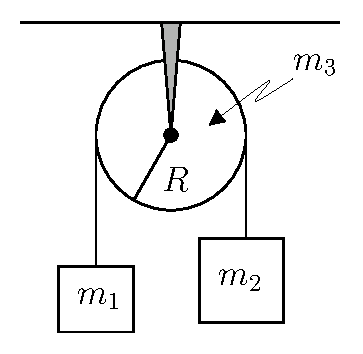
\includegraphics[width=1.7in]{additional_problems/atwood.eps}
    \end{center}
    \caption{Figure for Problem A\ref{prob:pulleywithmass}.}
    \label{fig:atwood}
\end{figure}

\label{prob:pulleywithmass}

\end{aproblem}

\begin{aproblem}{Another Massive Pulley Problem.}

Two objects, each of mass $m$, are connected by
a string of negligible mass that passes over a pulley, as shown.
The surface is frictionless.  The pulley is a uniform disk with
radius $R$ and mass $m_p$, and is free to rotate without friction.
The string does not slip on the pulley.  Find the acceleration of the
hanging object.

\begin{figure}[h]
    \begin{center}
      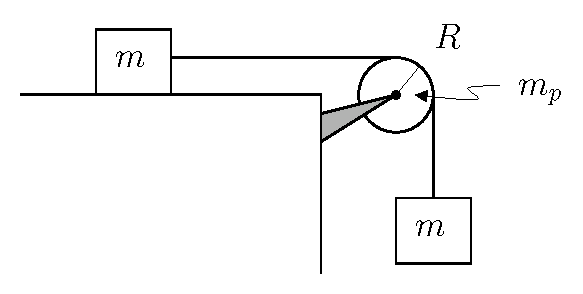
\includegraphics[width=3.0in]{additional_problems/cliff.eps}
    \end{center}
    \caption{Figure for Problem A\ref{prob:anotherpulleywithmass}.}
    \label{fig:cliff}
\end{figure}

\label{prob:anotherpulleywithmass}

\end{aproblem}

\newpage

\begin{aproblem}{Earth's Gravity at the Moon.}
\begin{enumerate}
\item Calculate the magnitude $g$ of the Earth's gravitational field 
at the location of the Moon.  
\item Use your result from part (a) to calculate the gravitational 
force of the Earth on the Moon.  
\item Use your result from part (a) to calculate the gravitational force 
of the  {\it Earth} on a $70\units{kg}$ astronaut standing on the 
surface of the Moon.
\end{enumerate}
\label{problem:gravity_earth_on_moon}
\end{aproblem}

\begin{aproblem}{Gravitational Field via Integration I.}
A rod lies on the $x$-axis with one end at
$x=L_1$ and the other end at $x=L_2$.  The rod is not uniform, and its
mass per unit length varies as $\lambda = Cx$, where $C$ is a
constant.  
\begin{enumerate}
\item Determine the total mass of the rod.  
\item Find the gravitational field at the origin due to the rod.
\end{enumerate}

\begin{figure}[h]
    \begin{center}
      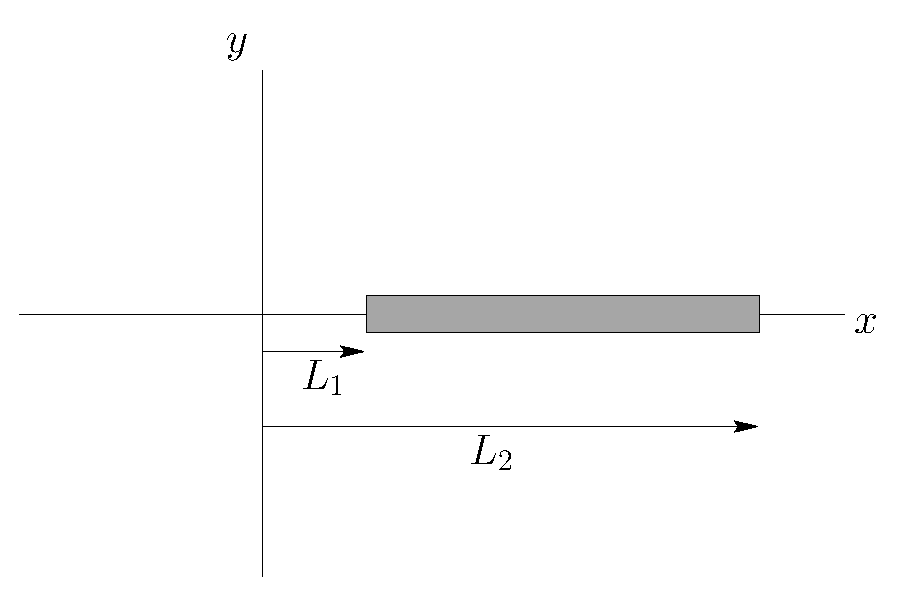
\includegraphics[width=3.0in]{additional_problems/nonuniform_rod.eps}
    \end{center}
    \caption{Figure for Problem A\ref{prob:nonuniform_rod}.}
    \label{fig:nonuniform_rod}
\end{figure}

\label{prob:nonuniform_rod}
\end{aproblem}

\begin{aproblem}{Gravitational Fields.}
Determine the magnitude $g$  of the gravitational field 
\begin{enumerate}
\item on the surface of the Moon (due to the Moon), and 
\item at a point $2000\units{km}$ above the Earth's surface (due to the Earth).
\end{enumerate}

\end{aproblem}

\begin{aproblem}{Gravitational Field via Integration II}
  A uniform rod of mass $M$ and length $L$ lies along the $x$-axis with 
  its center at  the origin.  Determine the gravitational field at the 
  point $x=d$, where $d>L/2$.
\end{aproblem}

\begin{aproblem}{Static Friction}
  Refer to Figure 5.27 in Wolfson (3$^{\rm nd}$ ed.). Let's say that the
  guy there is pulling on the rope, but the trunk is completely motionless
  (and remains that way --- it doesn't budge). Calculate the magnitude of 
  the friction force acting on the trunk in terms of the mass $m$ of the 
  trunk, the tension $T$ in the rope, the angle $\theta$ between the rope 
  and the horizontal, the gravitational acceleration $g$, and the mass 
  $M_J$ of the planet Jupiter.
\label{problem:static_friction}
\end{aproblem}

\begin{aproblem}{Work, Kinetic Energy, and Dissipation}
You throw a $150\units{g}$ baseball straight down from a 
sixth-story window $16\units{m}$ above the ground.  The initial 
downward speed is $7.2\units{m/s}$.  
\begin{enumerate}
\item Calculate the work that gravity does on the ball as it falls to the 
ground.  
\item Assuming that air resistance does $-12\units{J}$ of work on the ball, 
use the work-kinetic energy theorem to calculate the speed of the ball 
when it hits the ground.
\end{enumerate}
\label{problem:W-KE-baseball}
\end{aproblem}

\begin{aproblem}{Recoil on Ice}
  A $42\units{kg}$ child stands at rest on the surface of a frozen pond (i.e., 
  a frictionless surface).  She catches a $1.1\units{kg}$ ball moving 
  horizontally at $9.5\units{m/s}$.  Calculate her speed immediately after 
  catching the ball.
\label{problem:recoil_on_ice}
\end{aproblem}

\begin{aproblem}{Angular Momentum of Point Masses}
  The figure shows 3 objects each with mass $2.0\units{kg}$, and each
  moving with a speed of $4.5\units{m/s}$.  But the objects are traveling
  in different directions, each denoted by an arrow.  Determine the 
  angular momentum about the origin for each of objects A, B and C.

  \begin{figure}[h]
    \begin{center}
    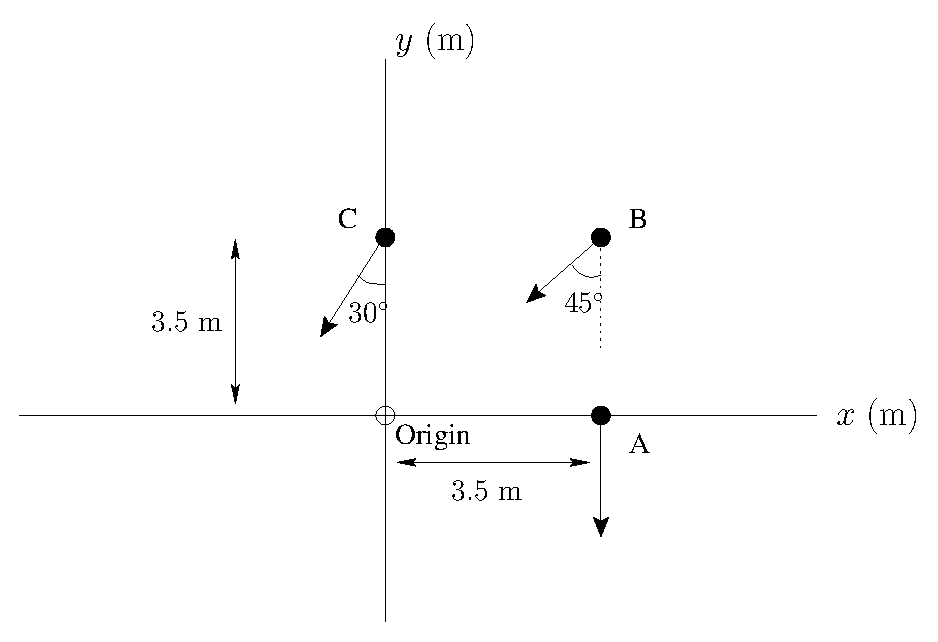
\includegraphics[width=4.0in]{additional_problems/simple_angmom.eps}
    \end{center}
    \caption{Figure for Problem A\ref{problem:simple_angmom}.}
  \end{figure}

\label{problem:simple_angmom}
\end{aproblem}

\newpage

\begin{aproblem}{Molecular Descriptions} 
Answer each part of this question by considering the behavior of 
individual molecules.
\begin{enumerate}
\item Considering the motion of individual molecules in a solid, what
is the difference between a colder solid and a warmer solid?
\item What is the difference between a solid just below its melting
temperature and a liquid just above this melting temperature?  Again,
answer this question  by discussing the behavior of individual molecules
in the solid/liquid.
\item What is the difference between a cooler liquid and a hotter liquid?
\item What is the difference between a liquid just below the boiling
temperature and a gas just above this boiling temperature?
\item What is the difference between a cooler gas and a hotter gas?
\end{enumerate}
\end{aproblem}

\begin{aproblem}{Triple Star System}
Consider a system of three co-linear stars, each with mass $M$, with a 
distance $a$ separating them.  The two outer stars orbit in a 
circle about the the stationary central star.  Determine the square 
of the orbital period, $T^2$.   

\begin{figure}[h]
    \begin{center}
    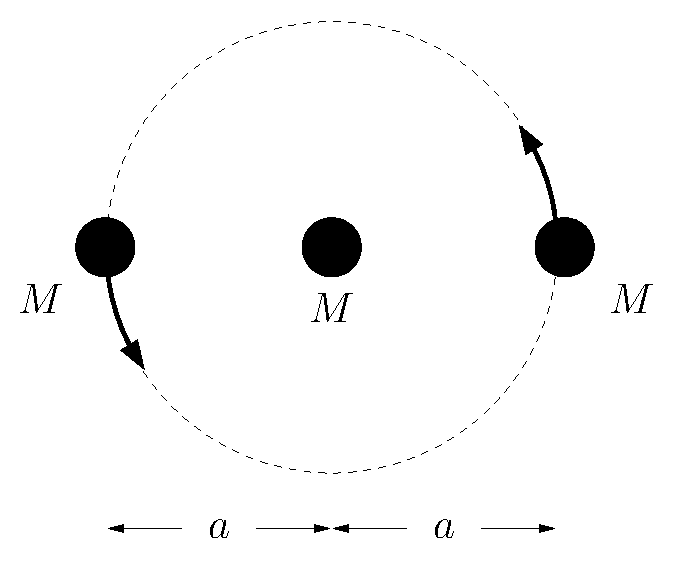
\includegraphics[width=3.0in]{additional_problems/triple_star.eps}
    \end{center}
    \caption{Figure for Problem A\ref{problem:triple_star}.}
  \end{figure}

\label{problem:triple_star}
\end{aproblem}
\newpage

\begin{aproblem}{Tarzan}
A $17\units{m}$ vine hangs vertically from a tree on one 
side of a  $10\units{m}$-wide gorge.  Tarzan wants to 
run toward the vine, grab ahold of it, swing over the gorge, let go of the 
vine, and drop vertically to the ground on 
the other side of the gorge.  How fast must he run to make 
sure that he makes it across the gorge? 

\begin{figure}[h]
    \begin{center}
    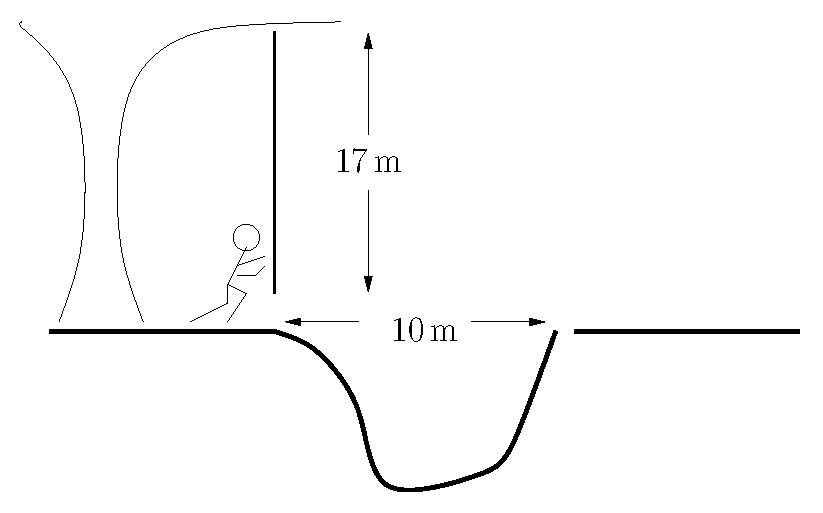
\includegraphics[width=3.0in]{additional_problems/tarzan.eps}
    \end{center}
    \caption{Figure for Problem A\ref{problem:tarzan}.}
  \end{figure}

\label{problem:tarzan}
\end{aproblem}

\begin{aproblem}{Return of Work, Kinetic Energy, and Dissipation}
Repeat part b) of Problem A\ref{problem:W-KE-baseball}, but this time,
instead of using the work-kinetic energy theorem, use 
$W_\text{nc} = \Delta E_\text{mech}$.  Do you get the same answer for 
the speed of the ball?
\label{problem:W-KE-baseball_II}
\end{aproblem}

 \begin{aproblem}{A Bleching Blarg -- Checking Dimensions of Answers}
 A blarg with mass $m$ blechs for a time $T$, after which it flomps
a distance $d$ under the influence of a srof $F_0$ with dimensions
(mass $\times$ distance)/(time)$^2$.  For each of the following
choices, determine if the expression could represent the speed
(dimensions distance/time) of the blarg after all of this.  {\bf Show
your work for each case} (there might be more than one correct
answer).

 (a) $\frac{F_0T}{md}$ \quad 
 (b) $\frac{md}{F_0T}$ \quad 
 (c) $\frac{F_0T}{m}$ \quad
 (d) $\frac{F_0d}{m}$ \quad
 (e) $\frac{m}{F_0d}$ \quad
 (f) $\sqrt{\frac{F_0d}{m}}$ \quad
(g) $\sqrt{\frac{m}{F_0d}}$.
\label{problem:blarg_dimensions} 
\end{aproblem}

\begin{aproblem}{Dimensions for a Florphtl}
A florphtl with length $L$ (in m) and mass $m$ (in kg) has an initial
speed $v$ (in m/s). The florphtl is in a magnetic field $B_0$ (in
units of T where 1 T = 1$\frac{\text{kg}}{\text{C}\cdot\text{s}}$) and
experiences an electrical current $I_0$ (in C/s).  Which of the
following could be an expression for the acceleration (m/s$^2$) of the
florphtl?  (Don't worry about what a ``T'' or ``C'' are -- you'll want
these units to cancel out in the final answer anyway.)

(a) $\frac{mvLB_0}{I_0}$ \quad 
(b) $\frac{mvL}{I_0B_0}$ \quad
(c) $\frac{I_0B_0}{mvL}$ \quad
 (d) $\frac{I_0B_0L}{mv}$ \quad
(e) $\frac{mv}{I_0B_0L^2}$ \quad 
(f) $\frac{I_0LB_0}{m}$.
\label{problem:florphtl_dimensions}
\end{aproblem}

\newpage

\begin{aproblem}{Using ratios}
\begin{enumerate}
\item In a traffic jam on Interstate I-5 near Los Angeles, assume that 
there are 6 cars every 100 feet. How many cars would you expect to
be stuck in 1.0 km of one of these traffic jams?  
\item Let's say that a 9-inch diameter pizza at Francesco's costs
\$12.50. How much should Francesco charge for a 12-inch diameter
pizza, if the cost is determined solely by the total amount of the
ingredients used to make the pizza?
\end{enumerate}
\label{problem:ratios_trafficandpizza}
\end{aproblem}

\begin{aproblem}{Ball pits}
The ``ball pit'' at Dunking Bird Amusement Park measures 11~m by 9~m
with a depth of 60~cm.  Assume that this ball pit contains 8000 balls.
The ball pit at Fred's Amusement Park measures 13~m by 8~m with depth 
40~cm, but uses balls that are half the diameter of those at Dunking
Bird Park.  Approximately how many balls are needed to fill the pit at
Fred's Park?
\label{problem:ratios_ballpit}
\end{aproblem}

\begin{aproblem}{Period of Asteroid Orbit}
The asteroid {\em Betty} orbits the Sun with a semi-major axis of
3.8 AU.  Use Kepler's Third Law (and ratios) to determine the
period (in years) of Betty's orbit.
\label{problem:asteroid}
\end{aproblem}

\begin{aproblem}{Jupiter's Moons}
Jupiter's moon {\em Io} orbits Jupiter with a semi-major axis
421,700 km and an orbital period of 1.8 days.  Another moon --
{\em Ganymede} -- orbits Jupiter with a semi-major axis of
1,070,000 km.  Calculate the orbital period of Ganymede.
\label{problem:Jupiter_Moons}
\end{aproblem}

\begin{aproblem}{Extrasolar planets}
The planet Zortox orbits around the star Xyl'pron with a semi-major
axis of 570 klorvm and an orbital period of 2.7 flurps.  Another
planet -- Rotnox -- also orbits around Xyl'pron with an orbital
period of 7.3 flurps.  Determine the semi-major axis for
Rotnox's orbit.
\label{problem:extrasolar}
\end{aproblem}

\begin{aproblem}{Why you will do badly on tests if you don't show all work}
A 3.5 meter long piece of rope has a mass of 250 g. Your goal is to determine
the mass of a 7.0 meter long piece of the same rope. 
\begin{enumerate}
\item Do this
calculation in your head and then write down the answer on your paper.
\item Do this calculation again, but write down the steps and your reasoning
on the paper.
\item  Scribble out or erase every number and unit for parts
(a) and (b).  Now grade your work from parts (a) and (b) on a 0--10 point
scale for each, basing the grade on how well someone could understand
what you did and why from whatever remains visible on the page after
the numbers and units have been erased or scribbled out.
\end{enumerate}
\label{problem:showyourwork}
\end{aproblem}

\newpage

\begin{aproblem}{Science Fiction and the Laws of Physics}
The following is a science fiction story that is inconsistent with the
known laws of physics.  Read the passage, and then list 4 {\em different}
aspects of the story that are clearly inconsistent with the laws of physics
as covered in PHYS 211 this semester.

\begin{quote}
The Starship Enterprise is on a mission 5 light years from the Earth,
traveling at 7 times the speed of light while being chased by a
hostile Borg ship. ``At our current speed, the Borg won't catch us
for another hours,'' says Captain Picard to Admiral Janeway (who is
back on Earth) on his iPad 563 as he stares at an ice cube floating
lazily in equilibrium with the liquid in his iced tea. ``Well, if they
catch up with you,'' replies Janeway, ``fire a beam of anti-matter
at the Borg ship. The anti-matter will annihilate part of the ship,
and the kinetic energy that is produced by the resulting mass loss
will blow up the rest of the ship.'' ``Understood,'' replies
Picard as he adds another ice cube to his tea, dropping its temperature
down even more.

Just at that moment, Picard is thrown from his chair as a
torpedo from the Borg ship slams into the Enterprise's engines from
behind. ``Our engines have been destroyed~'' says Geordi LaForge as
the ship suddenly comes to a complete halt, motionless in space as
the Borg ship close in.  ``Borg ship,'' radios Picard, ``this is the
Starship Enterprise. We are prepared to talk with you.''
``Prepare to be assimilated,'' replies the Borg ship. ``Resistance
is fut -- ...''.  ``End communication,'' says Picard as the Enterprise
fires, blowing up the Borg ship.
\end{quote}
\label{problem:startrek}
\end{aproblem}


\chapter[Numerical Iteration]{Solving Equations of Motion Using 
Numerical Iteration}
\label{chapter:numerical}

%\section*{Objectives}
%\begin{objectives}
%\item Know what is meant by a numerical iteration method for solving
%  an equation of motion.
%\item Given the initial position and velocity of a particle acted on
%  by a force in one dimension, calculate the position and velocity
%  several time increments later.
%\end{objectives}

\section{Introduction}

The past few decades have witnessed a massive revolution in the way
people live and work, due in great part to {\em significant} enhancements
in computational power.  Computers are everywhere these days in society,
not just on your desktop (or on your lap) but also in your pockets
(MP3 players and cell phones), in your kitchens (ranges, dishwashers
and microwave ovens), and behind the scenes monitoring the money in
your bank accounts, your class schedules and grades, and your music
preferences at on-line music stores.  

The significant enhancement in
computation power has also dramatically changed all fields of science
and engineering.  Despite our brilliant teaching of physics
in this course, there are many problems in physics and engineering that
you simply will not be able to solve analytically.\footnote{By ``analytically''
we mean using the tools from mathematics to determine a written solution
in the form of an equation that can be used to describe the behavior of the
system.}  Some problems simply don't allow a closed-form solution.
But it is even more severe than that.  There are a wide variety of
physical systems whose equations of motion {\bf can't} be solved, 
no matter how brilliant or persistent the 
scientist/mathematician.  In fact, many real systems are ``chaotic,''
with surprisingly complicated behavior arising from seemingly simple
systems.  In cases where an analytical solution is unavailable, the 
only option is to solve the problem {\em numerically}, using a 
computer to simulate the behavior.

Computer simulations have become among the most important techniques
in science and engineering.  Many of you will use numerical techniques
in your career, whether you are simulating the behavior of a new
passenger airline that you are designing, calculating the forces acting
on an artificial joint that you are designing for a patient, or predicting
the effects of a disruption in Middle East oil supply on the global
economy.  Numerical simulations also play a significant role in basic
scientific research, enabling us to explore the behavior of a system that
is too complicated to solve analytically and to difficult to
explore experimentally.  In fact, numerical simulations are so
common now that they are often considered to be a third branch in
scientific analysis, separate from (and complementary to) experimental
and theoretical science.

The basic idea of numerical simulations is actually quite easy.  
In this chapter, we introduce an important technique referred to as 
{\em iteration} where we break the dynamics of the system into 
a series of discrete time steps.  So, for example, instead of 
representing the motion of a ball with a continuous equation, we
instead note the location of the ball, say, every tenth of a second.
Given the location and velocity of the ball at a particular moment
in time, we can predict its location 0.1 s later by using a very 
simple numerical techniques referred to as the
{\em Euler Method}, a technique that conceptually is nothing more
than a simple application of the common ``distance = speed $\times$ time''
approach.  Despite the simplicity of the Euler method, it is a very
powerful method that is used in many numerical applications.  This chapter
introduces the basic ideas (with some homework problems); you will use
the method in lab to simulate the motion of a falling object subject
to air resistance.

\section{Solving Newton's second law analytically}

Newton's second law $\vec{F}_{\rm net} = m\vec{a}$ is a {\em
differential equation}, i.e., an equation that can be written in
terms of derivatives of various quantities.  Ideally, we would like
to ``solve'' this differential equation to 
determine expressions (as a function of time) for the velocity and
position of a particle moving under the influence of the forces.
If the forces exerted on the particle are
all known, then Newton's second law can be rewritten as
\begin{equation}
  a_x = \frac{d^2x}{dt^2} = \frac{F_{{\rm net},x}}{m},
  \label{eq:newtonII}
\end{equation}
where the forces are assumed to be possibly functions of position and
velocity.  Eq.~(\ref{eq:newtonII}) written in that form is known as
the {\em equation of motion} for the system under consideration.
Mathematically one would proceed by integrating Eq.~(\ref{eq:newtonII}) 
to determine the velocity as a function of time
$v_x(t)$ and then integrating once again to obtain the position as a
function of time $x(t)$.  For example we have learned that for a
particle falling from rest from a height $x_0$ under the force of
gravity $F_{\rm net} = mg$, Eq.~(\ref{eq:newtonII}) becomes
\begin{equation}
  \frac{d^2x}{dt^2} = -g,
  \label{eq:eom-freefall}
\end{equation}
and integrating we obtain the following expressions for the velocity
and position:
\begin{equation}
  v_x(t) = -gt \mbox{\hspace{0.25in}and\hspace{0.25in}}x(t) = x_0 - 
  \frac{1}{2}gt^2.
\end{equation}
If you don't understand how we got these expressions, then take the
derivative with respect to time of $x(t)$ to get $v_x(t)$ and then
$v_x(t)$ to get back to Eq.~(\ref{eq:eom-freefall}).

For the example shown above as well as a few other cases, the equation
of motion is relatively straightforward to integrate to get the
analytical functions for velocity and position.  As discussed in the previous
section, though, there are many cases
where the equations of motion are not so easy to integrate and other
means are necessary for determining the position and velocity of the
particle as a function of time.

In the following sections we will develop a set of equations that we
can use to calculate the position and velocity of a particle at
specified time increments $\Delta t$, a technique called {\em
  numerical iteration}.  Although this technique does not give us as a
final result a neat, compact formula for the position and velocity of
the particle into which any value of time can be inserted, it does
allow us to map out the position and velocity of the particle for an
otherwise mathematically intractable problem.

\section{Numerical Stepping Equations}

Let us incorporate the ideas mentioned above into a set of formulas
that we (or better yet, a computer) could use to calculate the
position and velocity of a particle moving under the influence of some
forces.  Call the present time $t$ and the time a little later $t +
\Delta t$.  Let $x(t)$ denote the position of the particle now, then
$x(t + \Delta t)$ denotes the position of the particle a short time
later.  Similarly $v_x(t)$ and $v_x(t + \Delta t)$ represent the present
and slightly later velocities of the particle.  In all of these
expressions, note that $x(t + \Delta t)$ does not mean the quantity
`$x$' times the quantity `$t + \Delta t$' but rather means the value
of the function $x$ evaluated at the time $t + \Delta t$.  This is
standard functional notation used in mathematics.

Recall the definition of velocity as the rate of change of the
position.  Taking $\Delta t$ to be very small in magnitude, we may
approximate this as ``velocity = displacement/time'' and
express the velocity at time $t$ approximately as
\begin{equation}
  v_x(t) \simeq \frac{\Delta x}{\Delta t} = \frac{x(t+\Delta t) - x(t)}
  {\Delta t}.
\end{equation}
As you recall, $\Delta x/\Delta t$ is the definition of the average
velocity, while the instantaneous velocity is actually the derivative
of the position with respect to time.  However, for small enough time
steps, the average velocity is an excellent approximation for the
instantaneous velocity.

Turning the previous expression around, we can write an expression for
the position of the particle at time $t + \Delta t$ in terms of the
position and velocity at time $t$:
\begin{equation}
  x(t+\Delta t) = x(t) + v_x(t)\Delta t.
  \label{eq:x-step}
\end{equation}

Eq.~(\ref{eq:x-step}) says that the position at time $t + \Delta t$ is
the position at time $t$ plus the distance traveled $v_x(t)\Delta t$ by
the particle during the short time interval $\Delta t$.  Notice that
this result is only approximate because the velocity $v_x$ at time $t$
is not necessarily equal to the average velocity during the entire
time interval.  However, if $\Delta t$ is small enough, the
approximation should be quite good.
   
Next we need an expression for incrementing the velocity.  By analogy
with the arguments leading up to Eq.~(\ref{eq:x-step}), we can write
\begin{equation}
  v_x(t+\Delta t) = v_x(t) + a_x(t)\Delta t.
  \label{eq:v-step}
\end{equation}

The three equations (\ref{eq:newtonII}), (\ref{eq:x-step}) and
(\ref{eq:v-step}) can now be incorporated into a looping procedure in
a computer program.  These three equations constitute what is
generally referred to as {\em Euler's method} of numerical
approximation.  Given an initial position and velocity, we calculate
the initial acceleration from Eq.~(\ref{eq:newtonII}).  Then we
calculate the position and velocity a short time later from
Eqs.~(\ref{eq:x-step}) and (\ref{eq:v-step}).  Then we repeat the
process, pretending that the new values for $x$ and $v_x$ are the
initial values.  In this way we can numerically iterate the motion of
the particle from instant to instant as far into the future as we care
to.  A spread-sheet program, such as EXCEL, can perform such
calculations with very little ``programming'' required on your part.

A note about numerical errors is worth mentioning.  Remember that
although Eq.~(\ref{eq:newtonII}) is exact, Eqs.~(\ref{eq:x-step}) and
(\ref{eq:v-step}) that update $x$ and $v_x$ to later times are
approximations that are best when $\Delta t$ is small.  If the
calculations start going haywire, we can help the situation by
choosing smaller steps.  This means of course that the computer will
have to run longer, but that's frequently not a serious problem.

\section{Numerical Solution for a Mass on a Spring}

Let's apply this new method to a system we will be studying more in
depth later in this course.  The system is a mass which moves under
the influence of a force exerted on it by a spring.  The spring is a
device which exerts a force which is proportional to the displacement
of the mass from an equilibrium position.  Taking the equilibrium
position to be $x = 0$, this implies that the acceleration of the mass
is directly proportional to the position $x(t)$.  Suppose in our
particular system the acceleration is given by 
\begin{equation}
a_x(t) = -2.00\, x(t).
\end{equation}
The minus sign in this expression tells us that the force is
always opposite to the displacement.  We'll also assume that time is
in seconds, position is in meters, velocity is in meters per second,
and acceleration is in meters per second squared
   
To proceed, we choose time steps of size $\Delta t = 0.10$ s and start
the clock at $t = 0$.  We could pick any initial position and
velocity; let's choose to release the mass from rest at a position
0.30 m from equilibrium, i.e. $x(0) = 0.30$ m and $v_x(0) = 0$.  Let's
walk through the first few steps and then show some results from a
computer spreadsheet.
   
For our example Eqs.~(\ref{eq:newtonII}), (\ref{eq:x-step}) and
(\ref{eq:v-step}) are written as
\begin{align}
a_x(t) &= -2.00\, x(t) 
\label{eq:ex-a}\\
x(t+0.10) &= x(t) + 0.10\, v_x(t) 
\label{eq:ex-x}\\
v_x(t+0.10) &= v_x(t) + 0.10\, a_x(t).
\label{eq:ex-v}
\end{align}
First calculate the initial acceleration by setting $t = 0$ in
Eq.~(\ref{eq:ex-a}) to find
\begin{equation}
a_x(0) = -2.00\, x(0)  = -2.00 \times 0.30 = -0.60.
\end{equation}
Then update $x(t)$ and $v_x(t)$ by setting $t = 0$ in Eqs.~(\ref{eq:ex-x}) and 
(\ref{eq:ex-v}):
\begin{align}
x(0.10) &= x(0) + 0.10\, v_x(0) = 0.30 + 0.10\times 0 = 0.30 \\
v_x(0.10) &= v_x(0) + 0.10\, a_x(0) = 0 + 0.10\times(-0.60) = -0.06.
\end{align}
Since the mass was initially at rest, a short time later it is still
approximately at the same location.  However, since the spring is
stretched at $t = 0$, a force is acting on the mass immediately, so
that a short time later it has already acquired a non-zero velocity.
   
How would you find $x(0.20)$ and $v_x(0.20)$?  Again use
Eqs.~(\ref{eq:ex-a}) through (\ref{eq:ex-v}), this time with the
`present time' $t = 0.10$.  We find that
\begin{align}
a_x(0.20) &= -2.00\, x(0.10) = -2.00\times 0.30 = -0.60\\
x(0.20) &= x(0.10) + 0.10\, v_x(0.10) \nonumber \\
        &= 0.30 + 0.10 \times (-0.06) \nonumber \\
        &= 0.294 \\
v_x(0.20) &= v_x(0.10) + 0.10\, a_x(0.10) \nonumber  \\
        &= -0.06 + 0.10\times(-0.60) \nonumber \\
        &= = -0.12.
\end{align}
We can continue this process as long as we like.  You will find it
convenient to organize the information for the position, velocity and
acceleration for each time in the form of a table.  Table
\ref{table:numerical1} on the next page lists $t$, $x$, $v_x$ and $a_x$ for
the motion of this mass.  Note that the periodic nature of the motion
is manifested in the entries of the table.  

There is an unsettling aspect of the entries in Table
\ref{table:numerical1}.  We started at $x = 0.30\, \mbox{m}$, but at
$t = 2.30\, \mbox{s}$ the position of the mass is $x = -0.375\,
\mbox{m}$, and further down in the table we find that at $t = 4.5$ s,
$x = 0.468\, \mbox{m}$.  What should we have expected?  If we had a
real mass connected to a spring and set it oscillating we would expect
the amplitude of the oscillations to gradually decrease because of the
presence of dissipative forces (air resistance and the imperfect
elasticity of the spring).  In an ideal case, with no dissipative
effects, we would expect there to be no increase or decrease in the
amplitude; that is, the mass should oscillate between $x = +0.30\,
\mbox{m}$ and $x = -0.30\, \mbox{m}$.  But this is not the case if we
look at the data in Table \ref{table:numerical1}.  The problem is that
we used too large a time increment.  Why does too large a time
increment lead to errors?  If you recall, our stepping equations use
the approximation that the average velocity is very close to the
instantaneous velocity.  If the time step is too large, this
approximation is no longer valid and leads to errors.
   
We can improve our calculation of the motion by choosing a smaller
time increment $\Delta t$.  If we choose $\Delta t = 0.01\, \mbox{s}$
rather than $0.10\, \mbox{s}$, we would be calculating over a much
finer time interval (10 times smaller) and while we will have to do 10
times more computations to evolve the motion out to the same time, the
calculations should be more accurate.  Table \ref{table:numerical2}
lists $t$, $x$, $v_x$ and $a_x$ near a point of maximum displacement for
this smaller time increment.  The maximum displacement is now about
0.314.  This is still larger than the initial displacement but not
nearly as bad as before.  Further reduction of the time increment
would improve the result.

%%% I had to mess around a lot to get floats to appear correctly.  ML

\addtolength{\textheight}{.5in}
\addtolength{\footskip}{-2.in}
\mbox{}
\vspace{-2.in}

\twocolumn

\begin{table}[!t]
\caption{Numerical solution for motion of 
mass on a spring using $\Delta t=0.10\, \mbox{s}$}
\begin{small}
\begin{center}
\begin{tabular}{cccc}
$t$ & $x(t)$ & $v_x(t)$ & $a_x(t)$ \\
\hline
0	&	0.300	&	0	&	-0.600\\
0.100	&	0.300	&	-0.060	&	-0.600\\
0.200	&	0.294	&	-0.120	&	-0.588\\
0.300	&	0.282	&	-0.179	&	-0.564\\
0.400	&	0.264	&	-0.235	&	-0.528\\
0.500	&	0.241	&	-0.288	&	-0.481\\
0.600	&	0.212	&	-0.336	&	-0.424\\
0.700	&	0.178	&	-0.379	&	-0.356\\
0.800	&	0.140	&	-0.414	&	-0.281\\
0.900	&	0.099	&	-0.442	&	-0.198\\
1.000	&	0.055	&	-0.462	&	-0.109\\
1.100	&	0.008	&	-0.473	&	-0.017\\
1.200	&	-0.039	&	-0.475	&	0.078\\
1.300	&	-0.086	&	-0.467	&	0.173\\
1.400	&	-0.133	&	-0.450	&	0.266\\
1.500	&	-0.178	&	-0.423	&	0.356\\
1.600	&	-0.220	&	-0.387	&	0.440\\
1.700	&	-0.259	&	-0.343	&	0.518\\
1.800	&	-0.293	&	-0.292	&	0.587\\
1.900	&	-0.322	&	-0.233	&	0.645\\
2.000	&	-0.346	&	-0.168	&	0.692\\
2.100	&	-0.363	&	-0.099	&	0.725\\
2.200	&	-0.373	&	-0.027	&	0.745\\
2.300	&	-0.375	&	0.048	&	0.750\\
2.400	&	-0.370	&	0.123	&	0.741\\
2.500	&	-0.358	&	0.197	&	0.716\\
2.600	&	-0.338	&	0.268	&	0.677\\
2.700	&	-0.312	&	0.336	&	0.623\\
2.800	&	-0.278	&	0.398	&	0.556\\
2.900	&	-0.238	&	0.454	&	0.476\\
3.000	&	-0.193	&	0.502	&	0.386\\
3.100	&	-0.143	&	0.540	&	0.285\\
3.200	&	-0.089	&	0.569	&	0.177\\
3.300	&	-0.032	&	0.587	&	0.063\\
3.400	&	0.027	&	0.593	&	-0.054\\
3.500	&	0.086	&	0.587	&	-0.173\\
3.600	&	0.145	&	0.570	&	-0.290\\
3.700	&	0.202	&	0.541	&	-0.404\\
3.800	&	0.256	&	0.501	&	-0.512\\
3.900	&	0.306	&	0.450	&	-0.612\\
4.000	&	0.351	&	0.388	&	-0.702\\
4.100	&	0.390	&	0.318	&	-0.780\\
4.200	&	0.422	&	0.240	&	-0.844\\
4.300	&	0.446	&	0.156	&	-0.892\\
4.400	&	0.461	&	0.067	&	-0.923\\
4.500	&	0.468	&	-0.026	&	-0.936\\
4.600	&	0.465	&	-0.119	&	-0.931\\

\hline
\end{tabular}
\end{center}
\end{small}
\label{table:numerical1}
\end{table}
\newpage

%\mbox{}
\begin{table}[!t]
\caption{Data for mass on a spring near a turning point using  
$\Delta t=0.01\, \mbox{s}$}
\begin{small}
\begin{center}
\begin{tabular}{cccc}
$t$ & $x(t)$ & $v_x(t)$ & $a_x(t)$ \\
\hline
4.190	&	0.293	&	0.155	&	-0.586\\
4.200	&	0.295	&	0.149	&	-0.589\\
4.210	&	0.296	&	0.143	&	-0.592\\
4.220	&	0.297	&	0.137	&	-0.595\\
4.230	&	0.299	&	0.131	&	-0.598\\
4.240	&	0.300	&	0.125	&	-0.600\\
4.250	&	0.301	&	0.119	&	-0.603\\
4.260	&	0.303	&	0.113	&	-0.605\\
4.270	&	0.304	&	0.107	&	-0.607\\
4.280	&	0.305	&	0.101	&	-0.610\\
4.290	&	0.306	&	0.095	&	-0.612\\
4.300	&	0.307	&	0.089	&	-0.614\\
4.310	&	0.308	&	0.083	&	-0.615\\
4.320	&	0.308	&	0.077	&	-0.617\\
4.330	&	0.309	&	0.071	&	-0.619\\
4.340	&	0.310	&	0.064	&	-0.620\\
4.350	&	0.311	&	0.058	&	-0.621\\
4.360	&	0.311	&	0.052	&	-0.622\\
4.370	&	0.312	&	0.046	&	-0.623\\
4.380	&	0.312	&	0.040	&	-0.624\\
4.390	&	0.313	&	0.033	&	-0.625\\
4.400	&	0.313	&	0.027	&	-0.626\\
4.410	&	0.313	&	0.021	&	-0.626\\
4.420	&	0.313	&	0.014	&	-0.627\\
4.430	&	0.314	&	0.008	&	-0.627\\
4.440	&	0.314	&	0.002	&	-0.627\\
4.450	&	0.314	&	-0.004	&	-0.627\\
4.460	&	0.314	&	-0.011	&	-0.627\\
4.470	&	0.313	&	-0.017	&	-0.627\\
4.480	&	0.313	&	-0.023	&	-0.627\\
4.490	&	0.313	&	-0.029	&	-0.626\\
4.500	&	0.313	&	-0.036	&	-0.626\\
4.510	&	0.312	&	-0.042	&	-0.625\\
4.520	&	0.312	&	-0.048	&	-0.624\\
4.530	&	0.312	&	-0.054	&	-0.623\\
4.540	&	0.311	&	-0.061	&	-0.622\\
4.550	&	0.310	&	-0.067	&	-0.621\\
4.560	&	0.310	&	-0.073	&	-0.619\\
4.570	&	0.309	&	-0.079	&	-0.618\\
4.580	&	0.308	&	-0.085	&	-0.616\\
4.590	&	0.307	&	-0.092	&	-0.615\\
4.600	&	0.306	&	-0.098	&	-0.613\\
4.610	&	0.305	&	-0.104	&	-0.611\\
4.620	&	0.304	&	-0.110	&	-0.609\\
4.630	&	0.303	&	-0.116	&	-0.607\\
4.640	&	0.302	&	-0.122	&	-0.604\\
4.650	&	0.301	&	-0.128	&	-0.602\\

\hline
\end{tabular}
\end{center}
\end{small}
\label{table:numerical2}
\end{table}

\onecolumn 
\addtolength{\textheight}{-.5in} 
\addtolength{\footskip}{2.in}



%\addtolength{\textheight}{-2.in}
%\addtolength{\footskip}{2.in}

\newpage

\section*{Problems}

\begin{problem}
  For a certain mass-spring system the acceleration is given by $a_x(t) =
  -0.10\, x(t)$.  Suppose the initial position and velocity are $x(0)
  = 10$ m and $v_x(0) = -1.0\, \mbox{m/s}$.  Calculate $x(t)$ and $v_x(t)$
  at $t = 2\, \mbox{s}$ in two different ways:
  \begin{enumerate}
  \item Use two steps of 1 second each.
  \item Use four steps of $\frac{1}{2}$ second each.  Round only your
    final results to three digits (keep all digits for the
    intermediate calculations).
  \item Why aren't the answers to a) and b) the same?
  \end{enumerate}
  \label{problem:ho-undamped-num}
\end{problem}


\begin{problem}
  A drag force on an object is opposite to its velocity and is often
  proportional to its speed.  Let's immerse the mass-spring system of
  problem (\ref{problem:ho-undamped-num}) in a vat of salad oil so
  that the acceleration becomes
  \[a_x(t) = -0.10\, x(t) - v_x(t)\] 

  Repeat problem \ref{chapter:numerical}.\ref{problem:ho-undamped-num}
  for this acceleration.  Compare the results with those you
  originally got in problem
  \ref{chapter:numerical}.\ref{problem:ho-undamped-num}.  Are the
  results what you might expect when a drag force is present?
\end{problem}


%\input{nonconservative}

\chapter{Basic Postulates of Relativity}
\label{chapter:relativityI}

%\section*{Objectives}
%\begin{objectives}
%\item Be able to state the basic, fundamental principles of
%  relativity, and be able to explain how the various aspects of
%  relativity all follow logically from these basic principles.
%
%\item Know how and when to use the proper time relation to relate time
%  intervals in two different reference frames.
%
%\item Be able to relate length and distance measurements in two
%  different reference frames using length contraction.
%
%\item Be able to transform velocities from one reference frame to
%  another.
%\end{objectives}

\section{Introduction}

Certain numbers immediately bring to mind thoughts or ideas.  For
example, ``101'' makes people think of spotted puppies, ``747''
engenders thoughts of large airplanes, ``911'' is the number that you
call for an emergency or one of the worst dates in the history of our
country, and ``42'' is the answer to the ultimate question of Life,
the Universe and Everything.  And if you mention the number ``1905''
to any physicist, he/she will immediately think of the year in which
Albert Einstein published three papers that completely revolutionized
science and fundamentally changed the way in which we view the
universe.  The first paper\footnote{A. Einstein, Annalen der Physik
  {\bf 17}, 132 (1905).} introduced the idea of photons (particles of
light), an idea which formed one of the cornerstones of quantum
mechanics.\footnote{Interestingly, even though any one of these papers
  would be a monumental lifetime achievement for any mere mortal
  physicist, Einstein received the Nobel prize in physics only for his
  work on photons.}  (You will learn about this next semester in PHYS
212.)  The second paper\footnote{A. Einstein, Annalen der Physik {\bf
    17}, 549 (1905).}  was the first to connect molecular diffusion
--- spreading of an impurity in a motionless fluid --- with random
Brownian motion of the individual impurity molecules, which is regarded
as the first demonstration of the existence of atoms.
   
The third paper had a innocuous title: ``On the electrodynamics of
moving bodies.''\footnote{A. Einstein, Annalen der Physik {\bf 17},
  891 (1905).} But there is nothing even remotely innocuous about the
implications of the theory, now known as Einstein's Special Theory of
Relativity (``special relativity'' for short), presented in that
paper.  Einstein's theory completely changed our conceptions of time
and distance\footnote{\dots and, in fact, establishes that they are
  profoundly related, as we shall see.} and of energy and
matter.\footnote{\dots and, in fact, establishes that they are
  profoundly related, as we shall see.}  The theory also led to an
explanation of how stars generate light --- the fundamental source of
energy in the universe without which life on this planet would not be
possible --- and led to the Earth-shattering (almost literally,
unfortunately) development of nuclear weapons.  The theory also holds
the key to the future development of non-fossil fuel energy sources.
Simply put, you cannot understand how the universe works without
studying Einstein's theory of relativity.
   
This chapter and the following three introduce the main ideas and
implications of the Special Theory of Relativity, which applies to the
motion of objects in {\em inertial} (non-accelerating, or ``free
float''\footnote{Taylor and Wheeler, {\it Spacetime Physics}, 2$^{\rm
    nd}$ Edition, (Freeman, 1992), p.\ 26.})  reference frames.  At the
end of the semester, we will also briefly discuss Einstein's General
Theory of Relativity (``general relativity'' for short), which expands
the theory to account for the effects of acceleration and
gravitational fields.

\section{Preliminaries}
A few definitions will be useful for the next few chapters.
   
An {\em event} is something that happens at a particular
location at a particular time.  It is important to be clear about
this, because relativity deals with how different observers measure
distances and times between events.  For instance, let's say that the
penguin on top of your television set explodes at 7:12 a.m.\ on a
Saturday morning.  You then run 5 km to a large tower where you
capture (at 7:45 a.m.) a small platypus that inexplicably is dressed like a
secret agent and who is trying to thwart your plans to take over
the Tri-State Area.  You could identify two events --- (1) the
explosion of the penguin and (2) your capture of the semi-aquatic,
egg-laying mammal of action (i.e., the platypus) --- and say
that these events are separated by 5 km in space and 33 min in time.
Relativity addresses the question of how a different observer measures
the distance and time between the same two events.  (Preview: not
everyone will agree about the distance and time between events.)
   
% And speaking of observers, we need to define a {\em reference
% frame}.  A reference frame can be thought of as a set of common
% observers subject to the same conditions.  Specifically, we will say
% that several observers are in the same reference frame if they agree
% about the distance and time between any two events.
   
So what do we mean, exactly, by ``different observers,'' and what
are the characteristics of these observers that will determine how
their measurements will differ?  We start by explaining what is meant
by the term ``reference frame.'' You can visualize a reference frame
as a set of rulers (distance measuring devices) and clocks (time
measuring devices) that are arrayed throughout space so that the
position and time of any event can be determined directly.  The distinguishing
feature of a reference frame is that the set of ``rulers'' and ``clocks''
are all at rest with respect to one another.  An observer IN THIS
REFERENCE FRAME is at rest with respect to all the rulers and clocks.
Notice that there can be many observers at different positions
in this reference frame, as long as they are all at rest with respect
to each other and to the measuring tools. All observers in the same
reference frame will agree with each other about the distances and
times between any two events, but they will not agree with observers
in other reference frames moving with respect to their frame.

A particularly important kind of reference frame is an {\em
inertial reference frame}.  Observers in an inertial reference
frame experience no significant acceleration, nor can they discern any
gravitational effects.  In an ideal inertial reference frame, the
observer would be floating free (hence the name ``free float'' that is
sometimes used to discuss an inertial reference frame), because any
non-floating motion would necessarily imply either acceleration or
gravitational effects.  To analyze behavior in the vicinity of very
strong gravitational fields, it is necessary to use general
relativity.
   
Technically, an observer is not in a true inertial reference frame if
she is standing on the surface of a planet since there is gravitation.
However, there are plenty of situations where non-inertial effects are
small enough as to be negligible.  In fact, the gravitation from a
typical planet is small enough so that the non-inertial effects are
negligible, and Special Relativity works perfectly well.  So, for
example, we will often treat observers moving on a constant velocity
train as though they are in an inertial reference frame, even though
there is a small gravitational effect.
   
When dealing with velocities, we have to be careful.  A velocity
technically has meaning only if there is a reference.  So, for
example, if you are in a car and you are traveling 65 mph toward the
West, you are really traveling 65 mph {\em relative to the
surface of the Earth}.  In fact, almost any velocity that people
quote in everyday usage is defined relative to the Earth.
   
\begin{boxittext}
{{\bf In preparation for class}, consider the following question: how
fast are you {\em really} going if you are in the car in the previous
paragraph?}
\end{boxittext}
   
Certainly, anyone who is willing to accept a non-geocentric view of
the universe realizes that there is nothing inherently special about
the earth as a reference frame.  But scientists have long wondered if
there is some preferred universal reference frame from which all
velocities should be defined, some standard by which we could define
{\em absolute velocities} for every object in the universe.
   
In relativity, we will use {\em relative velocities}, i.e.,
velocities will always be defined relative to some reference frame.
In fact, one result of relativity is the realization that this is the
best way to define velocity.  There is no need to choose any special
reference frame for the universe; all the results of relativity work
perfectly well with velocities measured relative to any reference
frame that you might choose.
   
The following statement applies to relative velocities: if observer A
measures observer B to be moving at a (relative) velocity of $\vec{v}$
in a particular direction, then B measures A to be moving at a
(relative) velocity of $-\vec{v}$; i.e., same speed but opposite
direction.

\section{Fundamental Principles of Relativity}

Einstein's Special Theory of Relativity is based on a very simple
premise, namely


\begin{boxittext} {{\bf The Principle of Relativity}: the laws of
    physics are the same for observers in different inertial reference
    frames.}
\end{boxittext}

\noindent Let's say, for example, that Michelle sets up a lab in the
basement of Olin Science while Barack sets up an identical lab inside
a truck that is driving on Route 15 with a constant velocity.
Whatever physics equations (including fundamental constants) Michelle
uses to predict and describe the behavior in her lab should work
equally well for Barack in his lab.

Not only is this an intuitively reasonable statement, but
the argument can be made that the whole field of physics would be
useless if this statement weren't true (along with chemistry, biology
and engineering as well).  After all, what is the point of formulating
a set of laws to describe the universe if they only apply to certain
observers moving in a certain way?
   
The question then boils down to this: what {\em are} the fundamental ``laws
of physics'' that are the same for all observers?  At the beginning of
the 20$^{\rm th}$ century, there were two main cornerstones of physics:
Newton's Laws of Classical Mechanics, and Maxwell's Equations
describing electrical and magnetic fields.  You have already been
introduced to Newton's Laws.  We will be discussing
electricity and magnetism in PHYS 212, but here we highlight some of
the ideas relevant to our discussion of relativity.
   
During the 19$^{\rm th}$ century, there was a tremendous surge of
research to describe electric and magnetic phenomena, culminating in
the integration of electromagnetic theory into a set of four
fundamental laws by James Clerk Maxwell in the late 1800s.  Maxwell's
results not only unified electricity and magnetism into a single,
consistent theory, but also showed for the first time that light is an
electromagnetic wave (you'll learn more about this in PHYS 212).  The
theory also showed how to produce a wide variety of different types of
electromagnetic waves, a prescription that had been successfully
tested during the period between Maxwell's theory and Einstein's work
on relativity.  Suffice it to say that Maxwell's equations were
 (and still are) considered by the scientific community to be one of
the cornerstones of physical law.
   
But there was a problem: by the end of the 19$^{\rm th}$ century, some
theorists 
% --- most notably Hendrik Lorentz and George Fitzgerald ---
attempted to generalize Maxwell's equations to apply in
any reference frame and found that this could not be done within the
framework of Newtonian Classical Mechanics.  There arose
a conflict between the two most widely-accepted cornerstones of
physics: Newton's Mechanics and Maxwell's equations.
   
Here is where Einstein came into the picture.  Whereas few people had
previously had any doubts about the validity of Newtonian Mechanics,
Einstein started from the assumption that Maxwell's Equations of
electricity and magnetism were a fundamental law of physics that were
valid in any reference frame, and then set about re-writing Newton's
Laws (generalizing them, actually) to assure that Maxwell's Equations
would be valid in any reference frame.  (Hence the title of Einstein's
third paper in 1905.)
   
The argument is actually fairly simple.  If Maxwell's Equations are
valid for observers in any inertial reference frame, then not only the
form of the equations but also all the constants should be valid in any
reference frame.  Two of the constants in particular --- the
permittivity of free space $\epsilon_0$, and the permeability of free
space $\mu_0$ combine to give a value $1/\mu_0\epsilon_0 = 9.0\times
10^{16}\units{m$^2$/s$^2$}$, which is the square of the speed of
light when it propagates through a vacuum!  Based on the fundamental
Principle of Relativity (above), the conclusion is staggering.  If
Maxwell's equations formulate a fundamental law of physics, then the
Relativity Principle implies the following consequence
\footnote{Einstein stated the second postulate slightly differently:  
``light is always propagated in empty space with a definite velocity
{\em c} which is independent of the state of motion of the emitting
body.''  It can be shown that the invariance of the speed of light, 
with respect to the motion of the {\em source}, and the invariance of the 
speed of light with respect to the motion of the {\em observer}
are simply consequences of each other.}
:

\begin{boxittext}
{
{\bf The invariance of the speed of light}: The speed of light in a vacuum $c$
is measured to be $3.0\times 10^8\units{m/s}$ by any observer in any inertial
reference frame.
}
\end{boxittext}
   
\noindent Although verified experimentally,\footnote{In fact, an
  experiment by Michelson and Morly in 1895 already indicated the
  invariance of the speed of light in vacuum.} this statement runs
counter to our intuition, based on common experience.  Consider the
following sample problems:

\begin{example}{Classical calculation of relative velocities I.}
  Karen is running down the hall of Olin with a loaded blow dart gun.
  She is running with a constant speed of $5\units{m/s}$ when she sees Brian
  and Jeff standing in front of their lab. While still running, she
  fires a blow dart in their direction.  If the speed of the blow dart
  is $15\units{m/s}$ relative to Karen, how fast is the dart moving with
  respect to
  Jeff and Brian's reference frame?  \solution The answer is what you
  would think --- simply add the speeds to find that the blow dart
  travels at a speed of $20\units{m/s}$ relative to Jeff and Brian.
\end{example}

\begin{exampleb}{Classical calculation of relative velocities II.}
  Brian now picks up his blow dart gun and aims it in Karen's
  direction.  Karen quickly retreats, running away from Brian and Jeff
  with a constant speed of $5\units{m/s}$.  Brian fires a dart toward Karen at
  a speed $15\units{m/s}$ measured from his reference frame.  How fast is the
  dart moving with respect to Karen's reference frame?  \solution Again, the
  result is what you would think --- simply subtract the speeds to
  find that the blow dart travels at a speed $10\units{m/s}$ relative to Karen.
\end{exampleb}

\begin{exampleb}{Speeds of light pulses.}  
  Lord Fa is returning to his home world of Gao.  Approaching the
  planet at speed of $2.0\times 10^8\units{m/s}$ (relative to the planet), he
  sends a beacon of light to Commander Nea stationed on Gao.  This
  pulse of light leaves his ship with a speed $3.0\times 10^8\units{m/s}$
  relative to the ship.  How fast is the pulse moving relative to
  Commander Nea?  \solution Classically, you should expect that
  Commander Nea would view the pulse as moving with a speed of
  $5.0\times 10^8\units{m/s}$.  But this is wrong.  Instead, from her
  reference frame, the pulse is moving with a speed of $3.0\times
  10^8\units{m/s}$!  That's just the way it is with light pulses moving in a
  vacuum --- everyone measures the same speed of $3.0\times 10^8\units{m/s}$,
  regardless of their motion.
\end{exampleb}

You should find the results of the above example to be strange ---
there is nothing in our everyday experience that would lead us to
expect such a result.  But numerous experiments have measured the
speed of light in a wide variety of reference frames, and the
results always agree with the statement of the invariance of $c$.

That the speed of light (in empty space) does not depend on the speed
of its source has been demonstrated so convincingly and the value of
the speed measured so accurately that the value is now defined to be
exactly $299,792,458\units{m/s}$. By combining this definition of $c$ with the
definition of the second (in terms of an atomic clock), we no longer
need an independent definition of the meter.

\section{Time dilation}
\label{section:time-dilation}
The most startling consequence of the invariance of the speed of light
is that it forces us to abandon the notion of absolute time.  This
means the time interval between two events depends on the velocity of
the clocks used to measure the interval.  The following {\em thought
  experiment} should help you understand this concept of the
relativity of time intervals.
   
Imagine three identical clocks constructed as follows.  Each clock
contains a light source that emits a pulse of light toward a mirror
some fixed distance away (see Figure \ref{fig:light-clocks}a).  The
mirror reflects the pulse back toward the source.  When the reflected
pulse returns to the source and hits a triggering device, the source
immediately fires a second pulse, which reflects from the mirror and
triggers a third pulse, and so on.  A count registers in a counter for
each return pulse so the number of counts becomes a measure of elapsed
time.
   
We place two of these light clocks, A and B, a fixed distance apart
and at rest in a reference frame attached to the constant velocity
Earth.  We put the third clock, C, on a spaceship traveling at a
constant velocity $\vec{v}$ relative to the Earth (see
Fig.~\ref{fig:light-clocks}b), and perpendicular to the direction of
travel of the light pulse in the clocks.

\begin{figure}[tbp]
\begin{center}
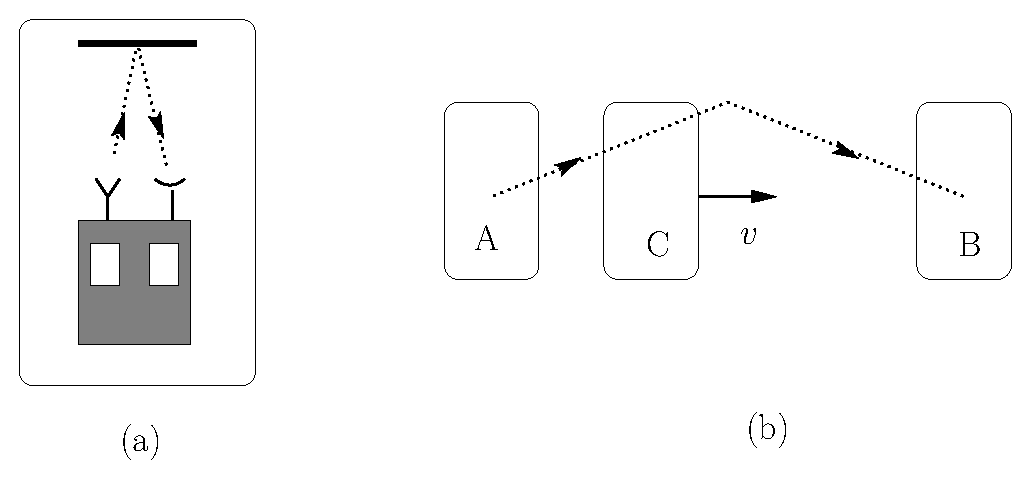
\includegraphics[width=4.5in]{basic_postulates_of_relativity/rel1_clocks.eps}
\end{center}
\caption{(a) A light clock used in the thought experiment described in
  the text. (b) Light clock C passing rest-frame clocks A and B.  The
  dotted line shows the path of C's light pulse as observed in the
  rest frame of A and B.}
\label{fig:light-clocks}
\end{figure}

Suppose clock C emits a light pulse at the exact instant it passes
clock A.  Also suppose that the distance between A and B is such that
clock C passes clock B at the precise instant clock C's reflected
pulse returns to the source.  We therefore have two events: Event \#1
= ``C passes A'' and Event \#2 = ``C passes B.'' We label the time
interval between these two events --- measured by clock C --- as
$\Delta t_C$.  The quantity $\Delta t_C$ is called the {\em proper
  time} interval between the two events; {\bf {\em proper time is
    defined as the time measured on a single clock that is present at
    both events}}.  In the case discussed above, clock C measures the
proper time.  In our particular arrangement, the proper time is
exactly one tick.
   
We now pose the crucial question, the answer to which is the key to
understanding all of special relativity.
\begin{quote}
{\em What is the elapsed time} $\Delta t_{AB}$ {\em as measured by
clocks A and B for clock C to travel from A to B?}
\end{quote}
``Simple,'' you might think.  ``The answer is obviously exactly one
tick, the same as that measured by clock C, right?''  Wrong.  As we
will see, the concepts of absolute time (i.e., everyone and everything
measures the passage of time the say way) is a casualty of the
invariance of the speed of light.
   
For the question posed above to have any meaning, clocks A and B must
be synchronized; i.e., observers in the Earth's reference frame would
say that the two clocks are reading the same time.  (Note: this is not
a trivial matter --- we will discuss synchronization more fully in
Chapter \ref{chapter:relativistic_spacetime}.)  The two-clock time
$\Delta t_{AB}$ is then the difference between the time reading on
clock A at Event \#1 (clock C at clock A) and the time reading on
clock B at Event \#2 (clock C at clock B).
   
In clock C's reference frame, clock A passes C first, and then clock B
passes C.  The time interval between these events is $\Delta t_C$ on
clock C and therefore the light pulse in clock C travels a round-trip
distance equal to $c\Delta t_C$.  But from Fig.~\ref{fig:light-clocks}
this same pulse (the one inside clock C) travels a longer, zig-zag
path when viewed from the frame in which clocks A and B are at rest.
Because of the invariance of the speed of light, {\em this longer
  distance must translate into a longer time interval.}  This means
the round trip time for clock C's pulse is one tick as measured on
clock C, but it is more than one tick when measured on clocks A and B.
In other words, the elapsed time between the event ``C passes A'' and
the event ``C passes B'' is {\em longer} when measured with the two
clocks A and B than when measured with the single clock C.

\begin{figure}[tbp]
  \begin{center}
    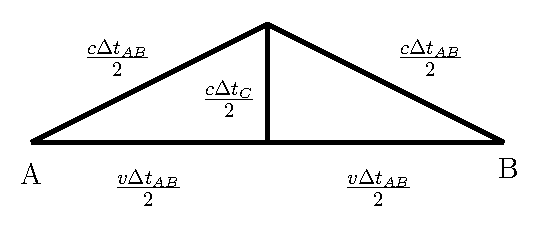
\includegraphics{basic_postulates_of_relativity/rel1_triangle.eps}
  \end{center}
  \caption{Diagram for derivation of the proper time relation.  In 
    this figure $\Delta t_{AB}$ is the elapsed time determined from 
    the clocks A and B, and $\Delta t_C$ is the elapsed time on clock C.}
  \label{fig:rel_triangle}
\end{figure}

How much longer is the time interval $\Delta t_{AB}$ measured on the A
and B clocks than the proper time interval $\Delta t_C$ measured on
clock C?  We can find out by looking at the path taken by the pulse of
light in clock C viewed from C's reference frame and from A and B's
reference frame (see Fig.~\ref{fig:rel_triangle}).  As we've already
seen, in clock C's frame the pulse travels straight up and down along
the vertical line in the figure and the total round-trip distance is
$c\Delta t_C$.  The same pulse, traveling for time $\Delta t_{AB}$
relative to A and B travels the total zigzag distance $c\Delta
t_{AB}$.  Clock C itself travels a distance $v\Delta t_{AB}$ relative
to clocks A and B while the pulse makes one round-trip in C.
Therefore, using the Pythagorean theorem on either small triangle in
Fig.~\ref{fig:rel_triangle}, we find
\begin{equation}
\left(\frac{c\Delta t_{AB}}{2}\right)^2 = 
\left(\frac{c\Delta t_{C}}{2}\right)^2 + 
\left(\frac{v\Delta t_{AB}}{2}\right)^2,
\end{equation}
from which we solve for the proper time $\Delta t_C$ to obtain
\begin{equation}
\Delta t_C = \Delta t_{AB}\sqrt{1 - v^2/c^2}.
\end{equation}
This relation can be written in the general form:

\begin{boxiteq}
{
\begin{equation}
\Delta t_{\rm proper} = \Delta t_{\rm two-clock}\sqrt{1 - v^2/c^2}.
\label{eq:ptr}
\end{equation}
}
\end{boxiteq}

\noindent This very important relation is sometimes called the
``proper time relation'' or the principle of ``time dilation.''
Qualitatively, it expresses the fact that {\bf {\em different
observers measure the passage of time differently depending on their 
relative motion.}}
   
Hidden inside Eq.~(\ref{eq:ptr}) is another result from special
relativity; namely, no object can travel at a speed greater than $c$
relative to any other object or reference frame.  A superluminal speed
($|v| > c$) would result in an imaginary proper time, something that
has no physical meaning.  You will learn later that this speed limit
is imposed by energy considerations as well (it would take an infinite
amount of energy to accelerate an object with mass\footnote{Of course,
a photon of light can be considered an ``object'' that travels at 
a speed $c$, but this is a massless object.  We'll say more about this 
in Chapter \ref{chapter:relativity_pande}.} to a speed $v = c$
relative to an observer, and {\em more} than an infinite amount of
energy to achieve a speed $v > c$).  Therefore, because $|v| \leq c$,
the proper time interval $\Delta t_{\rm proper}$ between two events
is always {\em smaller} than the time $\Delta t_{\rm two-clock}$
measured in a frame that requires two synchronized clocks for
measurement.

   
\begin{example}{Time dilation.}
A father and his daughter are traveling on a train that moves with a 
constant speed of $1.8\times 10^8\units{m/s}$ ($= 0.6c$)
relative to the ground.  They pass a parked VW Beetle at which point
the two of them simultaneously yell, ``Red Punch Buggy!'' and punch each
other on the shoulder.  Three seconds later, the daughter yells,
``Jinx!''  What is the time between these two events according to a
person inside the VW who is waiting for the train to pass?
\solution
The key question ---  who measures the proper time (i.e., the
smaller time interval)?  To answer this, write this down in terms of
events.  Event A $=$ father/daughter punch each other; Event B $=$
daughter jinxes her dad.  In this example, the father/daughter are at
both events (not the person in the car), so they measure the smaller
(proper) time interval, which has already been stated to be $3\units{s}$.  
So, we are given $\Delta t_{\rm proper}$ and we are solving for 
$\Delta t_{\rm two-clock}$, 
which is the time interval measured by the person in the car.
\begin{align}
\Delta t_{\rm proper} &= \Delta t_{\rm two-clock}\sqrt{1-v^2/c^2} \nonumber \\
\Rightarrow \Delta t_{\rm train} &= 
                \Delta t_{\rm VW}\sqrt{1-v^2/c^2}\nonumber \\
\Rightarrow \Delta t_{\rm VW} &= 
                \frac{\Delta t_{\rm train}}{\sqrt{1-v^2/c^2}}\nonumber \\
                   &= \frac{3\units{s}}{\sqrt{1-(0.6c/c)^2}}\nonumber \\
                   &= \frac{3\units{s}}{\sqrt{1-0.6^2}}\nonumber \\
                   &= 3.75\units{s}.
\end{align}
\end{example}

In this example, the father and daughter on the train measured the
proper time because they were at both events, so the time interval is
smaller from their reference frame.  Be careful, though: sometimes the
observer standing on the Earth measures the smaller time interval --- it
all depends on what the events are and who happens to be present at
both of them.
   
Note also that we expressed $v$ as a fraction of the speed of light --- it
makes things a lot simpler to write $v$ in this manner.  We'll say more
about this later

\section{Length contraction}

One thing that will come up repeatedly in this unit is the fact that
relativity breaks down the distinction between distance and time.  In
fact, in relativity, distance and time are really just flip sides of
the same coin.  And as we will see now, you can't change our
conception of time without making a similarly dramatic change in the
way we view distances and length.
   
Consider the following thought experiment: a train is moving on a
track, with Observers A and B at the front and back end of the train.
A and B have measured the length of the train with a long tape measure
that they carry with them on the moving train, and find the length to
be $L_{\rm train}$.  The train goes past Observer C who is standing
next to the track with a stopwatch (see Fig.~\ref{fig:contraction}).
Relative to C in the ``ground reference frame,'' the train is moving
with a speed $v$.  From the train's reference frame, of course, it is
C and the ground that are moving at a speed $v$ in the opposite
direction.
    
   
\begin{figure}[tbp]
\begin{center}
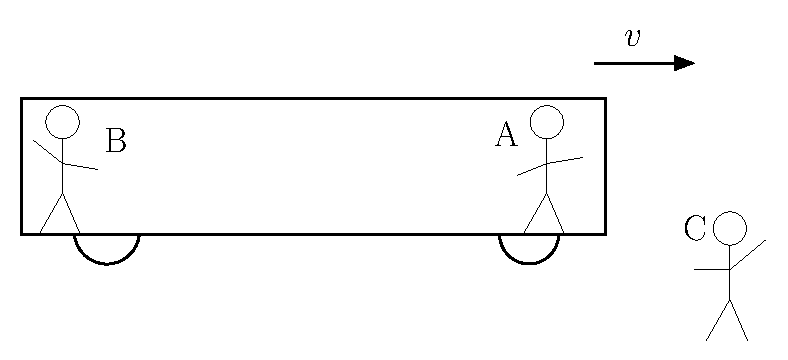
\includegraphics[width=3.5in]{basic_postulates_of_relativity/rel1_train.eps}
\end{center}
\caption{Sketch of train for length contraction thought-experiment.}
\label{fig:contraction}
\end{figure}   
   
Let's say that Observer C wants to measure the length of the train.
He can use his stopwatch to do this: since distance = (speed) $\times$
(time), the length of the train is simply the speed $v$ times the time
interval between when the front of the train passes and when the back
of the train passes.  Let's consider two events: Event A $=$ front of
train passes C; Event B $=$ back of train passes C.  According to
people on the train, the time between the two events $\Delta t_{\rm
  train} = L_{\rm train}/v$, where $L_{\rm train}$ is the
previously-measured length of the train --- this is how far Observer C
moves between the events according to train observers.  But, as we saw
in the previous section, C measures the proper time (since this
observer is at both events), which is a smaller time interval:
\begin{equation}
\Delta t_C = \Delta t_{\rm proper} = \Delta t_{\rm train}\sqrt{1 - v^2/c^2}.
\end{equation}
Based on this result, Observer C now says that the length of the train is 
\begin{align}
 \text{Length} = (\text{speed})\times (\text{time}) &= v\Delta t_C \nonumber \\
                &=  v \Delta t_{\rm train}\sqrt{1-v^2/c^2}  \nonumber \\
                &= L_{\rm train}\sqrt{1-v^2/c^2}.
\end{align}
{\bf {\em The length of the train as measured by an observer by the
side of the track is less than the length of the same train as
measured by people moving with the train.}}

We can write this relation (referred to as the {\bf {\em Lorentz
contraction}} or simply {\bf {\em length contraction}} equation) in
more general terms:

\begin{boxiteq}
{
\begin{equation}    
L_{\rm other} = L_{\rm rest}\sqrt{1-v^2/c^2},
\label{eq:lengthcontract}	
\end{equation}
}
\end{boxiteq}

\noindent where $L_{\rm rest}$ is the length of an object as measured by
observers in a reference frame where that object is at rest, and
$L_{\rm other}$ is the length as measured by observers in a different
reference frame.  Note that an object is always largest when viewed
from its own reference frame, and shrinks when it is viewed as moving.
   
Some comments are in order:  
\begin{itemize}
\item You can't have time dilation without length contraction --- the 
two necessarily go hand-in-hand.  This is a recurring theme of relativity ---
Einstein's theory can't be taken ``a la carte''; rather, it is all or nothing.
Einstein realized that if any single prediction of relativity were
ever refuted, then the entire theory would have to be discarded.  
\item The arguments in this section apply to length components along
the direction of the relative motion.  Components of a length in 
directions perpendicular to the relative motion are not contracted. 
\item Length contraction is not an illusion or merely a matter of
perception.  In the example, the train doesn't just appear to be
smaller from C's reference frame; rather, it  {\em really is
smaller} in that reference frame.  Some of the homework problems and
drill questions will investigate some of the curious properties of
length contraction.
\end{itemize}

\section{Experimental evidence}
   
Most people are skeptical when they first read about the predictions
of special relativity.  This is to be expected, since we do not
experience time dilation or length contraction effects on a daily
basis.  For these effects to be significant, you need relative
velocities that are significant fractions of the speed of light.
Looking at both Eqs.~(\ref{eq:ptr}) and (\ref{eq:lengthcontract}), the
key piece is the stretch factor $\sqrt{1-v^2/c^2}$, which is almost
identically equal to 1.00 for even the fastest velocities that people
ever experience.  This is an important aspect of relativity;
namely, that it obeys classical correspondence, i.e., the results of
relativity agree with Newton's classical results for smaller
velocities.
   
Despite the fact that relativistic effects are almost negligible in
the ``everyday'' phenomena of our personal experience, there is 
copious experimental evidence
that shows that Einstein's predictions are correct.  In every case
where an experiment has tested the theory of relativity, the
experimental results have always agreed precisely with the predictions
of relativity.  Some examples:

\begin{itemize}
\item {\bf Time dilation}.  Time dilation is the most tested aspect of
relativity.  The most direct test was performed by taking two
identical atomic clocks, flying one around the world on a plane and
leaving the other on the ground, then comparing their readings after
the trip.  As predicted by Einstein, the clocks had ticked off
different times, and by precisely the predicted amount.\footnote{Note
that General Relativity plays a role here because the height of a
clock also affects its rate, but the experiments took account of these
general relativistic effects.} Particle decay has also been used to
test time dilation: a type of particle that typically lives for a
certain period of time has been shown to live significantly longer if
accelerated to high speeds (relative to the ground); again, the
difference in times agrees perfectly with relativity.  And the Global
Positioning System (GPS) --- which involves a series of satellites
with precise clocks --- uses relativity extensively to keep the
orbiting clocks synchronized with those in the GPS units on the Earth.
Without relativistic corrections, GPS wouldn't work!
   
\item {\bf The speed of light as a speed limit.}  This result is verified
daily in particle accelerators.  It is fairly straightforward for
scientists to accelerate subatomic particles to speeds close to the
speed of light.  But no matter how much energy is added, the speeds
never make it to or above $c$.  Electrons, in particular, have been
accelerated to speeds $u> 0.99999999999c$, but never up to or above $c$.
   
\item {\bf Length contraction.}  No experimentalist has managed to
accelerate a train to relative speeds large enough to measure length
contraction effects.  (Trust us: you wouldn't want to be anywhere near
a train going this fast.)  But there is experimental evidence for
length contraction: (a) cosmic rays produced at the top of the Earth's
atmosphere somehow manage to make it to the surface of the Earth
before decaying, despite the fact that they are very unstable.  Some
of these particles have lifetimes so short that even traveling at
speeds close to $c$, they would be expected to decay long before they
reach the ground.  This can be explained using length contraction: the
distance from the top of the atmosphere to the Earth's surface is
significantly contracted from their reference frame, so there is no
problem making it to the Earth's surface before
decaying.\footnote{This result can also be explained using time
dilation, of course, because time dilation and length contraction are
really different aspects of the same phenomenon.} (b) Another piece of
experimental evidence comes from electromagnetic theory --- it turns out
that you can explain why an electrical current produces magnetic
effects by applying relativistic length contraction to the stream of
electrons.  The argument is too long to present here (especially since
we haven't covered electricity and magnetism yet), but suffice it to
say that the results agree perfectly with an analysis based on length
contraction.
\end{itemize}
   
There are other experimental tests of other aspects of relativity,
some of which will be discussed later in this unit (when those aspects
are presented).  But, in general, it is worth remembering that
relativity is not a series of different theories, but rather is a
single, coherent, internally consistent theory.  All of the
predictions are inherently related to each other.  So you can't say,
``Well, I'm fine with time dilation but I don't buy length
contraction.''  You simply can't have time dilation without length
contraction --- they are the same thing. So even if there hadn't been
any independent experimental evidence of length contraction (which
there is) there would be very little doubt of its veracity since time
dilation has been verified extensively.

\section{Units and dimensionless velocities}

When working with relativity, it is convenient to express lengths in
terms of distance traveled by light in one unit of time.  A ``light
year'' for instance is the distance that light travels in one year.
An analogy would be to say that the distance between here and New York
City is ``three car hours'' (i.e., it takes 3 hours to get to New York
in a car driving at highway speeds).  In fact, you will often hear
people using time directly to express a distance: ``Oh, it's 3 hours
to New York City from here.''  We will abbreviate these units as lt-s,
lt-min, lt-yr, \dots for light-second, light-minute and light-year,
respectively. Using these units for distance, we can express speeds in
terms of lt-s/s, lt-min/min, lt-yr/yr, etc.  Since the speed of light
$c = 1 \units{lt-s/s} = 1 \units{lt-min/min} = 1 \units{lt-yr/yr} =
\dots$, the speed of a particle in these units is simply the speed
expressed as a fraction of the speed of light.
   
\begin{example}{Units Conversion from lt-s/s to m/s}
  A proton is traveling at a speed of $0.25\units{lt-s/s}$.  Find its speed in
  units of m/s.  \solution Use the fact that $1\units{lt-s/s}$ is equal to
  about $3.00\times 10^8\units{m/s}$.  Then convert units in the
  usual way:
\[ 0.25\units{lt-s/s} \times 
        \frac{3.0\times 10^8\units{m/s}}{1\units{lt-s/s}}
       = 0.75\times 10^8\units{m/s}.  \]
In this example, a particle has a speed $u = 0.25\units{lt-s/s}$.  This same
speed could be expressed as $u = 0.25c$.  In fact, we will typically
express velocities as a fraction of the speed of light $c$.
\end{example}

\newpage

\section*{Problems}
\markright{PROBLEMS}

\begin{problem}
Give a one sentence definition of a meter, using the concept of
a second and the defined value for $c$.  
\end{problem}

\begin{problem}
A proton is traveling at a speed of $4.0 \times 10^7\units{m/s}$.  
How many lt-s/s is this?
\label{prob:rel_units}
\end{problem}

\begin{problem}
A $\pi^-$ meson is traveling at a speed of $0.060\units{lt-s/s}$.  
Convert this speed to m/s. 
\label{prob:rel_units2}
\end{problem}

\begin{problem}
A spaceship moving at constant speed $0.80\units{lt-s/s}$
travels between two planets A and B in $1000\units{s}$, as measured by
synchronized clocks on the planets.  Calculate the elapsed time
according to a clock carried on board the spaceship.  
\end{problem}

\begin{problem}
How fast does a particle have to travel relative to clocks A and
B, which are at rest relative to each other, in order that its elapsed
time as read on a clock moving with the particle is one-tenth the
elapsed time measured on clocks A and B?  Express your answer both in
lt-s/s and in m/s.
\label{prob:time_dilation1}
\end{problem}
  
\begin{problem}
  A meteorite is observed to travel a distance $1.00 \times
  10^5\units{lt-s}$ relative to the Earth in a time of $6.00 \times
  10^5\units{s}$ as measured by Earth observers.  Calculate the
  elapsed time for this trip as measured by a clock carried along on
  the meteorite.
\label{prob:meteorite}
\end{problem}

\begin{problem}
A crew of astronauts travels at a speed of $0.60c$ from Earth to
the nearest star, Proxima Centauri, a distance of $4.0\units{lt-yr}$ 
(as determined by observers on Earth).
   \begin{enumerate}
   \item Calculate how long the trip takes according to observers at
   rest relative to the Earth. 
   \item Calculate the time for the trip as measured by a clock on the
   spaceship. 
   \item Based on your answer to b), calculate the distance from
   Earth to Proxima Centauri as determined by the astronauts using the
   relation ``distance'' $=$ ``speed'' $\times$ ``time'', where 
   distance, speed and
   time are all measured from the astronauts' reference frame.
   \item Calculate the Earth-Proxima Centauri distance from the
   astronauts' reference frame, but this time use length contraction.
   You should end up with the same result as for c).
   \item Think about the results from parts c) and d).  This should
   convince you that length contraction and time dilation are really
   the same thing (i.e., you can't have one without the other).  
   \end{enumerate}
\label{prob:alpha_centauri}
\end{problem}

\begin{problem}
Another spaceship crew wants to make the trip from Earth to
Proxima Centauri in only 2.0 years as measured by clocks on board their
spaceship.  (Recall from the previous problem statement that the 
distance between Earth and Proxima Centauri is $4.0\units{lt-yr}$ 
as determined by observers on Earth.) 
    \begin{enumerate}
    \item How long does the trip take according to Earth-frame observers?
    \item How fast must the astronauts travel relative to Earth? 
    \end{enumerate}
Hint: First, do both parts a) and b) together.  Also, you will need
to express the speed in terms of the unknown travel time according to
Earth-frame observers.  
\label{prob:alpha_centauri2}
\end{problem}

\begin{problem}
You are in a metallic red VW bug stopped at a traffic light.
You see the traffic light turn green, and $2.5\units{$\mu$s}$ later you hear
the car behind you honk its horn.  What is the time between you 
seeing the light change to green and your hearing of the horn honk 
as measured by an 
alien passing by in a ship at a speed $0.9c$?
\end{problem}

\begin{problem}
There is a supergiant star named Betelgeuse\footnote{Betelgeuse
is a supergiant star located in the constellation Orion.  It is very
cool because it could go supernova anytime in the next million years,
and that will be quite a show for us when it does.} which (in the
Earth's reference frame) is $80\units{lt-yr}$ away.  
    \begin{enumerate}
    \item A crew of astronauts is traveling toward Betelgeuse,
    traveling at a speed $0.8c$ relative to the Earth-Betelgeuse
    reference frame.  What is the separation between Earth and
    Betelgeuse in the astronauts' reference frame?
    \item Another crew traveling toward Betelgeuse measures the
    Earth-Betelgeuse distance to be $23\units{lt-yr}$.  How fast is this 
    second crew traveling relative to the Earth?
    \end{enumerate}
\label{prob:betelgeuse}
\end{problem}

\begin{problem}
Betty is standing by the side of a train track when a really
long train approaches traveling at a ridiculously fast speed of $0.9c$.
Thinking quickly, she pulls out her stopwatch, clicks it on when the
front of the train passes and clicks it off when the back of the train
passes.  After standing back up and smoothing down her hair, she notes
that her stopwatch reads $0.0025\units{s}$.  (She has really good reflexes.)
Betty now makes some calculations.
    \begin{enumerate}
    \item According to Betty, how long is the moving train?  (Assume
     that she was warned in advance that the train was going at a
     speed $0.9c$.)
     \item Later that day (not much later), the train reaches its
     destination and stops.  What is the length of the train according
     to people standing next to the (now motionless) train?
     \end{enumerate}
\end{problem}

\begin{problem}
During migration, two fast Arctic terns fly one behind the other
over London at speed $0.8 c$.
%  As they pass the
%border, a guard at the border station notes that
A tourist  sees the birds pass by while looking at the Big Ben clock tower.
She notes that
a time of $12.0\units{ms}$ elapsed on the clock between the first 
bird's passing and the second bird's passing.
    \begin{enumerate}
    \item How much time elapsed between these two events, according to
    the birds?
    \item How far apart are the birds according to the tourists watching the
birds fly by?  
    \end{enumerate}
\label{prob:terns}
\end{problem}

\begin{problem}{\bf Playing Catch on a Train I}\\
{\bf Note:} This is a non-relativistic physics problem.\\
You are riding in a box car of a train that is traveling along the tracks
at $30\units{m/s}$.  You are bored, so you start to play catch with
your friend who is standing on the opposite side of the box car, $5\units{m}$
away from you.  You throw the ball at a speed of $10\units{m/s}$
straight to your friend, who catches the ball; the given speed and direction
are determined in {\em your\/} reference frame.  You may ignore any vertical
motion of the ball.
 \begin{figure}[h]
    \begin{center}
    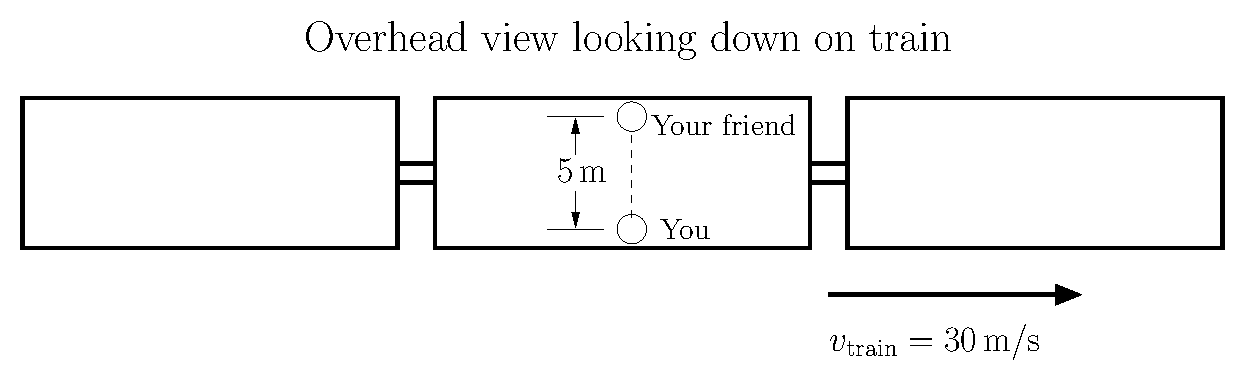
\includegraphics[width=5.5in]{basic_postulates_of_relativity/catch_on_trainI.eps}
    \end{center}
    \caption{Figure for Problem \ref{prob:catch_on_trainI}.  This is
    a top view looking down upon the train.}
    \label{fig:catch_on_trainI}
  \end{figure}
\begin{enumerate}
\item How long does it take for the ball to reach your friend according
to you?
\item How long does it take for the ball to reach your friend according
to an observer standing at rest on the ground?  (This is a dumb question in
classical physics --- if the answer isn't obvious, you're thinking too
hard!)
\item How far does the ball travel according to the observer
standing on the ground?
\item What is the speed of the ball according to the observer
standing on the ground?
\end{enumerate}

\label{prob:catch_on_trainI}
\end{problem}

\begin{problem}{\bf Playing Catch on a Train II}\\
{\bf Note:} This is a non-relativistic physics problem.\\ You are riding in a
box car of a train that is traveling along the tracks at an undetermined
speed.  Once again, you are bored, so you start to play catch with your
friend who is standing on the opposite side of the box car $5\units{m}$
away from you.  (See figure in previous problem.)  You throw the ball
in a horizontal plane at a speed of $10\units{m/s}$ straight to your
friend, who catches the ball.  According to an observer on the ground,
the ball travels a distance of $13.93\units{m}$ between the time you
throw it and the time your friend catches it.  Calculate the speed of
the train along the tracks.
\label{prob:catch_on_trainII}
\end{problem}

\begin{problem}{\bf Photons on a Train}\\
{\bf Note:} This is a relativistic physics problem.\\ Alice is riding
in a box car of a train that is traveling along the tracks at a speed
$v=0.6\units{lt-ns/ns}$.  She just happens to have a light-clock with her
(just like the one illustrated in Fig.~\ref{fig:light-clocks} in Chapter
\ref{chapter:relativityI}).  Alice aligns the clock so that the light
is aimed horizontally directly across the train car, perpendicular to
the motion of the train.  Alice sends a light pulse across the train,
and notices that the light returns to the detector $2\units{ns}$ later.
Alice's friend Bob is standing at rest on the ground as Alice and her
light-clock speed by.  Bob measures the round-trip time for the pulse
of light in Alice's light clock to be $\Delta t_{\rm Bob}$.
\begin{enumerate}
\item What is the speed of the light pulse according to Alice?
\item Determine the distance between the emitter/detector and the mirror
in the light-clock as determined by Alice.
\item  What is the speed of the light pulse according to Bob?  (This is
a dumb question in relativistic physics --- if the answer isn't obvious,
you're thinking too hard!)
\item Determine length of the path traversed by the light pulse according
to Bob {\bf in terms of the unknown time $\Delta t_{\rm Bob}$}.
\item Use the Pythagorean theorem  to find the distance
traveled by the light pulse according to Bob. From this determine
a numerical value for $\Delta t_\text{Bob}$.
% Use your results to determine $\Delta t_{\rm Bob}$.  Do {\bf not}
% use Eq.~(\ref{eq:ptr}) to calculate this result; rather, use the 
% hypotenuse of the right triangle to find the distance the light pulse
% travels according to Bob.

\item Now use Eq.~(\ref{eq:ptr}) to calculate $\Delta t_{\rm Bob}$.
This answer should agree with the answer you determined in the previous
part.
\end{enumerate}
\end{problem}
\newpage


\chapter{Relativistic Spacetime}
\label{chapter:relativistic_spacetime}

%\section*{Objectives}
%\begin{objectives}
%\item Be able to calculate a spacetime interval between two events,
%  and classify the interval as space-like, time-like or light-like.
%  Use these classifications to determine whether or not the two events
%  could be causally linked.
%\item Be able to use the invariance of the interval to relate distance
%  and time intervals in one reference frame to those in a different
%  frame.
%\item Be able to draw and/or interpret a spacetime diagram, and use
%  this diagram to determine temporal and spatial ordering of events,
%  including whether or not events are simultaneous or at the same
%  location.
%\end{objectives}

\section{Introduction}


The previous chapter introduced the basic ideas of relativity along
with some of the most dramatic implications of the theory.  But the
predictions of time dilation and length contraction are merely special
cases of a much broader theory.  In this chapter, we discuss the idea
of spacetime, which blends time and space together.  We introduce the
spacetime interval, a quantity that is one of the fundamental
invariants in relativity, and we use this interval to relate distance
and time measurements made in different reference frames that 
are moving with respect to each other.  We also introduce
spacetime diagrams, which provide a graphical way of illustrating
relativistic phenomena, particularly the relativity of simultaneity.
    
%We also develop the relativistic velocity transformation formulas,
%which allow us to compute a particle's velocity in one inertial frame
%if we know the particle's velocity in another inertial frame.

\section{Spacetime intervals}

\label{sec:spacetime_intervals}

As we saw in Chapter \ref{chapter:relativityI}, observers in different reference frames
disagree about time and distance measurements.  But there are a few
quantities referred to as invariants upon which all observers agree
regardless of their reference frames.  One of these invariants was
discussed in the previous chapter; namely, the invariance of the speed
of light in a vacuum.  It turns out that distance and time can be
folded together to make another invariant, referred to as the
invariant spacetime interval $I$, defined by

\begin{equation}
I^2 \equiv \left(c\Delta t\right)^2 - \left(\Delta x\right)^2.
\label{eq:intervaldef}
\end{equation}
Note that $I^2$ can be positive, zero, or negative.  If $I^2$ is
positive, then the interval is called {\em time-like\/}  since the first term
--- with $\Delta t$ in it --- dominates.  Similarly, negative values
of $I^2$ correspond to {\em space-like\/} intervals, and if $I^2 = 0$, the
interval is called {\em light-like\/}.  Qualitatively, an event is light-like
if a pulse of light could travel directly between the two events.
This can be seen from Eq.~(\ref{eq:intervaldef}): if $I^2 = 0$, then
\begin{align}
0 &= \left(c\Delta t\right)^2 - \left(\Delta x\right)^2  \nonumber \\
\Rightarrow \Delta x &= \pm c \Delta t,
\end{align}
as would be expected for a pulse of light traveling a distance $\Delta
x$ in a time $\Delta t$.

Two events could be {\em causally-linked} (i.e., event A actually
causes or contributes to event B) if the spacetime interval between
them is either light-like or time-like.  In fact, for time-like
spacetime intervals, the interval is the proper time (multiplied by $c$).  
If two events are separated by a space-like interval, then no 
information can travel between the two events since it would require 
superluminal ($|v| > c$) information transmission, and nothing 
(especially information) can travel faster than light relative to 
any observer.  So events {\em can't} be causally linked if the square 
of the spacetime interval between them is negative.


\begin{example}{Causality and intervals}  
  In the year 2055, a father and his daughter are watching the 5$^{\rm
    th}$ game of the National League Divisional Series from a Moon base at the Sea of
  Tranquility.  The Washington Nationals lead the St. Louis Cardinals by a run with 2 outs 
  in the bottom of the ninth
  inning, but the bases are loaded. The daughter sneezes and then watches in horror as
  $2.0\units{s}$ later Drew Storen, Jr., of the Nationals throws
  a wild pitch that not only walks in the tying run but also allows St. Louis to
  score the winning run. Distraught, the
  daughter bursts into tears. ``What's wrong?'' her father asks.
  ``It's my fault that the Nats lost!  My sneeze caused Storen to throw
  that wild pitch!'' What argument should the father use to assure his daughter
  that she is not personally responsible for yet another
  heart-breaking Nats playoff loss?  

\solution The father should first point
  out that the distance between the Earth and Moon is $3.84\times
  10^8\units{m}$, or $1.3\units{lt-s}$.  So, if the father/daughter
  received the TV signal of the strikeout $2.0\units{s}$ after the
  sneeze, in their reference frame it must have actually occurred only
  $0.7\units{s}$ after the sneeze.  (It takes the TV signal
  $1.3\units{s}$ to make it from the Earth to the Moon.)  Now, the
  father should calculate the spacetime interval:
\begin{align}
I^2 &= \left(c\Delta t\right)^2 - \left(\Delta x\right)^2 % \nonumber \\
    = (1\units{lt-s/s}\times 0.7\units{s})^2 - 
                    (1.3\units{lt-s})^2 % \nonumber \\
    = -1.2\, (\mbox{lt-s})^2 \nonumber 
\end{align}
So, the father should pat the daughter on the head and say, ``So,
you see honey ---  you can't have caused Storen to throw that wild pitch 
because the spacetime interval between your sneeze and his strikeout
is a space-like interval!''\footnote{By the way, we originally wrote this
problem about the Red Sox when they hadn't won a World Series in over 80
years. The following year, they won the World Series. And {\bf that} is a
{\em time-like} interval, so, yes, we do take credit for the Red
Sox victory.}
\footnote{And then we switched the example to one with the Cubs because,
well, it didn't work for the Red Sox anymore, and we figured, "Well, we'll be
able to use this example for {\bf decades} because the Cubs will never win
the World Series!" But the Cubs messed that up this past year. (Also a
time-like interval, so we take credit for the Cubs World Series
championship, too.) Fans of
the Nationals in PHYS 211 requested that we use the Nats now in this example.}
\label{example:causality-intervals}
\end{example}

Don't worry about the fact that $I^2$ is negative for space-like
intervals.  The definition of $I^2$ in Eq.~(\ref{eq:intervaldef}) is
chosen so that for time-like intervals, the interval $I$ itself is the
proper time (multiplied by $c$), which is convenient for our purposes.  
But the interval could have equally been defined as 
$I^2 = \left(\Delta x\right)^2 - \left(c \Delta t\right)^2$, 
in which case $I^2$ would be negative for
time-like intervals (some authors do, in fact, define $I^2$ this way).
In fact, some physicists define two different intervals: $I^2 =
\left(c\Delta t\right)^2-\left(\Delta x\right)^2$ for time-like
intervals and $I^2 = \left(\Delta x\right)^2-\left(c\Delta t\right)^2$
for space-like intervals.  We will stick with Eq.~(\ref{eq:intervaldef}).

As stated earlier, $I^2$ is an invariant --- observers in different
reference frames will agree on the value of this interval for any two
events:
    
\begin{equation}
I^2 = \left(I^\prime\right)^2,
\end{equation}
or

\begin{boxiteq}{
\begin{equation}
\left(c\Delta t\right)^2 - \left(\Delta x\right)^2 = 
              \left(c\Delta t^\prime\right)^2 - 
     \left(\Delta x^\prime\right)^2.
\label{eq:interval-invariance}
\end{equation}
}
\end{boxiteq}

\noindent This is important for several reasons.  First, the
invariance of the interval helps to further clarify the intimate
connection between distance and time in relativity.  Any disagreements
between different observers about the time interval between events
must be accompanied by a corresponding disagreement in the distance in
order to keep the interval invariant.  Second, if an interval is
space-like or time-like or light-like as viewed in one reference
frame, then it is the same kind of interval as viewed in any reference
frame.  This makes sense: if two events cannot be causally-linked in
one reference frame, for instance, it would be nonsensical to think
that they would be causally-linked as observed by someone in a
different reference frame.  Finally, the interval can be used to
determine how events are viewed in one reference frame, given
information in a different frame.  As an example, we refer back to a
problem from the previous chapter.


\begin{example}{Using the interval} 
  A spaceship crew wants to make the trip from Earth to Alpha Centauri
  in only 2.0 years as measured by clocks on board their spaceship.\\
  (a) How long does the trip take according to Earth-frame observers?
  (b) How fast must the astronauts travel relative to Earth?
  \solution For problem \ref{prob:alpha_centauri} in
  chapter~\ref{chapter:relativityI}, you used the proper time relation,
  but you had to express the speed in terms of the unknown travel time
  according to Earth-frame observers.  Here, we do the same problem
  but using the spacetime interval.

  \noindent (a) We know that the distance to Alpha Centauri is 
  $4\units{lt-yr}$ as measured by observers on the Earth, so $\Delta x =
  4\units{lt-yr}$.  From the statement of the problem, we can see that
  $\Delta t^\prime = 2\units{yr}$.  And since the astronauts are
  present both at the launching of the rocket and its arrival at Alpha
  Centauri, it follows that $\Delta x^\prime = 0$.  Using the
  interval, we have
\begin{align}
\left(c\Delta t\right)^2 - \left(\Delta x\right)^2 &= 
   \left(c\Delta t^\prime\right)^2 -\left(\Delta x^\prime\right)^2 \nonumber \\
\Rightarrow \left(c\Delta t\right)^2 &= \left(c\Delta t^\prime\right)^2 - 
     \left(\Delta x^\prime\right)^2 + \left(\Delta x\right)^2 \nonumber \\
\Rightarrow \left(\Delta t\right)^2 &= (2\units{y})^2 + 
                         \frac{(4\units{lt-yr})^2}{(1\units{lt-yr/yr})^2} - 0^2
                                                          \nonumber \\
                                  &= 20\units{y}^2    \nonumber \\
\Rightarrow \Delta t &= 4.47\units{y}. \nonumber
\end{align}
(b) The speed of the astronauts' ship is then simply
\begin{equation}
  v = \frac{\Delta x}{\Delta t} =
  \frac{4\units{lt-yr/yr}}{4.47\units{y}}  
   = 0.89\units{lt-yr/yr} = 0.89c.
\end{equation}
\label{example:intervals-causality}
\end{example}

As you might have guessed from this example, the relations from the
previous chapter (time dilation and length contraction) are both
special cases of the more general invariance of the spacetime
interval.  The proper time relation, Eq.~(\ref{eq:ptr}) corresponds to
a situation where one of the observers is at both events.  Let's say
that the observer in the primed reference frame is at both events
(i.e., measures the proper time).  Then $\Delta x^\prime = 0$.  The
distance $\Delta x$ (the distance between events as measured by the observer
in the unprimed frame) is simply $\Delta x = v\Delta t$ 
(distance = speed $\times$ time).
Eq.~(\ref{eq:interval-invariance}) then becomes:
\begin{eqnarray}
&&\left(c\Delta t\right)^2 - \left(v\Delta t\right)^2 = 
       \left(c\Delta t^\prime\right)^2 -  0^2 \nonumber \\
\Rightarrow &&\left(\Delta t\right)^2\left(1-v^2/c^2\right) = 
       \left(\Delta t^\prime\right)^2 \nonumber \\
\Rightarrow &&\Delta t^\prime = \Delta t\sqrt{1-v^2/c^2}, \nonumber 
\end{eqnarray}
which is, in fact, the proper time relation Eq.~(\ref{eq:ptr}) with
$\Delta t^\prime$ as the proper time (since the primed observer is at
both events) and with $\Delta t$ as the two-clock time.  Similar
arguments can be used to show that the length contraction relation,
Eq.~(\ref{eq:lengthcontract}), is a special case of the invariance of
the spacetime interval for situations where $\Delta t$ or $\Delta
t^\prime$ is zero.

\section{World Lines and Spacetime Diagrams}
\label{section:worldlines}

The motions of particles, clocks, or whatever can be represented on a
spacetime diagram.  A spacetime diagram consists of a pair of
perpendicular axes, with the vertical axis representing time and the
horizontal axis representing $x$ position in a particular inertial
reference frame.  The $x$-axis is the direction of relative motion
between this unprimed frame and another inertial frame called the
primed frame.
    
A plot of an object's position vs.\ time on a spacetime diagram is
called the {\em world line} of the object.  Three world lines are
shown in Fig.~\ref{fig:spacetime-example}; a straight world line
represents motion with constant velocity while a curved world line
represents accelerated motion.  An {\em event} is represented by a dot
on the spacetime diagram.
    
When drawing a spacetime diagram, make sure you use appropriate units.
(Do {\em not} use meters for length!)  For time (which we use as the
vertical axis on a spacetime diagram), we choose something appropriate
to the time scale of the problem, like years, seconds, nanoseconds,
etc.  Then we must choose an appropriate unit of distance equal to
that traveled by light in the chosen unit of time.  For example,
suppose we choose one second as the unit of time, then we would used
one lt-s (the distance traveled by light in one second) as the unit of
distance.  In these units the speed of light is $c = 
(1\units{lt-s})/(1\units{s}) = 1\units{lt-s/s}$.  In this method of
handling the units, the world line for a pulse of light must have a
slope that is numerically equal to $+1$ or $-1$.  {\bf And no world line 
can ever have a slope with magnitude less than 1; that would
correspond to an object traveling faster than light.}  Slopes can also
be used to determine if the interval between two events is time-like,
light-like or space-like.  If a line were to be drawn connecting the
two events, a time-like interval would correspond to a slope with
magnitude greater than 1, a light-like interval would correspond to a
slope with magnitude 1, and space-like interval would correspond to a
slope with magnitude less than 1 (note that in this last case, that
the ``line'' drawn between the two events can't be the world line
of any real object, since nothing can travel faster than $c$).
    
\begin{figure}[tbp]
\begin{center}
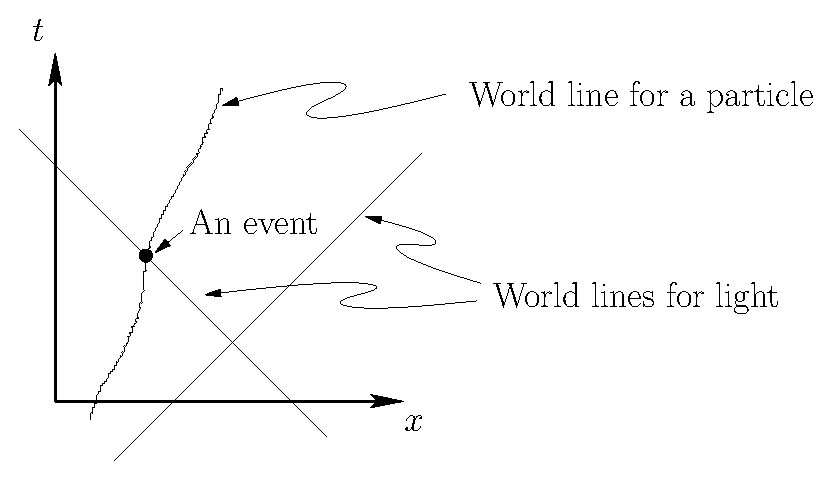
\includegraphics[width=3.5in]{relativistic_spacetime/spacetime1.eps}
\end{center}
\caption{A spacetime diagram with three world lines.  The two world lines for 
light have slopes $+1$ and $-1$.}
\label{fig:spacetime-example}
\end{figure}

Let's use a spacetime diagram to display the world lines of the
three-clock thought experiment of Ch.~\ref{chapter:relativityI},
Section~\ref{section:time-dilation} (see Fig.~\ref{fig:light-clocks}
from that section and Fig.~\ref{fig:worldlines1} in this section).
For example, put clock A at rest at $x = 0$ and clock B at rest at $x
= 0.60\units{lt-s}$.  The world lines for the stationary clocks A
and B are then vertical lines at $x = 0\units{lt-s}$ and $x =
0.60\units{lt-s}$.  Let clock C travel with speed $0.60c$ in the
positive $x$-direction.  Because $c = 1\units{lt-s/s}$, clock C
passes through $x = 0$ at time $t = 0\units{s}$, and it passes
through $x = 0.60\units{lt-s}$ at time $t = 1.0\units{s}$.  It has 
traveled a distance of $0.60\units{lt-s}$ in a time $1.0\units{s}$.
    
Notice in Fig.~\ref{fig:worldlines1} that we have labeled the world
line of clock C as the $t^\prime$ axis.  This is a general result: the
world line of a particular observer (say, someone traveling in a space
ship) is the $t^\prime$ axis for that observer.  This can be
understood by considering a person on a spaceship holding a ball. The
world line for the ball is the same as the world line of the ship and
person since they are all moving together.  From the perspective of
the astronaut, the ball remains right in front of him and isn't moving
anywhere, so it makes sense that that astronaut will say that the
location of the ball remains at $x^\prime = 0$.  And just as it is
true that the points where $x = 0$ in the unprimed frame define the
$t$-axis, so it is that the points where $x^\prime = 0$ in the primed
frame define the $t^\prime$-axis.
    
\begin{figure}[tbp]
\begin{center}
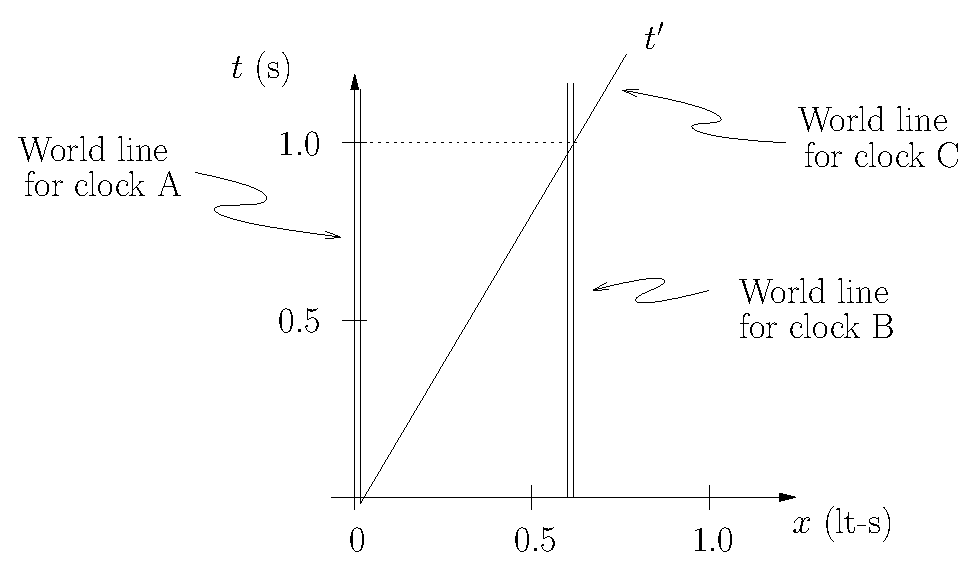
\includegraphics[width=4in]{relativistic_spacetime/worldlines1.eps}
\end{center}
\caption{World lines for the three clocks in the thought experiment
of Section~\ref{section:worldlines}}
\label{fig:worldlines1}
\end{figure}

Some comments are in order:
\begin{enumerate}
\item A world line is nothing more than a plot of time versus
position.  If you ever find yourself stumped about how to plot a
world-line, ask yourself: ``Where is the (whatever) at time $t=0$
(i.e., what is its initial $x$-coordinate)?  Where is it at time 
$t=1$?  At time $t=2$?  \dots''  Then simply plot those points 
and connect them.
\item The slope of a world line is simply $1/v$.  This comes from the
  standard relation: distance = speed $\times$ time, or equivalently, 
  $\Delta x= v \Delta t$.   So $\Delta t =
  \frac{1}{v}\Delta x$.  Practically, this means that if you have a ship
  moving at a speed of, say, $0.5c$, then the slope will be $1/ v$ or
  $2.0\units{s/lt-s}$.  When plotting a world line, this means that
  you go up 2 and over 1 (or over 0.5 and up 1).
\item Don't {\bf ever} forget --- nothing can travel faster than
light, so there should {\bf never} be a world line on a spacetime diagram
 with a
slope whose magnitude is less than 1.  
\item Remember: events are plotted as dots.
\item Label everything clearly.
\end{enumerate}

\begin{figure}[tbp]
\begin{center}
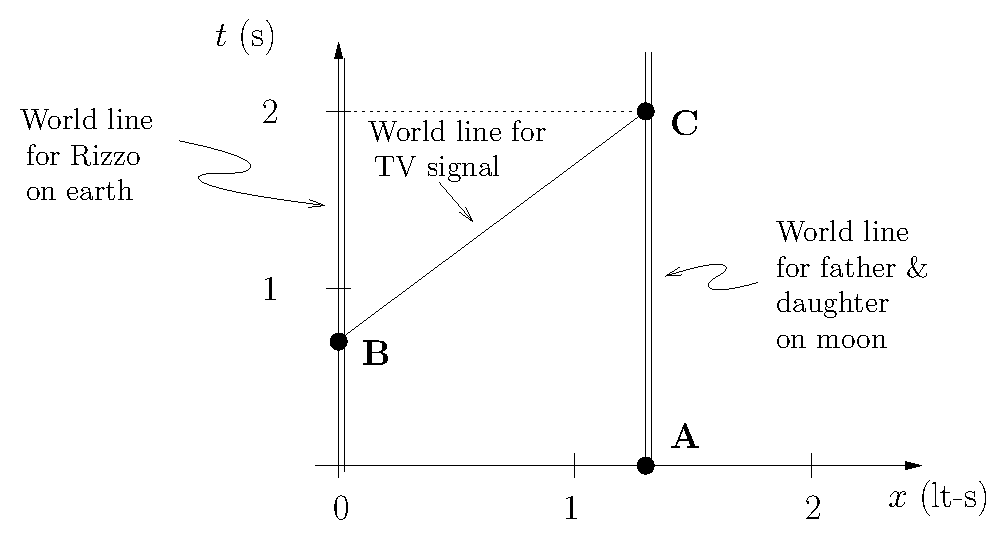
\includegraphics[width=4.2in]{relativistic_spacetime/worldlines2.eps}
\caption{Spacetime diagram for situation discussed in
  Examples~\ref{example:causality-intervals} and
  \ref{example:causality-intervals-diagram}}
\end{center}
\end{figure}

\begin{example}{Spacetime diagram corresponding to 
Example~\ref{example:causality-intervals}} Draw the spacetime diagram
  for the baseball scenario (Cubs losing the World Series) discussed
  in Example \ref{example:causality-intervals}, using the reference
  frame of the Earth/Moon.  Show the world lines for Anthony Rizzo, Jr.,
  the girl and her father, and the TV signal.  Also, show and label
  the following events: A --- girl sneezes, B --- Rizzo strikes out, and
  C --- girl and father see Rizzo striking out.  \solution The world
  lines for Rizzo and the girl/father are simply straight vertical lines
  since they aren't moving in the Earth-Moon reference frame.  If this
  isn't clear, then answer these questions: If we put the Earth at $x
  = 0$ at time $t = 0$, where is the Earth at time $t=1\units{s}$?
  Answer: still at $x = 0$.  At $t=2\units{s}$?  Answer: still at $x =
  0$.  The Earth's world line is nothing more that a set of points
  where $x$ is always zero.  As for the girl/father on the Moon, we
  already said in Example \ref{example:causality-intervals} that they
  are about $1.3\units{lt-s}$ away from the Earth.

We know from the problem that the girl/father see the strikeout
$2\units{s}$ after she sneezes.  So, if she sneezes at $t = 0$ (it is
arbitrary as to what we choose as the $t = 0$ time), then the TV
signal arrives at $t = 2\units{s}$.  It must have been sent from the
Earth at an earlier time, and since it travels at the speed of light,
then the world line for the TV signal is a $45^\circ$ line.  The only
thing left is to plot the three dots for the events.

Note that if you imagine a line between A and B, that line would 
have a slope with magnitude less than 1 (i.e., too shallow), 
indicating that nothing can travel between these two events, 
consistent with the result in Example 1 that the interval is space-like 
and the corresponding events can't be causally linked.
\label{example:causality-intervals-diagram}
\end{example}


\section[the relativity of simultaneity]{Ordering of events --- the 
relativity of simultaneity}

Every event has a set of space and time coordinates.  In Example
\ref{example:causality-intervals-diagram} above, we would say that the
event A (girl sneezes) occurs at time $t=0$ and location $x =
1.3\units{lt-s}$.  Similarly, we can determine the location and times
of events B and C, all as measured by observers in the Earth-Moon
reference frame. Let's add one more event to the scenario: let's say
that at time $t=0$, the pitcher Masahiro Tanaka, Jr., pitches the ball
toward Castro.  In Fig.~\ref{fig:father-daughter} we have added this event and
labeled it P.  In the Earth-Moon frame, we can say quite definitively
that A and P are simultaneous and come first, then B, then C.  Also, A
and C happen at the same location, and P and B happen at the same
location.

\begin{figure}[tbp]
\begin{center}
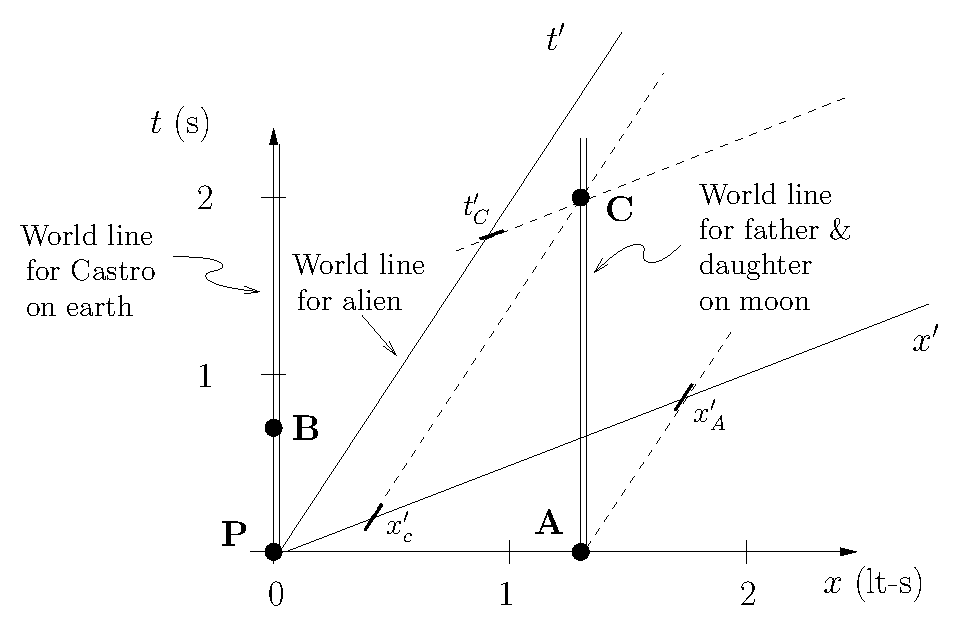
\includegraphics[width=4.3in]{relativistic_spacetime/worldlines3.eps}
\end{center}
\caption{Extension of spacetime diagram in Example
\ref{example:causality-intervals-diagram}.}
\label{fig:father-daughter}
\end{figure}
    
Special relativity helps us answer the following question: how does an
observer moving in a different reference frame view these same events?  We
won't worry here about the actual numerical values of $x^\prime$ and
$t^\prime$ (the position and time as measured by a different observer), but
we can say quite a lot about the ordering of events in space and time
by looking at the spacetime diagrams.


We have added another world line to Fig.~\ref{fig:father-daughter},
namely, the world line for a hypothetical alien whizzing past the
Earth just as the pitch is thrown.  This alien is monitoring the game
to try to understand human culture.  We assume the alien is traveling
at a speed $0.5c$; hence, the world line has a slope of 2.

We have already commented that the world line of an observer in a
primed frame is simply the $t^\prime$ axis for that frame, so we have
labeled the alien's world line $t^\prime$. But where should we put the
$x^\prime$-axis and what scale should we put on it?  It turns out that to
satisfy the invariance of the speed of light, we must draw the
$x^\prime$-axis at the same angle relative to the $x$-axis as the angle of
the $t^\prime$-axis relative to the $t$-axis. This means the slope of the
$x^\prime$-axis is equal to the speed $v$ of the primed frame relative to the
unprimed frame.
    
Recall that the $t^\prime$-axis represents points where $x^\prime =
0$.  It turns out that $x^\prime$ is constant along any line parallel
to the $t^\prime$-axis.  In other words, lines parallel to the $t^\prime$-axis
are equal-location lines for the primed frame of reference, just as
the $t$-axis and all lines parallel to it are each lines of equal
location for the unprimed frame of reference.  The same ideas work for
events on lines parallel to the $x$ or $x^\prime$ axes; events on a line
parallel to the $x$-axis are simultaneous in the unprimed frame, and
events on a line parallel to the $x^\prime$-axis are simultaneous in the
primed reference frame.
    
We can use these ideas to ``read off'' coordinates for events in
both reference frames.  As an example, let's look at event C in
Fig.~\ref{fig:father-daughter}.  We have already commented that in the
unprimed frame, its $x$ location is $1.3\units{lt-s}$ and its time
is $2\units{s}$.  The coordinates of this event in the alien's
reference frame are determined by drawing lines parallel to the
$x^\prime$ and $t^\prime$ axes (shown as dotted lines in
Fig.~\ref{fig:father-daughter}).  The intersections of these
construction lines with the opposing primed axis gives the $x_C$ and
$t_C$ coordinates. The rules for determining coordinates can be
summarized as follows:
\begin{enumerate}
\item To find $x_C$, draw a straight line through C parallel to the
$t$-axis and read off where it crosses the $x$-axis.  
\item To find $t_C$ draw a straight line through C parallel to the
$x$-axis and read off where it crosses the $t$-axis.  
\item To find $x_C^\prime$, draw a straight line through C parallel to
the $t^\prime$-axis and read off where it crosses the $x^\prime$-axis.
\item To find $t_C^\prime$, draw a straight line through C parallel to the
$x^\prime$-axis and read off where it crosses the $t^\prime$-axis.
\end{enumerate}

Using this type of construction, we can see that although events A and
C occur at the same place in the unprimed (Earth-Moon) reference
frame, event C happens to the left of the event A in the primed
(alien) reference frame.  This is easy to understand: the alien is far
from the Moon when event A happens, so A is far ``to the right,''
whereas the alien is close to the Moon when event C happens, so from
the alien's perspective, C isn't so far to the right, i.e.,
smaller $x^\prime$ coordinate.
    
    But what about the ordering of events in time?  We have commented
that the invariance of the spacetime interval says that if two
observers disagree about distances, then they will have to disagree
about time intervals as well.
    
\begin{boxittext}
{{\bf In preparation for class:} Look at the $t^\prime$ coordinates for events
P and A.  In the Earth-Moon reference frame, these events are simultaneous.
What about in the alien reference frame?
}
\end{boxittext}

We have said that any two events on a line parallel to the
$x^\prime$-axis are simultaneous in the primed frame of reference.
Similarly two events that lie on a line parallel to the $x$-axis are
simultaneous in the unprimed frame.  However two different events
cannot lie both on a line parallel to the $x$-axis and parallel to the
$x^\prime$-axis.  Thus two events that are simultaneous in one frame cannot
be simultaneous in the other frame.  We explore this idea in the
following example.

\begin{example}{Simultaneity is Relative}  
Einstein showed, with the following thought experiment, that two events
which occur at the same time but at different places in one frame,
occur at different times in another frame.

\begin{figure}[tbp]
\begin{center}
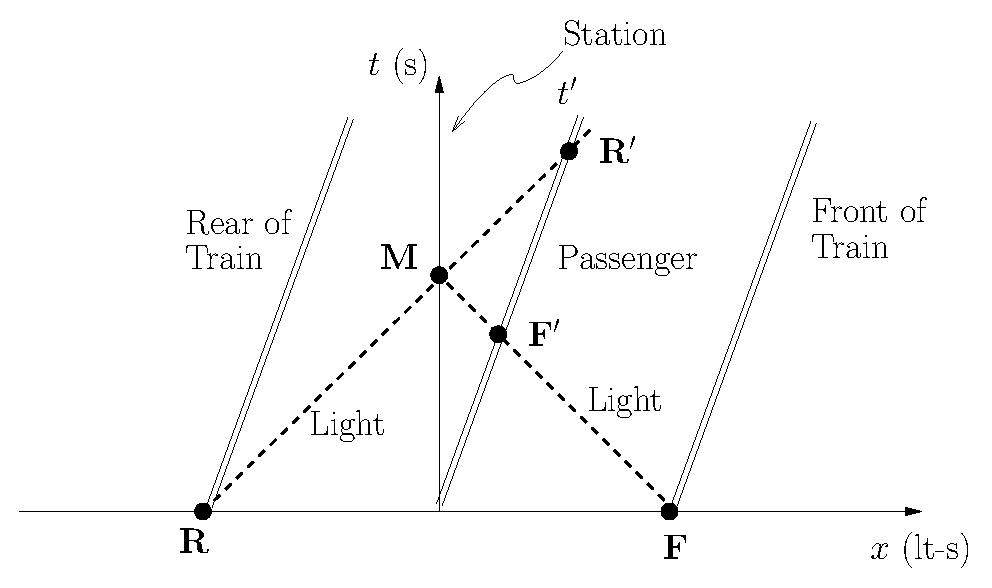
\includegraphics[width=4.2in]{relativistic_spacetime/worldlines4.eps}
\end{center}
\caption{Spacetime diagram for train of Example 
\ref{example:simultaneity}. (Light
world lines shown as dashed lines.)}
\label{fig:simultaneity}
\end{figure}

Imagine a train moving past a station.  By chance, lightning
happens to strike the front and back of the train at the same time
according to observers on the station platform.  Light pulses from
these strikes travel toward the middle of the train, where a passenger
observes their times of arrival.  Do the light pulses arrive
simultaneously or does one arrive before the other, and if so, which
one?
\solution
Use a spacetime diagram, Fig.~\ref{fig:simultaneity}, with the
station at rest in the unprimed frame and the train at rest in the
primed frame.  The $x$- and $x^\prime$-axes both lie along the track.
(Note:  this does {\bf not} mean that the $x$- and $x^\prime$-axes
are the same thing on a spacetime plot.  The $x^\prime$-axis is not
shown in Fig.~\ref{fig:simultaneity}, but remember that it is the mirror
image of the $t^\prime$-axis about a $45^\circ$ line; i.e., the angle
between the $t$- and $t^\prime$-axes is the same as the angle between
the $x$- and $x^\prime$-axes.)
The world line for the middle of the station is shown as the $t$-axis.

Because all parts of the train are at rest in the primed frame, we
draw the world lines for the front and the rear ends of the train
parallel to the $t^\prime$-axis.  Also, in
Fig.~\ref{fig:simultaneity}, we have chosen the world line for the
passenger riding in the exact middle of the train to be the
$t^\prime$-axis.  In the primed frame the front and rear world lines
are then equidistant from the passenger, by definition.

The lightning strikes occur at points R and F on the world lines of 
the rear and front of the train.  Because each strike represents an 
event and because these two events occur simultaneously in the 
station frame, R and F must be drawn on the same horizontal line.  
We arbitrarily choose this line to be at $t = 0$.

The light pulses produced by the lightning strikes travel with speed
$c = 1\units{lt-whatever per whatever}$ from the event F back toward
the passenger and from R forward toward the passenger.  The pulse from
F is represented by a world line of slope $-1$ and the pulse from R is
represented by a world line of slope $+1$.  Figure
\ref{fig:simultaneity} shows that the pulse from F arrives at the
passenger's world line (at F$^\prime$) earlier (i.e., at a smaller
value of $t^\prime$) than does the pulse from R, which arrives at
R$^\prime$.

The passenger must conclude that the front strike occurred before 
the rear strike because she is sitting in the middle of the train, 
equidistant from R and F, and she knows the light pulses must have 
taken the same time (in her frame) to reach her.  By the same 
argument, an observer on the station platform who was at the exact 
middle of the train at $t = 0$ when the strikes occurred, sees the 
pulses at the same time.  This is shown on the spacetime diagram 
by the fact that the world lines of the pulses cross the world line of 
the middle of the station at $x = 0$ (event M) at the same time.
\label{example:simultaneity}
\end{example}

\newpage

\section*{Problems}
\markright{PROBLEMS}

\begin{problem}
If two events are separated by a time-like interval in one
frame of reference, are they separated by a time-like interval in all
frames of reference?  Explain.
\end{problem}

\begin{problem}
A simple way of synchronizing two clocks at rest relative to one
another is to stand exactly halfway between them and emit light pulses
toward each of them at the same instant of time.  Each clock is then
set to 0 when the synchronizing pulse reaches it.
  \begin{enumerate}
  \item How does this scheme ensure that the clocks are started
    simultaneously?  
  \item On a spacetime diagram show the world lines of two
    clocks at rest in the unprimed frame of reference at $x = 0$ and at $x =
    L$, along with the world lines of two synchronizing light pulses that
    start from the midpoint and reach each of the two clocks at $t = 0.$
  \end{enumerate}
\label{prob:synchronizeB}
\end{problem}

\begin{problem}
  Events A, B, and C are shown on the spacetime diagram in
  Fig.~\ref{fig:spacetimeI}.
  \begin{figure}[h]
  \begin{center}
    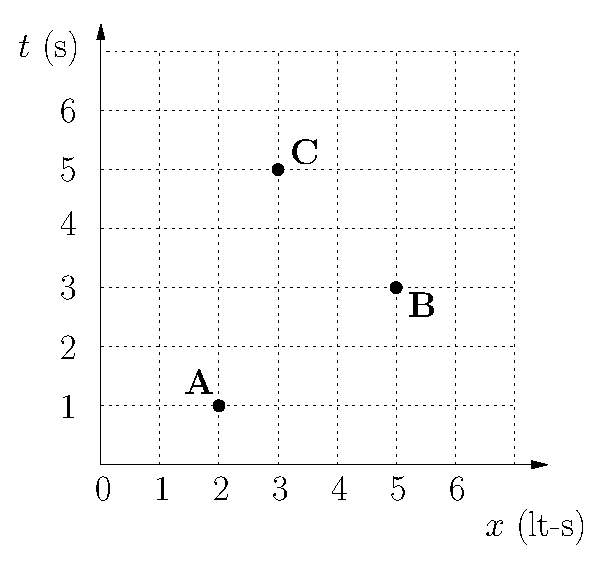
\includegraphics[width=2.8in]{relativistic_spacetime/p_spacetimeI.eps}
  \caption{Figure for Problem \ref{prob:spacetimeI}.}
  \label{fig:spacetimeI}
  \end{center}
  \end{figure}
  \begin{enumerate}
  \item Calculate the value of the squared interval for each pair of
    events, i.e., find $I^2_{AB}$, $I^2_{AC}$, and $I^2_{BC}$.  
  \item Label each interval as time-like, space-like, or light-like.  
  \item In the frame shown, event A occurs before B, which occurs before
    C.  Which pairs of events could have their time-order reversed
    (switching before and after) by choosing an appropriate reference
    frame?  
  \item In the frame shown, event B occurs to the right of C, which
    occurs to the right of A.  Which pairs of events could have their
    space-order reversed (switching left and right) by choosing an
    appropriate reference frame?  
  \item Which events could be a ``cause'' for which other events?
  \end{enumerate}
\label{prob:spacetimeI}
\end{problem}

\begin{problem}
Fig.~\ref{fig:spacetimeII} shows a spacetime diagram with seven straight lines
through the origin labeled with capital letters A through G.  Various
events are marked as points with small letters a through e.  The $x$-$t$
axes belong to the Earth's reference frame.

\begin{figure}[htbp]
\begin{center}
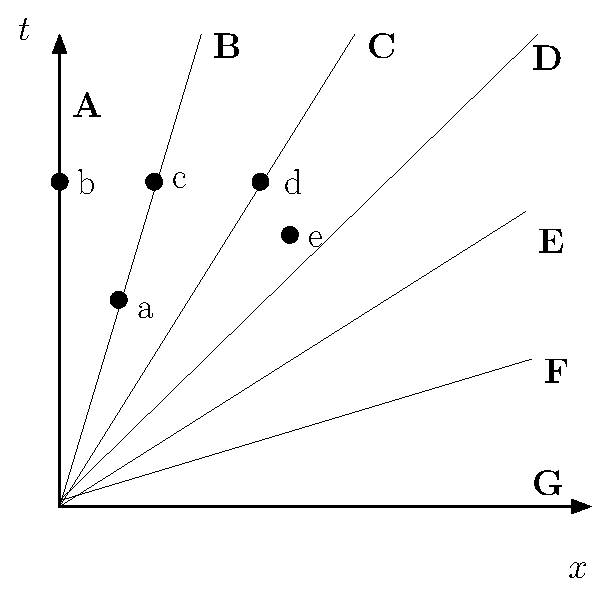
\includegraphics[width=2.5in]{relativistic_spacetime/p_spacetimeII}
\caption{Figure for Problem \ref{prob:spacetimeII}.}
\label{fig:spacetimeII}
\end{center}
\end{figure}
 
\begin{enumerate}
\item Which line is a world line of an object at rest relative to the Earth?
\item Which line is a world line of a spaceship traveling at speed  
$+0.3c$ relative to the Earth?
\item Which line is a world line of a light pulse emitted by the
spaceship as it passes the Earth? 
\item Which events happen simultaneously in the Earth frame?  
\item  Which events happen simultaneously in the spaceship frame?  
\item Which pairs of events are clearly separated by space-like
intervals?  Which are clearly separated by time-like intervals?
\end{enumerate}
\label{prob:spacetimeII}
\end{problem}

\begin{problem}
For Example \ref{example:simultaneity} in the text, show from
the spacetime diagram in Fig.~\ref{fig:simultaneity} that lightning
hit the front of the train at a negative value of $t^\prime$, but that
lightning hit the rear of the train at a positive value of $t^\prime$.
Use the rule for finding the $t^\prime$ coordinate of an event to
solve this problem.  [Hint: you might want to extend some of the axes
in the negative direction.]  
\end{problem}

\begin{problem}
Farmer Brown, at rest in his frame, carries a ladder through
a barn.  According to Farmer Brown, the ladder measures
$20\units{lt-ns}$.  According to observers at rest with respect
to the barn, Farmer Brown and his ladder are moving at a
speed $0.80c$ (alternately, Farmer Brown sees the barn 
moving at speed $0.80c$).  In the barn's frame, the
front door of the barn is at $x = 0 \units{lt-ns}$ and the back 
door is at $x = 16\units{lt-ns}$.
\begin{enumerate}
\item Calculate the length of the ladder as measured by
observers in the barn's reference frame.  According to
these observers, will the ladder fit within the barn?
\item Calculate the length of the barn as measured by
Farmer Brown.  According to Farmer Brown, will the ladder
fit within the barn?
\item Draw a careful spacetime plot for this situation,
with appropriate tick marks on the axes (labeled with
numbers).  Starting with the barn frame, draw world
lines for the entrance and exit of the barn (i.e., the
front and back doors).  Draw also world lines for the front and
back of the ladder (which is moving as viewed in the
barn frame).  The distance between the front and back of
the ladder in your plot should agree with your answer
to part (a), and the slopes of these lines should be
consistent with the known velocities.
\item Label the following events on your diagram:
A = front of ladder enters the barn; B = front of ladder
leaves the barn; C = back of ladder enters barn;
D = back of ladder leaves barn.  Determine the order
of these events in time as viewed from the barn's
reference frame.  Is this result consistent with your
answer to (a), i.e., whether or not the ladder fits in the
barn, according to barn-frame observers?  (Consider
whether the back of the ladder enters the barn before
or after the front of the ladder leaves the barn.)
\item Determine the order of events A, B, C and D as
viewed from Farmer Brown's reference frame.  Is this
result consistent with your answers to (b)?
\item Based on your answers for this problem, can you
see how relativistic time-ordering (i.e, the fact that
different observers do not necessarily agree on the
ordering of events in time) is necessarily linked with
length contraction?
\end{enumerate}
\label{prob:farmer}
\end{problem}

\newpage
\begin{figure}[!h]
\[ 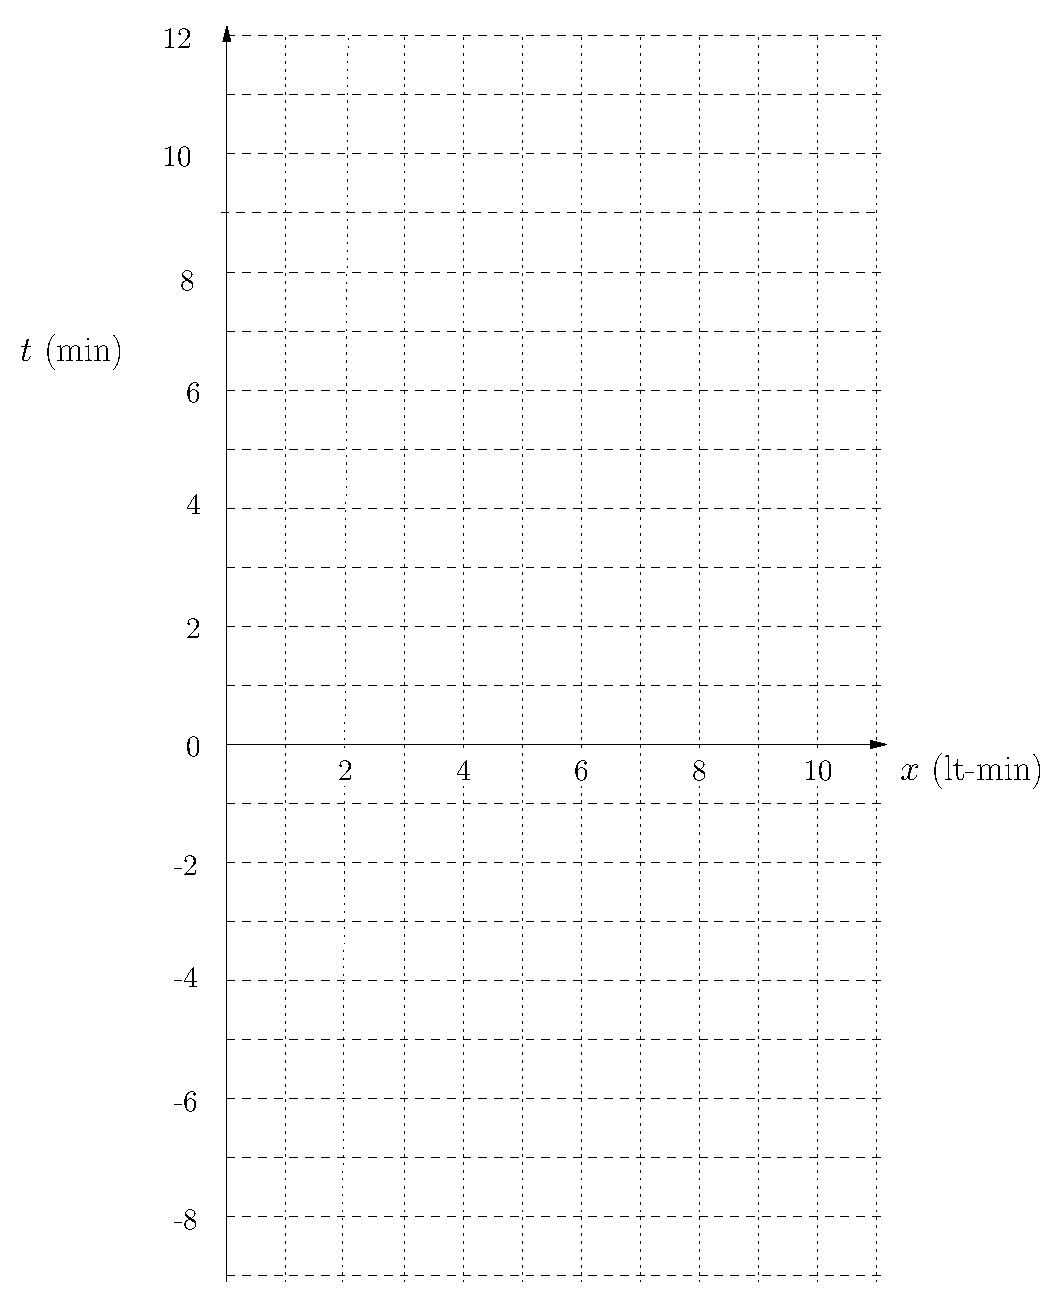
\includegraphics[width=5.5in]{relativistic_spacetime/p_solar_flare.eps} \]
\caption{Figure for Problem \ref{prob:solar_flare}.}
\end{figure}

\newpage

\begin{problem}
The Earth is $8\units{lt-min}$ from the Sun.  An astronomer on Earth,
looking through a telescope, notices the sudden appearance of a giant
solar flare on the Sun's surface.  At precisely that instant (when the
astronomer detects the flare), a Klingon space ship whizzes over his
head at speed $0.8c$, heading straight for the Sun.
\begin{enumerate}
\item On the facing page, construct a spacetime diagram for this situation.  
  Label the following three events: {\bf A}: Klingon ship hits Sun, 
  {\bf B}:  flare occurs on Sun, and {\bf C}: Klingon ship passes Earth.  
  (Note that event B is the occurrence of the flare {\em on\/} the Sun, 
  not the detection of the flare by an astronomer on Earth.)
\item Order the events A, B, C, from earliest to latest, according to
  Earth-based observers.
\item Calculate the time intervals $\Delta t$ between each pair of
  events (AB, AC, and BC), according to Earth observers.
\item Calculate the interval $\Delta t^\prime_{BA}$ between events B
  and A, but now according to Klingon ship observers.
\item Classify each of the intervals as space-like, time-like or
  light-like.
\end{enumerate}
\label{prob:solar_flare}
\end{problem}

% \begin{problem}
% A cosmic ray particle moving down toward Earth at speed $0.99c$ decays
% $2.0\units{$\mu$s}$ after it was produced as measured in the frame in
% which the particle is at rest.
% \begin{enumerate}
% \item Represent the birth and decay of the particle on a spacetime
%   diagram.
% \item In the cosmic ray's rest frame the Earth is moving toward it.
%   In this frame, how far, in light-$\mu$s, did the Earth travel during
%   the particle's lifetime?
% \item Observers in the Earth's frame see the particle coming down
%   toward Earth.  How long did the particle live according to these
%  observers and how far did it travel?
% \end{enumerate}
% \label{prob:cosmic_ray}
% \end{problem}

\begin{problem}
Two spacecraft, {\em Aaaak} and {\em Blech}, are carrying aliens from 
the planet Zortox to Earth.  Both spacecraft are traveling
at a speed of $0.6c$ relative to the Earth, with {\em Aaaak} in
front.  In the Earth's frame, {\em Aaaak} and {\em Blech} are
a distance $8.0\units{lt-s}$ apart. 
At the moment that {\em Aaaak} passes Earth, the Zortoxians aboard {\em Aaaak} 
dump its garbage.  At a time $10.0\units{s}$ later 
(as measured by earthlings) {\em Blech} dumps its garbage.  
\begin{enumerate}
\item Draw a spacetime diagram in Earth's frame that includes 
worldlines for Earth, {\em Aaaak}, and {\em Blech}.  Indicate and label 
the events corresponding to the garbage dumps.
\item How far has {\em Blech} traveled during the $10.0\units{s}$ 
between the two garbage dumps measured by earthlings?
\item What is the distance between the two garbage dump events measured by 
earthlings?
\item What is the distance between the two garbage dump events 
measured by the Zortoxians on board their ship?
\item Calculate the time interval between garbage dump events measured by 
the Zortoxians on board their ship.
\end{enumerate}
\label{prob:two_ships}
\end{problem}

%\begin{problem}
%Two spacecraft ({\em Aaaak} and {\em Blech}) carrying aliens from 
%the planet Zortox are traveling toward  Earth (with {\em Aaaak} in front) 
%at a speed of $0.6c$ relative to the Earth.  In the Earth's frame of 
%reference {\em Aaaak} and {\em Blech} are $8.0\units{lt-s}$ apart. 
%At the moment they pass Earth, the Zortoxians aboard {\em Aaaak} 
%dump its garbage, and $10.0\units{s}$ later 
%(as measured by earthlings) {\em Blech} dumps its garbage.  
%\begin{enumerate}
%\item Draw a spacetime diagram in Earth's frame that includes 
%worldlines for Earth, {\em Aaaak}, and {\em Blech}.  Indicate and label 
%the events corresponding to the garbage dumps.
%\item How far has {\em Blech} traveled during the $10.0\units{s}$ 
%between the two garbage dumps measured by earthlings?
%\item What is the distance between the two garbage dump events measured by 
%earthlings?
%\item What is the distance between the two garbage dump events 
%measured by the Zortoxians on board their ship?
%\item Calculate the time interval between garbage dump events measured by 
%the Zortoxians on board their ship.
%\end{enumerate}
%\label{prob:two_ships}
%\end{problem}


\newpage

\begin{problem}
A train of rest length $40\units{lt-ns}$ moves along the
tracks at $0.8c$ and is struck by two lightning bolts.  One bolt hits
the front of the train and the other hits the back.  According to
observers  on the tracks the bolts are simultaneous.
\begin{enumerate}
\item How far apart did the lightning bolts strike according to 
observers on the tracks?  
\item According to riders on the train, how much time passed between the
striking of the lightning bolts?  
\item According to riders on the train, which lightning bolt 
struck first? 
\end{enumerate}
\end{problem}

\begin{problem}
Joe holds and lights a sparkler, and one minute later, it goes
out.  Cheri, riding in a rocket past these events, notes that, as
measured in her frame, the sparkler burned for 100 seconds.
\begin{enumerate}
\item How far apart in Cheri's frame did these two events (lighting
and going out) occur? 
\item As measured by Cheri, how far did the lit sparkler travel, and
how fast was it moving?  
\item As measured by Joe, how fast was Cheri traveling during the one
minute of sparkler light, and how far did she travel?
\end{enumerate}
\label{prob:sparkler}
\end{problem}

\newpage

\begin{problem}
The spacetime diagram in the figure shows the world lines of the Earth,
a star, and a rocket, as well as several labeled events.
\begin{figure}[!h]
\begin{center}
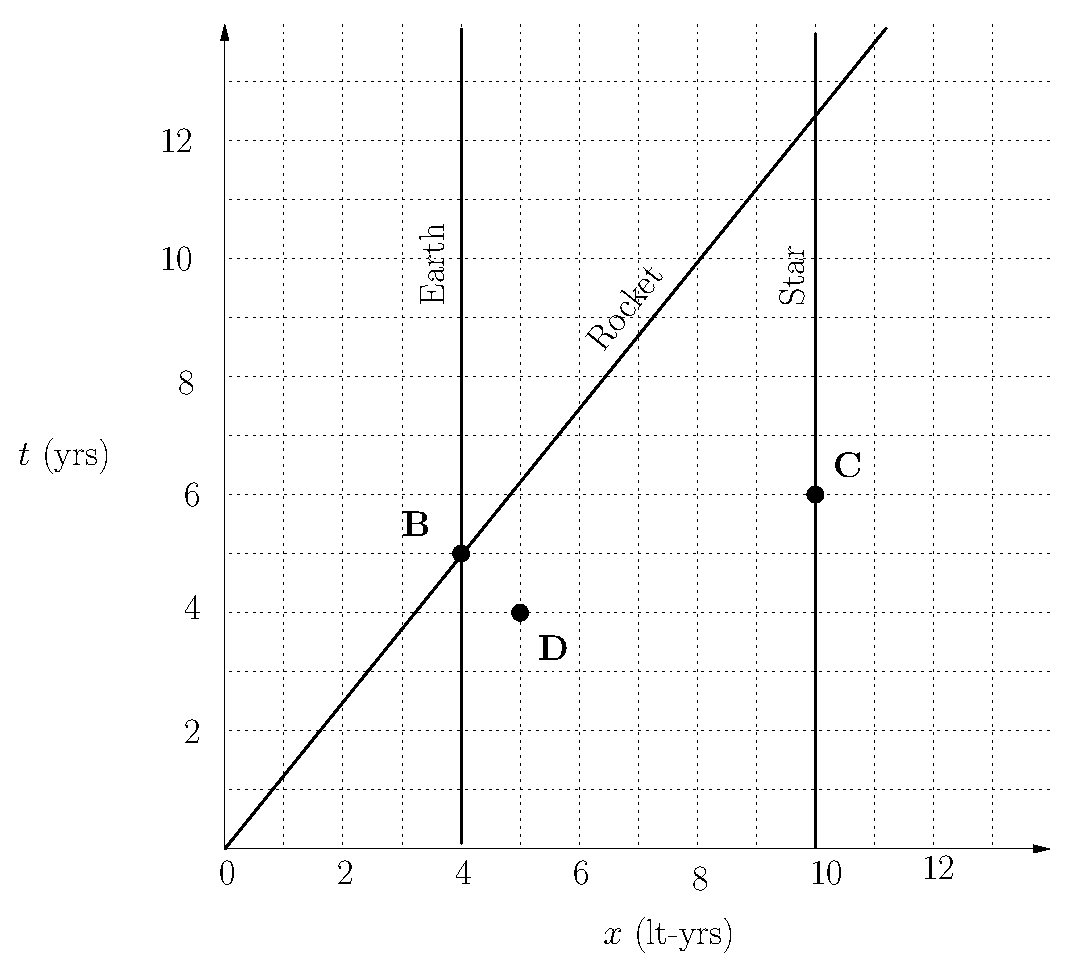
\includegraphics[width=3.68in]{relativistic_spacetime/p_spacetimeIII.eps}
\end{center}
\caption{Figure for Problem \ref{prob:spacetimeIII}.}
\end{figure} 
\begin{enumerate}
\item On the diagram, label as ``A'' the event ``Rocket arrives
at Star.''
\item Determine the speed of the Rocket, as measured by Earth
observers.
\item Determine the time between passing the Earth and passing the
Star, as measured by Rocket observers.
\item Determine the distance between the Earth and the Star, as
measured by Rocket observers.
\item Draw the world line of a lost satellite passing the Earth at the
same time as the Rocket, but going away from the Star at a speed that
is $\frac{1}{2}$ of the Rocket speed (as determined by Earth
observers.)  Label this line ``Satellite.''
%\item Determine the speed of the satellite as measured by Rocket observers.
%This part removed in 2011 when velocity transformations moved to mom/energy
%chapter.
\item Order the events A, B, C, D, from earliest to latest, as
observed in the Earth-Star reference frame.
\item Order the events A, B, C, D, from earliest to latest, as
observed in the Rocket reference frame.  
\item In some reference frame, the events C and D are simultaneous.
In that frame, what is the distance between events C and D?
\item Explain why no one could ever measure the proper time between
events C and D.  
\end{enumerate}
\label{prob:spacetimeIII}
\end{problem}


%\chapter{Relativistic Momentum and Energy}
\label{chapter:relativity_pande}


%\section*{Objectives}
%\begin{objectives}
%\item Know the modifications in the definitions of momentum and energy
% needed to maintain invariance of the conservation laws.
%%\item Show that $E^2- p^2c^2$ is a constant, related to a particle's
%%mass and independent of velocity.  
%\item Given any two of a particle's dynamical quantities ($p$, $E$, $u$, $K$,
%and $m$) determine any of the others.  
%\item Specialize any of the equations relating $p$, $E$, $u$, $K$, and $m$ to
%zero-mass particles.
%\end{objectives}

\section{Introduction}

So far in our discussions of relativity, we have taken a very simple
principle --- the {\em Principle of Relativity}, which states that the
laws of physics are the same for observers in any inertial reference
frame --- and have used this principle to change completely our notions
of how time and space work.  But we are not yet done looking at the
implications of this principle.  It will be necessary to generalize
the classical relations for energy and momentum to account for the
strange behavior that we have already seen at relativistic velocities.
And the new relativistic equations for energy and momentum carry
significant implications that change our notions of energy and matter.
This discussion leads to what is probably the most famous equation in
all of physics --- namely $E = mc^2$ --- as well as the basic principle
behind nuclear power generation.  Of course, this is also the principle 
behind nuclear weapons, so it can be argued that this result fundamentally
changed society.  But this is also the principle behind energy generation
in stars (including our own Sun); there would be no life on this planet
without this principle.
% As we will see, we will also find a new invariant in this discussion;
% namely, the combination $E^2 - p^2c^2$.

But before we discuss relativistic energy and momentum, we will take
a closer look at the concept of velocity.  If observers in different
reference frames don't agree on the results of measurement of lengths 
and time intervals, they won't agree on the results of their determinations
of velocities. 


\section{Relativistic Velocity Transformations}

Let's say that two spaceships leave Earth.  The {\em USS Zaphod}
leaves the Earth going in one direction with a speed $0.8c$ relative
to Earth.  The {\em USS Beeblebrox} leaves Earth going in the opposite
direction with a speed $0.8c$ relative to Earth.  What is the speed
of the {\em Zaphod} from the reference frame of the {\em Beeblebrox}?
Based on classical assumptions, you might expect the answer to be
$1.6c$.  But this conflicts with Einstein's theory of relativity which
states that no object can travel faster than the speed of light
relative to any other observer.  It is clear that it is necessary to
replace classical laws for addition and subtraction of velocities with
a more general, relativistic transformation.

A relativistic approach to velocity addition and subtraction was already
hinted at earlier in Chapter \ref{chapter:relativityI}.  The principle
of invariance of the speed of light requires that all observers (in
any reference frame) measure the same speed for a pulse of light ---
we can't simply add and subtract velocities.  On the other hand, common
experience shows us that for non-relativistic speeds, simple addition
and subtraction work fine.  So, we need a velocity transformation
relation that reduces to the classical result for small speeds, but
which prevents anything from traveling faster than the speed of light.
It turns out that this can be accomplished by taking the classical result
and dividing by a relativistic correction that becomes significant (i.e.,
not just 1) for speeds close to $c$.

Figure \ref{fig:rel1_vtransform} shows the scenario that we are
discussing.  Two reference frames are defined: an unprimed frame
denoted by observer A and a primed frame denoted by observer B on a
spaceship moving with a speed $v$ relative to observer A.  They are both
measuring the speed of the same object.  Observer A says the object is
moving with a speed $u_{\rm obj}$ while observer B says the ball is
moving with a speed $u_{\rm obj}^\prime$.

\begin{figure}[tbp]
\begin{center}
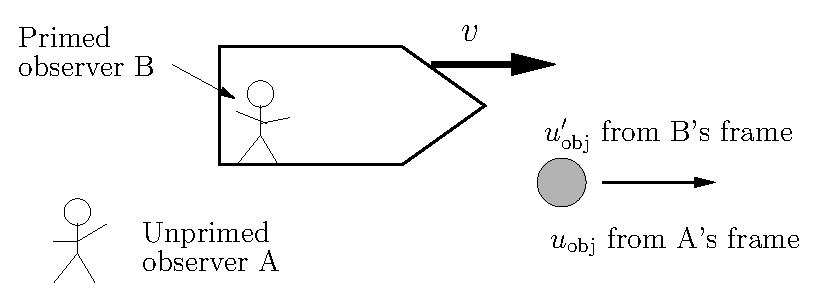
\includegraphics[width=4in]{basic_postulates_of_relativity/rel1_vtransform.eps}
\end{center}
\caption{An object moving in the $x$-direction relative to both
unprimed and primed frames.  The speed of the object is measured to be
$u_{\rm obj}$ from the reference frame of observer A and 
$u_{\rm obj}^\prime$ from the reference frame of observer~B.}
\label{fig:rel1_vtransform}
\end{figure}   

The question is: How are $u_{\rm obj}$, $u^\prime_{\rm obj}$ and $v$ related?
The answer is given by a {\em velocity transformation} equation,

\begin{boxiteq}
{\begin{equation}
u_{\rm obj} = \frac{u_{\rm obj}^\prime + v}{1 + u_{\rm obj}^\prime v/c^2}.
\label{eq:vtransform}
\end{equation}}
\end{boxiteq}
                                                
\noindent Equation (\ref{eq:vtransform}) is used to relate an object's
velocity in one frame to that as viewed in another frame.

We won't derive Eq.~(\ref{eq:vtransform}) rigorously here.  Rather,
note that if the object is a pulse of light, then $u_{\rm obj}^\prime
= c$, and Eq.~(\ref{eq:vtransform}) reduces to
\begin{equation}
u_{\rm obj} = \frac{c+v}{1 + cv/c^2} = \frac{c+v}{1+v/c} = 
c\left(\frac{c+v}{c+v}\right) = c.
\end{equation}
Both observers measure the object to have a speed $c$, so, the
invariance of the speed of light is preserved in this transformation.

Note that the numerator in Eq.~(\ref{eq:vtransform}) is the result
that you would get classically, whereas the denominator is a
relativistic correction. Also, note that if either the object or the
primed observer are traveling at speeds that aren't a significant
fraction of the speed of light, then the denominator of
Eq.~(\ref{eq:vtransform}) is very nearly 1, so we recover the
classical result for ``everyday'' speeds.
    
We'll show how to work with this relation in the next example.

\begin{example}{Baseball velocity addition}
  Bucknell Bison baseball pitcher Christy Mathewson throws a blazing 
  fastball while riding on a really fast train.
  From his reference frame (i.e., the train's frame) the ball moves
  toward the front of the train with a speed $u_{\rm ball} = 0.7c$.
  The train itself is moving relative to the ground with speed $v =
  0.8c$.  How fast is the ball moving relative to someone on the
  ground?  

\solution Classically, the speed as viewed from the ground
  would be $u_{\rm ball} + v$ or $1.5c$.  (This is the numerator of
  Eq.~(\ref{eq:vtransform}).)  But, of course, this isn't possible in
  a relativistic universe where nothing goes faster than $c$.  Using
  Eq.~(\ref{eq:vtransform}) we find
\begin{equation}
  u_{\rm ball} = \frac{u_{\rm ball}^\prime + v}{1+ u_{\rm ball}^\prime v/c^2}
  = \frac{0.7c + 0.8c}{1+0.7\times 0.8} = 0.96c.
\end{equation}
Note that relativistic correction keeps the speed less than $c$.

\noindent {\bf Exercise}: What if the ball were a beam of light?  How
fast would it be moving from the train's reference frame?  How fast
from the ground's reference frame?  Show that
Eq.~(\ref{eq:vtransform}) gives the correct result for this case.
\end{example}

If the problem gives you the speed as measured by the unprimed observer, 
you can use the following inverse transformations to get the speed as
measured by the primed observer:

\begin{boxiteq}
{
\begin{equation}
u_{\rm obj}^\prime = \frac{u_{\rm obj}- v}{1 - u_{\rm obj} v/c^2}.
\label{eq:vtransform-inverse}
\end{equation}
}
\end{boxiteq} 

You don't really need to write down these relations or try to figure
out which speed is $v$, which speed is $u_{\rm obj}$, and which speed
is $u_{\rm obj}^\prime$.  There is a very simple way of handling all
of these problems.  No matter which velocity you are looking for, the
answer is always:
\begin{equation}
\frac{\text{classical result}}{\text{relativistic correction}}, \nonumber 
\end{equation}
where the relativistic correction is simply ``$1+$(product of other two
speeds divided by $c^2$)'' or ``$1-$(product of other two speeds divided
by $c^2$).''.  You will be given two velocities, and you'll be looking
for the third one.  Just figure out the answer classically, then divide
by the correction.  The only question then is whether to use the ``$+$''
or ``$-$'' in the correction.  The rule: if you {\em added} magnitudes of
velocities in the numerator, then you use the ``$+$'' in the denominator,
and if you {\em subtracted} magnitudes in the numerator, then you use the
``$-$'' in the denominator.  This will take care of any velocity addition
or subtraction that you need.

\section{New definitions for energy and momentum}

You have learned previously that in interactions among low velocity
particles in which the only forces are the interparticle forces
(i.e.\ no {\em external} forces), the total momentum $\sum_i
m_i\vec{u}_i$ and the total mass $\sum_i m_i$ are conserved.  (As in
Chapter \ref{chapter:relativistic_spacetime}, we use the symbol $u$ to
refer to the velocity of some particle as viewed from a reference
frame, reserving $v$ for the velocity of the reference frame itself.)
For example, when particle 1 collides with particle 2 and particles 3,
4, and 5 emerge from the point of collision, we have two conservation
laws:
\begin{equation}
\vec{p}_1 +\vec{p}_2 = \vec{p}_3 +\vec{p}_4 +\vec{p}_5
\label{eq:pcons}
\end{equation}
and
\begin{equation}
m_1 + m_2 = m_3 + m_4 + m_5 
   \text{\hspace{0.2in}{\bf Caution: Only valid classically!}}
\label{eq:mcons}
\end{equation}

After Einstein discovered the velocity transformation law,
Eq.~(\ref{eq:vtransform}) and (\ref{eq:vtransform-inverse}), he
recognized that the classical definition of momentum ($\vec{p} =
m\vec{u}$) was incompatible with Eq.~(\ref{eq:pcons}) and the Relativity
Principle.  That is, for a given collision, classical momentum could
be conserved in one frame but not another.  An example will illustrate
this:


\begin{example}{Say goodbye to the classical expression for momentum.}  
\label{ex:momentum-goodbye} 
(For this example, we use the natural units of MeV, MeV/$c$, MeV/$c^2$
and $c$.  More detail on these units appears section
\ref{section:rel-units}.)  Figure \ref{fig:momentum_goodbye} shows a
particle of mass $9\units{MeV/$c^2$}$ and speed $0.8c$ striking a
stationary particle of mass $5 \units{MeV/$c^2$}$, producing a
single particle.  (a) Calculate the mass and speed of the single
particle after the collision.  (b) Show that classical momentum is
{\em not} conserved in the frame in which the final particle is at
rest.
\begin{figure}[tb]
\begin{center}
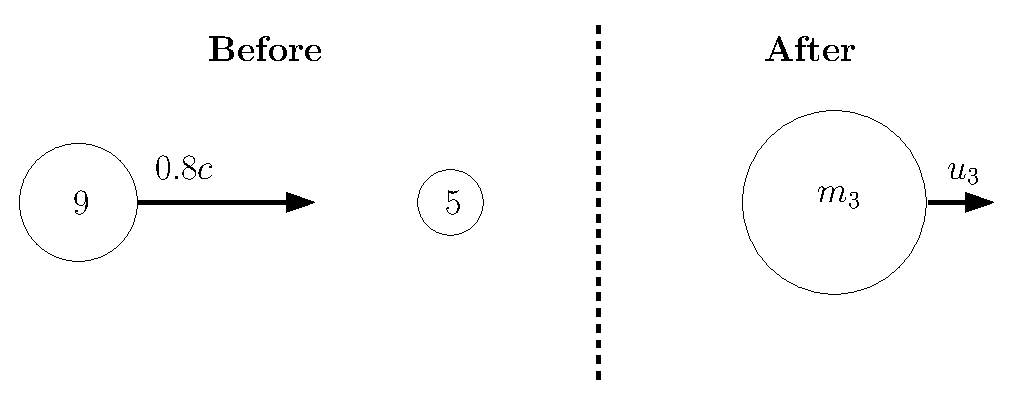
\includegraphics[width=3.8in]{relativistic_momentum_and_energy/relpande1.eps}
\end{center}
\caption{Collision discussed in Example \ref{ex:momentum-goodbye}.
\label{fig:momentum_goodbye}}
\end{figure}
\solution
The classical laws Eqs.~(\ref{eq:pcons}) and (\ref{eq:mcons}) would
yield
\begin{eqnarray}
\text{Eq.~(\ref{eq:pcons})}&\Rightarrow& 9\units{MeV/$c^2$}\times 0.8c + 
                     5\units{MeV/$c^2$}\times 0 = m_3u_3 \nonumber \\
                 &\Rightarrow& u_3 = \frac{7.2\units{MeV/$c$}}
                            {14\units{MeV/$c^2$}} = 0.514c\nonumber
\end{eqnarray}
and 

\begin{eqnarray}
\text{Eq.~(\ref{eq:mcons})}
&\Rightarrow& 9\units{MeV/$c^2$} + 
                     5\units{MeV/$c^2$} = m_3 \nonumber \\
                    &\Rightarrow& m_3 = 14\units{MeV/$c^2$}. \nonumber
\end{eqnarray}

Transform now to a frame in which the final particle is at rest.  This
clearly means that we should view the collision from a spaceship
traveling with particle 3 at $0.514c$ to the right, relative to the
original observer. Equation~(\ref{eq:vtransform-inverse}) gives
\begin{eqnarray}
u_3^\prime &=& \frac{u_3 - v}{1 - u_3v/c^2} = 
              \frac{0.514c - 0.514c}{1-0.514^2} = 0 \nonumber \\
u_5^\prime &=& \frac{u_5 - v}{1 - u_5v/c^2} = 
              \frac{0-0.514c}{1-0\times 0.514} = -0.514c \nonumber \\
u_9^\prime &=& \frac{u_9 - v}{1 - u_9v/c^2} = 
              \frac{0.8c - 0.514c}{1-0.8\times0.514} = 0.486c \nonumber
\end{eqnarray}
\begin{figure}[tb]
\begin{center}
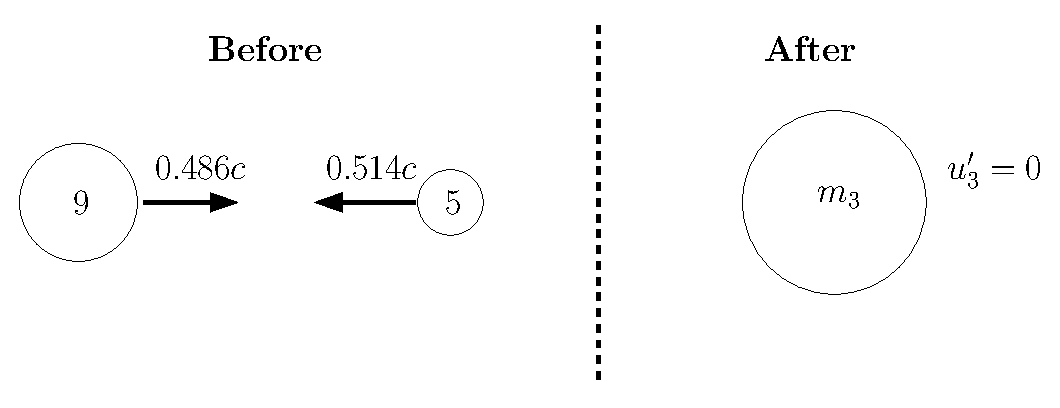
\includegraphics[width=3.8in]{relativistic_momentum_and_energy/relpande2.eps}
\end{center}
\caption{Collision discussed in Example \ref{ex:momentum-goodbye} as
viewed from rest frame of product particle.}
\label{fig:momentum_goodbyeII}
\end{figure}
In the new primed frame, the collision appears as in
Fig.~\ref{fig:momentum_goodbyeII}.  Checking the classical momentum
conservation law in the new frame gives
\begin{equation}
9\units{MeV/$c^2$}\times 0.486c + 5\units{MeV/$c^2$}\times (-0.514c) = 
   m_3 \times 0.
\end{equation}
But the left side of this equation here works out to be
$1.80\units{MeV/$c$}$ which is NOT equal to the right side (which is
0).  So, classical momentum is not conserved in this new frame.
Therefore, either (a) conservation of momentum isn't a valid law of
physics; (b) the Relativity Principle (invariance of the laws of
physics) is violated; or (c) we need a new definition for momentum.
\end{example}

You probably won't be surprised to hear that Einstein wasn't about to
give up on the Relativity Principle because of this argument.  After
all, he had already redefined time and space to make the Principle
work.  And although the classical expression for momentum does not lead to
invariance for high velocity collisions, there are attributes of
particles involving their masses and velocities that do produce
invariant conservation laws.  These quantities are called relativistic
momentum and relativistic energy, or more simply, momentum and energy.
They are defined by

\boxiteq{
\begin{equation}
\vec{p} = \frac{m\vec{u}}{\sqrt{1-u^2/c^2}} 
        \text{\hspace{0.2in}{\bf Definition of relativistic momentum}},
\label{eq:rel-p-def}
\end{equation}}

and

\boxiteq{
\begin{equation}
E = \frac{mc^2}{\sqrt{1-u^2/c^2}} 
\text{\hspace{0.2in}{\bf Definition of relativistic energy}}.
\label{eq:rel-e-def}
\end{equation}}

Einstein was motivated to define momentum and energy in this way
because conservation of momentum and energy defined in this
new way are invariant, as we will show with an example below.  Of
course, motivation is all very nice, but the most compelling reason
that the momentum and energy of a particle must be defined this way
instead of in the classical way is because experiments with high-speed
particles it is these new relativistic quantities that are conserved,
and not those given by the classical definitions.

Let's explore this invariance by redoing Example \ref{ex:momentum-goodbye} 
using Einstein's new definitions and the relativistic conservation laws:
\begin{equation}
\vec{p}_{\rm before} = \vec{p}_{\rm after}
\end{equation}
\begin{equation}
E_{\rm before} = E_{\rm after}
\label{eq:econs}
\end{equation}


\begin{example}{}
\label{ex:pe-cons}
Figure \ref{fig:junk} shows a particle of mass $9\units{MeV/$c^2$}$ and 
speed $0.8c$ striking a stationary particle of mass $5\units{MeV/$c^2$}$, 
producing a single particle of mass $16\units{MeV/$c^2$}$.
You might not be too happy here with the final particle having a mass
of $16\units{MeV/$c^2$}$, but hold on a little longer --- we'll
explain this shortly.  (A little preview --- this might be a good time
to take a pen and scribble Eq.~(\ref{eq:mcons}) out of existence.)  In
the next chapter, we'll learn more rigorously how to determine the
correct attributes of the final particle.  Here we just want to check
the conservation laws. (a) Check the conservation of relativistic
momentum and relativistic energy in the rest frame of the 
$5\units{MeV/$c^2$}$ particle.  (b) Check the conservation of
relativistic momentum and relativistic energy in the rest frame of the
$16\units{MeV/$c^2$}$ particle.
\begin{figure}[tb]
\begin{center}
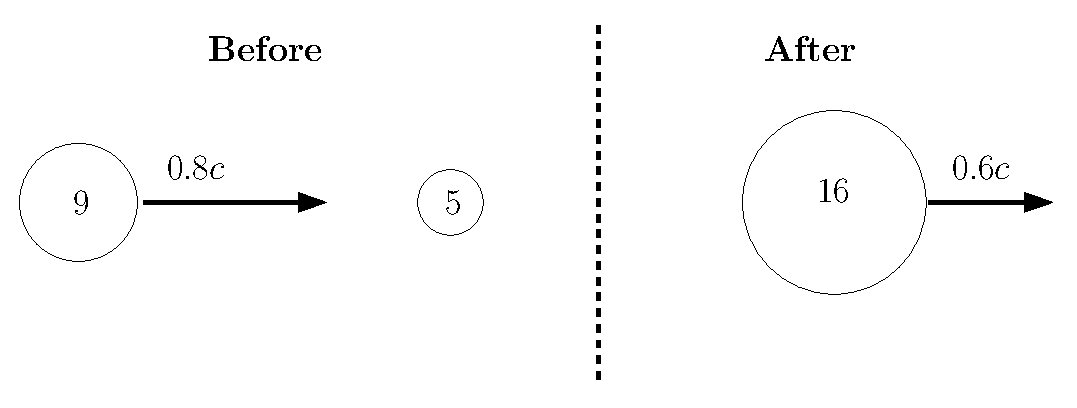
\includegraphics[width=3.8in]{relativistic_momentum_and_energy/relpande3.eps}
\end{center}
\caption{Collision discussed in Example \ref{ex:pe-cons}.}
\label{fig:junk}
\end{figure}

\solution
(a) We will use the relativistic definitions and conservation laws given 
in Eqs.~(\ref{eq:rel-p-def})--(\ref{eq:econs}).  Conservation of momentum 
gives 
\begin{equation}
\frac{9\units{MeV/$c^2$}\times 0.8c}{\sqrt{1 - 0.8^2}} + 0 = 
\frac{16\units{MeV/$c^2$}\times 0.6c}{\sqrt{1 - 0.6^2}},
\end{equation}
and conservation of energy gives
\begin{equation}
\frac{9\units{MeV/$c^2$}\times c^2}{\sqrt{1 - 0.8^2}} 
 + \frac{5\units{MeV/$c^2$}\times c^2}{\sqrt{1 - 0^2}}= 
\frac{16\units{MeV/$c^2$}\times c^2}{\sqrt{1 - 0.6^2}}.
\end{equation}
The momentum equation gives $12\units{MeV/$c$} = 12\units{MeV/$c$}$, 
while the energy equation gives $15\units{MeV} + 5\units{MeV} = 20\units{MeV}$.
So the conservation laws are satisfied in this frame.

(b) Now, transform to a frame in which the final particle is at rest, by
viewing from a spaceship moving at $0.6c$ to the right.  The velocity
transformations give
\begin{eqnarray}
u_{16}^\prime &=& \frac{u_{16}-v}{1 - u_{16}v/c^2} 
   = \frac{0.6c -0.6 c}{1-0.6^2} = 0 \\
u_{5}^\prime &=& \frac{u_{5}-v}{1 - u_{5}v/c^2} 
   = \frac{0 -0.6 c}{1-0\times 0.6} = -0.6c = -\frac{3}{5}c \\
u_{9}^\prime &=& \frac{u_{9}-v}{1 - u_{9}v/c^2} 
   = \frac{0.8c -0.6 c}{1-0.8\times 0.6} = \frac{5}{13}c \simeq 0.385c 
\end{eqnarray}
\begin{figure}[b]
\begin{center}
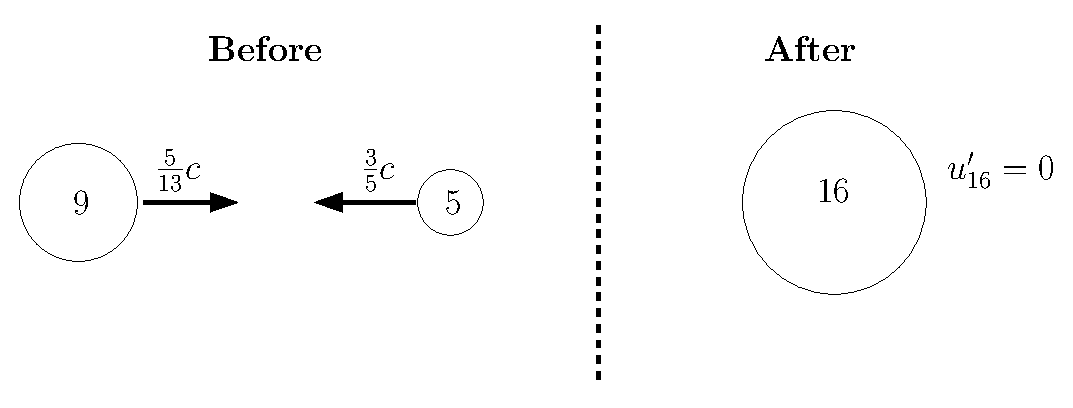
\includegraphics[width=3.8in]{relativistic_momentum_and_energy/relpande4.eps}
\end{center}
\caption{Collision discussed in Example \ref{ex:pe-cons} as viewed from 
rest frame 
of product particle.}
\label{fig:junk2}
\end{figure}
In this new frame, the collision appears as in Fig.~\ref{fig:junk2}.
When we check the relativistic conservation laws in this new frame, we find: 
\begin{equation}
\frac{9\units{MeV/$c^2$}\times 5c/13}{\sqrt{1 - (5/13)^2}} 
    -  \frac{5\units{MeV/$c^2$}\times 3c/5}{\sqrt{1 - (3/5)^2}}= 
\frac{16\units{MeV/$c^2$}\times 0}{\sqrt{1 - 0^2}}
\end{equation}
\begin{equation}
\frac{9\units{MeV/$c^2$}\times c^2}{\sqrt{1 - (5/13)^2}} 
 + \frac{5\units{MeV/$c^2$}\times c^2}{\sqrt{1 - (3/5)^2}}= 
\frac{16\units{MeV/$c^2$}\times c^2}{\sqrt{1 - 0^2}}
\end{equation}
The momentum equation gives
\begin{equation}
\frac{15}{4}\units{MeV/$c$} -\frac{15}{4}\units{MeV/$c$} = 0,
\end{equation}
which checks out, while the energy equation gives
\begin{equation}
\frac{39}{4}\units{MeV} +\frac{25}{4}\units{MeV} = 16\units{MeV}
\end{equation}
which also checks out.  This means the conservation laws are true in
both the original and the new frame, and the Relativity Principle is
upheld with Einstein's new definitions.
\end{example}


This may be a nice argument on paper, but does it work in practice?
Are relativistic momentum and energy, rather than classical momentum
and mass, really conserved in particle interactions?  The answer is an
emphatic {\bf YES}!  In countless interactions observed in high-energy
particle accelerators, relativistic momentum and energy are always
found to be conserved.

\section{Another Invariant}

We now have relativistic expressions for energy and momentum.
It turns out that these can be combined to form an invariant, just
like we combined distance and time to get the invariant spacetime
interval.  Recall from chapter 4, we defined the square of the
interval as
\begin{equation}
I^2 = \left(c\Delta t\right)^2 - \left(\Delta x\right)^2.
\end{equation}
We can combine energy and momentum of an object or particle in a
similar manner to get an invariant:
\begin{equation}
m^2 = \left(\frac{E}{c^2}\right)^2 - \left(\frac{p}{c}\right)^2.
\label{eq:m-invariance1}
\end{equation}
Given any object or particle with energy $E$ and momentum $p$ as
measured by an observer in a reference frame, this observer can easily
calculate the value of $m$ for that object.  If a different observer is
in another reference frame (labeled with ``primes") and determines 
$E^\prime$ and $p^\prime$ for the same particle, she will find that 
if she calculates
\begin{equation}
\left(m^\prime\right)^2 = \left(\frac{E^\prime}{c^2}\right)^2 
          - \left(\frac{p^\prime}{c}\right)^2,
\end{equation}
then she will get exactly the same value for $m^\prime$  that the first
observer found for $m$.  In other words
\begin{equation}
m=m^\prime,
\end{equation}
or
\begin{equation}
E^2 - (pc)^2 = \left(E^\prime\right)^2 - \left(p^\prime c\right)^2.
\label{eq:m-invariance2}
\end{equation}
In the same manner that we used the invariant spacetime interval to
relate $\Delta x$ and $\Delta t$ as measured in one reference frame to 
$\Delta x^\prime$ and $\Delta t^\prime$ in
another reference frame, we can use the invariance of $m$ to relate $E$
and $p$ in one frame to $E^\prime$ and $p^\prime$ in a different frame.

What is this invariant $m$?  This is simply the mass of the object.
In words, the invariance expressed in
Eqs.~(\ref{eq:m-invariance1}--\ref{eq:m-invariance2}) states that
all observers agree about the mass of an object.\footnote{You may hear
people saying that in relativity, ``a person's mass increases as (s)he
approaches the speed of light.''  (In fact, it used to be common for
physicists to say this.)  This is an unfortunate claim.  What they are
doing is saying, ``Well, since $p = mu/\sqrt{1-u^2/c^2}$, we're going
to artificially call $m/\sqrt{1-u^2/c^2}$ the relativistic mass so
that we can hold on to the $p=mu$ definition of momentum.''  There is
no reason to do this --- there is nothing in relativity that requires
us to redefine mass and, in fact, mass is an invariant.}

We can rewrite Eq.~(\ref{eq:m-invariance1}) in a slightly more
convenient form
\begin{equation}
E^2 - (pc)^2 = (mc^2)^2.
\label{eq:m-invariance3}
\end{equation}
As we'll see in the next chapter, this is actually the most useful of
all the energy and momentum relations.  It applies to {\em every}
particle in {\em every} situation.  (We'll see that
Eqs.~(\ref{eq:rel-p-def}) and (\ref{eq:rel-e-def}) aren't very useful
for `particles' of light.)  In the homework for tonight, you'll show
that this relation comes very easily from the relativistic definitions
for energy and momentum (\ref{eq:rel-p-def}) and (\ref{eq:rel-e-def}).


\section{Rest Energy and Kinetic Energy}
Let's look more closely at what we called the relativistic energy of a
particle in Eq.~(\ref{eq:rel-e-def}).  If the particle is at rest, so
that $u = 0$, the energy reduces to $E = mc^2$, perhaps the most famous
formula in all of physics.  So we discover that a particle has energy
even when it's not moving!  This energy is called the {\em rest energy}, 
$E_0$.  That is
\begin{equation}
E_0 = mc^2.
\label{eq:emc2}
\end{equation}
This is a remarkable result! Consider an apple with a mass of 
$100\units{g}=0.1\units{kg}$.    Einstein
says that this apple has an energy at rest of $E_0 = 
0.1\units{kg}\times (3\times 10^8)^2 = 9\times 10^{15}\units{J}$!
This is a huge amount of energy. Let's compare this to a classical 
energy.

You know that the classical kinetic energy of a particle is 
$K_{\rm class.}  = \frac{1}{2}mv^2$.  For the $0.1\units{kg}$ 
apple falling at $10\units{m/s}$ we get $K_{\rm class.} = 5\units{J}$.  
This is the energy that the apple has because it is in motion.
In relativistic physics, kinetic energy is not expressed as 
$K = \frac{1}{2}mv^2$,  but it is still defined as the energy that 
a particle has {\em because it is in motion}.  The relativistic 
kinetic energy is the difference between a particle's energy when 
it is moving and its rest energy, 
\begin{equation}
K = E - mc^2 = \frac{mc^2}{\sqrt{1-u^2/c^2}} - mc^2.
\label{eq:rel-k-def}
\end{equation}
This doesn't resemble the classical expression for kinetic
energy $K_{\rm class.} = \frac{1}{2}mv^2$ (or, since we
use $v$ for the velocity of the frame and $u$ as the velocity of the
particle, $K = \frac{1}{2}mu^2$).  Since we know that the classical
expression for kinetic energy is valid in the low-speed regime, the
relativistic kinetic energy given be Eq.~(\ref{eq:rel-k-def}) must
somehow reduce to the classical expression when the speed of the
particle is small compared to the speed of light.  We show the
connection between the relativistic and classical forms of kinetic
energy in the next example.

The relativistic expressions for energy and kinetic energy have 
amazing consequences.  In collisions of high speed particles, or 
in radioactive decays, it is the total energy of a system of 
particles that is conserved, not the mass.  In these processes,
rest energy ($mc^2$) can be converted into kinetic energy, and vice 
versa.  In a decay, the loss of a small amount of mass corresponds to the 
loss of a huge amount of rest energy, which will be manifested 
in a huge increase in kinetic energy. 
 
 


%However, this doesn't resemble the classical expression for kinetic
%energy, which as you recall was $K = \frac{1}{2}mv^2$ (or, since we
%use $v$ for the velocity of the frame and $u$ as the velocity of the
%particle, $K = \frac{1}{2}mu^2$.).  Since we know that the classical
%expression for kinetic energy is valid in the low speed regime, the
%relativistic kinetic energy given be Eq.~(\ref{eq:rel-k-def}) must
%somehow reduce to the classical expression when the speed of the
%particle is small compared to the speed of light.  We show the
%connection between the relativistic and classical forms of kinetic
%energy in the next example.



% --- the implications are two-fold: first,
%the relation implies that matter and energy aren't separate
%quantities, but are really just different forms of the same thing; and
%second, implied in this relation is the possibility of converting
%between matter and energy.  {\em And the conversion factor is $c^2$
%--- a huge number (when expressed in ``everyday'' units of m$^2$/s$^2$
%or J/kg)!}  To get an idea of the magnitude of this factor, try
%computing the amount of energy contained in a 1 gm paper clip.
%    
%You know from classical physics that the energy associated with a
%particle's motion is called kinetic energy.  However in relativistic
%physics, kinetic energy is not expressed as $K = \frac{1}{2}mv^2$.
%Instead, it is defined as the difference between a particle's energy
%when it is moving and its rest energy,
%\begin{equation}
%K = E - mc^2 = \frac{mc^2}{\sqrt{1-u^2/c^2}} - mc^2.
%\label{eq:rel-k-def}
%\end{equation}
%However, this doesn't resemble the classical expression for kinetic
%energy, which as you recall was $K = \frac{1}{2}mv^2$ (or, since we
%use $v$ for the velocity of the frame and $u$ as the velocity of the
%particle, $K = \frac{1}{2}mu^2$.).  Since we know that the classical
%expression for kinetic energy is valid in the low speed regime, the
%relativistic kinetic energy given be Eq.~(\ref{eq:rel-k-def}) must
%somehow reduce to the classical expression when the speed of the
%particle is small compared to the speed of light.  We show the
%connection between the relativistic and classical forms of kinetic
%energy in the next example.

\begin{example}{Relating relativistic and classical expressions 
for kinetic energy}  

Use the binomial approximation in Eq.~(\ref{eq:rel-k-def}) to find
an approximate expression for $K$ when $u$ is much smaller than
$c$, i.e., when $u/c \ll 1$.  (The binomial expansion states that
$(1-\epsilon)^{-1/2} \simeq 1 + \frac{1}{2}\epsilon + \cdots$ if
$\epsilon$ is small.)

\solution
We write $1/\sqrt{1-u^2/c^2}$ as $(1 - u^2/c^2)^{-1/2}$ so that
Eq.~(\ref{eq:rel-k-def}) becomes
\begin{eqnarray}
K &=& mc^2\left(1-u^2/c^2\right)^{-1/2} - mc^2 \nonumber \\
  &=& mc^2 \left(1 + \frac{1}{2}\frac{u^2}{c^2} + \cdots\right) - mc^2 \\
  &\simeq&  \frac{1}{2}mu^2 \nonumber, 
\end{eqnarray}
where in the last line we have assumed the classical limit in which
$u/c \ll 1$.
Thus we see that the classical expression for kinetic energy is only a
low-velocity approximation to the correct expression, given by
Eq.~(\ref{eq:rel-k-def}).
\end{example}

\section{Photons: Particles with Zero Mass}

How do we deal with the energy and momentum of light? As you will see
next semester in PHYS 212, the same year that Einstein published his
first paper on Special Relativity, he also proposed that light must be
considered to be composed of particles which are now called photons.
(This was the first of the three 1905 papers that we discussed at the
beginning of Chapter \ref{chapter:relativityI}.)  Since light always travels
at a speed $c$ in a vacuum, then photons in a vacuum must travel at
that speed regardless of the reference frame of the observer.  But if
we look back at Eqs.~(\ref{eq:rel-p-def}) and (\ref{eq:rel-e-def}), we
find that the denominators of both equations are zero for a particle
moving at the speed of light, and clearly a photon cannot have
infinite momentum or infinite energy.

    
The only way to resolve this dilemma is to postulate that photons are
particles with zero mass ($m = 0$).  Equations~(\ref{eq:rel-p-def})
and (\ref{eq:rel-e-def}) are still not very useful in this case, since a
fraction which has zero in both the numerator and denominator is
undefined.  However, with zero mass these equations no longer imply 
infinite energy and momentum for particles moving at light speed.
    
For a massless particle (such as photons),
Eq.~(\ref{eq:m-invariance3}) can be rewritten for $m=0$ as
\begin{equation}
E = \vert p\vert c\text{\hspace{0.25in}{\bf for massless particles only.}}
\label{eq:e-photon}
\end{equation}
Remember, Eq.~(\ref{eq:e-photon}) is valid only for massless
particles.

\section{More experimental evidence}

Now that we have introduced the relativistic relations for energy and
momentum, we can discuss some additional pieces of evidence that
Einstein's theory of relativity is, in fact, correct.  The following
examples can be added to those presented in Chapter
\ref{chapter:relativityI}.  Remember that if even one of these
experiments had disagreed with Einstein's theory, then the entire
theory would have to be thrown out since everything is internally
consistent.
\begin{itemize}
\item {\bf Particle accelerators}. As we already discussed in
Chapter~\ref{chapter:relativityI}, subatomic particles are frequently
accelerated in high energy experiments to speeds very close to $c$,
but no one has ever managed to accelerate a particle with mass to a
speed greater than $c$.  There's more here, though: as the particle's
speed (relative to the laboratory) gets closer and closer to $c$, the
amount of energy that has to be added to increase the speed further
gets larger and larger, diverging as the speed approach $c$.  For
instance, the amount of energy that needs to be added to accelerate a
particle from $0.98c$ to $0.99c$ has been found experimentally to be much
larger than the energy to accelerate the same particle from $0.97c$ to
$0.98c$, and in fact, much larger than that predicted classically.  As
is the case with all other tests of relativity, the amount of energy
to be added agrees perfectly with Einstein's predictions.  Homework
problem \ref{prob:energy-to-accelerate}  investigates this further.
\item {\bf Collisions of high-energy particles}.  When subatomic
particles are slammed into each other with high energies, new
particles are actually created that weren't there before the
collision.  These collisions are converting kinetic energy (KE) into
matter, and this is done all the time in particle accelerators.  (This
is, in fact, the main tool that physicists use to study massive
subatomic particles.)  This is an experimental result that simply
cannot be explained classically.  Once again, though, the results
agree perfectly with Einstein's theory.  We will be discussing this in
more detail in Chapter \ref{chapter:relativity_app}, and you will be doing
(or have already done) a lab on this (the Relativistic Energy and
Momentum lab).
\item {\bf Matter-to-KE conversions}.  One of the most convincing and
most dramatic tests of Einstein's theory of relativity occurred on
July 16, 1945, in New Mexico when the first atomic bomb was exploded,
converting matter into a horrifying amount of kinetic energy (don't
forget that factor of $c^2$ in the famous $E = mc^2$ equation).  Since
then, there have been quite a few additional such demonstrations of
Einstein's theory.  (And again, the quantitative aspects of these
demonstrations agree perfectly with the theory.)
    
It isn't necessary to explode a bomb to convert matter into energy.
Nuclear energy has found peaceful applications in the area of power
generation. (There is a nuclear power plant in Berwick, PA, in fact,
which you can see easily if you drive on Rt.~80 toward New Jersey,
shortly after passing Bloomsburg).  We will discuss nuclear power
generation more in the next chapter (including fusion power ---  still
being developed --- which doesn't produce any long-lasting radioactive
waste).

\end{itemize}

\section{A note on units}
\label{section:rel-units}

When working with energy and momentum for small, subatomic particles
(the ones that are most typically traveling at relativistic speeds),
it is convenient to define a unit of energy called the ``electron
volt'' (eV for short).  One electron volt is the kinetic energy gained
by an electron when accelerated through a 1 volt potential difference.
(You'll learn more about this in PHYS 212.)  Quantitatively, $1\units{eV} =
1.6\times 10^{-19}\units{J}$.  An analogous energy unit might be a
``superball-meter'' --- the amount of kinetic energy gained by a
superball when dropped 1 m.
    
For high energy particles, the energies can get into the thousands,
millions or billions of electron volts, so we also define 
$1\units{keV} = 10^3\units{eV}$, $1\units{MeV} = 10^6\units{eV}$,
$1\units{GeV} = 10^9\units{eV}$.
    
Units for mass and momentum are also defined in terms of energy in
relativity.  For mass, we use eV/$c^2$ --- ``electron volts per
$c^2$'' --- or keV/$c^2$, MeV/$c^2$, GeV/$c^2$.  For momentum, we use
eV/$c$ (or keV/$c$, MeV/$c$, GeV/$c$).  For example, an electron has a
mass of $511\units{keV/$c^2$}$; conceptually, this means that an electron 
has a rest energy of $511\units{keV}$, or that its mass --- if converted 
completely into kinetic energy --- would produce $511\units{keV}$ of 
kinetic energy.
  
{\bf Warning}: when using these units, don't throw any numbers in for
the $c$ --- it is part of the unit.  So, the mass of an electron
should be written as ``$511\units{keV/$c^2$}$'' (or $0.511\units{MeV/$c^2$}$), 
{\bf not} as $511\units{keV}/(3.0\times 10^8\units{m/s})^2$ \hspace{-1.7in}\rule[1mm]{42mm}{.2mm} 
or $511\units{keV}/(1\units{lt-s/s})^2$.\hspace{-1.25in}\rule[1mm]{30mm}{.2mm}
\newpage

\section{Summary}
The various equations introduced in this chapter are summarized as
in Table \ref{table:rel-defs}.

\begin{table}[h]
\begin{small}
\caption{Relativistic formulas for energy and momentum.}
\label{table:rel-defs}
\begin{tabular}{|lclc|} \hline
\parbox{3.0cm}{\raggedright{\bf Definition of momentum:}}   &  
       \parbox{3.cm}{\[ \vec p =\frac{m\vec u}{\sqrt{1-u^2/c^2}} \]} & 
\parbox{3.0cm}{\raggedright{\bf Definition of energy:}} & 
       \parbox{3.cm}{\[ E =\frac{mc^2}{\sqrt{1-u^2/c^2}} \]} \\
\parbox{3.0cm}{\raggedright {\bf Energy in terms of momentum and mass:}}   &  
       \parbox{3.cm}{\[ E^2 = p^2c^2 + m^2c^4\]} & 
\parbox{3.0cm}{\raggedright{\bf Velocity in terms of energy and momentum:}\\
       (See Problem \arabic{chapter}.\ref{prob:rel-u-p-e}.)} & 
       \parbox{3.cm}{\[ \vec{u} = \frac{\vec{p}c^2}{E} \]} \\
       & & & \\
\parbox{3.0cm}{\raggedright{\bf Definition of kinetic energy:}}   &  
       \parbox{3.cm}{\[ K = E - mc^2 \]} & 
\parbox{3.0cm}{\raggedright{\bf Energy in terms of momentum for 
zero-mass particle:}} & 
       \parbox{3.cm}{\[ E = \left|\vec{p}\right|c \]} \\
&  & & \\ \hline
\end{tabular}
\end{small}
\end{table}

\newpage

\section*{Problems}
\markright{PROBLEMS}

\begin{problem}
Duck Dodgers hops in his spaceship and leaves the Earth at a
speed $0.6c$ in an attempt to reach the newly discovered Planet X before
aliens from Mars.
    \begin{enumerate}
    \item Mission control on Earth sends an encoded message (a
    flashing beacon) to Duck Dodgers warning him about the progress of
    the Martian ship.  The light pulses travel at a speed $c$ relative
    to observers on the Earth.  How fast are the pulses traveling
    relative to Duck Dodgers?
    \item Duck Dodgers doesn't understand the message that he
    received, so he sends a radio message back toward the Earth asking
    for clarification.  The radio signal is traveling at a speed $c$
    relative to the Duck.  How fast is the signal traveling relative
    to observers on the Earth?
    \item The radio message is intercepted by the Martian who is
    behind Duck Dodgers but traveling in the same direction at a speed
    $0.8c$ relative to the Earth.  How fast is the radio message going
    relative to the Martian?
    \item The radio message is also intercepted by one of the
    Martian's monsters who is traveling back toward the Earth to
    attack.  The monster is traveling at a speed $0.9c$ relative to the
    Martian.  How fast is the radio signal relative to the monster?
    \end{enumerate}
\end{problem}

\begin{problem}
A particle travels at speed $0.50c$ relative to Captain Kirk.
Mr.\ Spock is traveling at a speed $0.70c$ relative to Captain Kirk,
in the same direction as the particle.
Calculate the velocity of the particle relative to Mr.\ Spock.
\label{prob:vtransform}
\end{problem}

\begin{problem}
A proton's velocity is measured at $0.6c$ relative to an observer
on earth, and $0.8c$ relative to an observer passing by in a rocket.
Determine the speed of the rocket relative to earth.  (There 
are two possible correct answers that correspond to two different
physical situations.)
\label{prob:vtransform2}
\end{problem}

\begin{problem}
After traveling on vacation to Betelgeuse to witness a supernova, Fred
and Ethel are returning home, traveling at a speed $0.75c$ relative to
and toward the Earth.  Ethel is particularly anxious to get home and
see her new great-great-great-great-great-great-great-great grandson,
so she hops on the emergency shuttlecraft, which leaves Fred's ship
traveling at a speed of $0.75c$, relative to Fred.  How fast is Ethel's
shuttle traveling relative to the Earth?
\end{problem}

\newpage
\begin{problem}
A particle of mass $3m$, moving at speed $0.60c$ in the positive
$x$-direction, collides with and sticks to a particle of mass $2m$
originally at rest.  Assume a head-on collision.
\begin{enumerate}
\item Calculate the initial total momentum before impact, using the
classical definition, $p = mu$, for momentum. 
\item Assuming conservation of mass as well as classical momentum,
find the velocity of the composite particle of mass $5m$ after the
collision.  
\item Now transform to a primed frame in which the particle of mass
$3m$ is at rest.  Use the relativistic velocity transformation to
compute the velocities $u^\prime_{3m}$, $u^\prime_{2m}$, and
$u^\prime_{5m}$ in the primed frame. 
\item Still in the primed frame, check whether momentum $mu^\prime$ is
conserved by computing the total momentum before the collision and the
total momentum after the collision.
\end{enumerate}
\label{prob:inelastic}
\end{problem}


\begin{problem}
Show that the velocity of a particle expressed in terms of
relativistic energy and momentum is $u = pc^2/E$.
\label{prob:rel-u-p-e}
\end{problem}


\begin{problem}
An electron is accelerated from a velocity $u_1 = 0.98c$ to a velocity
$u_2 = 0.99c$.  Calculate the change in the electron's kinetic energy in
units of MeV.  ($m_{\rm electron} = 0.511\units{MeV/$c^2$}$.)
\label{prob:energy-to-accelerate}
\end{problem}

\begin{problem}
Electron A has a total energy of $1.0\units{MeV}$.  Electron B has a
kinetic energy of $0.25\units{MeV}$.  Electron C has a kinetic energy of
$0.75\units{MeV}$.  Electron D has a momentum of $1.0\units{MeV/$c$}$.
For each of the electrons A through D, determine its energy, momentum,
kinetic energy, and speed.
\label{prob:electrons}
\end{problem}

\begin{problem}
A certain particle has a total energy of $1.20\units{MeV}$ and
a momentum of $0.95\units{MeV/$c$}$.  Calculate the particle's mass,
kinetic energy, and velocity.  
\end{problem}

\begin{problem}
Compute the momentum and velocity of a proton that has a total
energy equal to 7 times its rest energy.  ($m_{\rm proton} =
938\units{MeV/$c^2$}$.)
\label{prob:proton}
\end{problem}

\begin{problem}
Combine Eqs.~(\ref{eq:rel-p-def}) and (\ref{eq:rel-e-def}) to derive 
Eq.~(\ref{eq:m-invariance3}).
\end{problem}

\begin{problem}
Show, from Eq.~(\ref{eq:m-invariance3}) and the result of
problem (\ref{prob:rel-u-p-e}) that any massless particle moves at
the speed of light and that if a particle moves at the speed of light
it must have zero mass.    
\end{problem}

\begin{problem}
A proton (mass $938\units{MeV/$c^2$}$) is traveling at velocity
$0.60c$ in the $+x$ direction relative to a spaceship which itself is
traveling at velocity $0.80c$ in the $+x$ direction relative to Earth.
Calculate the velocity and then the energy and momentum of the proton
as measured in the Earth frame.
\end{problem}

\begin{problem}
A particle's energy and momentum in one frame are $41\units{MeV}$ and 
$40\units{MeV/$c$}$ respectively.  Find the particle's energy and 
momentum as measured in a different frame in which the particle's speed is 
$u^\prime = 0.8c$.
\label{prob:ep_transform}    
\end{problem}

\begin{problem}
Given a particle with $E_A = 21\units{MeV}$ and $p_A
= 15\units{MeV/$c$}$ as measured in reference frame {\bf A}, and 
$E_B = 20\units{MeV}$ as measured in frame {\bf B}, determine the 
mass $m_B$ and momentum $p_B$ of the particle as measured in 
frame {\bf B}.  
\end{problem}

\begin{problem}
The Fermi National Accelerator Laboratory (Fermilab) is located outside
Chicago, Illinois, and is one of the world's largest particle accelerator
facilities.  At Fermilab, protons (mass $938\units{MeV/$c^2$}$) are given
huge amounts of energy and achieve velocities that are nearly the speed
of light.
\begin{enumerate}
\item Prior to a recent upgrade, protons at Fermilab could reach
speeds that were only $163\units{m/s}$ slower than the speed of
light.  How much energy is required to get a proton from rest up to
the speed $u = c - 163\units{m/s}$?  
\item After the upgrade, the protons were able to reach the speed $u
=c - 132\units{m/s}$ (a whopping increase of $31\units{m/s}$).
How much additional energy is required to get this $31\units{m/s}$
increase?
\item The Large Hadron Collider currently being developed at CERN (a
  particle accelerator facility in Europe) is designed to get protons
  up to an energy of $7.0\units{TeV}$. ($1\units{TeV} =
  10^{12}\units{eV}$).  Determine $u/c$, the ratio of the speed of the
  proton to the speed of light (note that $u/c$ is NOT equal to 1!)
\end{enumerate}
\label{prob:fermilab}
\end{problem}

\begin{problem}
A certain J-boson has mass of $150\units{MeV/$c^2$}$, speed of
$0.8c$, and total energy of $250\units{MeV}$.  Determine
the J-boson's momentum and kinetic energy.
\label{prob:J}
\end{problem}

\begin{problem}
A proton (mass $938\units{MeV/$c^2$}$) traveling down a beam pipe at
Fermilab is determined to have kinetic energy of $1.2\units{GeV}$.
Determine this proton's momentum and speed.
\label{prob:fermilab2}
\end{problem}
\newpage

\begin{problem}
An evil genius fires a rocket into a star, destroying the star.
Ten minutes later, as measured in the reference frame of the star,
debris thrown out from the explosion demolishes a
populated planet a distance $7\units{lt-min}$ from the star, as measured
in the star/planet frame.  Simultaneous with the explosion (according
to the star/planet reference frame), the Starship
Enterprise is $5\units{lt-min}$  from the star, on the opposite side from
the planet.  The Enterprise is
heading toward the star/planet system with a
speed of $0.6c$ relative to the planet and star.
\begin{enumerate}
     \item Draw a spacetime diagram for this situation.  Take the
       star/planet reference frame as the unprimed frame, and draw the
       world lines of the star and the planet, showing that they are
       $7\units{lt-min}$ apart.  Indicate the destruction of the star
       as event A on your spacetime diagram, and indicate the
       destruction of the planet as event B on your spacetime diagram.
       Also, draw the world line for the debris sent from the star to the
       planet.
     \item Draw the world line of the Starship Enterprise on your spacetime
     diagram, showing both the velocity of the spaceship and the correct
     location of the Enterprise when the star explodes.
    \item Calculate the speed of the matter thrown out from the explosion
     as measured by Starfleet officers on board the Enterprise.
     \item Calculate the time interval between the explosion of the star
     and the destruction of the planet, as measured by Starfleet officers
     on board the Enterprise.  (Hint:  use your result from (c) to
     determine an expression for the distance between events ---
     according to the Enterprise --- in terms of the unknown time between
     events.)
     \end{enumerate}
\label{prob:evil_genius}
\end{problem}
\newpage

\begin{problem}{\bf Are momentum and energy conserved?}\\
A mad scientist at rest in a lab on the earth is colliding particles together
to make more massive particles.  She creates head-on collisions of 
particles with a mass of $4\units{GeV/$c^2$}$ and speed $0.6c$ to create 
particles at rest with a mass of $10\units{GeV/$c^2$}$.

In the rest frame of the scientist, the  $4\units{GeV/$c^2$}$ particles
have equal and oppositely directed momenta, and the $10\units{GeV/$c^2$}$
particle is at rest, so momentum is conserved.

An observer in a rocket flying over the lab at a speed $v=0.6c$ views this 
experiment.  

\begin{enumerate}
\item Test whether {\bf relativistic} momentum is conserved 
according to the observer in the rocket.  Your test should include 
detailed numerical calculations  demonstrating the conservation 
(or non-conservation) of {\bf relativistic} momentum.
\item  Test whether {\bf relativistic} energy is conserved 
according to the scientist in her lab.  Your test should include 
detailed numerical calculations demonstrating the conservation 
(or non-conservation) of {\bf relativistic} energy.
\item  Test whether {\bf relativistic} energy is conserved 
according to the observer in the rocket.  Your test should include 
detailed numerical calculations demonstrating the conservation 
(or non-conservation) of {\bf relativistic} energy.
\end{enumerate}
 
 \begin{figure}[h]
    \begin{center}
    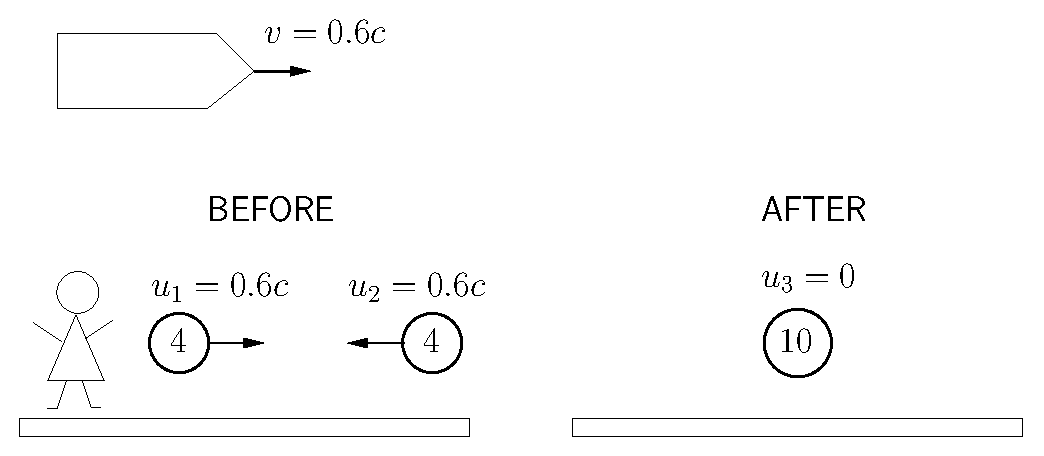
\includegraphics[width=4.25in]{relativistic_momentum_and_energy/atomsmasher.eps}
    \end{center}
    \caption{Figure for Problem \ref{prob:is_momentum_conserved}.}  
    \label{fig:is_momentum_conserved}
  \end{figure}

\label{prob:is_momentum_conserved}
\end{problem}


%\chapter[Applications of the Conservation Laws]{Applications of the 
Relativistic Conservation Laws}
\label{chapter:relativity_app}

%\section*{Objectives}
%\begin{objectives}
%\item Describe increases and decreases in mass associated with processes
%that release or absorb kinetic energy.
%\item Apply the relativistic conservation laws to ``explosions,'' in
%which one particle decays into two particles, including cases in
%which one or both outgoing particles have zero rest mass.  
%\item Do the same for simple collisions with all particles traveling
%along a line.
%\item Be able to describe the processes of nuclear fusion and fission,
%and explain how these processes result in kinetic energy production.  
%\item Given information about nuclear masses, calculate the amount of
%kinetic energy gained in a fusion or fission process.
%\end{objectives}

\section{Introduction}

You should now understand why Einstein's postulates
require new definitions of momentum and energy.  The classical
momentum is not conserved, nor in general is the total mass of the
particles in an interaction.  In place of these, relativistic momentum
and relativistic energy are conserved, and they are conserved in any
inertial frame.  

In this chapter, we apply these new, relativistic conservation laws to 
analyze collisions and decays of subatomic
particles.  The key result in these applications is the ability for
matter to be converted into kinetic energy and vice-versa.  In relativistic
collisions, the amount of matter that you start with is not the same
as the amount of matter that you finish with!  We also discuss the
principles behind nuclear fission and nuclear fusion.

\section{Changes of Rest Energy}
  Much of the light you see comes from changes in rest energy of
atoms.  Examples are sunlight, light from a candle flame, a lightning
flash, light emitted by a fluorescent lamp, light from the phosphor
coating on the screen of a television set or a video monitor, and
laser light.  In all these examples, the basic mechanism is that an
atom in an ``excited'' state releases its energy in the form of a
photon, with the atom going into its ground (lowest possible) state,
or into an excited state of lower energy.  We can represent the
emission process by the simple reaction equation

\begin{equation}
{\bf A}^\ast \rightarrow {\bf A} + \gamma. 
\label{eq:photon_emission}
\end{equation}
Here ${\bf A}^\ast$ represents the excited atom, ${\bf A}$ the atom in its
ground or lowest state, and $\gamma$ (Greek {\em gamma}) the photon.

\begin{figure}[tbp]
\begin{center}
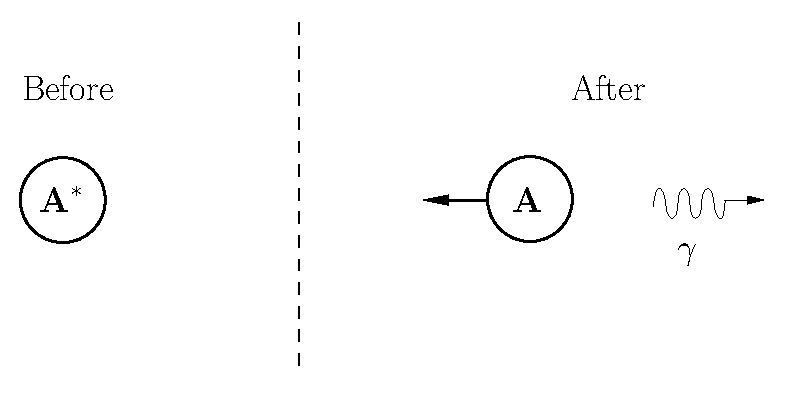
\includegraphics[width=3.5in]{relativity_conservation/photon_emission1.eps}
\end{center}
\caption{An excited atom emits a photon and recoils.}
\label{fig:photon_emission1}
\end{figure}

In Fig.~\ref{fig:photon_emission1}, the excited atom is shown at rest,
so all of its energy is rest energy and it has no momentum.  But the
photon has energy, and from the relation $E = pc$, it also has
momentum.  And because momentum must be conserved, the atom recoils.
We can write the conservation of energy equation for the reaction in
Eq.~(\ref{eq:photon_emission}) as follows
\begin{equation}
\text{Rest Energy of ${\bf A}^\ast$} = \text{Energy of ${\bf A}$} 
+ \text{Energy of photon}.
\end{equation}
     
Because both the kinetic energy of ${\bf A}$ and the photon energy are
positive numbers, the rest energy (i.e., the mass) of the
excited-state atom must be greater than that of the ground-state atom.
Therefore, in the emission process rest energy, i.e., mass, is
converted to kinetic energy.
     
When light is absorbed by an atom, exactly the opposite effect occurs.
The atom begins in its ground state, absorbs the photon energy and
goes into an excited state.  Again, by conservation of energy, the
excited atom must have more rest energy than the ground-state atom.

Another everyday example of changing rest energy occurs in chemical
reactions.  For example, the reaction for the oxidation of a carbon
atom
\begin{equation}
\text{C} + \text{O}_2 \rightarrow \text{CO}_2
\end{equation}
is known to release energy in the form of one or more photons.
Therefore the sum of the masses of C and O$_2$ must be greater than
the mass of the carbon dioxide molecule.  The change in rest energy in
the case of chemical reactions is typically on the order of
$1\units{eV}$ (or $1.6\times 10^{-19}\units{J}$).  Much larger
energies, on the order of $1\units{MeV}$, are involved in nuclear
reactions.  An example of a nuclear reaction is the decay of a neutron
into a proton, an electron, and an electron antineutrino:
\begin{equation}
n \rightarrow p + e^- + \bar{\nu}_e.
\end{equation}
Here the excess mass of the neutron over the mass of the proton plus
electron (the electron antineutrino has very small mass) is converted
to the kinetic energy of the three reaction products.

Another important example of changes in rest mass is the production of
new particles in a high energy particle accelerators.  In these
accelerators high-speed particles are shot at target particles and
some of the kinetic energy of the incoming particles is converted to
rest energy.  In this way hundreds of new particles, most with
lifetimes between $10^{-10}$ and $10^{-23}\units{s}$, have been
produced.  You'll learn more about these new particles next semester
in PHYS 212.

\section[General Strategy]{General Strategy for 
Applying the Relativistic Conservation Laws}


 In a typical problem you are given information about the particles
before an interaction and asked to compute certain properties of the
outgoing particles after the interaction.  You do this by writing down
equations that express the fact that the sum of the incoming momenta
is equal to the sum of the outgoing momenta and the sum of the
incoming energies is equal to the sum of the outgoing energies.  What
quantities should be used in writing these equations?  Here is some
time-saving advice.
\begin{quote}
Always write the conservation of momentum and conservation of energy
equations in terms of momentum and energy or mass variables, never in
terms of velocity or kinetic energy.
\end{quote}

This rule keeps the algebra as simple as possible --- it gets around
having to solve simultaneous equations with the $\sqrt{1-v^2/c^2}$
terms that can make the algebra messy.  For example, if you are given
the velocity of one or more particles in the problem statement, first
calculate the momentum and energy of each particle from the given
velocities.

A second piece of advice:
\begin{quote}
When working with ``eV'' units (e.g., MeV for energy, MeV/$c$ for
momentum, MeV/$c^2$ for mass), don't ever put any numbers in for the
speed of light $c$.  Just leave it as ~``$c$.''  The units will then
automatically take care of themselves.
\end{quote}

For example, if you have an motionless electron, its energy can be
obtained from $E^2 = p^2c^2+m^2c^4$. For a motionless electron  $p = 0$, 
so $E= mc^2 = 0.511\units{MeV/$c^2$}\times c^2 = 0.511\units{MeV}$.  
(See section \ref{section:rel-units}.)

\begin{example}{Emission of a photon by a nucleus.}
\label{ex:nuclear_decay}
An excited atomic
nucleus, of mass $5.00\units{GeV/$c^2$}$ and at rest, as in
Fig.~\ref{fig:photon_emission2}, decays to its ground state by
emitting a photon of energy $2.00\units{GeV}$.  Calculate the recoil
velocity and mass of the ground-state nucleus.
\solution
First draw a picture, and label each particle with its value of
energy and momentum.  Before the decay the excited nucleus has zero
momentum because it is at rest.  And from $E^2 = p^2c^2 + m^2c^4$, with 
$p =0$, we know its energy is the same as its rest energy, namely 
$5.00\units{GeV}$.

\begin{figure}[tbp]
\begin{center}
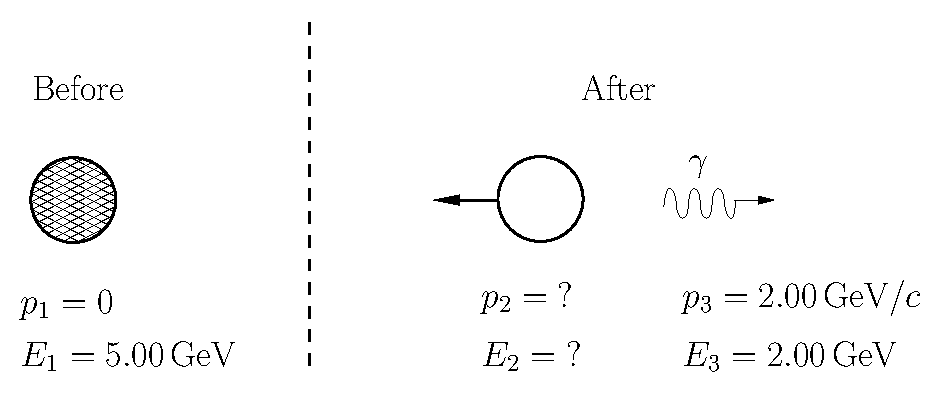
\includegraphics[width=4in]{relativity_conservation/photon_emission2.eps}
\end{center}
\caption{Emission of a photon by a nucleus as discussed in Example 
\ref{ex:nuclear_decay}.}
\label{fig:photon_emission2}
\end{figure}

After the decay the ground-state nucleus recoils with unknown energy
and momentum, $E_2$ and $p_2$.  Also, the emitted photon has an energy
of $2.00\units{GeV}$, as specified in the problem.  And because the
photon's mass is zero its momentum has the same numerical value as its
energy.  Notice that in the diagram there are two unknowns, the
energy and momentum of the recoiling ground-state nucleus.  We plan to
solve for these two unknowns with two equations, the energy and
momentum conservation equations.
     
Looking at the diagram, we write down the energy conservation equation
in terms of the symbols and numerical quantities shown in the
diagram:
\[ 5.00\units{GeV} = E_2 + 2.00\units{GeV}. \]
Similarly, we write the momentum conservation equation in terms of
symbols and numerical quantities shown in the diagram:
\[ 0 = p_2 + 2.00\units{GeV/$c$}.  \] From these conservation-law
equations we easily solve for the energy and momentum of the recoiling
nucleus to obtain $E_2 = 3.00\units{GeV}$ and $p_2 =
-2.00\units{GeV/$c$}$.  Now that we've obtained expressions for the
energy and momentum of the recoiling ground-state nucleus, we can find
its velocity using a formula from Problem
\ref{chapter:relativity_pande}.\ref{prob:rel-u-p-e} (and from Table
\ref{table:rel-defs}):
\[ u_2 = \frac{p_2c^2}{E_2} = \frac{(-2.00\units{GeV/$c$})\times c^2}
           {3.00\units{GeV}} = -\frac{2}{3}, \]
and its mass from 
\begin{eqnarray}
m_2c^2 &=& \sqrt{E_2^2 - p_2c^2} \nonumber \\
       &=& \sqrt{(3.00\units{GeV})^2 - (2.00\units{GeV/$c$})^2 \times
            c^2} \nonumber \\
       &=& \sqrt{5}\units{GeV}, \nonumber 
\end{eqnarray}
so the mass is $m_2 = \sqrt{5}\units{GeV/$c^2$}\simeq 2.24\units{GeV/$c^2$}$.

Notice that even though we were asked to find the velocity and mass
of the recoiling nucleus, we didn't use these variables in our
analysis until the very end, after we solved for its energy and
momentum.
\end{example}

\section[Fusion and fission]{Nuclear masses, fusion and fission}


A particularly important application of the material in this chapter
is nuclear power generation.  There are two main approaches: fusion
and fission.  Nuclear fusion involves the merging (fusing) of two
light nuclei (usually hydrogen) to form a more massive nucleus
(usually helium), whereas fission\footnote{The story of how fission was
discovered is quite interesting. It starts with Lise Meitner and Otto
Hahn, who conducted ``transuranium'' experiments where they bombared 
massive nucleii with the goal of making {\bf more} massive nucleii
(more massive than uranium). But the experiments produced puzzling results.
Meitner -- with her nephew Otto Frisch -- later provided an explanation.
Instead of making more massive nucleii, they realized that the nucleii
were breaking up with a resulting loss of mass, and Meitner used 
Einstein's theory of relativity
to explain the increase in energy observed in the process. Meitner -- who
was inexplicably overlooked for the Nobel Prize for the fission discovery --
also discovered a radiation process which was named the {\em Auger effect}
after a scientist who also discovered this process, a couple of years
{\bf after} Meitner had discovered it.}
 involves the splitting of a very
massive nucleus (e.g., uranium) into two or more lighter nuclei.
For the process to release kinetic energy, conservation of
relativistic energy requires that the end product(s) have a smaller
total mass than the initial nucleus or nuclei.

\begin{figure}[tbp]
\begin{center}
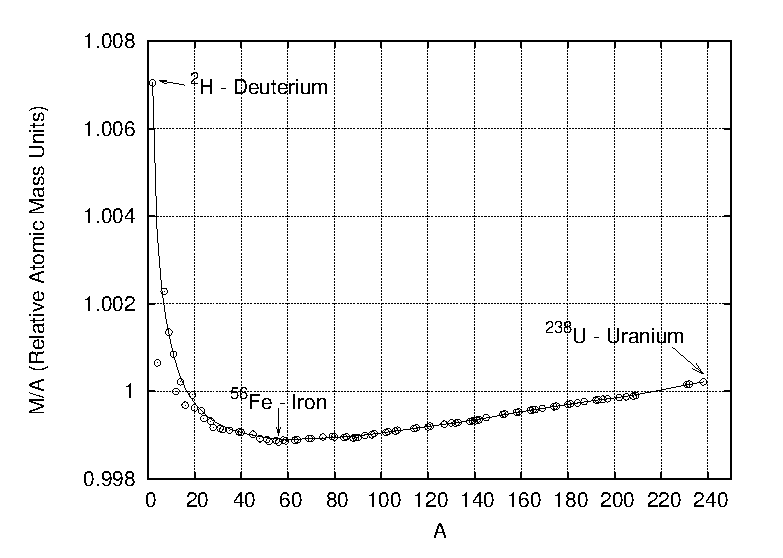
\includegraphics[width=4.5in]{relativity_conservation/mass_per_nucleon.eps}
\end{center}
\caption{Plot of mass per nucleon (proton and neutrons) for the 
elements versus the number of nucleons $A$. (Data from NIST:
http://physics.nist.gov/PhysRefData/Compositions/)}
\label{fig:mass_per_nucleon}
\end{figure}

Figure \ref{fig:mass_per_nucleon} shows a plot of the masses of the
elements, divided by the total number of protons and neutrons
(nucleons) in the nucleus of each atom.  This plot is very
illuminating when considering fusion and fission processes.  
The
fusion of two $^2$H nuclei to form a single $^4$He nucleus results in
a lower overall mass, since the number of nucleons does not change; 
consequently, this process releases kinetic
energy.  On the other hand, elements with large atomic number $A$
have a larger mass/nucleon than those with intermediate values of $A$;
consequently, kinetic energy can also be released by splitting up one of
these heavier atoms (fission).

Of the two processes --- fission and fusion --- fission is a much
easier process to achieve in the laboratory or in industrial
processes.  Many large nuclei are naturally unstable, e.g., $^{235}$U can
spontaneously decay via the fission process ${}^{235}\text{U} \rightarrow
{}^{134}\text{Xe} + {}^{100}\text{Sr} + {}^1n$.  Practically, then, the
issue boils down to setting things up such that the process can be
accelerated when desired, and can be inhibited when unwanted.  From
that perspective, the concept of a chain reaction is relevant.  The
idea of combining multiple nuclear fissions into chain reactions ---which was pioneered
by Lise Meitner, Otto Hahn, Fritz Strassmann, and Enrico Fermi in the
1930s --- is straightforward: if the neutrons that are released in a
fission process bombard another nearby (unstable) nucleus, they can
trigger the fission of that nucleus as well.  Practically, all that is
needed is a large enough density of the unstable nucleus (e.g., $^{235}$U)
 and a chain
reaction will start.  This idea was pursued by the Manhattan Project
in the 1940s to develop an atomic bomb, the detonation of which was
achieved by explosively compressing a uranium sample to increase its
density above the critical value for a chain reaction.  Alternatively,
the strength of the fission chain reaction 
can be controlled by absorbing some of the neutrons
produced in the fission reaction. Graphite  rods
(which absorb neutrons) are commonly used to ``moderate''
the reaction in this way to allow the reaction to proceed in a
controlled manner in power generators.

Nuclear fission power has a few serious drawbacks: (a) the fuel (uranium,
plutonium, etc.) is
expensive and limited in supply.  If society were to switch entirely
to uranium-fission-based power generation, it is estimated that the supply
of uranium would last for only 50-100 years.  (b) The by-products of
the fission reaction are nuclei which themselves are unstable and
radioactive; consequently, the material poses a health hazard unless
properly stored.  (Note: some countries use  techniques to
extract additional energy from this nuclear ``waste.'')
     
Another drawback of nuclear fission reactors --- which is diminishing with
improved technology --- is the concern that they could ``melt down''
and release massive amounts of radiation (this actually happened to
the Chernobyl 4 reactor in the Soviet Union in 1986).  This threat has been
lessened recently by the development of much better systems, including
a ``melt-proof'' system with an expandable core; if the temperature of
the core exceeds a defined value, the core expands, dropping the
density of the fissile material down below its critical value and
stopping the chain reaction.  (This works even if all cooling is
stopped.)  But even this system isn't perfect, as there is always the
concern that a terrorist attack or gross human error could result in
the release of disastrous amounts of radioactive waste into the
environment.

In contrast to fission reactors,  nuclear fusion reactors use water as
their  fuel  (actually the  $^2$H  isotope  of  hydrogen, also  called
deuterium,  which is  found in  small  amounts in  water) and  produce
helium   as  a   by-product,  so   waste   disposal  is   less  of   a
problem.\footnote{Some radioactive tritium  is released in the process
  as well, but it is short-lived  with a half-life of only 12 minutes;
  consequently  there   is  no   long-term  waste  problem   with  the
  tritium. The only long-term waste would be the activated material in
  the reactor  containment vessel  itself.}  The nuclear energy  production is
also much more efficient for this  process than for fission, as can be
inferred     from     the     steepness     of    the     curve     in
Fig. \ref{fig:mass_per_nucleon}.  It is estimated that there is enough
$^2$H (deuterium) in  ocean water to power the  world's needs for many
thousands of years (if not  millions).  In fact, nuclear fusion is the
power source in  stars, including our own Sun.  It  can be argued that
almost all of the Earth's energy sources can be traced back to nuclear
fusion.
     
Nuclear fusion is not  without its problems, though.  Specifically, it
is very difficult to achieve  in a controlled manner.  Making a fusion
bomb unfortunately isn't that  difficult (relatively speaking), as a
fission  explosion can  be (and  has been)  used to  compress hydrogen
together  and cause  explosive fusion.   But to  achieve  a controlled
fusion  reaction is  a very  difficult procedure  that will  require a
significant  amount  of  ingenuity  over  the next  few  decades.   If
physicists  and engineers  manage to  overcome the  technical hurdles,
earth-based fusion reactors  could prove to be an  important source of
abundant and relatively  clean power. And in the mean  time, we can 
continue to make use of the
giant fusion reactor in space that beams energy down to earth.
% This is a
% very important technological problem --- 
% the argument can be made that
% the future of modern civilization depends on the ability of engineers
% and physicists to develop techniques to achieve cost-efficient fusion
% power generation.



\newpage

\section*{Problems}
\markright{PROBLEMS}


\begin{problem}
  A nucleus with mass $\sqrt{5}\units{GeV/$c^2$}\simeq 2.24\units{GeV/$c^2$}$ 
  in its ground state and initially at rest absorbs a photon of energy $E_1$.  
  After absorbing the photon, the nucleus is raised to an excited state, 
  with mass $5.00\units{GeV/$c^2$}$, and recoils with unknown momentum $p_3$.
  \begin{enumerate}
  \item Draw a picture of this interaction.
  \item Write down the two conservation laws in terms of $E_1$, $p_3$,
    and given numerical values.
  \item Solve for $E_1$ and $p_3$.
  \end{enumerate}
  \label{prob:rel_recoil}
\end{problem}

\begin{problem}
  Calculate the speed of the recoiling excited-state nucleus in
  problem \ref{prob:rel_recoil}.  Compare with the case of photon
  emission, done as example \ref{ex:nuclear_decay} in the text.  Are
  the recoil velocities the same for emission and absorption?
  \label{prob:rel_recoil2}
\end{problem}

\begin{problem}
  A particle of mass $m_1 = 9\units{GeV/$c^2$}$ and energy $E_1 =
  15\units{GeV}$ approaches a stationary particle of mass $m_2 =
  5\units{GeV/$c^2$}$.  The particles collide and form a single
  particle of mass $m_3$.  Determine $m_3$ by using the conservation
  laws.
\end{problem}

\begin{problem}
  An incident proton, mass $m = 938.27\units{MeV/$c^2$}$, strikes a
  target proton at rest with just enough energy to create an
  electron-positron pair.  (The two protons are still present after
  the collision.)  A positron is the antiparticle of an electron; both
  the electron and positron have masses $0.511\units{MeV/$c^2$}$.
  Calculate the minimum energy needed by the incident proton in the
  frame where the target proton is initially at rest. (Hint: After the
  collision, both protons and the electron-positron pair all move
  together with the same velocity.)
\label{prob:pair_creation}
\end{problem}

\begin{problem}
  A particle of mass $3.0\units{MeV/$c^2$}$ and momentum
  $1.0\units{MeV/$c$}$ hits and sticks to a particle of mass
  $2.0\units{MeV/$c^2$}$, initially at rest.
  \begin{enumerate}
  \item Find the mass of the composite particle and its velocity.
  \item How much kinetic energy is converted to mass?
  \end{enumerate}
\label{prob:composite}
\end{problem}

\begin{problem}
  A deuteron (mass $1875.61\units{MeV/$c^2$}$) absorbs a photon and
  splits into a proton (mass $938.27\units{MeV/$c^2$}$) and a neutron
  (mass $939.57\units{MeV/$c^2$}$).  What is the minimum energy of the
  photon required to do this?
  \label{prob:deuteron}
\end{problem}

\newpage
\begin{problem}
% 2010 version -- some problems in here.  Temporarily at least, I'm
% switching back to the 2009 version unless someone fixes this version.
%  In a fusion process, two deuterium nuclei (a proton and neutron
%  bound together), each of mass $1876.12\units{MeV/$c^2$}$, interact
%  and form two new particles: a single $^3$He (two protons and a
%  neutron) with a mass of $2809.41\units{MeV/$c^2$}$ and a free
%  neutron with a mass of $939.57\units{MeV/$c^2$}$.
%
% This is the 2009 version
%  In a fusion process, two deuterium nuclei (a proton and neutron
%  bound together) each of mass $1875.61\units{MeV/$c^2$}$ combine to
%  form a single helium nucleus of mass $3727.38\units{MeV/$c^2$}$.
%
%  \begin{enumerate}
%  \item Is rest energy converted to kinetic energy or vice-versa?
%    Support your answer.
%  \item Calculate the amount of energy that is converted.
%   \end{enumerate}
The easiest and most immediately promising nuclear reaction to be used for
fusion power is the fusion of a deuterium ($^2$H) nucleus, with mass 
$1875.61\units{MeV/$c^2$}$, and a tritium ($^3$H) nucleus, with mass 
$2808.92\units{MeV/$c^2$}$.  The fusion reaction produces a $^4$He
nucleus of mass $3727.38\units{MeV/$c^2$}$,  and a free neutron of 
mass $939.57\units{MeV/$c^2$}$:
\[ {^2_1\mbox{H}} + {^3_1\mbox{H}} \rightarrow  {^4_2\mbox{He}} + n.\]
\begin{enumerate}
\item Is rest energy converted to kinetic energy or vice-versa?
Support your answer.
\item Calculate the amount of energy that is converted.
\end{enumerate}
\label{prob:fusion}
\end{problem}



\begin{problem}
  In a fission process, a slow neutron causes a uranium nucleus
  ($\text{mass} = 218,943.42\units{MeV/$c^2$}$) to split into a barium
  nucleus (mass $=$\break $131,261.73\units{MeV/$c^2$}$) and a krypton
  nucleus ($\text{mass} = 85,629.32\units{MeV/$c^2$}$), plus two
  excess neutrons (actually 3 including the original neutron, but that
  is present before the process as well), each of mass
  $939.57\units{MeV/$c^2$}$.  Calculate the energy converted from mass
  to kinetic energy in this process.
\end{problem}



\begin{problem}
  A photon of momentum $2.0\units{MeV/$c$}$ traveling along the
  positive $x$-axis strikes a particle of mass $4.0\units{MeV/$c^2$}$,
  which is initially at rest.  The result of the collision is simply
  two photons: photon $\gamma_1$ travels backward, along the negative
  $x$-axis and photon $\gamma_2$ travels forward, along the positive
  $x$-axis.
  \begin{enumerate}
  \item Draw before and after pictures of the interaction.
  \item Find the energies of $\gamma_1$ and $\gamma_2$ after the
    collision.
  \end{enumerate}
\end{problem}

\begin{problem}
  Based on the plot in Fig.~\ref{fig:mass_per_nucleon}, answer the
  following questions:
  \begin{enumerate}
  \item Why is a fusion reaction a more efficient power source
    (``pound for pound'') than a fission reaction?
  \item A supermassive star goes supernova after it has run out of
    hydrogen to fuse, at which point it starts fusing helium into
    heavier elements, then fusing those into heavier elements, etc.,
    until it gets to iron (Fe).  Up until this point, the fusion
    reactions produce kinetic energy and heat, maintaining the star.
    But after the star has fused its materials into iron, it stops
    producing kinetic energy, collapses very suddenly and goes
    ``Blammo!!''  (This is a supernova.)  What is so special about
    iron, and why can't the star produce additional kinetic energy
    after this point?
  \end{enumerate}
\end{problem}

\newpage
\begin{problem}
  A flower absorbs a (higher energy) photon of ultraviolet light and
  emits a (lower energy) red photon. Describe what happens to the mass 
  of the flower first when it absorbs the ultraviolet photon and then
  later when it emits the red photon.  Would you expect any mass
  changes during this process to be noticeable?  Explain why or why not.
\end{problem}

\begin{problem}
  It's not just nuclear reactions that involving converting mass-energy to
  kinetic energy.  Chemical reactions, such as combustion, also do this,
  although the effect on the masses is hardly noticeable.  For instance,
  when a car burns one gallon of gasoline, $132\units{MJ}$ of energy
  is released.  Consider the total mass of the reactants (i.e., all
  the molecules of the gasoline and oxygen before the reaction) versus
  the total mass of all the molecules in the chemical products after
  the reaction.  How much mass (in kg) is lost in this reaction (i.e.,
  total mass of reactants minus total mass of products)?
\end{problem}


%\chapter{Thermal Energy and Solids}
\label{chapter:thermal_energy}

%\section*{Objectives}
%\begin{objectives}
%
%\item For a molecular system, be able to distinguish mechanical energy and
%  thermal energy.
%
%\item Given the molecular weight, density, and Young's modulus of a solid,
% derive the appropriate mass, equilibrium length, and spring constant
%of the ball-spring model.  Use the ball-spring model to describe 
%properties of a solid, including
%its molar specific heat and speed of sound.
%
%\item Use the equipartition theorem to relate the temperature of
%a material to its thermal energy.
%
%\item Given two substances, identify the conditions for when their
%  thermal energies will change due to heat flow and when they are in
%  thermal equilibrium.  Be able to quantitatively relate the heat flow
%  to a temperature change.
%
%\item State and use the First Law of Thermodynamics.
%
%\end{objectives}

\section{Introduction}

In our everyday lives we experience many examples where mechanical
energy is not conserved: brakes slow down a car, a bouncing superball
returns to a lower height than it started from, and blow darts slide
to a stop along the corridors of Bucknell residence halls.  Because
friction takes mechanical energy away from an object, historically
it was not at all obvious that energy should be conserved.
But some physicists in the 19th century noticed that when friction
acts to slow an object and take away some mechanical energy, the
object invariably becomes hotter.  This suggested that temperature is
connected to some kind of internal energy of the object --- let's call
it {\it thermal energy} --- and that friction has acted to convert
some of the object's mechanical energy to this thermal energy.
Careful experiments by Joule and others confirmed the hypothesis that
total energy is conserved even when mechanical energy is gained or
lost, and now energy conservation is one of the most fundamental
principles in physics.

But what is thermal energy?  As we shall see, it is nothing more than
the kinetic and potential energy of the individual molecules that make
up the objects in our everyday world.  In this unit we will begin by
distinguishing mechanical energy from thermal energy.

\section{Thermal Kinetic Energy}

\label{section:thermal_kinetic_energy}

First, let's consider molecular kinetic energy.  Consider a set of $N$
molecules, each with the same mass $m$, with velocities $\vec v_1$,
$\vec v_2$, \dots, $\vec v_N$.  We will show that the kinetic energy
associated with these moving molecules can be separated into
mechanical kinetic energy and thermal kinetic energy.  The first step
is to calculate the motion of what is called the {\it center of mass.}
At some particular instant in time, the positions of each particle are
given by the vectors $\vec r_1$, $\vec r_2$, \dots, $\vec r_N$.  The
location of the center of mass, denoted by the vector $\vec r_{cm}$,
is the average of these positions
\begin{equation}
\vec r_{cm} = \frac{1}{N}(\vec r_1 + \vec r_2 + \dots + \vec r_N).
\end{equation}
Taking a time derivative of this equation gives
\begin{equation}
\vec v_{cm} = \frac{d\vec r_{cm}}{dt} =
\frac{1}{N}(\vec v_1 + \vec v_2 + \dots + \vec v_N),
\end{equation}
so the center of mass velocity is simply the average velocity (in this
simplified case of equal masses).  

For a rigid object, like a solid, the velocity of the center of mass
is simply the velocity of the object.  If the center of mass velocity
of some object is zero, then that object, viewed macroscopically, is at
rest.  A ball sitting on a table has a stationary center of mass, and
therefore no mechanical kinetic energy.  However, the individual
molecules of the ball are certainly not at rest and do have kinetic
energy.  The motion appears random, with molecules moving in every
direction; some molecules moving faster and some slower.  It is this
molecular kinetic energy which we identify as thermal
energy.\footnote{For simplicity, we are excluding the possibility of
  rotations.}

\boxittext{The thermal kinetic energy of an object is simply the
  molecular kinetic energy when the center of mass is at
  rest.}

What about the case where the center of mass is moving?  For example,
if the ball is not sitting on the table but rather flying through the
air.  It is still possible to identify the thermal kinetic energy,
because there is always some co-moving reference frame in which the
ball is at rest.  The molecular motion as viewed in that
frame will again be the thermal kinetic energy.

But nevertheless we may ask if
it is possible to identify the thermal kinetic energy in a frame where
the ball is moving.  And indeed, it is possible.  The velocity $\vec
v_i$ of the $i$th molecule can be written as a sum of the center of
mass velocity $\vec v_{cm}$ and the velocity of the particle relative
to the center of mass $\vec v_{i,rel}$.  That is, $\vec v_i = \vec
v_{cm} + \vec v_{i,rel}$.  Then the total kinetic energy is the sum
over all particles:
\begin{align}
K_\text{total} &=
{\textstyle\frac{1}{2}}\sum_i m (\vec v_{cm}+\vec v_{i,rel})\cdot  
(\vec v_{cm}+\vec v_{i,rel}) \nonumber\\
&= {\textstyle\frac{1}{2}}\sum_i m\, v_{cm}^2 
+\sum_i m\,\vec v_{cm}\cdot \vec v_{i,rel}
+ {\textstyle\frac{1}{2}}\sum_i m\, v_{i,rel}^2.
\label{eq:kinetic_energy}
\end{align}
Note that $\vec v_{cm}$ is the same for all particles, so it can be
brought outside the sum over particles.  Then the first term becomes
\begin{equation}
{\textstyle\frac{1}{2}}\sum_i m\, v_{cm}^2  = {\textstyle\frac{1}{2}}v_{cm}^2
\sum_i m = {\textstyle\frac{1}{2}}Mv_{cm}^2,
\end{equation}
where $M$ is the total mass of all the particles.  This is exactly the
mechanical kinetic energy we have already encountered.  The second
term can be written as
\begin{equation}
m\vec v_{cm} \cdot \left( \sum \vec v_{i,rel}\right). 
\end{equation}
Since $\vec v_{i,rel}$ is the particle velocity relative to the center
of mass frame, the sum $\sum \vec v_{i,rel}=0$, and this term
vanishes.  The last term in Eq.~(\ref{eq:kinetic_energy}) is just the
total kinetic energy measured in a frame moving with the center of
mass, which is the thermal kinetic energy.  Putting this all together,
\begin{equation}
K = K_\text{mech} + K_\text{therm},
\end{equation}
thus the kinetic energy divides cleanly into mechanical and thermal
kinetic energy.

\section{Thermal Potential Energy}

\label{section:thermal_potential_energy}

Thermal energy is not just kinetic, but also involves potential
energy.  Mole\-cules exert forces on each other, pushing and
pulling.\footnote{The origin of these forces is the electric force
  interactions between the charges of the atoms combined with quantum
  mechanics, which governs the location of the charges.  Both of these
  topics will be covered in PHYS 212.}  These forces are conservative,
so there is a potential energy associated with each pair of molecules.
To understand this potential energy, we must first consider the force
between an isolated pair of molecules.  There are three distinct
regimes, depending on how far apart the two molecules are.
\begin{itemize}
\item When the molecules are closer than a molecular diameter, they
exert a strong repulsive force on each other.
\item When the molecules are within a few molecular diameters, they
exert attractive forces on each other.
\item When the molecules are more than a few molecular diameters away
from each other, the force becomes negligibly small.
\end{itemize}

This behavior is captured by what is called the {\it pair
  potential\/}, shown in Fig.~\ref{fig:pair_potential}, which is the
potential energy $U_\text{pair}(r)$ due to a pair of molecules
separated by a distance $r$.  The diagram illustrates the three
regions.  Notice that at a separation $r=d$, where $d$ is the
molecular diameter, there is an equilibrium point dividing the regions
of attractive and repulsive forces.

As we shall see in the next two chapters, this pair potential explains
the existence of solid, liquid, and gas phases, and many details of
the phases and of the transitions between the phases.  It is one of
the remarkable triumphs of the atomic theory of matter that so much
behavior can be explained by such a simple model of the forces between
atoms!

In principle, the {\it system} potential energy for a system of $N$
molecules contains the pair potential energy for every single pairing
of the molecules.  This is a very large number of pairs!  Fortunately,
only those molecules which are immediate neighbors are close enough to
have an appreciable force and potential energy, so we only need to
consider the potential energy due to neighboring molecules.

\begin{figure}
\begin{center}
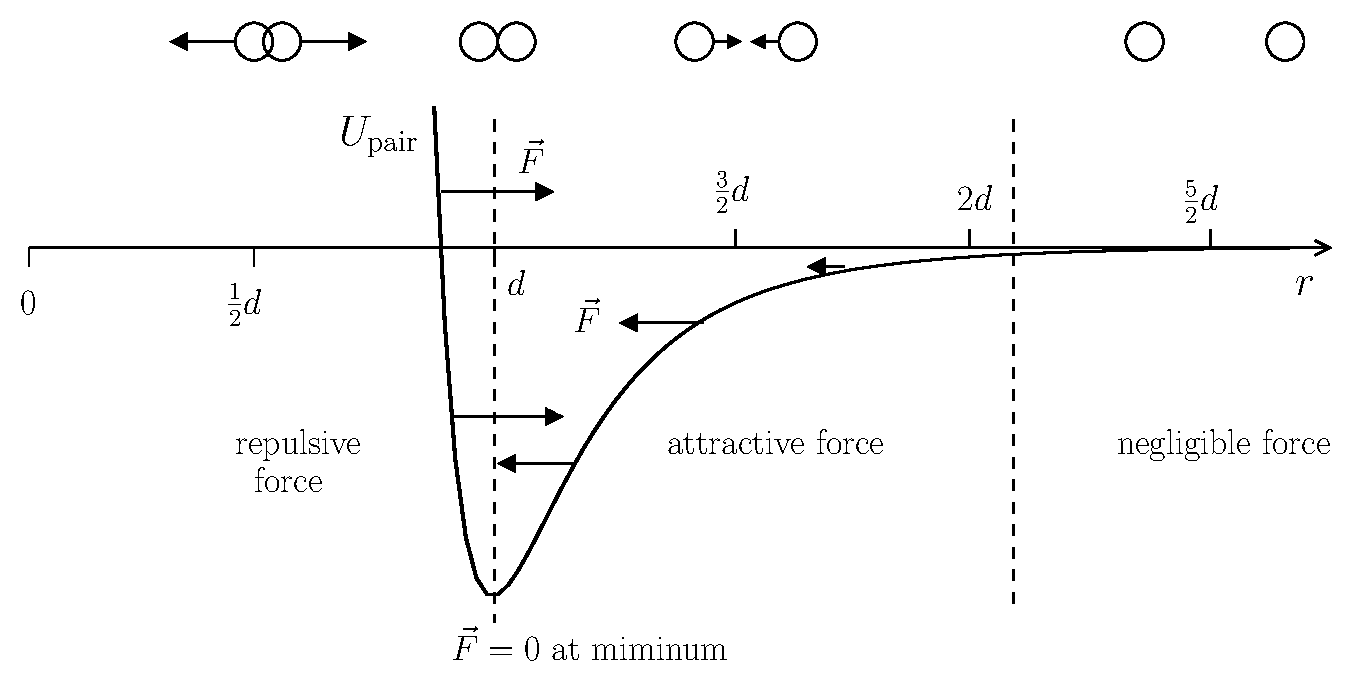
\includegraphics[width=5in]{thermal_energy_and_solids/pair_potential.eps}
\caption{The pair potential energy $U_\text{pair}$ as a function of
  $r$, the separation between the pair of molecules.  The dashed lines
  separate the regions of repulsive force, attractive force, and
  negligible force.  At separation $r=d$ the pair is in equilibrium,
  which defines the molecular diameter.}
\label{fig:pair_potential}
\end{center}
\end{figure}

What about other sources of potential energy besides the
intermolecular forces?  For example, gravitational potential energy.
When a ball is thrown upwards, the gravitational potential energy of
each molecule increases.  But the height of each molecule is increased
by the same amount that the height of the center of mass is increased.
Therefore this change in potential energy has the form
\begin{equation}
\Delta U_\text{grav} = M_\text{object} g\Delta y_{cm},
\end{equation}
where $M_\text{object}$ is again the total mass of the object.  This
is the familiar mechanical potential energy.  Therefore, gravitational
potential energy is always part of the mechanical energy, whereas the
molecular interaction energy makes up the thermal potential energy.

In summary, here is the big picture for thermal energy:
\begin{itemize}
\item For both potential energy and kinetic energy, it is the
  `organized' motion that makes up the {\it mechanical energy}, such as
  all molecules increasing their height together or all molecules
  having a net alignment of their velocities.
\item The remaining disorganized motion, such as the wiggling of the
  mole\-cules and their individual pushes and pulls on each other,
  corresponds to the {\it thermal energy}.
\item Friction is an agent that takes organized motion and
  disorganizes it, taking away mechanical energy and increasing thermal
  energy.
\item Going the other way --- taking away thermal energy and
  increasing mechanical energy --- is more difficult, since molecules
  are not likely to spontaneously start moving together.
  Nevertheless, we can capture some amount of thermal energy and
  convert it to mechanical energy with a device called a heat engine,
  which is the topic of Supplementary Reading Chapter
  \ref{chapter:heat_engines}.
\end{itemize}

\section{The Solid State}

\label{section:the_solid_state}

Molecules interacting via the pair potential can be solids, liquids,
or gases.  The remainder of this chapter is concerned with the thermal
energy of the solid state, while liquid and gas states will be
presented in Chapter \ref{chapter:liquids_and_gases}.


Most inorganic solids are crystalline, which means the molecules are
arranged in a symmetric way, such as a cubic lattice.  (Organic
  solids instead are constructed from long carbon chains.)  In this
lattice, each pair of neighboring molecules is separated by roughly
the equilibrium distance, that is, the minimum of the pair potential
well, and only makes small excursions from this location.  As
illustrated in Fig.~\ref{fig:pair_potential_spring}, the pair
potential in this region is identical to a parabolic potential.  We
have previously encountered a parabolic potential energy curve as the
potential energy for a mass on a spring.  Evidently, as long as the
molecules in a solid are not deviating significantly from their
equilibrium position, we may regard their interactions with their
nearest neighbors as equivalent to being attached by a spring.

\boxittext{{\sc Checkpoint:} What is the main difference between the pair
  potential and the spring potential?  What would I need to do to a
  pair of molecules to see this difference?  (Push together?  Pull
  apart?  How far?) }

\begin{figure}
\begin{center}
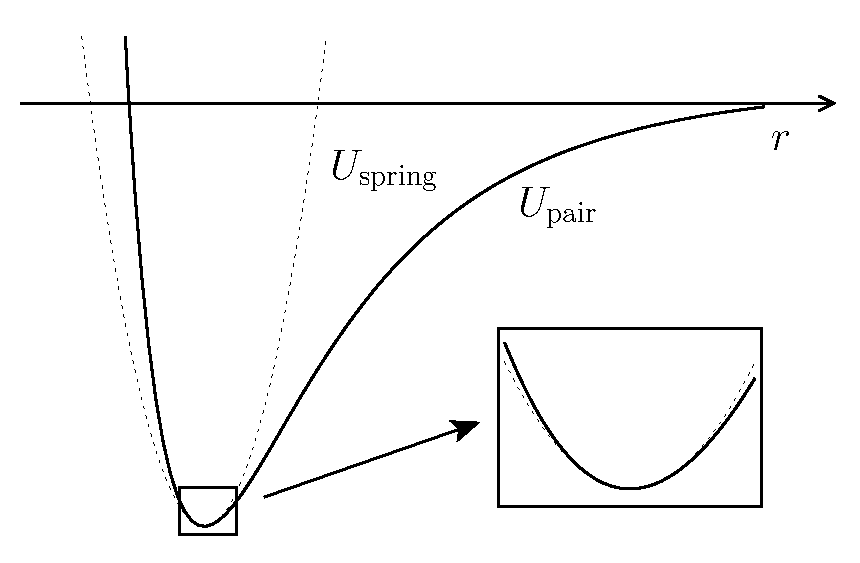
\includegraphics[width=3.5in]{thermal_energy_and_solids/pair_potential_spring.eps}
\caption{The solid curve is the pair potential $U_\text{pair}$ as a
  function of separation $r$.  The dashed line is the spring potential
  $U_\text{spring}$ with the spring constant $k_{\text sp}$ chosen to match
  $U_\text{pair}$ near the minimum.  The inset shows the match.}
\label{fig:pair_potential_spring}
\end{center}
\end{figure}


This leads to what we call the {\it ideal solid}:
the molecules are balls of mass $m$, they are connected by springs of
spring constant $k_\text{sp}$, and the springs have an equilibrium length
of $d$.  This model is illustrated in Fig.~\ref{fig:ball-spring}.  We
may think of the spring constant as determining the bond strength and
the equilibrium length $d$ as the bond length.  These three parameters
($m$, $d$, and $k_\text{sp}$) define the model, and we shall see that for
many solids determining these parameters describes much of the
behavior of the solid.

One may imagine packing the molecules together in different ways.  The
arrangement illustrated in Fig.~\ref{fig:ball-spring}, is called a
{\it simple cubic} lattice.  In fact, most solids are packed
differently, for example, in the way a grocer would stack oranges
(which is called a {\it face-centered cubic} lattice).  Fortunately,
this distinction has little impact on the quantities we will study, so
we will stick with the simple cubic lattice.

\begin{figure}
\begin{center}
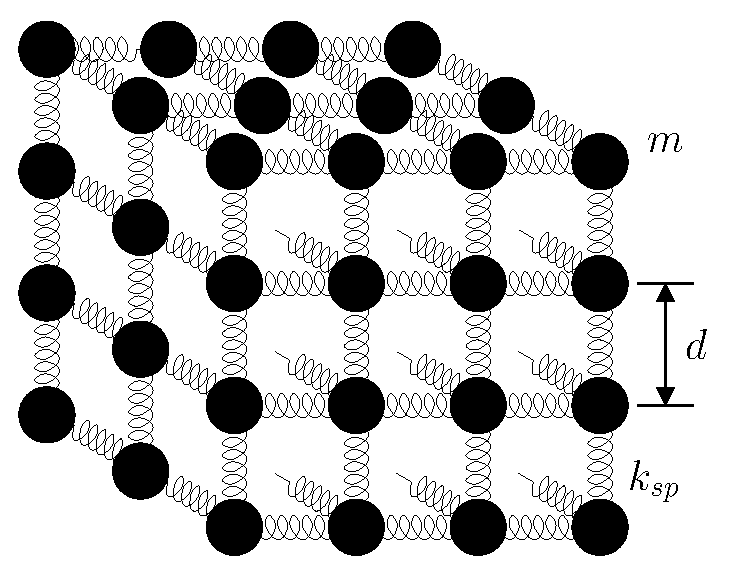
\includegraphics[width=2.5in]{thermal_energy_and_solids/ball-spring.eps}
\caption{The ball-spring model of a solid.}
\label{fig:ball-spring}
\end{center}
\end{figure}

Given the properties of some solid, how are the ideal solid
parameters determined?  Let's derive these for a specific case, namely
copper.  Molecular properties, such as mass, are usually not specified
for a single molecule, but rather for a {\it mole}.  One mole equals
Avogadro's number
\begin{equation}
N_A=6.02\times 10^{23}
\end{equation} 
of molecules.  Avogadro's number is chosen so that roughly one mole of
protons has a mass of one gram.  The precise definition is that one
mole of carbon atoms has a mass of $12\units{g}$.  The mass of one mole
of a material would logically be called the molar mass, but instead it
is usually called the {\it molecular weight}.\footnote{It's not our fault.}

One mole of copper has mass $64\units{g}$, so we may conclude that a
single molecule of copper (the ball in our model) has mass
\begin{equation}
m_\text{Cu} = \frac{64\units{g}}{6.02\times 10^{23}} = 1.06\times
10^{-22}\units{g}.
\end{equation}
This is the first of our three parameters.

Next, we can get the equilibrium spacing $d$ between the molecules by
knowing the density of copper, which is $8.94\units{g/cm$^3$}$.  
In Fig.~\ref{fig:ball-spring-volume} shows that each molecule of copper
occupies its own cubical region with volume $d^3$.
We can relate the density $\rho$ of the solid to the mass per volume
of a unit cell.  That is,
\begin{equation}
\rho = \frac{\text{mass}}{\text{volume}} = \frac{m}{d^3} 
  \qquad \Rightarrow\qquad d =
\left(\frac{m}{\rho}\right)^{1/3}.
\end{equation}
For copper this gives
\begin{equation}
d_\text{Cu} = \left(\frac{m_\text{Cu}}{\rho_\text{Cu}}\right)^{1/3}
 =  \left(\frac{1.06\times
     10^{-22}\units{g}}{8.94\units{g/cm$^3$}}\right)^{1/3}
 = 2.28\times 10^{-8}\units{cm},
\end{equation}
or equivalently, $2.28\times 10^{-10}\units{m}$.
And so we have the second parameter.

%Next, we can get the equilibrium spacing between the molecules by
%knowing the density of copper, which is $8.94\units{g/cm$^3$}$.  How
%many copper molecules are in a cubic centimeter of copper?    We can 
%calculate this as follows:
%\begin{equation}
%\frac{8.94\units{g}}{64\units{g/mole}} = 0.139 \units{mol}
% = 8.41\times 10^{22} \units{molecules},
%\end{equation}
%where Avogadro's number was used to convert moles to molecules.  The
%cubic centimeter of volume is divided equally among this number of
%molecules so the volume per molecule is
%\begin{equation}
%\frac{1 \units{cm$^3$}}{8.41\times 10^{22}\units{molecules}}
% = 1.19\times 10^{-23}\units{cm$^3$}.
%\end{equation}
%
%The volume for a single molecule can be pictured as a cube of length
%$d$, where $d$ is the bond length (see
%Fig.~\ref{fig:ball-spring-volume}).  Since the volume of a cube is
%$V=d^3$, the bond length is obtained from $d=V^{1/3}$, or
%\begin{equation}
%d = (1.19\times 10^{-23}\units{cm$^3$})^{1/3} = 2.28\times 10^{-8}\units{cm}
% = 2.28\times 10^{-10}\units{m}.
%\end{equation}
%And so we have the second parameter.

\begin{figure}
\begin{center}
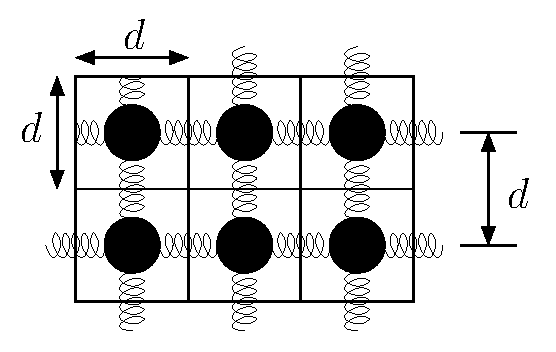
\includegraphics[width=2in]{thermal_energy_and_solids/ball-spring-volume.eps}
\caption{For the ideal solid with a separation $d$ between the 
balls, the volume per ball is given by a cube of side $d$ (shown here
in two-dimensions).}
\label{fig:ball-spring-volume}
\end{center}
\end{figure}


The final step is to determine the spring constant.  Fortunately, it
is not necessary to try pulling on a single molecule and measuring the
force that it pulls back with.  Rather, a macroscopic chunk of
material can be fixed at one end and pulled on the other, and by
measuring how much the object stretches, the bond spring constant can
be measured.

Imagine a piece of copper wire with cross-sectional area $A$ and
length $L$.  The applied force required to stretch the wire by an amount
$\Delta L$ is given by the following relation:
\begin{equation}
F_\text{app} = \frac{Y A}{L}\Delta L.
\label{eq:force_extension}
\end{equation}
This relation indicates that the amount of stretch $\Delta L$ is
proportional to the amount of force applied; doubling the force will
double the amount of stretch from the equilibrium length.  A larger
cross-sectional area $A$ makes the wire harder to stretch, which
accounts for the factor of $A$ in the numerator.  The longer the wire,
the easier it is to stretch, accounting for the factor of $L$ in the
denominator.  The final parameter $Y$ is called Young's modulus,
and is a property of the material but not dependent on the geometry
of the wire.  For example, Young's modulus for copper is
$Y_\text{Cu} \approx 130\times 10^9 \units{N/m$^2$}$.  

\begin{example}{Stretching an Extension Cord}
Consider 16 gauge copper wire, commonly used in power cables, which 
has a
cross-sectional area of $1.3\times 10^{-6}\units{m$^2$}$.  How much
force is required to stretch a 2-meter length of wire a distance of
1 centimeter?
\solution
According to Eq.~(\ref{eq:force_extension}), the force is given by
\begin{align}
 F_\text{app} = \frac{Y_\text{Cu}A}{L}\Delta L &=
 \displaystyle\frac{(130\times 10^9\units{N/m$^2$})(1.3\times
  10^{-6}\units{m$^2$})} {2\units{m}} (0.01\units{m}) \nonumber\\
 &= 845\units{N}.
\end{align}
\end{example} 

Now we need to calculate Young's modulus for the ideal solid.
Consider a rectangular solid of $N_x \times N_y \times N_z$ molecules.
The object is stretched in the $z$-direction by an applied force $F$,
with a resulting stretch $\Delta L$.  The stretch is shared equally
among each of the $N_z$ springs aligned in the $z$-direction, so each
spring is stretched an amount $\Delta L/N_z$.  The plane of molecules
where the force is applied consists of $N_xN_y$ molecules, each
connected to a spring pulling with force $k_\text{sp}\Delta L/N_z$.  This
spring force is balancing the applied force, so we can conclude that
\begin{equation}
F_\text{app}= N_xN_y \left(\frac{k_\text{sp} \Delta L}{N_z}\right).
\end{equation}
If we multiply top and bottom by $d^2$ we can identify the
cross-sectional area $A=(N_x d)(N_y d)$, and the length $L=N_z d$:
\begin{equation}
F_\text{app}=\frac{d^2N_xN_y k_\text{sp}}{d^2 N_z} \Delta L 
                = \frac{k_\text{sp}}{d}
\frac{A}{L}\Delta L
\end{equation}
from which we conclude that Young's modulus for the ideal solid
is
\begin{equation}
Y=\frac{k_\text{sp}}{d}.
\end{equation}
This can be used to find the spring constant, $k_\text{sp} = Yd$.  For
example, for copper
\begin{equation}
k_\text{sp} = (130\times 10^9\units{N/m$^2$})(2.28\times 10^{-10}\units{m})
 = 29.6\units{N/m}.
\end{equation}
In this way, we can find all three ideal solid parameters from
knowing the molecular weight, the density, and Young's modulus.


\section{Speed of Sound}
\label{section:speedofsound}

How well does this ball-spring picture of a solid work? 
One way to test the model is to study the speed of sound in a
solid.  Sound is a compression wave, much like a compression pulse
sent down a stretched slinky.  If an ideal solid is suddenly
struck at one end, how fast does the compression wave travel toward
the other end?  We can almost guess the answer.  The wave ``hops''
from one molecule to its neighbor and each hop moves the wave a
distance $d$.  Since the molecules are harmonic oscillators, the time
it takes for a hop must be related to the period of oscillation $T$,
so we could guess $v_\text{sound} \approx d/T$.  It is not difficult
to do the full calculation for the ideal solid\footnote{This is
  done in PHYS 221/222.} and find that the answer differs from this
guess by a factor of $2\pi$:
\begin{equation}
v_\text{sound} = \frac{2\pi d}{T} = d\omega  = d\sqrt{\frac{k_\text{sp}}{m}}
\end{equation}
Thus, the speed of sound in the ideal solid depends on all three
parameters.  The values we obtained for copper (be careful to use SI
units here!) give
\begin{equation}
 v_\text{sound} = 2.28\times
 10^{-10}\units{m}\sqrt{\frac{29.6\units{N/m}}{1.06\times
     10^{-25}\units{kg}}} = 3810\units{m/s}
\end{equation}
which is exactly the measured value for the speed of sound in copper.
Evidently the ideal solid model works quite well.  You will make more
comparisons in the homework.

\section{Temperature}

We began the chapter mentioning that when mechanical energy gets
converted to thermal energy, the temperature increases.  But what is
temperature?  Everyone has an intuitive feel for it:  we know that a
high temperature corresponds to something that is ``hot'' and a low
temperature corresponds to something that is ``cold.''  We also know
from experience that ``heat'' --- which we will define shortly --- flows
from hot (high temperature) to cold (low temperature) objects.

It is common in many introductory text books to define temperature as
a measure of the average thermal kinetic energy $K_\text{therm}/N$ of
a material.\footnote{Historically, this approach was used successfully
  in the $18^\text{th}$ and $19^\text{th}$ centuries to develop the
  first successful quantitative theories of thermodynamics, referred
  to as the {\em kinetic theory} of thermodynamics.}  This definition of
temperature is not valid for all situations (we will provide a more
rigorous definition of temperature in Chapter
\ref{chapter:second_law}); however, there are many situations that can
benefit from simple view of temperature as a measure of thermal
kinetic energy.

We must talk about temperature units.  The Celsius
temperature scale is defined so that water freezes at a temperature of
$0^\circ\units{C}$ and water boils at $100^\circ\units{C}$.  Considering
temperature as a measure of kinetic energy, we can define {\em absolute
zero} as the temperature where all molecular motion stops.  This occurs at
$-273.15^\circ\units{C}$ in the Celsius scale.  

\begin{figure}
\begin{center}
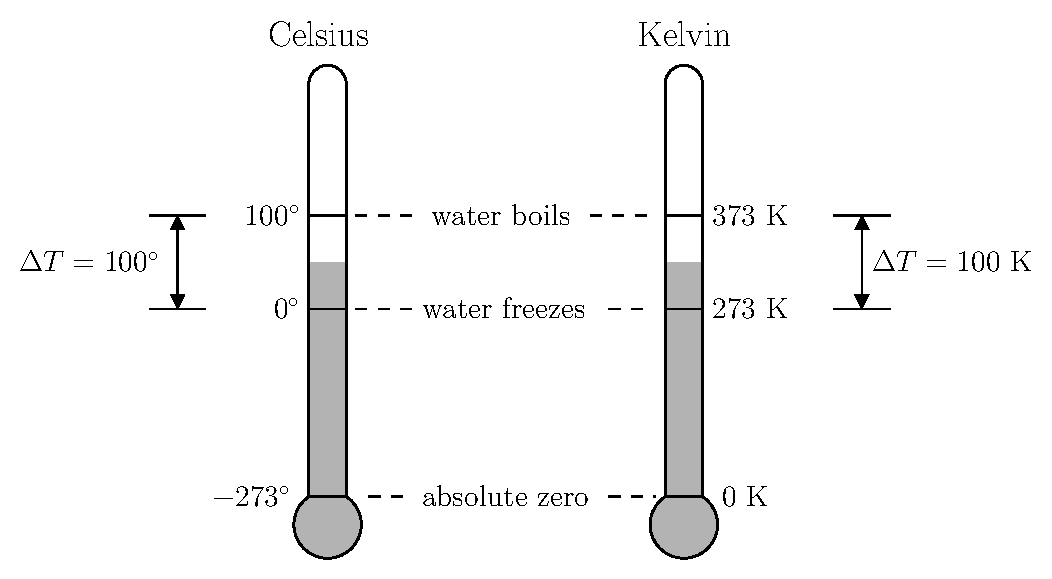
\includegraphics[width=4.5in]{thermal_energy_and_solids/temperature_scales}
\caption{The size of the degree is the same for Celsius and Kelvin
  temperature scales.  They differ by a shift:  $T_K=T_C+273$}
\label{fig:temperature_scales}
\end{center}
\end{figure}

A important variation on the Celsius temperature scale is called the
Kelvin scale, illustrated in Fig.~\ref{fig:temperature_scales}.  The
``size'' of the degree is the same for Kelvin and Celsius, that is, a
change in temperature of $1\units{K}$ is the same as a change in
temperature of $1^\circ\units{C}$.  The boiling temperature of water
is still $100\units{K}$ higher than the freezing temperature. The
difference in the scales is the location of zero: in the Kelvin scale,
absolute zero corresponds to $0\units{K}$, water freezes at
$273\units{K}$ and boils at $373\units{K}$.  The Kelvin temperature
scale is the one best suited for most thermodynamics problems.


\section{Molar Specific Heat}

Now we are prepared to address the question, ``If a certain amount of
thermal energy is added to a system, how much will the temperature
increase?''  This is a question with far-reaching applications.  For
instance, how much energy needs to be added to a swimming pool to heat
it up to a comfortable temperature?  How much cooling water or antifreeze
is needed to keep a car from overheating?  How much will the temperature
of a bucket of water increase if a hot ingot of lead is tossed into it?

We mentioned in the previous section that temperature is often associated
with the thermal energy of a system, i.e., increases in temperature
are associated with increases in the thermal energy.  But {\em how much}
does the temperature increase with a certain amount of energy is
added to a material?  For that, we define the {\em molar specific heat}
$C$:
\begin{equation}
C = \frac{\Delta E_\text{therm}}{n \Delta T}.
\label{eq:specificheat}
\end{equation}
In words, the specific heat is defined as the energy required to
raise the temperature of one mole of a material by a temperature 1 K.
So, a material with a large specific heat requires a lot of heat to
increase its temperature significantly, whereas a material with a
small specific heat requires less energy to raise its temperature by the
same amount.

Turning Eq.~(\ref{eq:specificheat}) around, the energy
required to raise the temperature of a material is given by
\begin{equation}
\Delta E_\text{therm} = n C \Delta T.
\label{eq:Ethermspecificheat}
\end{equation}
Measurements have been made of the molar specific heat for a wide
variety of materials.  A few of these values are listed in 
Table~\ref{table:material_properties} for some common metals.  

Note that the relation between the thermal
energy and the temperature depends on the amount of material via the
number of moles $n$. Having more stuff
will require more thermal energy to get the same temperature change.
The molar specific heat $C$, however, is defined such that it
does {\it not} depend on the amount of material.

\newpage

\begin{example}{Temperature increases}
How much thermal energy must be added to $5.0\units{kg}$ of lead to
increase its temperature from $25^{\circ}\units{C}$ to $40^{\circ}\units{C}$?

\solution First, it is convenient to determine how many moles of lead
we have here.  From Table~\ref{table:material_properties}, we see that
the molar mass of lead is $207\units{g/mol}$, so the number of moles
is given by
\begin{equation*}
n = 5.0\units{kg} \cdot \frac{1000\units{g}}{\units{kg}} \cdot 
\frac{1\units{mol}}{207\units{g}} = 24.2\units{mol}
\end{equation*}
From Table~\ref{table:material_properties}, we see that
the molar specific heat of lead is 
$26.6\units{$\frac{\rm J}{\rm mol} \cdot {\rm K}$}$.
Using Eq.~(\ref{eq:Ethermspecificheat}), we find
\begin{equation*}
\Delta E_\text{therm} = n C \Delta T = 24.2\units{mol} \cdot
26.6\units{$\frac{\units{J}}{\units{mol} \cdot \units{K}}$} \cdot 15\units{K} = 9640\units{J}.
\end{equation*}
Note that the conversion between Celsius and Kelvin is trivial; a
temperature difference of $15^{\circ}\units{C}$ is the same as a
temperature difference of $15\units{K}$.
\end{example}

Looking at Table~\ref{table:material_properties}, it is apparent that
the molar specific heat for metals is fairly consistent --- around 
$25\units{J/mol$\cdot$K}$ --- for several common metals.  A pattern like this
indicates that there might be a simple, common explanation.  That
explanation is provided by the ideal solid model and what is known as the
equipartition theorem.

\section{The Equipartition Theorem}
\label{sec:equipartition}

We now discuss a remarkable relationship between temperature and
thermal energy, referred to as the {\em equipartition theorem}.  The
basic idea is that in thermodynamic systems, thermal energy is equally
(``equi'') divided (``partition'') between certain types of molecular
energy, both kinetic and potential.  At first glance, you might think
that this would mean that half of the energy is kinetic and half is
potential (and sometimes this is true), but it is not quite that simple.
For one, only those energy terms which are quadratic in a
dynamical variable (such as $\frac{1}{2}mv_x^2$) get the equal shares.
For any terms more complicated than that, like the pair potential, we
cannot so easily say how the energy is divided.  Also, the number of these
egalitarian quadratic energy terms, often called {\it degrees of freedom},
depends on details such as whether there is rotational as well as
translational kinetic energy.\footnote{For a solid the molecules
  essentially do not rotate, but rotational kinetic energy can have a
  significant effect on the thermal energy of a liquid or gas.}


% because (a) there are different types of kinetic
%energy, e.g., translation and rotational\footnote{For a solid the
%molecules essentially do not rotate, but rotational kinetic energy
%  can have a significant effect on the thermal energy of a liquid
%  or gas.} kinetic energy; (b) the partition of energy also depends on
%the number of {\em degrees of freedom} a system has, e.g., whether a
%molecule can oscillate only in one direction (1 degree of freedom),
%along a plane (2 degrees of freedom) or in any of the three dimensions
%(3 degrees of freedom); and (c) it only applies to {\em quadratic}
%degrees of freedom, meaning the energy term has to be proportional to
%the variable squared.

Maybe it will help to see the theorem:

\boxittext{{\sc Equipartition Theorem:}\\[0.5ex]
  Any term in the energy of a
  molecule that is quadratic, such as $\frac{1}{2}mv_x^2$ or
  $\frac{1}{2}k_\text{sp}x^2$ or $\frac{1}{2}I\omega^2$, averages to
  $\frac{1}{2}k_BT$.}

This amazing result says that when some $10^{23}$ particles push and pull
and collide with each other, all the messy forces involved will result in
every quadratic energy term averaging to the same value.   It doesn't
matter if the molecule is heavier or lighter, or what the spring
constant is.  It also doesn't matter whether we are talking about
potential energy or translational kinetic energy or rotational kinetic
energy.  As long as the energy is quadratic in the dynamical variable, 
the thermal energy will depend only on $T$ and
Boltzmann's constant,
\begin{equation}
k_B= 1.38\times 10^{-23}\units{J/K},
\end{equation}
which is another constant of nature.  Notice how the units work out:
$k_BT$ is an energy.

%As an example, let's say that we have a gas composed of N non-interacting
%atoms (i.e., neglecting any forces between them), each of which 
%can move in the $x-$, $y-$ or $z-$directions.
%The energy of one of these atoms is then
%\begin{equation*}
%E_\text{atom} = 
%{\textstyle\frac{1}{2}}mv_x^2 +
%{\textstyle\frac{1}{2}}mv_y^2 +
%{\textstyle\frac{1}{2}}mv_z^2.
%\end{equation*}
%(There are no potential energy terms here because we are neglecting
%interactions between the atoms.)
%According to the equipartition theorem, each of these three terms
%averages to ${\textstyle\frac{1}{2}}k_BT$, so the average energy
%per atom is
%\begin{equation*}
%\langle E_\text{atom}\rangle = 3\left({\textstyle\frac{1}{2}}k_BT\right) 
%= {\textstyle\frac{3}{2}}k_BT.
%\end{equation*}
%and the total thermal energy for the system is simply
%\begin{equation*}
%E_\text{therm,gas} = N ({\textstyle\frac{3}{2}}k_B T)
%\label{eq:E_thermalgas}
%\end{equation*}
%Note how quick this result is.  We don't have to worry about any of
%the details of the individual atoms in the gas.  The equipartition
%theorem takes care of all of that for us.

In the next sections, we'll use the equipartition theorem to analyze
thermal energy of an ideal solid.

\section{Ideal Solid Specific Heat}

To determine the molar specific heat of an ideal solid,
let us make the approximation that the neighbors of
a particular molecule remain fixed.  This turns out to be a reasonable
approximation for most solids.  Then the energy describing that
particular molecule is
\begin{equation}
E_\text{molecule} = {\textstyle\frac{1}{2}}mv_x^2 +
{\textstyle\frac{1}{2}}mv_y^2 + {\textstyle\frac{1}{2}}mv_z^2 +
{\textstyle\frac{1}{2}}k_\text{sp}x^2 + {\textstyle\frac{1}{2}}k_{\rm sp}y^2 +
{\textstyle\frac{1}{2}}k_\text{sp}z^2.
\label{eq:ball-spring_energy}
\end{equation}
There are six terms contributing to the energy, all of which are
quadratic.  Each term is fluctuating up and down as the molecule
interacts with its neighbors.  The equipartition theorem tell us,
then, that the average energy of this ball over time will be
\begin{equation}
\langle E_\text{molecule}\rangle =
6\left({\textstyle\frac{1}{2}}k_BT\right) = 3k_BT.
\end{equation}
Now consider an $N$ molecule ideal solid.  The number of moles
is given by $n = N/N_A$, and the 
thermal energy will be
\begin{equation}
E_\text{therm} = N (3 k_B T) = \frac{N}{N_A}(3k_BN_A)T = n3RT,
\quad\text{(ideal solid)}
\label{eq:E_thermal}
\end{equation}
where $R=N_A k_B = 8.31\units{J/mol$\cdot$K}$ is called the gas
constant, although it has nothing in particular to do with
gases.\footnote{This isn't our fault either.}  

Comparing Eqs.~(\ref{eq:E_thermal}) and (\ref{eq:Ethermspecificheat}),
the molar specific heat of the ideal solid is
\begin{equation}
C = 3R = 24.9\units{J/mol$\cdot$K} \qquad\text{(ideal solid)}
\end{equation}
regardless of the material.  This relation is known as the
Dulong-Petit law.  The molar specific heats of most solids agree with
the Dulong-Petit result to within a few percent accuracy.  For
example, the molar specific heat of copper is $C_\text{Cu} =
24.4\units{J/mol$\cdot$K}$, and comparable values for a variety of
other solids are given in Table~\ref{table:material_properties}.  This
provides more evidence that the ball-spring model of the ideal solid
is reasonable.


\begin{table}
\begin{tabular}{lccccc}
\hline\hline
Material & $M$ (g/mol) & $\rho$ (g/cm$^3$) & $Y$ (GN/m$^2$) & 
$C$ (J/mol$\cdot$K)  & $v_s$ (m/s) \\ \hline
% & (g/mol) & (g/cm$^3$) & (GN/m$^2$) & (J/mol$\cdot$K) & (m/s)\\ \hline
Aluminum & 27.0 & 2.70 & 70  & 24.2  & 5000\\
Iron     & 55.8 & 7.87 & 211 & 25.1  & 5120\\
Copper   & 63.5 & 8.96 & 130 & 24.4  & 3810\\
Gold     & 197  & 19.3 & 78  & 25.4  & 2030\\
Lead     & 207  & 11.3 & 16  & 26.6  & 1190\\
ideal solid & $mN_A$ & $m/d^3$ & $k_{\rm sp}/d$ & 3R = 24.9  
                                          &  $d\sqrt{k_{\rm sp}/m}$\\
\hline\hline
\end{tabular}
%\caption{Material properties for a few selected substances.}

% \begin{tabular}{lccccc}
% \hline\hline
% Material & $M$ (g/mol) & $\rho$ (g/cm$^3$) & $Y$ (GN/m$^2$) & 
% $C$ (J/mol$\cdot$K)  & $v_s$ (m/s) \\ \hline
% % & (g/mol) & (g/cm$^3$) & (GN/m$^2$) & (J/mol$\cdot$K) & (m/s)\\ \hline
% Aluminum & 27.0 & 2.70 & 70  & 24.2  & 5000\\
% Iron     & 55.8 & 7.87 & 211 & 25.1  & 5120\\
% Copper   & 63.5 & 8.96 & 130 & 24.4  & 3810\\
% Gold     & 197  & 19.3 & 78  & 25.4  & 2030\\
% Lead     & 207  & 11.3 & 16  & 26.6  & 1190\\
% ideal solid & $mN_A$ & $m/d^3$ & $k_\text{sp}/d$ & 3R = 24.9  
%                                           &  $d\sqrt{k_\text{sp}/m}$\\
% \hline\hline
% \end{tabular}
\caption{Material properties for a few selected substances.}
\label{table:material_properties}
\end{table}

Finally, note that the specific heat is only defined in terms of
$\Delta E_\text{therm}$ and $\Delta T$; it relates {\it changes} in
the temperature to changes in thermal energy.  However, if we assume
that the specific heat is independent of temperature, which is a
reasonable approximation down to some low temperature, then we can
also estimate
\begin{equation}
E_\text{therm} \approx nCT = n3RT. \qquad\text{(ideal solid)}
\end{equation}


\section{Heat and the First Law of Thermodynamics}
\label{section:heat}

There are many ways to add thermal energy to an object or to remove it
from the object.  We have already discussed how friction can increase
the thermal energy of a blow dart as it slides across the floor.
Another way to change the thermal energy is to bring the object into
{\it thermal contact} with something hotter or colder.  For a pair of
solid objects, thermal contact occurs when they are physically in
contact.  Then the molecules at the boundary exert forces on each
other and energy is transferred from the object with the higher
temperature to the object with the lower temperature.  
As we have already discussed,  temperature directs the flow of
thermal energy, determining which objects will spontaneously give off
energy and which objects will receive it.

The energy transferred spontaneously by molecular motion is given the
name {\it heat.}  Similar to work, heat is an energy transfer and not
an energy.  Think of thermal energy as a bank balance and heat and work
as deposits and withdrawals.  The distinction between heat and
work is the mechanism for the energy transfer.

\boxittext{Heat is the thermal energy transferred spontaneously due
to a temperature difference.}

\noindent All other forms of energy transfer into a system are lumped 
together as thermodynamic ``work."  For example, the term work can refer 
to energy transfer due to external forces that act on system (but do not 
change the motion of the center of mass of the system)\footnote{In Unit 1 
in this course we discussed the work done on a single particle,
and the resulting change in the kinetic energy of the particle.
In thermodynamics we are interested in composite systems, such as gases
liquids, and solids.  In composite systems, work can result in changes in
thermal energy as well as kinetic energy. In the thermodynamic systems
we study, there will be no changes in the bulk kinetic energy 
$K_\text{mech}$.}, but it also 
encompasses energy transfers due to other things, such as the warming of 
a piece of frozen broccoli in a microwave oven.  To distinguish the 
two forms of energy transfer, it is common to use the symbol $Q$ for heat, 
and $W$ for work.

Now we can state the first law of thermodynamics, which is simply a
statement of energy conservation: the change in thermal energy is
equal to how much work is done on the system plus how much heat flows
into the system:
\begin{equation}
\Delta E_\text{therm} = Q + W \qquad\text{(1st Law of Thermodynamics)}
\end{equation}
Note that $Q$, like $W$, can be positive or negative, depending on
whether heat is flowing in or out.  The convention used here is to
define the heat $Q$ as being positive if heat is flowing {\em into}
the material (and negative if heat is flowing out), and to define
the work $W$ as the work done {\em on} the system.  Some people find it
convenient to write the first law with these conventions stated
explicitly:
\begin{equation}
\Delta E_\text{therm} = Q_\text{in} + W_\text{on} \qquad\text{(1st Law of Thermodynamics)}
\label{eq:firstlaw}
\end{equation}

From our perspective today, with energy conservation a fundamental
principle, the 1st law may seem to be pretty obvious.  But historically it was a
very significant discovery, showing that indeed heat was just an
energy transfer, rather than some new substance.\footnote{Early theories of
thermodynamics proposed -- incorrectly -- that heat was some sort of
fluid (called {\em caloric}) that flows between hot and cold materials.
We now know, of course, that heat is simply the ``flow'' of energy.}
And the
importance of the first law cannot be overstated -- this seemingly simple
result forms the foundation of much of what we will be doing during
the next couple of weeks.

It is worth appreciating what is not heat.  Rubbing your hands
together when they are cold certainly does increase their thermal
energy, but not due to heat.  There is not a higher temperature object
making energy flow into your hands spontaneously, so there is no heat
flow.  Rather, you are doing work with your muscles, and the friction
force between your hands converts the mechanical energy of your moving
hands into thermal energy.

\begin{example}{First law}
You hold a $35\units{mol}$ iron anvil in place on a moving conveyor belt
so that the belt slides under the stationary anvil. The belt does 
$12,000\units{J}$ of work on the anvil, and and it gets warmer. During 
this process, the anvil loses $7,000\units{J}$ to the cooler surrounding air 
and to the belt.  If the anvil had an initial temperature of 
$22.0^{\circ}\units{C}$, what is its temperature at the end of this 
process?

\solution
First, we can use the first law to determine the change in the anvil's
thermal energy.  Conceptually, $12,000\units{J}$ is  added in the form
of work and $7,000\units{J}$ is removed in the form of a heat flow.  In terms
of Eq.~(\ref{eq:firstlaw}), $W_\text{on}=12000\units{J}$ and 
$Q_\text{in}=-7000\units{J}$ (negative since heat is flowing {\em out}
of the anvil).  So,
\begin{equation*}
\Delta E_\text{therm} = Q_\text{in} + W_\text{on} 
     = -7000\units{J} + 12000\units{J}= 5000\units{J}.
\end{equation*}
We can now use Eq.~(\ref{eq:Ethermspecificheat}) and the molar specific
heat of iron (see Table~\ref{table:material_properties} to find the
temperature change of the iron anvil:  
\begin{equation*}
\Delta E_\text{therm} = n C \Delta T.
\end{equation*}
Solving for the rise in temperature gives
\begin{eqnarray*}
\Delta T &=& \frac{\Delta E_\text{therm}}{nC} \\
         &=& \frac{5000\units{J}}{35\units{mol} \times 25.1\frac{\units{J}}
{\units{mol} \cdot \units{K}}} \\
         &=& 5.7\units{K}
\end{eqnarray*}  
The final temperature is therefore $22.0^\circ\units{C} + 5.7^\circ\units{C} = 
27.7^\circ\units{C}$.


Note that we could get a very good approximation of the result here by using
the ideal solid approximation for the molar
specific heat.

\end{example}


When a pair of objects is in thermal contact but is otherwise thermally
isolated, we can say that $\Delta E_\text{therm}$ is equal and opposite
for the two objects, since the thermal energy lost by the hotter object
is gained by the colder object.  This brings the objects closer together
in temperature, until finally they have the same temperature and no more
heat flows.  This situation is called {\it thermal equilibrium}.

\begin{example}{Hot Meets Cold}
One mole of an ideal solid at temperature $70^\circ\units{C}$ is
brought into thermal contact with two moles of an ideal solid at
temperature $10^\circ\units{C}$.  How much heat will flow out of the
hotter object before thermal equilibrium is reached?
 
\solution 
We will need to
determine the final equilibrium temperature, $T_f$.  
This is done by balancing the heat flows in and out:
\begin{equation} 
\Delta
E_\text{therm,1} = -\Delta E_\text{therm,2} 
\>\Rightarrow\>
n_1 C_1 \underbrace{(T_f - T_{1,i})}_{\Delta T_1} = -n_2 C_2 
\underbrace{(T_f - T_{2,i}) }_{\Delta T_2}
\label{eq:calorimetry}
\end{equation}
where $T_{1,i}$ and $T_{2,i}$ are the initial temperatures of objects
1 and 2.  Putting in values:
\begin{equation}
(1\units{mol})(3R)(T_f - 70^\circ\units{C})
 = -(2\units{mol})(3R)(T_f - 10^\circ\units{C})
\end{equation}
Note that we have used Celsius temperature.  This is because $\Delta
T$ is the same whether measured in Kelvin or Celsius (see
Fig.~\ref{fig:temperature_scales}).  Now we solve:
\begin{equation}
T_f - 70 = -2(T_f-10)\quad\Rightarrow\quad 3T_f = 70+20
\end{equation}
so
\begin{equation}
T_f = \frac{90}{3} = 30^\circ\units{C}.
\end{equation}
To complete the calculation, we go back to the change in thermal energy,
Eq.~(\ref{eq:calorimetry}),
\begin{equation}
\Delta E_\text{therm,1} = (1\units{mol})(24.9\units{J/mol$\cdot$K})
(30^\circ\units{C} - 70^\circ\units{C}) = -996\units{J}.
\end{equation}
So $996\units{J}$ of heat flowed out of object $1$ and into object $2$.
\end{example}



\newpage

\section*{Problems}
\markright{PROBLEMS}

\begin{problem}
  To understand better how the ideal solid thermal energy
  is derived, consider the following scenario.
  A mad scientist creates a new material, flattium, in which the
  molecules can only move in the $x$-$y$ plane, while their $z$
  coordinates remain fixed.  Consider how
  Eq.~(\ref{eq:ball-spring_energy}) would be changed, and then use
  the equipartition theorem to derive an expression for the thermal energy of
  flattium.
\label{problem:flattium}
\end{problem}

\begin{problem}
  Here is some practice with the ideal solid model.
\begin{enumerate}
\item Using the data in Table~\ref{table:material_properties},
  determine the ideal solid parameters, $m$, $d$, and $k_\text{sp}$,
  for iron.
\item Use these values to estimate the speed of sound in iron.
  Compare your answer with the measured value.
\end{enumerate}
\label{problem:ball-spring_iron}
\end{problem}

\begin{problem}
  Determine the thermal energy of one mole of a solid at a temperature of
  $100^\circ\units{C}$.  You can use the ideal solid
  approximation for the molar specific heat.
  \label{problem:iron_E_thermal}
\end{problem}


%\begin{problem}
%  Consider one-molar chunks of iron and copper at the same temperature
%  $T$.  Use your results from problem \ref{problem:ball-spring_iron}
%  and the ball-spring parameters for copper given in section
%  \ref{section:the_solid_state} to answer the following questions:
%  \begin{enumerate}
%  \item Which of the two materials has a greater thermal kinetic
%    energy, or are they equal?
%  \item Which of the two materials has on average faster moving
%   molecules, that is, a higher average for $v^2$, or are they equal?
%  \end{enumerate}
%  \label{problem:compare_iron_copper}
%\end{problem}


\begin{problem} 
  Calculate the thermal energy required to raise the temperature of
  iron by $25\units{K}$ for the amounts given below.
\begin{enumerate}
\item One mole of iron.
\item One gram of iron.
\item One cubic centimeter of iron.
\end{enumerate}
\label{problem:mole_kg_cc}
\end{problem}


\begin{problem}
  A two-mole ideal solid at temperature $40^\circ\units{C}$ is
  brought into thermal contact with a one-mole ideal solid at
  temperature $10^\circ\units{C}$.  Energy flows from the hotter solid
  to the colder solid until they reach the same final temperature.
\begin{enumerate}
\item Calculate the final temperature.
\item Calculate the amount of thermal energy transferred in this process.
\end{enumerate}
\label{problem:calorimetry}
\end{problem}

\begin{problem}
  Using your results from Problem \ref{problem:ball-spring_iron},
  calculate the typical period of oscillation for an iron molecule
  at $50^\circ\units{C}$.
\label{problem:iron_oscillation}
\end{problem}

\begin{problem}
  A 20 kg brick of lead is dropped from a height of $5.0\units{m}$
  above the sidewalk.  It falls to the ground where it comes to rest.
  Assume that 60\% of the mechanical energy of the brick is converted
  to thermal energy of the brick (the remaining energy went into
  thermal energy of the sidewalk and a big crack).  Determine the
  temperature increase of the brick. {\it Hint:} you will need to
  calculate how many moles of lead the brick contains. 
\label{problem:falling_brick}
\end{problem}


\begin{problem}
  For silver, the ideal solid parameters are $m=1.79\times
  10^{-25}\units{kg}$, $d=2.58\times 10^{-10}\units{m}$, and
  $k_\text{sp}=21.4\units{N/m}$.  Based on this information, calculate the
  density and Young's modulus for silver.
\label{problem:silver_ball-spring}
\end{problem}

\begin{problem}
  In the following list of processes, the thermal energy of an object
  is increasing (and so the temperature is increasing as well).  For
  which processes is this increase due to heat flow?
\begin{enumerate}
\item a drill bit which has been used to bore a hole
\item an ice cube placed in a glass of water
\item a cup of coffee warming in a microwave
\item the filament in a light bulb in a lamp that is plugged in and turned on
\item cookies placed into an oven to bake
\end{enumerate}
\label{problem:heat_examples}
\end{problem}

\begin{problem}
  Consider three bricks, all with mass $10\units{kg}$ and at room
  temperature. The first brick is made of aluminum, the second brick
  copper, and the third brick lead.  Which will have the largest thermal
  energy?  Rank from from highest to lowest.
\label{problem:compare_heat_capacity}
\end{problem}

\begin{problem}
\begin{enumerate}
\item Using the data in Table~\ref{table:material_properties}, 
determine the ideal solid
parameters, $m$, $d$, and $k_\text{sp}$, for aluminum.
\item Use these values to estimate the speed of sound in aluminum.  Compare
your answer with the measured value.
\end{enumerate}
\end{problem}

%\begin{problem}
%  Consider one-molar chunks of iron and copper at the same temperature
%  $T$.  Use your results from problem \ref{problem:ball-spring_iron}
%  and the ball-spring parameters for copper given in section
%  \begin{enumerate}
%  \item Which of the two materials has a greater thermal potential
%    energy, or are they equal?
%  \item Which of the two materials has on average molecules wandering
%    farther from their equilibrium position, that is, a higher average
%    for $x^2$, or are they equal?
% \end{enumerate}
%\end{problem}

\begin{problem}
  For an ideal solid at temperature $T$, determine the ratio of
  thermal kinetic energy to thermal potential energy.  Use the
  equipartition theorem to justify your answer.
\end{problem}


\begin{problem}
Specific heats are often given by the amount of thermal energy
required to raise the temperature of {\it one kilogram} of material by
a degree, rather than {\it one mole} of material.  The per-kilogram
specific heat $c$ satisfies $\Delta E_\text{therm} = m_\text{obj} c
\Delta T$, where $m_\text{obj}$ is the mass of some object. Calculate
the per-kilogram specific heat of iron.
\end{problem}


\begin{problem}
  Ideal solid {\bf A} containing one-mole at some initial temperature $T_A$ is
  brought into contact with ideal solid {\bf B} containing three moles at
  temperature $20^\circ\units{C}$.  The system equilibrates at a
  temperature of $75^\circ\units{C}$.
\begin{enumerate}
\item Calculate the initial temperature of the solid {\bf A}.
\item Calculate the amount of thermal energy transferred.
\end{enumerate}
\end{problem}


\begin{problem}
Thermal energies are large!  Calculate (roughly) the thermal energy of an
$8\units{kg}$ brick of lead at room temperature, say
$22^\circ\units{C}$.  Compare this to the gravitational potential
energy of lifting this brick a height of $2\units{m}$.
\label{problem:thermal_energies_large}
\end{problem}

\begin{problem}
In Section \ref{section:the_solid_state}, an equation was derived to
determine the spring constant $k_\text{sp}$ for the ball-spring model from
the value of the Young's modulus for a material:  $k_\text{sp} = Yd$.
\begin{enumerate}
\item Show that this equation gives the proper units for the spring
constant, given the units for $Y$ and $d$.
\item Write a sentence explaining why it makes sense that a material
with a large Young's modulus is associated with a large spring constant
$k_\text{sp}$ for interactions between adjacent atoms.
\end{enumerate}
\end{problem}

\begin{problem}
In Section \ref{section:speedofsound}, an equation was derived to
determine the sound speed:
\begin{equation*}
v_\text{sound} =  d\sqrt{\frac{k_\text{sp}}{m}}.
\end{equation*}
\begin{enumerate}
\item Show that this equation gives the proper units for the speed
of sound, given the units for $d$, $k_\text{sp}$ and $m$.
\item Write a sentence explaining why it makes sense that a material
with a large $k_\text{sp}$ is associated with a large speed of sound.
\item Write a sentence explaining why it makes sense that
the speed of sound is smaller for a material whose atoms have a 
larger molar mass. 
\end{enumerate}
\end{problem}

\begin{problem}
You do $275\units{J}$ of work on a system, and its thermal energy 
increases by $530\units{J}$.  Calculate the heat that flows into 
or out of the system, and specify which direction the heat flows 
(i.e., in or out).
\end{problem}

\begin{problem}
You are polishing a $5.0\units{g}$ gold wedding ring.  After doing
this for a minute, you find that the ring is hot, having warmed up
$20^{\circ}\units{C}$.  Assuming that the ring loses $210\units{J}$
to the air while you are polishing it, calculate the work that you did
on the ring while polishing it.
\label{prob:polish_ring}
\end{problem}


%\chapter{Liquids, Gases, and Phase Transitions}
\label{chapter:liquids_and_gases}

%\section*{Objectives}
%
%\begin{objectives}
%\item Describe qualitatively why melting and vaporization phase
%  transitions occur, and what their associated latent heats are.
%  Apply latent heats quantitatively to heat flow problems.
%
%\item Relate thermal kinetic energy, thermal speed, and temperature for
%a solid, liquid, or gas.
%
%\item Describe the properties of monatomic and diatomic ideal gases, including
%their molar specific heat and speed of sound.
%
%\item Relate pressure to forces acting on a surface, and be able to
%qualitatively explain pressure by considering the motion of gas molecules.
%
%\item Relate pressure, volume, temperature, and number of molecules or
%moles, or changes in the quantities, using the ideal gas law.
%
%\end{objectives}


In this chapter we study the liquid and gas states of matter, as
well as the phase transitions that occur when going from solid to
liquid or from liquid gas.  As before with the solid state, our tools
for understanding these states will be the molecular pair potential
and the equipartition theorem.

\section{Phases of Matter}

%[General words about the liquid and gas states of matter, in contrast
%to the solid state.]

Since the dawn of human existence, people have noticed that
matter could be solid, liquid, or gas.  What cavewoman Thag and her
contemporaries did not realize is that these quite different phases
are made up of the same stuff: molecules that are 
pushing and pulling on each other, sometimes in a solid phase, sometimes
a liquid and sometimes a gas.  
She was not the only one who didn't understand this.  Plato didn't
know about molecules.  Nor did Dante, or even Newton.  Only after the
seminal work of Boltzmann and Einstein around the turn of the 20$^{\rm th}$ 
century did our process of scientific discovery lead us to understand the
molecular form of matter.  

This discovery is one of the crowning achievements of our species, and
is also very practical, having provided the basis for most of our
modern technology.  The great 20th century physicist Richard
Feynman\footnote{You're going to be hearing more about him in PHYS
  212.} once remarked
\begin{quote}
  ``If, in some cataclysm, all scientific knowledge were to be
  destroyed, and only one sentence passed on to the next generation of
  creatures, what statement would contain the most information in the
  fewest words? I believe it is the atomic hypothesis \dots that all
  things are made of atoms --- little particles that move around in
  perpetual motion, attracting each other when they are a little
  distance apart, but repelling upon being squeezed into one
  another. In that one sentence you will see an enormous amount of
  information about the world, if just a little imagination and
  thinking are applied.''
\end{quote}
Let us now follow Feynman's suggestion and apply a little
imagination and thinking.

We have been discussing the solid phase of matter, where the particles
are arranged in a regular lattice pattern, and the forces between the
particles can be well-modeled as springs attached between neighbors.
But we know from everyday experience that a solid can be melted when
heated enough.  Consider a lattice of vibrating molecules.  Once the
molecular excursions become large enough, the molecules start slipping
past one another.  As a result, the regular arrangement of the
molecules in the lattice breaks down and the molecules are now
disordered.  They are still very closely packed and the density is
comparable to the solid state, but the object has no rigidity.  This
is a liquid.


\begin{figure}
\begin{center}
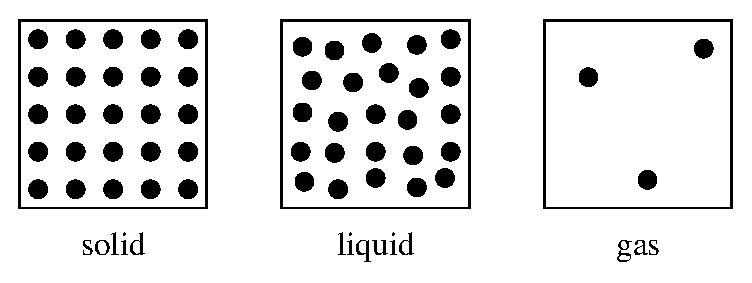
\includegraphics[width=3.5in]{liquids_and_gases/phases.eps}
\caption{The molecular picture of the phases of matter.}
\label{fig:phases}
\end{center}
\end{figure}


For most substances, there exists a boiling point separating a liquid
phase from a gas phase.  The picture you should have for the gas state
is molecules moving about freely, far from their neighbors, and moving
in a straight line until they collide with another molecule or with
the walls of the container.  Like a liquid, the gas phase is
disordered.  But the density of gases is much lower than liquids.
Another difference between liquids and gases that we can understand
immediately from the molecular viewpoint is their compressibility.
Because the gas is dilute, we can compress a gas if we push the walls
of the container inward. The molecules end up a bit closer together
and bounce around a little faster, but otherwise they don't object.
Liquids are essentially incompressible: you can't squeeze water to fit
into a smaller volume.  The liquid molecules are already packed
together, albeit in a messy way, and any further squeezing is resisted
by the repulsive forces of the pair potential.

Our basic understanding of the thermal energy of matter, developed
in sections \ref{section:thermal_kinetic_energy} and
\ref{section:thermal_potential_energy} for solids 
applies for liquids and gases as well: in particular, 
thermal kinetic energy is associated with motion of the molecules.
And the potential energy associated with
the forces between the molecules --- i.e., the pair potential ---
provides the thermal potential energy.
However, there are significant differences in the thermal
potential energy for the different phases:
\begin{itemize}
\item in the solid phase are the molecules very near their equilibrium
  separation, allowing us to approximate their forces with springs
\item in the liquid phase, however, the potential energy is
  complicated, since the molecules are pushed closer together and
  pulled farther apart as the molecules squeeze by each other, making
  the spring approximation invalid, and
\item in the gas phase, the molecules are so far apart that, except for
  very brief collisions, there is no potential energy.
\end{itemize}

In contrast to these differences, the thermal {\it kinetic energy\/}
is identical in form in all three phases.  This allows us to develop the
notion of thermal speed.

\section{Thermal Speed}

%[General use of equipartition to learn about the kinetic energy and
%  therefore the speed of the molecules, regardless of phase.  Mention
%  the displacement from eq in a solid, also.]
For all phases of matter,  the translational kinetic
energy of a single molecule is
\begin{equation}
K_\text{trans} = {\textstyle\frac{1}{2}} m v_x^2 + 
{\textstyle\frac{1}{2}} m v_y^2 + {\textstyle\frac{1}{2}} m v_z^2.
\label{eq:k_molecule}
\end{equation}
We can take advantage of this to determine how fast the molecules are
moving at some given temperature $T$.
Via the equipartition theorem, we can say that the average
translational kinetic energy is
\begin{equation}
\langle K_\text{trans}\bigr\rangle = \textstyle
  \bigl\langle\frac{1}{2}mv_x^2\bigr\rangle 
  +\bigl\langle\frac{1}{2}mv_y^2\bigr\rangle 
  +\bigl\langle\frac{1}{2}mv_z^2\bigr\rangle 
= \frac{3}{2}k_BT,   \quad\text{(single molecule)}
\end{equation}
since there are three quadratic terms in the energy.  Recalling that
$v^2=v_x^2+v_y^2+v_z^2$, we can write
\begin{equation}
%\langle K_\text{trans}\rangle = 
  \frac{3}{2}k_BT = \textstyle\bigl\langle \frac{1}{2}mv^2\bigr\rangle = 
  \frac{1}{2}m\langle v^2\rangle \quad\Rightarrow\quad
  \langle v^2\rangle = 3 k_B T/m.
\end{equation}
Now we define the thermal speed, which indicates the typical speed of
the molecules, as\footnote{Why didn't we simply define
  $v_\text{therm}$ as the average velocity $\langle \vec v\rangle$?
  Because the average velocity is zero, which tells us nothing about
  the typical magnitude of the velocity.}
\begin{equation}
  v_\text{therm} =  \sqrt{\langle v^2\rangle}= \sqrt{\frac{3k_BT}{m}} = 
  \sqrt{\frac{3RT}{M}}
\label{eq:v_thermal}
\end{equation}
where $m$ is the molecular mass and $M$ is the molar
mass.\footnote{A.k.a. what is often horribly called the ``molecular
  weight'' (horrible because its a mass, not a weight, and it's for a
  mole of molecules, not just one).  From here on, we'll abandon that
  nonsensical term and call it molar mass.} The second equality above
comes from multiplying numerator and denominator by $N_A$ and then
using $M = N_A m$ and $R=N_Ak_B$.  So we have shown, via
equipartition, a direct connection between the temperature and the
translational kinetic energy.

% Here again we have used the idea
%that temperature is related to translational kinetic energy of the
%molecules.\footnote{Again, a more general definition of temperature
%  will be provided in Chapter \ref{chapter:second_law}.}  And now we
%can say that temperature related to the speed of the molecules,
%according to Eq.~(\ref{eq:v_thermal}).

\begin{example}{Speed of Nitrogen in the Atmosphere}
What is the typical speed of a nitrogen molecule in the atmosphere at 
room temperature of $22^\circ\units{C}$?
\solution
First we need to convert the temperature to Kelvin:
%\begin{equation}
$T = 273 + 22 = 295\units{K}$.
%\end{equation}
The molar mass of elemental nitrogen is $14\units{g/mol}$.  However,
nitrogen in the air is in molecular form, $N_2$, which has two nitrogen
atoms per molecule, and a molar mass of $28\units{g/mol}$.  We
may use Eq.~(\ref{eq:v_thermal}), but to be consistent with SI units,
we should convert the molar mass to kilograms:
\begin{align}
v_\text{therm} &= \sqrt{\frac{3 R T}{M}} = \sqrt{
 \frac{3(8.31\units{J/mol$\cdot$K})(295\units{K})}{0.028\units{kg/mol}}}
\nonumber\\
&= 512\units{m/s}
\end{align}
which is the same as about 1150 m.p.h.  Room temperature molecules are fast!
\label{example:vtherm}
\end{example}

A variation of this approach (i.e., using the equipartition theorem)
can be used to determine
how much a typical molecule is displaced from its
equilibrium position but in the {\em solid phase only!}  This is discussed
(along with an example) in Sec.~\ref{sec:phase_transitions}.


\section{The Liquid State}

In the liquid state, the pair potential ``springs'' are continually
pushing and pulling and then getting stretched to the distance where
they weaken and let go.  In this way, molecules freely change their
neighbors and slide past one another, which is why a liquid can flow.
In this complicated picture, it is not possible to make a simple
calculation for the thermal potential energy.  The molar specific heat
depends in a complicated way on the details of the pair potential, and
so it varies considerably from material to material.    While physicists
and chemists have developed advanced theories for describing the
liquid state, these are beyond the scope of this course.

However, if we are given a measured specific heat, such as that of
water, we can still relate changes in the thermal energy to
temperature changes via
\begin{equation}
\Delta E_\text{therm} = n C_\text{liq}\Delta T
\end{equation}
Measured values of the specific heat are given for a few different liquids
in Table~\ref{table:liquid_specific_heats}.


\begin{table}
%\hspace{0.5in}
\begin{center}
\begin{tabular}{llc}
\hline\hline
Liquid & molecule & $C$ (J/mol$\cdot$K) \\ \hline
\noalign{\smallskip}
water & H$_2$O & 75.3 \\
methanol & CH$_3$OH & 79.5 \\
ethanol & C$_2$H$_5$OH  &  112.4 \\
acetone & (CH$_3$)$_2$CO & 125.5 \\
benzene & C$_6$H$_6$ & 134.8 \\
\hline\hline
\end{tabular}
% \caption{Molar specific heats of selected liquids.  Data is taken at 
% room temperature.}

% \begin{tabular}{llc}
% \hline\hline
% Liquid & molecule & $C$ (J/mol$\cdot$K) \\ \hline
% \noalign{\smallskip}
% water & H$_2$O & 75.3 \\
% methanol & CH$_3$OH & 79.5 \\
% ethanol & C$_2$H$_5$OH  &  112.4 \\
% acetone & (CH$_3$)$_2$CO & 125.5 \\
% benzene & C$_6$H$_6$ & 134.8 \\
% \hline\hline
% \end{tabular}
 \caption{Molar specific heats of selected liquids.  Data is taken at 
 room temperature.}
\label{table:liquid_specific_heats}
\end{center}
\end{table}

Note that $C_\text{liq}$ is different than the specific heat of the 
solid state for the same material.  It is typically larger.
For example, for copper molar specific heat in the liquid phase
is $C_\text{liq} = 36.3\units{J/mol$\cdot$K}$, compared
to $C_\text{s}=24.4\units{J/mol$\cdot$K}$ in the solid phase. 


\section{The Gas State}
\label{section:TheGasState}

In the gas phase, most of the time the molecules are so far apart that
they exert no force on each other.  The exception is the brief molecular
collision, where the pair potential plays a role in determining the forces
that they exert on each other during the collision.  However, after the
collision the pair of molecules head off in their new directions with
new speeds, moving rather quickly out of range of each other and feeling
no force.  The details of the molecular collisions are complicated,
but we can avoid having to worry about them by making use of the
equipartition theorem.

The total thermal energy for a gas is, to an excellent
approximation, purely kinetic, as the molecules are too far apart to
have an appreciable potential energy.  However, the kinetic energy 
may consist of both translational and rotational kinetic energies.
For a {\it monatomic} gas molecule, such as argon, there is no
contribution to rotational kinetic energy and so
\begin{equation}
 E_\text{molecule} = K_\text{trans} = {\textstyle\frac{1}{2}} m v_x^2 + 
{\textstyle\frac{1}{2}} m v_y^2 + {\textstyle\frac{1}{2}} m v_z^2. 
\quad\text{(monatomic ideal gas)}
\label{eq:monatomic_Emolecule}
\end{equation}
There are three quadratic contributions to the energy. 
The equipartition theorem says, therefore, that the average thermal
energy per molecule is $3(\textstyle\frac{1}{2}k_BT)$.  Therefore, the
total thermal energy is
\begin{equation}
E_\text{therm} = N\langle
E_\text{molecule}\rangle =
 {\textstyle\frac{3}{2}} N k_B T = {\textstyle\frac{3}{2}} n R T.
\quad\text{(monatomic ideal gas)}
\label{eq:monatomic_ideal_gas}
\end{equation}

\begin{figure}
\begin{center}
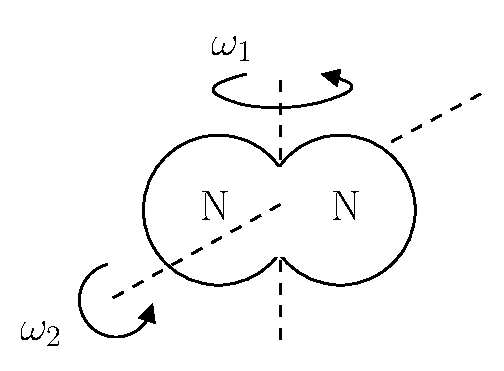
\includegraphics[width=2in]{liquids_and_gases/diatomic.eps}
\caption{Molecular nitrogen, N$_2$, has two distinct axes of rotation, 
both of which contribute to the molecular kinetic energy.}
\label{fig:diatomic}
\end{center}
\end{figure}

However, many gas molecules are diatomic, such as N$_2$, which makes up
about 78\% of our atmosphere, and O$_2$, which makes up most of the rest.
These dumbbell-shaped molecules have significant rotational kinetic energy
as well as translational kinetic energy, as shown in Fig.~\ref{fig:diatomic}.
Their molecular energy is given by
\begin{equation}
E_\text{molecule} = {\textstyle\frac{1}{2}} m v_x^2 +
{\textstyle\frac{1}{2}} m v_y^2 + {\textstyle\frac{1}{2}} m v_z^2
+{\textstyle\frac{1}{2}} I_1 \omega_1^2 + {\textstyle\frac{1}{2}} I_2
\omega_2^2
\quad\text{(diatomic ideal gas)}
\label{eq:diatomic_Emolecule}
\end{equation}
where $\omega_1$ and $\omega_2$ are the angular frequencies of the molecular
rotation about the two axes indicated in Fig.~\ref{fig:diatomic}.  The details
of the molecular mass or rotational inertia again do not matter, and 
the equipartition theorem now gives
\begin{equation}
E_\text{therm} = N\langle E_\text{molecule}\rangle
 = {\textstyle\frac{5}{2}} N k_B T = {\textstyle\frac{5}{2}} n R T.
\quad\text{(diatomic ideal gas)}
\label{eq:diatomic_ideal_gas}
\end{equation}

These results can be combined into one expression,
\begin{equation}
E_\text{therm} = \frac{f}{2} Nk_BT = \frac{f}{2} nRT.\qquad\text{(ideal gas)}
\label{eq:EthermIdealGas}
\end{equation}
where $f$ is the number of {\it degrees of freedom}, or the number of quadratic terms appearing in the energy of a molecule.  So $f=3$ for a monatomic
ideal gas, and $f=5$ for a diatomic ideal gas.

Given the usual definition of molar specific heat, $\Delta E_\text{therm}
= n C\Delta T$, we may identify
\begin{equation}
C_\text{monatomic} = {\textstyle\frac{3}{2}R} = 12.5\units{J/mol$\cdot$K}, 
\qquad
C_\text{diatomic} = {\textstyle\frac{5}{2}R} = 20.8\units{J/mol$\cdot$K}.
\end{equation}
As Table~\ref{table:gas_specific_heats} shows, these values are highly
accurate. 

\begin{table}
%\hspace{0.5in}
\begin{center}
\begin{tabular}{lcccc}
\hline\hline
Gas & Type & $C$ (J/mol$\cdot$K) \\ \hline
\noalign{\smallskip}
Neon (Ne) & monatomic & 12.5 \\
Argon (Ar) & monatomic & 12.5 \\
Hydrogen (H$_2$) & diatomic & 20.5 \\
Oxygen (O$_2$) & diatomic & 21.1 \\
Nitrogen (N$_2$) & diatomic & 20.8 \\
\hline\hline
\end{tabular}
% \caption{Molar specific heats (at constant volume) of selected gases.}


% \begin{tabular}{lcccc}
% \hline\hline
% Gas & Type & $C$ (J/mol$\cdot$K) \\ \hline
% \noalign{\smallskip}
% Neon (Ne) & monatomic & 12.5 \\
% Argon (Ar) & monatomic & 12.5 \\
% Hydrogen (H$_2$) & diatomic & 20.5 \\
% Oxygen (O$_2$) & diatomic & 21.1 \\
% Nitrogen (N$_2$) & diatomic & 20.8 \\
% \hline\hline
% \end{tabular}

\caption{Molar specific heats (at constant volume) of selected gases.}
\label{table:gas_specific_heats}
\end{center}
\end{table}

Here is an application:
Argon gas is the most abundant monatomic gas in the atmosphere, and is
technologically useful since monatomic gases conduct heat slower than
diatomic gases, due to the smaller heat capacity.  
Modern double-glazed windows have argon gas between the two
sheets of glass, to minimize the rate of heat transfer through the
window.

In solids and liquids, sound waves move by molecules pushing on their
neighbors.  In a gas, the molecules are not in contact with each other
to push and pull, and so sound propagation is fundamentally different:
the molecules must travel from collision to collision for the sound
wave to move.  Thus, the speed of the sound wave is essentially the
thermal speed of the molecules themselves, which makes for much slower
speed of sound.  While we will skip the derivation, one can show that
the speed of sound in an ideal gas is given by
\begin{equation}
v_\text{sound} = \sqrt{\frac{\gamma}{3}} v_\text{therm} = 
\sqrt{\frac{\gamma RT}{M}}.
\end{equation}
We have introduced the parameter $\gamma$, which is often called
the ``adiabatic exponent'' and is defined as 
\begin{equation}
\gamma = \frac{f+2}{f},
\end{equation}
where $f$ is again the number of degrees of freedom.
%So, for a monatomic gas, $f=3$ (see Eq.~\ref{eq:monatomic_Emolecule})
%and for a diatomic gas, $f=5$ (see Eq.~\ref{eq:diatomic_Emolecule}).  
This gives us
\begin{equation}
\gamma = \frac{5}{3} \text{\quad(monatomic), \qquad}
\gamma = \frac{7}{5}=1.4\text{\quad(diatomic).}
\end{equation}
We will see $\gamma$ again in the next lecture, since it also plays a
role in fundamental gas processes.

Notice that the speed of sound in a gas is dependent on the
temperature, since the thermal speed depends on temperature, while for
liquids and solids the speed of sound is essentially independent of 
temperature.

\begin{example}{The Speed of Sound in Air}
Estimate the speed of sound in air at room temperature of $22^\circ\units{C}
 = 295\units{K}$.  Use the average molar mass based
on an approximate composition of 78\% N$_2$ and 22\% O$_2$.
\solution
For the molar mass, we use the molar masses of nitrogen and oxygen
to find
\begin{equation}
M = 0.78 (28\units{g/mol}) + 0.22 (32\units{g/mol}) = 28.9\units{g/mol}.
\end{equation}

Both of these gases are diatomic, so we get the sound speed
\begin{align}
v_\text{sound} &= \sqrt{\frac{\gamma R T}{M}}  
=\sqrt{\frac{1.4(8.31\units{J/mol$\cdot$K})(295\units{K})}
{0.0289\units{kg/mol}}}\nonumber\\
&= 345\units{m/s}.
\end{align}
That's a pretty accurate value.  To get a more precise value we would need
to know the amount of water vapor in the air and a few other details.
\end{example}


\section{Phase Transitions}
\label{sec:phase_transitions}

Heat up an ice cube and it melts.  Heat up a chunk of copper and it
melts also, albeit at a much higher temperature.  What is melting, and
what determines the temperature at which a substance melts?  Our
ball-spring model, taken literally, cannot exhibit melting, because no
matter how energetically the molecules vibrate, they are still
connected to the same neighbors.  But we should recall that the spring
was only an approximation to the molecular pair potential, valid when
the thermal energy was low enough that the molecules were mostly near
the minimum of their potential well.  Once a pair of molecules is
stretched far enough apart, their interaction differs from a spring in
that the attractive force between them weakens and ultimately becomes
negligible (see Fig.~\ref{fig:pair_potential}).  So we need a mental
picture of a ``spring'' that weakens and ``gives up'' under too much
stretching.

We can use the ball-spring model to make a rough estimate of when
melting should occur.  The equipartition theorem tells us how far the
molecules move in their vibrations.  Let $x$ be the displacement
of a molecule from its equilibrium position in the $x$-direction.  The
average value of $x$ is zero, because the molecule is displaced equal
amounts of time in the $+x$ and $-x$ directions.  But the
average value of $x^2$ is not zero and is given by (using the
equipartition theorem)
\begin{equation}
\bigl\langle{\textstyle\frac{1}{2}}k_{sp}{x^2}\bigr\rangle =
{\textstyle\frac{1}{2}}k_{sp}\langle{x^2}\rangle 
= {\textstyle\frac{1}{2}}k_BT.
\quad\Rightarrow\quad
\langle x^2\rangle = \frac{k_BT}{k_{sp}}.
\end{equation}
This tells us the typical size of the excursions.  We can define a
thermal displacement magnitude
%\footnote{Note that we cannot use the average of
%$x$ itself to describe the size of the excursions, because $\langle x
%\rangle =0$.}
\begin{equation}
x_\text{therm} = \sqrt{\langle x^2\rangle} = \sqrt{\frac{k_BT}{k_{sp}}},
\label{eq:x_thermal}
\end{equation}
which exhibits the reasonable behavior that the higher the temperature,
the farther the molecule moves (on average) from equilibrium.  

\begin{example}{Wiggling copper atoms.}
  Copper is a solid at room temperature, $T=295\units{K}$.  As the
  copper atom oscillates about its equilibrium position, what is the
  typical magnitude of its displacement in the $x$-direction?
  \solution From Eq.~(\ref{eq:x_thermal}), we get
\begin{equation}
x_\text{therm} = \sqrt{\frac{(1.38\times 10^{-23}\units{J/K})(295\units{K})}
{29.6\units{N/m}}} =  1.17\times 10^{-11}\units{m}.
\end{equation}
where we used the copper spring constant from
chapter~\ref{chapter:thermal_energy}.  Note that we used SI
units, so $x_\text{therm}$ comes out in meters.  

Is this answer reasonable?  Recall that the equilibrium distance
between copper atoms is $d=2.28\times 10^{-10}\units{m}$, which is
about 20 times larger.  So at room temperature, copper molecules are
vibrating somewhere around 5\% of the distance of their separation.
That sounds plausible.  \end{example}

Melting occurs when the molecular excursions become an appreciable
fraction of the bond length $d$, an idea is known as the {\it
  Lindemann criterion}.  Lindemann found empirically\footnote{i.e.,
simply by looking at the experimental data} that a reasonable estimate
for the melting temperature can be obtained by setting $x_\text{therm}
\approx d/10$.  Note that if $x_\text{therm} \approx d/10$, it does
not mean that each atom in the solid is vibrating precisely $d/10$
from the equilibrium; some are going further, and some are going less.
The Lindemann criterion implies
\begin{equation}
x_\text{therm} = \sqrt{\frac{k_BT_m}{k_{sp}}} \approx d/10 \quad\Rightarrow\quad
T_m \approx \frac{d^2k_{sp}}{100 k_B}
\end{equation}
This is not an highly accurate estimate, but it does capture some
general features.  For example, lead has a relatively low melting
temperature, which is evidently due to its weak spring constant.
An estimate for copper, based on the ball-spring parameters, is
\begin{equation}
T_{m} \approx \frac{(2.28\times 10^{-10}\units{m})^2(29.6\units{N/m})}
{100(1.38\times 10^{-23}\units{J/K})} = 1120\units{K}
\end{equation}
which is comparable to the measured value of $1358\units{K}$.  Iron
has a stronger spring constant that copper, and correspondingly a 
higher melting temperature.

\begin{table}
%\hspace{0.5in}
\begin{center}
\begin{tabular}{lcccc}
\hline\hline
Material & $T_m$ (K) & $L_f$ (kJ/mol) & $T_v$ (K) & $L_v$ (kJ/mol) \\ \hline
\noalign{\smallskip}
Oxygen & 54.4 & 0.444 & 90.2 & 6.82 \\
Nitrogen & 63.2 & 0.72 & 77.4 & 5.56 \\
Ethanol & 159 & 5.02 & 352 & 38.6 \\
Water & 273 & 6.01 & 373 & 40.6  \\ 
Lead & 600 & 4.77 & 2022 & 180 \\
Copper & 1358 & 13.3 & 2835 & 300 \\
Iron  & 1811 & 13.8 & 3134 & 340 \\
\hline\hline
%\label{table:latent_heats}
\end{tabular}
% \caption{Melting and vaporization temperatures for a few materials, along
% with the latent heats of fusion and vaporization.}


% \begin{tabular}{lcccc}
% \hline\hline
% Material & $T_m$ (K) & $L_f$ (kJ/mol) & $T_v$ (K) & $L_v$ (kJ/mol) \\ \hline
% \noalign{\smallskip}
% Oxygen & 54.4 & 0.444 & 90.2 & 6.82 \\
% Nitrogen & 63.2 & 0.72 & 77.4 & 5.56 \\
% Ethanol & 159 & 5.02 & 352 & 38.6 \\
% Water & 273 & 6.01 & 373 & 40.6  \\ 
% Lead & 600 & 4.77 & 2022 & 180 \\
% Copper & 1358 & 13.3 & 2835 & 300 \\
% Iron  & 1811 & 13.8 & 3134 & 340 \\
% \hline\hline
% \label{table:latent_heats}
% \end{tabular}
%\label{table:latent_heats}
\caption{Melting and vaporization temperatures for a few materials, along
with the latent heats of fusion and vaporization.}
\label{table:phase_transitions}
\end{center}
\end{table}

In the solid state, whenever thermal energy is added to an object, the
temperature increases.  However, when the temperature of a solid
reaches the melting temperature, additional thermal energy no longer
causes temperature increase but rather phase change.  Adding a little
thermal energy to a solid at the melting temperature causes a few of
the molecules to break from the lattice structure and become liquid.
Adding more thermal energy causes even more molecules to become
liquid.  While this is happening, the temperature of the material is
not changing.  Rather, a solid with temperature $T_m$ is being
converted to a liquid at temperature $T_m$, as shown in
Fig.~\ref{fig:etherm_vs_t}.  The amount of thermal energy required to
convert one mole of a solid to a liquid is called the {\it latent heat
  of fusion}, and denoted by the symbol $L_f$.  Given the latent heat
of fusion for a material, it is straightforward to determine how much
energy is needed to melt a certain amount of that material:
\begin{equation}
|\Delta E_\text{therm}| = nL_f,\qquad\text{(melt/solidify)}
\label{eq:latent_heat}
\end{equation}
where $n$ is the number of moles of the material.  This same relation
can be used to determine how much energy is released when a certain
amount of a liquid is frozen into solid form.  Energy must be added to
melt something, and energy is released when something freezes.  Latent
heats for a few materials are given in
Table~\ref{table:phase_transitions}.

\newpage


\begin{figure}
\begin{center}
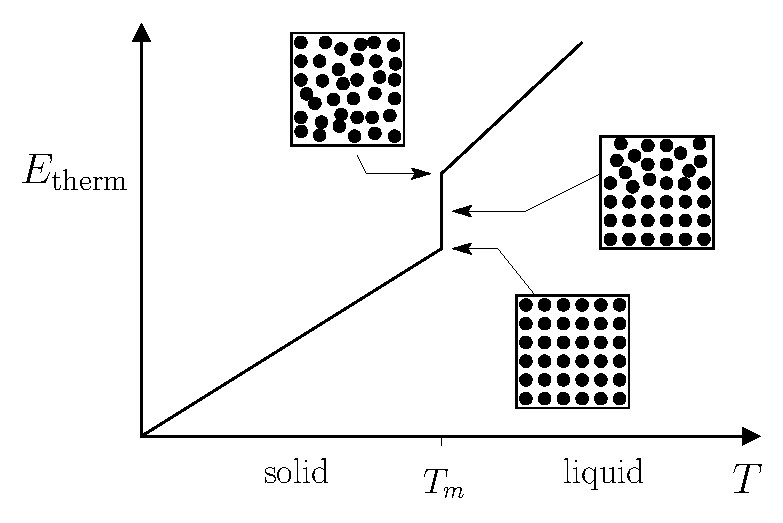
\includegraphics[width=3in]{liquids_and_gases/etherm_vs_t.eps}
\caption{Shown is $E_\text{therm}$ versus $T$ for one mole of a
  typical material.  The slopes in the solid phase and liquid phase
  are the molar specific heats, which are not typically equal to each
  other.  The vertical jump at $T_m$ represents the latent heat of
  fusion, i.e., the amount of thermal energy required to change
  phase.}
\label{fig:etherm_vs_t}
\end{center}
\end{figure}

\begin{example}{Melting lead}
  Calculate the amount of thermal energy that has to be added to 3.0 
  moles of lead at room temperature to melt $\frac{2}{3}$ of the lead. 

  \solution
  This is a two-part process.  First the temperature of the solid lead 
  solid must be raised to its melting temperature.  {\em Then} the 
  lead can be melted.

  In the first part of the process the temperature of all of the lead 
  increases to $600\units{K}$.  The thermal energy change corresponding 
  to this is given by 
  \begin{align}
    \Delta E_\text{therm}^{(1)} & = n_1C\Delta T \nonumber \\ 
    & = 3.0\units{mol}\times 26.6\units{J/mol$\cdot$K} \times
        (600\units{K} - 295\units{K}) \nonumber \\
    & = 24.3 \units{kJ}
  \end{align}
  In the second part of the process the phase changes, so the 
  thermal energy change necessary to melt two moles of the lead is given by
  \begin{align}
    \Delta E_\text{therm}^{(2)} & = n_2 L_f \nonumber \\ 
    & = 2.0\units{mol} \times 4.77\times 10^3\units{J/mol} \nonumber \\
    & = 9.5\units{kJ}
  \end{align}
  Combining these two thermal energy changes gives
  \begin{align}
    \left(\Delta E_\text{therm}\right)_\text{total} 
    & = \Delta E_\text{therm}^{(1)} + \Delta E_\text{therm}^{(2)} \nonumber \\
    & = 24.3\units{kJ} + 9.5\units{kJ} \nonumber \\
    & = 33.8\units{kJ} \
  \end{align} 
  In this calculation, we used the measured value for the molar
  specific heat for lead (see Table \ref{table:material_properties}).
  We could have used the Dulong-Petit (ball-spring) approximation ($C
  = 3R$) which would have given us a result very close to the value
  that we calculated here.

  Note also that if we wanted to start with 2 moles of liquid lead 
  and 1 mole of solid lead both at $600\units{K}$, and cool it down to 
  a solid at room temperature, the same calculation would
  tell us how much thermal energy we would need to {\em remove}.  It
  would also be $33.8\units{kJ}$.
\end{example}


%We can make an estimate for the magnitude of the latent heat.  The
%melting temperature was determined by the energy $k_BT_m$ required to
%stretch the molecular bond by an amount $d/10$.  In the liquid state
%the molecules are not so neatly arranged as in the solid state, so the
%bonds are even farther stretched. The energy required for this
%additional stretching is the latent heat of fusion, which should be an
%energy comparable to $k_BT_m$.  It turns out that
%\begin{equation}
%  L_f \approx N_A k_B T_m = R T_m
%\end{equation}
%is a decent rough estimate for the latent heat of fusion for one mole
%of material.
%
%Interestingly, we can use the same latent heat whether we are adding
%thermal energy to  a solid to melt it, or removing thermal energy from
%a liquid to solidify it.  The latent heat merely reflects the
%potential energy difference of the solid versus liquid configuration
%of molecules.

For most substances, there exists a boiling point separating a liquid
phase from a gas phase.  At the molecular level, the liquid state has
nearly solid-like density, with molecules packed close together and
fairly near the minimum of the potential well.  The transition to the
gas phase requires pulling these molecules apart and setting them
free, where they have no neighbors.  Let $E_\text{bind}$ be the depth
of the potential well, that is, $E_\text{bind}$ is the amount of
energy needed to bring a pair of molecules from their equilibrium
separation to far apart from each other (see
Fig.~\ref{fig:boiling}(a)).  Vaporization (or boiling) occurs roughly
when $k_BT\approx E_\text{bind}$, so we can estimate the boiling
temperature as
\begin{equation}
  T_v\approx\frac{E_\text{bind}}{k_B}.
\label{eq:t_v}
\end{equation}

\begin{example}{Molecular Binding Energy}
  Estimate the molecular pair binding energy $E_\text{bind}$ for
  copper, using the information in
  Table~\ref{table:phase_transitions}.  \solution Copper vaporizes at
  $T_v = 2835\units{K}$, so we may estimate
  \begin{equation}
    E_\text{bind}^{\rm Cu} \approx k_B T_v = (1.38\times 10^{-23}\units{J/K})
    (2835\units{K}) = 3.91\times 10^{-20}\units{J}.
  \end{equation}
  A convenient energy unit for describing molecular bonds is the
  electron volt (eV), defined as
  \begin{equation}
    1\units{eV} = 1.60\times 10^{-19}\units{J}.
  \end{equation}
  In terms of electron volts, then,
  \begin{equation}
    E_\text{bind}^{\rm Cu} = 
    \frac{3.91\times 10^{-20}\units{J}}{1.60\times 10^{-19}\units{J/eV}} 
    = 0.245\units{eV}
  \end{equation}
\end{example}

\begin{figure}
\begin{center}
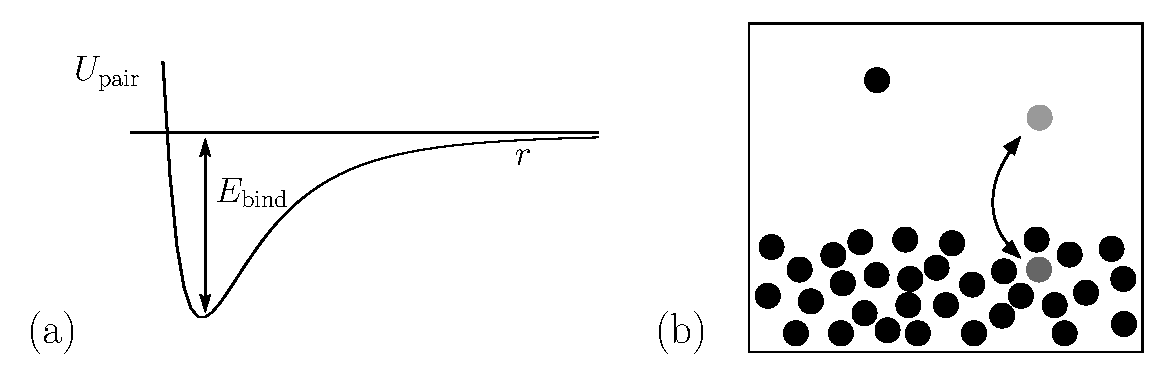
\includegraphics[width=4.4in]{liquids_and_gases/boiling.eps}
\caption{(a) The pair potential depth $E_\text{bind}$.  (b) Removing a particle
from the liquid state requires an energy of about 10--12$E_\text{bind}$.}
\label{fig:boiling} 
\end{center}
\end{figure}

Like with melting, vaporization requires an input of thermal energy.
As thermal energy is added, the temperature remains fixed at the
vaporization temperature, while an increasing amount of liquid gets
converted to gas.  The amount of energy required to convert a mole of
a substance from liquid to gas is called the {\it latent heat of
  vaporization}.  This is used much the same way as the latent heat of
fusion:
\begin{equation}
  |\Delta E_\text{therm}| = nL_v. \qquad\text{(vaporize/condense)}
\end{equation}
As before, $\Delta E_\text{therm}$ is positive if we are adding
thermal energy to vaporize, and it is negative if we are removing
thermal energy to condense.

%We can estimate this energy by realizing that a
%sphere in three dimensions surrounded by spheres of the same size has
%typically 10--12 neighbors.  This is illustrated in
%Fig.~\ref{fig:boiling}(b), though the number of neighbors appears
%smaller because it is a two-dimensional drawing.  Evidently it is
%necessary to add an energy of about $12E_\text{bind}$ to convert a molecule
%from the liquid state to the gas state.\footnote{This estimate takes
%  into account the additional energy required to make space for the
%  new gas molecule.}  We can relate this to the vaporization temperature
%via Eq.~\ref{eq:t_v} and get a ``rule of thumb'' for the latent
%heat of vaporization
%\begin{equation}
%L_v \approx N_A(12E_\text{bind}) \approx 12 N_A k_BT_v  = 12RT_v.
%\end{equation}
%Compared to the latent heat of fusion,
%we see that this latent heat is rather large!  The thermal energy of
%copper from solid to liquid to gas is shown in
%Fig.~\ref{fig:copper_etherm}.  Note that the same latent heat applies
%whether boiling a liquid or condensing a gas: in the former case the
%thermal energy is being added, while in the latter case it is being
%removed.
%
%\begin{figure}
%\begin{center}
%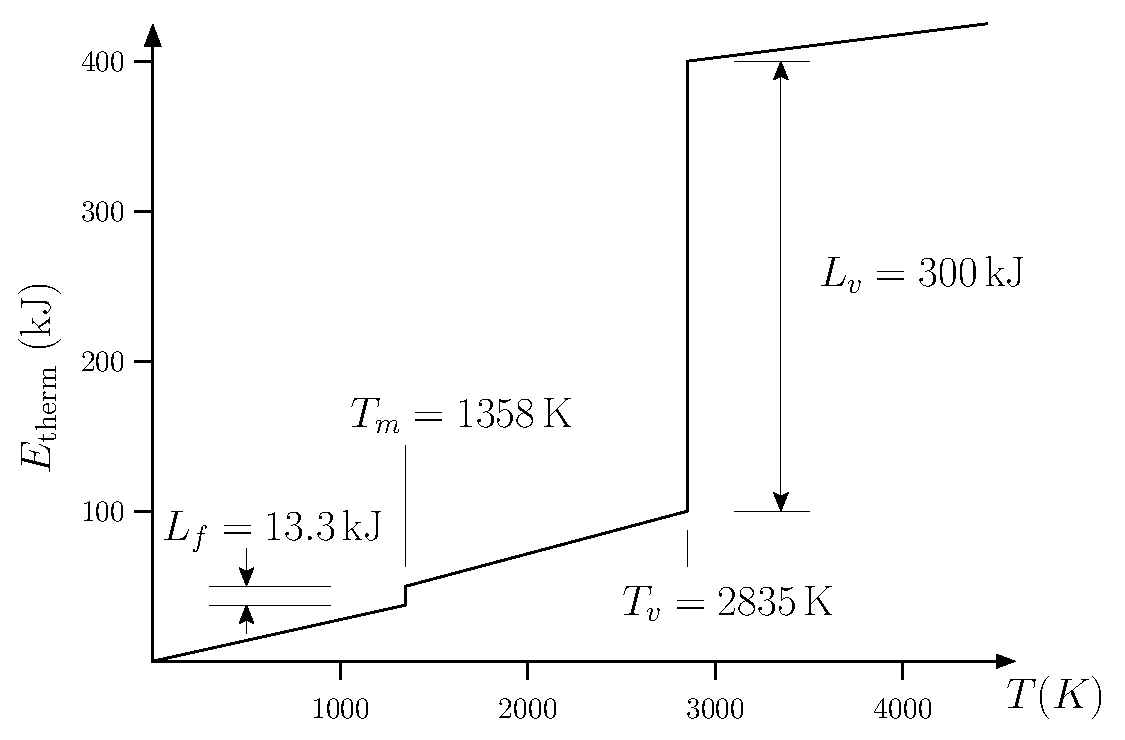
\includegraphics[width=4in]{liquids_and_gases/copper_etherm.eps}
%\caption{$E_\text{therm}$ versus $T$ for one mole of copper as it goes
%  from solid to liquid to gas.  The latent heat of vaporization is
%  large!  Within the phases, the slope indicates the molar specific
%for that phase.}
%\label{fig:copper_etherm}
%\end{center}
%\end{figure}

One final comment about latent heat and phase transitions: the amount
of heat needed to melt or boil most common materials is quite large.
Just looking at Tables \ref{table:material_properties} and
\ref{table:phase_transitions}, you can see that it is necessary to add a
``k'' to the units for latent heats $L_f$ and $L_v$ (versus the units
for molar specific heat $C$) because we are usually talking about
thousands of Joules of energy to cause a phase transition for each
mole of the substance.  This is a very important result with {\it
  lots} of practical applications.  For example, this is the reason
why ice is so good at cooling your drink; it isn't the low {\em
  temperature} of the ice that is important, rather it is the large
amount of energy that the ice absorbs when it melts that does such a
good job of cooling your drink.  Phase transitions are used {\em all
  the time} in cooling and heating applications.  A standard air
conditioner or refrigerator typically uses some substance (e.g.,
freon) whose condensation and vaporization play a key role in the
cooling process.  And your body uses phase transitions to keep cool on
hot summer days.  Sweat (water) on your skin vaporizes, and most of
the energy needed for this phase transition comes from your body.
This is how you can manage not to overheat even if the surrounding air
temperature is greater than your body temperature.  So, we would all
be dead were it not for phase transitions.

\section{Pressure}

Liquids and gases push outwardly on their surroundings.  To describe
this push we introduce the concept of {\it pressure}.  Consider a
liquid or a gas enclosed in some container, and focus on one wall of
the container with area $A$, such as shown in
Fig.~\ref{fig:gas_pressure}.  The fluid pushes on the wall in the
perpendicular direction with a force of magnitude $F$.  Pressure is
then the force per area
\begin{equation}
  p=\frac{F}{A},
\end{equation}
and has units N/m$^2$.  This combination of units is given the name
pascal (Pa), that is, $1\units{Pa} = 1\units{N/m$^2$}$.  Atmospheric
pressure is given by
\begin{equation}
  p_\text{atm} = 1.01\times 10^{5} \units{Pa} = 101\units{kPa}.
\end{equation}
Note that pressure applies to more than just liquids and gases.  Any
time that there is a force exerted on a surface, you can define a
pressure simply by dividing that force by the surface area.
Conceptually, the pressure indicates how ``spread out'' the force is,
i.e., if the same force is exerted over a larger surface area, then
there is less force per unit area (smaller pressure) and each part of
the surface experiences a smaller force.  That is why, for example, it
is useful to wear snowshoes with a large surface area when walking
over fresh snow --- the downward force you exert on the ground is
spread over a larger area, resulting in a smaller pressure on the
snow, so the snow doesn't collapse.

Pressure does not have a direction.  If we consider some point in the
fluid, pressure is an outward push in all directions.  This outward
push is balanced by an identical outward push from a neighboring
region of the gas.  Only at the boundaries of the gas is there an
imbalance --- here the enclosed gas is only pushing from inside --- and
that is where we can measure the pressure.  And note:  {\bf a gas
can ONLY push on a surface; it NEVER pulls!!!}

\begin{figure}
\begin{center}
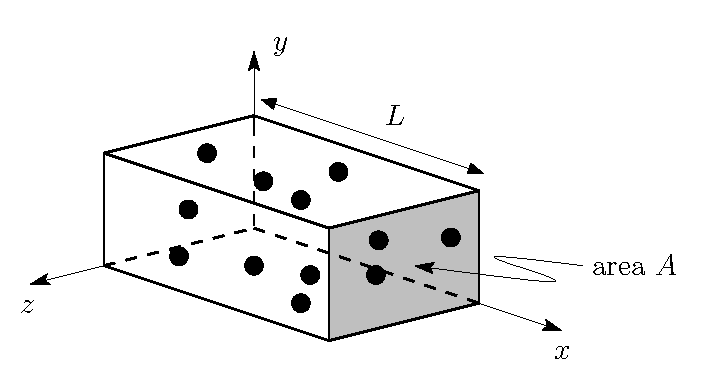
\includegraphics[width=3.5in]{liquids_and_gases/gas_pressure.eps}
\caption{A gas enclosed in a container of length $L$, with the shaded
wall having area $A$.}
\label{fig:gas_pressure}
\end{center}
\end{figure}

We can use our picture of the gas state to derive the pressure of a
gas.  In the {\it ideal gas} approximation we ignore collisions
between the molecules entirely, and treat each molecule as bouncing
back and forth between the walls of the container.  The particles bouncing
off the walls exert a force on the wall, and this is precisely the 
origin of pressure.

\newpage

\begin{example}{Pressure and Balloons}
  Explain qualitatively how the gas inside an inflated balloon
  prevents the balloon from collapsing.

  \solution When a balloon is inflated, the rubber is stretched in all
  directions, resulting in an increased tension.  At every point along
  the surface of the balloon fabric, the tension pulls in all
  directions along the surface.  Because of the curvature of the
  balloon, these tension forces add up to give a net inward tension
  force.

  The inward components of the tension do not cause the balloon to
  collapse because there is an outward force due to air molecules
  trapped within the balloon bouncing off the inner surface of the
  balloon.  Each time a molecule bounces off a piece of the balloon,
  it gives that piece a small outward kick.  Of course, there are also
  molecules outside the balloon, and each time one of these bounces
  off the balloon, it gives a small inward kick.  If the outward and
  inward forces were balanced, which is what happens with an open
  balloon, then the net force would be the tension force, and the
  balloon would rapidly shrink.

  But what if the collisions from the inside molecules are more
  frequent and/or harder collisions?  Consider that there are
  around $10^{23}$ gas molecules in a typical balloon, and they are
  moving quite fast at typical room temperatures (see Example
  \ref{example:vtherm}).  There are a {\bf lot} of collisions occurring
  each second between gas molecules and the inside of the balloon.
  The result of all of these collisions is an outward force exerted on
  the balloon fabric by the gas molecules.  This outward gas force
  opposes the inward components of the tension {\it and} the inward
  force due to the collisions of all the gas molecules on the outside,
  and as a result the balloon does not collapse.
\end{example}

\section{The Ideal Gas Law}

Now that we know how it is that a gas can exert a pressure, we
can use these ideas --- along with the previous discussion of
thermal velocities of gas molecules --- to calculate how the
pressure relates to the temperature of the gas, the number of gas
molecules (or moles) and the geometry of the container holding the
gas.  From this we will derive one of the most useful 
relations in thermodynamics: the {\em ideal gas law}.

 A collision with a wall is shown in Fig.~\ref{fig:collide_wall}.
 Note that the $x$-component of velocity changed sign, while the
 $y$-component of the velocity was unchanged.  If we focus on $v_x$,
 we can see that the molecules in Fig.~\ref{fig:gas_pressure} will
 bounce off the shaded wall and change the sign of $v_x$, then a time
 $L/v_x$ later they will bounce off the back wall and head back toward
 the shaded wall.  They will likely bounce off the side walls en
 route, but this has no effect on $v_x$, so we can ignore it.  Thus
 the time between collisions on the shaded wall is $\Delta t = 2L/v_x$
 (the factor of two coming from the trip away and then back).


The force on the wall due to the particle is zero in between
collisions, and then very abruptly some non-zero value during the
collision.  Viewed as a function of time, the force would be a series
of spikes, since each collision is short in duration, and then there
is no force while the particle travels to the other side of the
container and back again. What we feel as steady pressure is the time
average of many collisions, so we would like to obtain an average of
this force over time.  


\begin{figure}
\begin{center}
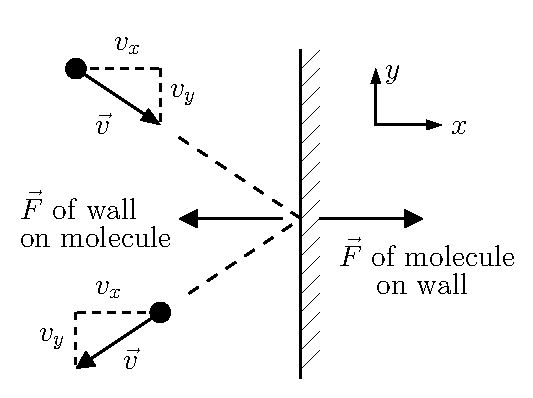
\includegraphics[width=2.6in]{liquids_and_gases/collide_wall.eps}
\caption{The $x$-component of velocity changes sign, while the $y$-component
of velocity is unchanged.}
\label{fig:collide_wall}
\end{center}
\end{figure}

We can calculate this time averaged force first by noting that the force
of the molecule on the wall is, by Newton's third law, equal and opposite
the force of the wall on the molecule.  The force of the wall on the molecule
causes a change in the $x$-component of momentum, $p_x$ (see 
Fig.~\ref{fig:collide_wall}).  Note that the symbol $p$ here, and in the 
next two equations,  refers to momentum, not pressure. We apologize for 
the fact that the standard symbols for these quantities are the same
(but there are only so many letters to use).  The momentum change is 
given by 
\begin{equation}
\Delta  p_x  = - mv_x - m v_x = -2mv_x.
\end{equation}
This momentum change happens once every time interval of $\Delta t =
2L/v_x$ (the travel time between collisions), so we can conclude the
average force of the wall on the molecule is
\begin{equation}
F_{{\rm avg},x} = m a_\text{avg}= \frac{m \Delta v_x}{\Delta t} =\frac{\Delta p_x}{\Delta t} = -\frac{2mv_x}{2L/v_x} =
-\frac{mv_x^2}{L}.
\end{equation}
The average force of the {\it molecule on the wall} is then
equal and opposite.  If we consider all $N$ molecules, then we can
conclude
\begin{equation}
F_{\text{on wall},x} = \sum_i \frac{m v_{i,x}^2}{L}
\end{equation}
where $v_{i,x}$ is the $x$-component of the velocity $\vec v_i$ of the
$i$th particle.
We can appeal to the equipartition theorem, which tells us
\begin{equation}
\Bigl\langle\sum_i {\textstyle\frac{1}{2}} m v_x^2\Bigr\rangle = N
\bigl({\textstyle\frac{1}{2}}k_BT\bigr),
\end{equation}
and so the average force on the wall is given by
\begin{equation}
F_{\text{on wall},x} = \frac{Nk_BT}{L}.
\end{equation}
Finally, we use the definition of pressure to conclude
\begin{equation}
p = \frac{F_{\text{on wall},x}}{A} = \frac{Nk_BT}{AL} = \frac{Nk_BT}{V}
\end{equation}
where we have used $V=AL$ (see Fig.~\ref{fig:gas_pressure}).  This
last relation holds regardless of the shape of the container, and we
have thus derived the {\it ideal gas law}
\begin{equation}
pV = N k_BT \qquad \text{or}\qquad pV = nRT.
\label{eq:ideal_gas_law}
\end{equation}
This is another universal law where the details of the molecules are
irrelevant: the molecular mass canceled out, and any interaction
forces between the molecules negligible as long as the gas is dilute
enough.

This is an extremely accurate law for most gases at room temperature and
higher temperatures.  Note also that it does not depend on the mass of
the gas molecule, or whether it is diatomic or monatomic.

In Eq.~(\ref{eq:ideal_gas_law}), both sides of the equations have units
of energy.  If we use SI units, pressure should be measured in pascal,
and volume should be measured in cubic meters.   However, we may take
advantage of the relation
\begin{equation}
1\units{J} = (1\units{Pa})(1\units{m$^3$}) = 
(10^{-3}\units{kPa})(10^3\units{L}) = (1\units{kPa})(1\units{L}),
\end{equation}
where $L$ is liters.  This tells us we can use kilopascals and liters and
the product $pV$ will turn out to be joules.  

\begin{example}{Volume of a Mole of Gas}
  Calculate the volume in liters occupied by a mole of ideal gas at a
  temperature of $22^\circ\units{C}$ and atmospheric pressure.

  \solution Starting from Eq.~(\ref{eq:ideal_gas_law}), we solve for
  $V$:
  \begin{equation}
    V = \frac{nRT}{p} = \frac{(1\units{mol})(8.31\units{J/mol$\cdot$K})
      (295\units{K})}{101\units{kPa}} = 24.2\units{L}.
  \end{equation} 
  Note that we had to convert temperature from Celsius to Kelvin in
  this calculation.  {\bf This is important:} you {\bf always} have to
  use Kelvin for the temperature when using the ideal gas law.
\end{example}

\begin{exampleb}{Using Ratios in the Ideal Gas Law}
  An ideal gas at a temperature $50^{\circ}$ C is in a car piston.
  The piston compresses the gas to 1/3 of its original volume.  The
  pressure increases by a factor of 5 during this process.  Calculate
  the new temperature of the gas in the piston.

  \solution We don't know the volume, pressure or number of moles of
  gas at any point in this problem, so we will have to solve this
  problem using ratios.

  First, we need to convert temperature to Kelvin: $T = (50+273)
  \units{K} = 323 \units{K}$.  Next, write down the ideal gas law: $pV
  = nRT$.  We are interested ultimately in the final temperature, so
  re-write this as:
  \begin{equation}
    T = \frac{pV}{nR}
  \end{equation}
  This holds both initially and after the compression, so $T_1 =
  p_1V_1/(n_1R)$ and $T_2 = p_2V_2/(n_2R)$.  
\begin{equation}
  \frac{T_2}{T_1} = \frac{\displaystyle\left(\frac{p_2V_2}{n_2R}\right) }
 {\displaystyle\left( \frac{p_1V_1}{n_1R}\right) } 
  = \frac{p_2}{p_1}\frac{V_2}{V_1},
\end{equation}
since $n_2 = n_1$ and $R$ is a constant.  So, the final temperature is
\begin{equation}
  T_2 = T_1 \cdot \frac{p_2}{p_1}\cdot\frac{V_2}{V_1} = 
  (323\units{K})\cdot 5 \cdot \frac{1}{3}
  = 538 \units{K} ,
\end{equation}
or $(538 - 273)^{\circ}\units{C} = 265^{\circ}\units{C}$.

Note that when using ratios to determine a new value for the pressure
or volume, it doesn't matter what units we use for those quantities
because the units will cancel between numerator and denominator. 
%For example, if the initial volume is in cm$^3$, then the final volume
%will be in cm$^3$.
Though it is still always necessary to use Kelvin for temperature.
\end{exampleb}

\newpage

\section*{Problems}
\markright{PROBLEMS}

%[Assigned: A46 - sucking tubes. A47 - dunking birds.]

\begin{problem} {\bf Melting iron}
  \begin{enumerate}
  \item Use your results from
    Problem~\ref{chapter:thermal_energy}.\ref{problem:ball-spring_iron}
    to estimate the typical thermal displacement for atoms in a chunk
    of solid iron at room temperature.  (Assume a room temperature of
    $22^{\circ}\units{C}$.)  Compare your result to the typical
    lattice separation for the iron atoms.  Based on this result and
    the Lindemann criterion, explain why it is reasonable that iron is
    a solid at room temperature.

  \item Now, assuming that iron melts when the typical displacement is
    one-tenth the lattice separation (i.e., $x_\text{therm} \approx
    d/10$, which is the Lindemann criterion), estimate the melting
    temperature of iron.  Compare your result to the experimental
    value.

  \item Write a sentence explaining in your own words why the melting
    temperature should be related to the typical thermal displacement
    $x_\text{therm}$.  Don't worry so much about the factor $1/10$ in
    the Lindemann melting criterion, but your explanation {\bf should}
    state why melting occurs when $x_\text{therm}$ gets sufficiently large.
  \end{enumerate}
\label{problem:iron_melting}
\end{problem}

%\begin{problem}  % maybe replace with something more useful!
%  Of the substances listed in Table~\ref{table:phase_transitions}, one
%  deviates significantly (more than a factor of two) from the estimate
%  that the latent heat of fusion is roughly $k_BT_m$ per molecule.
%  Identify the substance.  Can you make a guess why?
%\label{problem:sesame_street}
%\end{problem}

\begin{problem}
Calculate the thermal speed at temperature $22^\circ\units{C}$ of
\begin{enumerate}
\item molecular oxygen (O$_2$)
\item methane (CH$_4$)
\item carbon dioxide (CO$_2$)
\end{enumerate}
\label{problem:thermal_speeds}
\end{problem}

\begin{problem}
A 100\units{g} piece of ice at $0^\circ\units{C}$ is placed into a
container holding 200\units{g} of water, initially at temperature
$25^\circ\units{C}$.  Heat flows from the water to the ice, cooling the water
and melting the ice. 
% The specific heat of water is
%$C=75.3\units{J/mol$\cdot$K}$.
\begin{enumerate}
\item Calculate how many moles of ice and how many moles of water are
initially present.
\item  Determine how much 
heat flows out of the water in cooling to  $0^\circ\units{C}$.
\item Determine how many moles of ice are melted by this added heat.
\end{enumerate}
\label{problem:water_calorimetry}
\end{problem}

\begin{problem}
Compare two containers of the same ideal gas; each container has 
the same volume and the same number of molecules.  The temperature 
of the gas in the first container is twice the temperature in the 
second container,
$T_1=2T_2$.  Find the following ratios
\begin{enumerate}
\item $v_\text{therm,1}/v_\text{therm,2}$.
\item $K_\text{molec,1}/K_\text{molec,2}$.
\item $p_1/p_2$.
\end{enumerate}
\label{problem:ideal_gas_ratios}
\end{problem}

\begin{problem}
How many moles are in 3 liters of ideal gas at pressure $200\units{kPa}$
and temperature $100^\circ\units{C}$?
\label{problem:ideal_gas_moles}
\end{problem}

\begin{problem} 
  Using the vaporization temperature of water to estimate the pair
  binding energy for water molecules.
%\begin{enumerate} 
%\item Calculate the ratio $L_v/k_BT_v$ for each substance in
%  Table~\ref{table:phase_transitions}.  Compare your results with the
%  ``rule of thumb'' presented in section~\ref{section:boiling}.
%\item Estimate the pair binding energy for water molecules.
%\end{enumerate}
\label{problem:heat_of_vaporization}
\end{problem}


\begin{problem}
Calculate the speed of sound in a gas of pure molecular hydrogen at a
temperature of $22^\circ\units{C}$.
\label{problem:speed_of_sound}
\end{problem}


% handins begin

%[Handins begin here.  A48 - blow dart suction]


\begin{problem}
One mole of water at $20^\circ\units{C}$ has 20\units{kJ} of thermal
energy added.  Calculate the number of moles which remain in the liquid
state.
\end{problem}


\begin{problem}
Rank the following according to the speed of the molecules at room
temperature, from fastest to slowest:
\begin{enumerate}
\item copper (solid)
\item water (liquid)
\item krypton (gas)
\item molecular nitrogen (gas)
\end{enumerate}
\end{problem}


\begin{problem}
A fixed amount of ideal gas is at temperature $25^\circ\units{C}$,
volume $4.0\units{L}$ and pressure $100\units{kPa}$.  The temperature
of the gas is increased to $80^\circ\units{C}$ while the volume is
decreased to $3.2\units{L}$.  Determine the new pressure.
\end{problem}

\begin{problem}
  For silver, the ball-spring parameters are $m=1.79\times
  10^{-25}\units{kg}$, $d=2.58\times 10^{-10}\units{m}$, and
  $k_{sp}=21.4\units{N/m}$.  Based on this information, estimate the
  melting temperature and latent heat of fusion for silver.  
\end{problem}

% Problems using Schroeder's molecular dynamics applet - very rough drafts

%\begin{problem}
%{\bf Solid-liquid coexistence.}  For this problem you will use the
%molecular simulation applet available online.  
%(A link to the simulations
%can be found on today's Calendar page for today's lecture.)
%Load in the preset [preset will specify the number of particles, 
%a little bit of gravity, and a thermal energy that results 
%in a busy liquid phase].  Vary the thermal energy until you 
%find a value gives you
%liquid-solid coexistence.  Determine the thermal energy values
%corresponding to
%\begin{enumerate}
%\item when the system has just left the liquid-solid coexistence and
%  completely solidified.
%\item when the system has just left the liquid-solid coexistence and
%  completely melted.
%\item How would expect the molecular kinetic energies to compare at
%  these two points?  [they woudl be essentially equal, since the
%    temperature hasn't been changing, only the phase]
%\end{enumerate}
%\end{problem}

%  500 atoms, atom size=10, gravity=0.1, timestep =0.004, animation speed=50
% works well for a liquid.

%\begin{problem}
%{\bf Diatomic versus monatomic gases.} For this problem you will use
%the molecular simulation applet available online. 
%(A link to the simulations can be found on today's 
%Calendar page for today's lecture.) In
%fact, you will need to open two browsers and start up two separate
%simulations.  In the first simulation, load the monatomic ideal
%gas preset.  In the second simulation, load the diatomic gas preset.
%You also might want to reduce the animation speed so that the motion
%is easy to follow (on faster computers, an animation speed of 10 is
%sometimes good).
%\begin{enumerate}
%\item Assign the same value of thermal energy to each system.  (You
%  might want to click ``Slower'' a few times to get to manageable
%  speeds.  For reference, a thermal energy of around 80 works well).  Note
%  that they have the same number of particles, so the average energy
%  per particle should be equal in the two cases.  How does it look?
%  Are they moving at comparable speeds?
%\item No, they aren't.  Now increase the thermal energy of the system
%  that looks to be moving slower until, roughly by eye the molecules
%  in the two systems appear to be moving at comparable speeds.  Record
%  your $E_\text{therm}$ values for the diatomic and monatomic gases.
%\item What's going on here?  (Hint:  for a monatomic gas, the energy
%  all goes into translation of the atoms.  For a diatomic molecule,
%  where does the energy go to?)  Can you explain your answer to (a)?  Your
%  explanation should lead to a prediction for the ratio of the
%  $E_\text{therm}$ values.  What is the prediction, and how do your
%  values compare?  
%\end{enumerate}
%\end{problem}

\begin{problem} {\bf Let's play microwave.}  This is just fun, and
  you've got to do it.  Load up the molecular dynamics applet, select
  the solid preset, and click ``Start''.  Now we're going to melt the
  solid without adding heat.  This is exactly what a microwave oven
  does: the microwaves do work, pushing and pulling molecules around,
  and this gets converted to thermal energy.  So let's do the same
  thing.  You can ``pull'' a molecule by clicking on it and dragging
  it.  Reach in and pull on a molecule, and then wait and watch how the
  system responds.  Now do it again.  Keep doing it until you've fully
  melted the solid.  (Notes: it might help to reduce the ``Animation
  speed'' so that you can see what is going on.  You also might have
  to pull your mouse a large distance quickly before letting go when
  ``pulling'' a molecule.)

\begin{enumerate}
\item Describe what you observe in the simulation and what you had to
  do to melt the solid by pulling on individual atoms.  {\bf
    Question:} Why would pulling on just one or two individual atoms
  melt the entire solid?

\item Now think of something else cool to do with the applet.  Write a
  few sentences describing what you did and what you found.
\end{enumerate}
\end{problem}

\begin{problem}
  Aquaman buys a balloon filled with a fixed amount of helium from a
  street vendor in New York City on a hot $37^{\circ}\units{C}$ day.
  He measures the pressure inside the balloon to be $1.1\units{atm}$
  ($1\units{atm}=101\units{kPa}$).  When he arrives at the underwater
  city of Atlantis, he discovers that the balloon is now 0.40 times
  the original volume.  His thermometer indicates that the ocean has a
  temperature of $2^{\circ}\units{C}$.  Determine the pressure inside
  the balloon.
\label{problem:aquaman}
\end{problem}

\begin{problem}
  Let's consider the ideal gas law $pV = nRT$ qualitatively from a
  perspective of molecules of the gas hitting the shaded side of a
  container, as shown in Fig.~\ref{fig:ideal_gas_problem}.
  \begin{figure}[ht]
    \begin{center}
      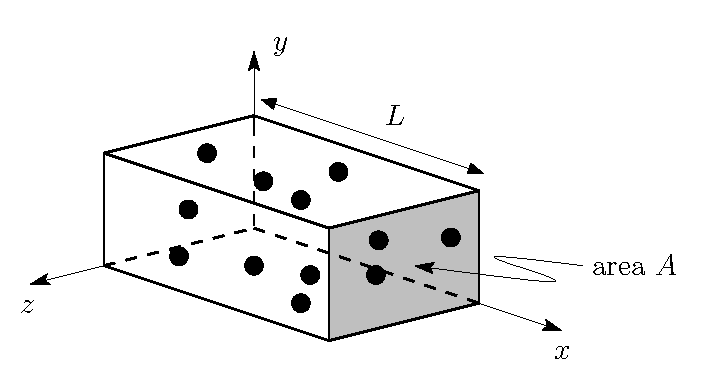
\includegraphics[width=3.5in]{liquids_and_gases/gas_pressure.eps}
      \caption{For problem~\ref{problem:ideal_gas_law}.  Gas in a
        container of length $L$ and cross section $A$.}
      \label{fig:ideal_gas_problem}
    \end{center}
  \end{figure}
  \begin{enumerate}
  \item Considering collisions of gas molecules with the wall, explain
    qualitatively why the pressure of a gas increases if the
    temperature of the gas increases, with everything else constant.
    There are two different reasons why increasing the temperature
    increases the pressure.
  \item Explain qualitatively why the pressure of a gas increases if
    the number of moles of gas molecules in the gas increases, with
    everything else constant.
  \item Explain qualitatively why the pressure increases if the volume
    of the container holding the gas decreases, with everything else
    constant.  There are actually two different reasons why decreasing
    the volume increases the pressure: one is a result of decreasing
    $L$ and the other is a result of decreasing $A$.
  \end{enumerate}
  \label{problem:ideal_gas_law}
\end{problem}
\newpage

\begin{problem}
  In this problem you will make some simplifying assumptions and estimate 
  the pressure of a gas of nitrogen molecules from a microscopic picture 
  of the gas.  Assume that the gas is in a $10\units{cm} \times 
  10\units{cm}\times 10\units{cm}$ box at room temperature, 
  $T = 22^\circ\units{C}$.  The assumptions are:
  \begin{itemize}
  \item All the molecules travel at the speed $v_\text{therm}$ derived 
  in Example~\ref{example:vtherm}.  This is 
  not actually true --- there is a spread in 
  molecular speeds around the average ---
  but $v_\text{therm}$ is a typical speed.
  \item One third of the molecules in the gas travel in the $\pm x$-direction,
  one third travel in the $\pm y$-direction, and one third travel in the 
  $\pm z$-direction.  This is obviously not true, but this assumption will
  simplify the calculations.
  \end{itemize}
 
  \begin{figure}[ht]
    \begin{center}
      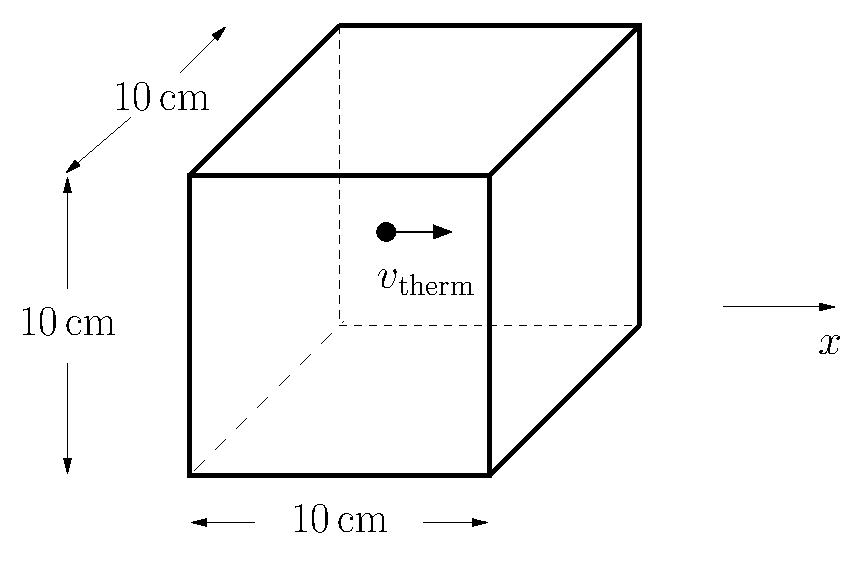
\includegraphics[width=2.5in]{liquids_and_gases/ideal_gas_prob.eps}
      \caption{Figure for problem~\ref{problem:ideal_gas_quant}.}  
      \label{fig:ideal_gas_quant}
    \end{center}
  \end{figure}
  
  \begin{enumerate}
  \item Calculate the numerical value of the {\em change} in the momentum of 
  a single nitrogen molecule traveling in the $x$-direction after it 
  collides elastically with the right wall of the container.  (If you 
  need help determining the speed of the nitrogen molecules, see Example
  \ref{example:vtherm}.)
  \item Calculate the number of times this single nitrogen molecule 
  collides with the right wall of the container in 1 second.
  \item Calculate the total change in momentum of the molecule in 1 second
  due to collisions with the right wall of the container.
  \item Calculate the average force on the right wall of the container 
  due to collisions with the single molecule.
  \item At room temperature and atmospheric pressure, the number density, 
  (i.e., the number of molecules per unit volume) of 
  nitrogen molecules is $2.49\times 10^{19}\units{molecules/cm$^{3}$}$.  
  Use the second of our simplifying assumptions and calculate the 
  average force on the right wall of the container due to all of the 
  molecules in the gas. 
  \item Calculate the pressure that the gas exerts on the right wall
  of the container.  Compare your answer to atmospheric pressure 
  ($1\units{atm} = 1.01\times 10^5\units{Pa}$). 
  \end{enumerate}
  \label{problem:ideal_gas_quant}
\end{problem}


%\chapter{Gas Processes}
\label{chapter:gas_processes}

This chapter will be distributed separately, some time in October or
November.

% \section{Introduction}

% \newpage

%\section*{Problems}
%\markright{PROBLEMS}

%\begin{problem} 
% Three identical gas-cylinder systems are compressed from the
% same initial state to final states that have the same volume, one
% isothermally, one adiabatically, and one isobarically. Which
% system has the most work done on it? The least?
%\label{prob:}
%\end{problem}

%\begin{problem}
% By what factor must the volume of a gas with $\gamma = 1.4$ be
% changed in an adiabatic process if the kelvin temperature is to
% double?
%\label{prob:}
%\end{problem}

%\begin{problem}
% By how much does the temperature of (a) an ideal monatomic
% gas and (b) an ideal diatomic gas (with molecular rotation but no
% vibration) change in an adiabatic process in which $2.5\units{kJ}$ 
% of work id done on each mole of gas?
%\label{prob:}
%\end{problem}

%\begin{problem}
%An ideal gas expands to 10 times its original volume, main-
%taining a constant $440\units{K}$ temperature. If the gas does 
%$3.3\units{kJ}$ of work on its surroundings, (a) how much heat 
%does it absorb, and (b) how many moles of gas are there?
%\label{prob:}
%\end{problem}

%\begin{problem}
% A gas sample undergoes the cyclic process {\bf ABCA} shown in
% Fig. where {\bf AB} is an isotherm. The pressure at {\bf A} is 
% $60\units{kPa}$.  Find 
% \begin{enumerate}
% \item the pressure at {\bf B}, and 
% \item the net work done on the gas.
% \end{enumerate}
%\end{problem}


%\begin{problem}
%A $3.50\units{mol}$ sample of ideal gas with molar specific heat 
%$C = 5R/2$ is initially at a temperature $255\units{K}$  and 
%pressure $101\units{kPa}$. Determine the final
%temperature and the work done by the gas when $1.75\units{kJ}$ of heat
%are added to the gas 
%\begin{enumerate}
%\item isothermally, 
%\item at constant volume, and
%\item isobarically.
%\end{enumerate}
%\end{problem}

%\begin{problem}
%The curved path in Fig. lies on the $350\units{K}$ isotherm for an
%ideal gas with $\gamma = 1.4$
%\begin{enumerate}
%\item Calculate the net work done on the
%gas as it goes around the cyclic path {\bf ABCA}. 
%\item How much heat flows into or out of the gas on the 
%segment {\bf AB}?
%\end{enumerate}
%\label{prob:}
%\end{problem}

%\begin{problem}
%The curved path in Fig. lies on the $350\units{K}$ isotherm for an
%ideal gas with $\gamma = 1.4$
%\begin{enumerate}
%\item Calculate the net work done on the
%gas as it goes around the cyclic path {\bf ACDA}. 
%\item How much heat flows into or out of the gas on the 
%segment {\bf CD}?
%\end{enumerate}
%\label{prob:}
%\end{problem}



%\begin{problem}
%A $0.25\units{mol}$ sample of ideal gas initially occupies 
%$3.5\units{L}$. If it takes $61\units{J}$ of work to 
%compress the gas isothermally to $3.0\units{L}$, what's
%the temperature of the gas?
%\label{prob:}
%\end{problem}

%\begin{problem}
%A ideal gas sample undergoes the cyclic process {\bf ABCA} shown in
%Fig. , where {\bf AB} is an isotherm. The pressure at {\bf A} is 
%$60\units{kPa}$.
%Find 
%\begin{enumerate}
%\item the pressure at {\bf B}, and 
%\item the net work done on the gas.
%\end{enumerate}
%   \begin{figure}[h]
%   \begin{center}
%   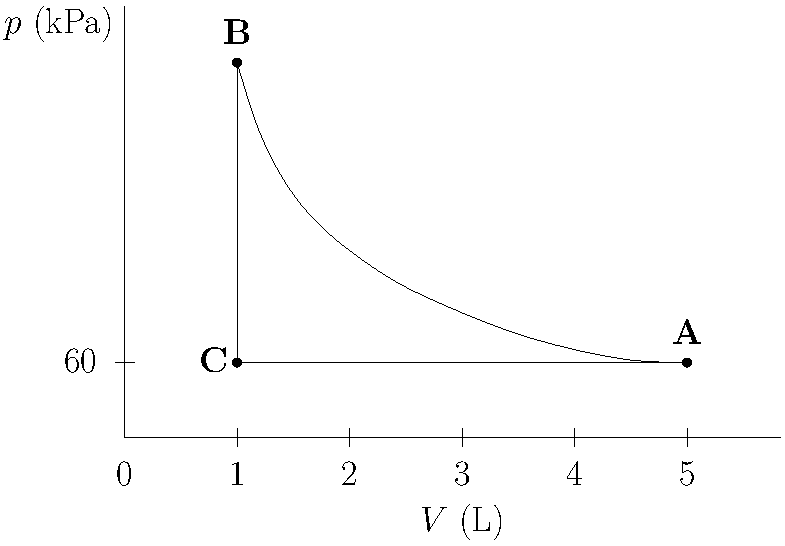
\includegraphics[width=3.0in]{gas_processes/cycle_w_isotherm_prob.pdf} 
%  \end{center} 
%   \caption{$p$-$V$ diagram for Problem \ref{prob:cycle_w_isotherm}}
%   \end{figure}
%\label{prob:cycle_w_isotherm}
%\end{problem}

%\begin{problem}
%An ideal gas with $\gamma = 1.4$ and $T = 300\units{K}$ starts at 
%point {\bf A} in Fig. It is   
%compressed adiabatically until its volume is $2.0\units{L}$ at {\bf B},
%and it is then cooled at constant pressure until it reaches $300\units{K}$
%at {\bf C}.  Finally it is allowed to expand isothermally back to 
%state {\bf A}.  Find 
%\begin{enumerate}
%\item the net work done on the gas, and 
%\item the minimum volume of the gas.
%\end{enumerate}
%\label{prob:}
%\end{problem}
%\newpage

%\begin{problem}
%A gas sample with the specific heat ratio $\gamma = 1.4$ undergoes 
%the cyclic process {\bf ABCA} shown in Fig. , where {\bf AB} is an adiabat. 
%The pressure at {\bf A} is $60\units{kPa}$.  Find 
%\begin{enumerate}
%\item the pressure at {\bf B}, and 
%\item the net work done on the gas.
%\end{enumerate}
%\begin{figure}[h]
%   \begin{center}
%   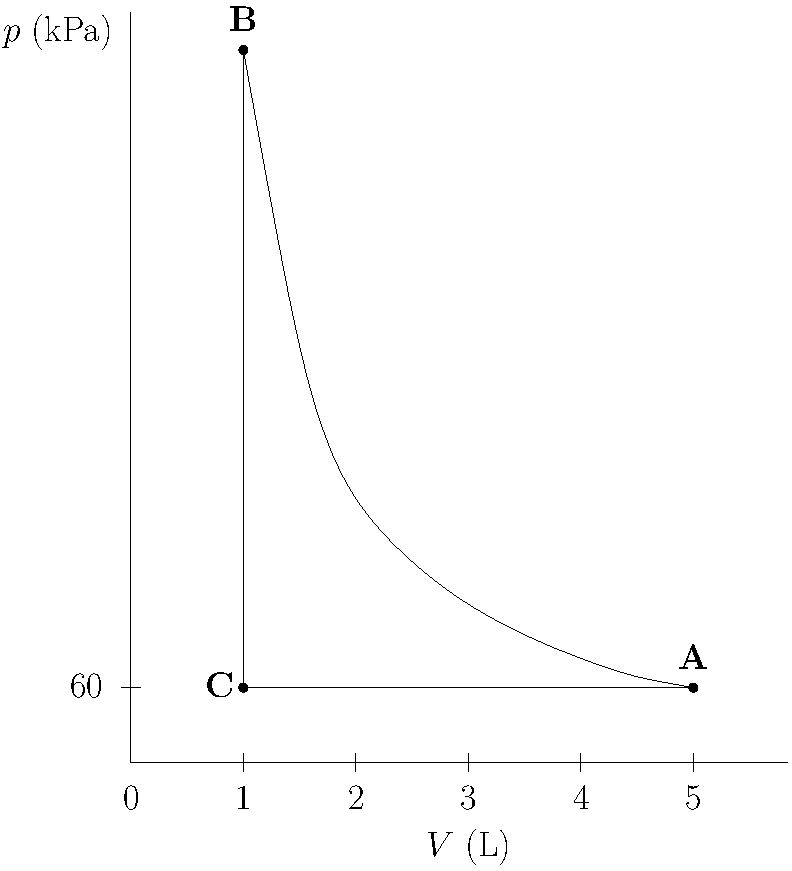
\includegraphics[width=2.5in]{gas_processes/cycle_w_adiabat_prob.pdf} 
%   \end{center} 
%   \caption{$p$-$V$ diagram for Problem \ref{prob:cycle_w_adiabat}}
%   \end{figure}
%\label{prob:cycle_w_adiabat}
%\end{problem}





%\input{gas_processes/test.tex}

%\chapter[Second Law and Entropy]{Second Law of Thermodynamics and  Entropy}
\label{chapter:second_law}


%\section*{Objectives}
%
%\begin{objectives}
%
%\item State and use the definitions of microstates, macrostates,
%  and multiplicity.  Understand the connection between multiplicity
%  and probability.
%
%\item Calculate the multiplicity of an Einstein solid or two
%  coupled Einstein solids.  Determine the temperature of an Einstein
%  solid.
%
%\item Understand the implications of the second law of
%  thermodynamics to heat flow and irreversibility.  Describe the
%  second law in terms of probability, multiplicity, and entropy. 
%
%\item State the definition of temperature and show that this
%  definition is consistent with the Clausius statement of the second
%  law.
%
%\end{objectives}

%\section{Introduction}

In this chapter we will discuss one of the most significant
developments in the history of science --- the development of a {\em
  statistical} theory of thermodynamics.  Here is the question: if a
chunk of ice, or a glass of water, or an air-filled balloon is composed of
$10^{22}$ or $10^{23}$ molecules, isn't it necessary to describe the
dynamics of each individual molecule?  To determine the force on each
molecule and solve Newton's second law to figure out its motion?  The
answer is no, thankfully.  Instead, we can treat each of these
molecules as though they are behaving randomly, and recover all the
results of thermodynamics from a probabilistic treatment.

%In this theory, the
%behavior that we observe happens because it is the most likely
%scenario.  At first glance, this might seem unreasonable; after all,
%the fact that a state is less likely doesn't mean that it can't
%happen, correct?  Yes, but when we consider systems with $10^{23}$
%molecules in it, it turns out that the more likely states are {\bf
%  overwhelmingly}\footnote{The word ``overwhelming'' doesn't even
%  begin to describe just how much more probably the most probable
%  states are.  If we said that these states are much, much, much,
%  much, much, much, ... more probable, we'd have to spend several
%  decades repeating the word ``much'' to begin to get even a hint of
%  the magnitude of the probability here.} more likely and the less
%likely states are {\bf overwhelmingly} less likely.  In fact, the odds
%are so {\bf ridiculously} weighted that we will say that the more
%likely states ``always'' happen and that the less likely states
%``never'' happen.

The importance of this statistical approach cannot be overstated.
The idea that we can treat thermodynamic systems probabilistically
led to a revolution in scientific thought that ranks up there
with Newton's development of classical physics, Pasteur's development
of germ theory of disease, Einstein's theory of relativity, and
the development of quantum mechanics (which you'll see in PHYS 212).

We will introduce statistical mechanics by revisiting the basic phenomenon
of heat flow, the spontaneous thermal energy transfer from hotter objects
to colder objects.  The direction of the heat flow is determined by what
is known as the {\it second law of thermodynamics.}  We can derive the
second law of thermodynamics from probability arguments; essentially,
thermal energy flow is dictated by moving from an improbable to a
probable situation.  Entropy is introduced as a measure of probability.
And along the way to understanding the second law, we will provide a
general definition of temperature.

\section{Heat Flow Revisited}

Consider the following process, illustrated in
Fig.~\ref{fig:paradigmatic_process}: a hot piece of metal is placed
into a container holding cold water.  As time passes, thermal energy
flows from the metal to the water, making the metal colder and the
water warmer.  Eventually, the two are at the same temperature and no
more thermal energy is transferred.  This is {\it heat\/}: the
spontaneous thermal energy transfer due to the temperature difference,
as we identified in section~\ref{section:heat}.

\begin{figure}
\begin{center}
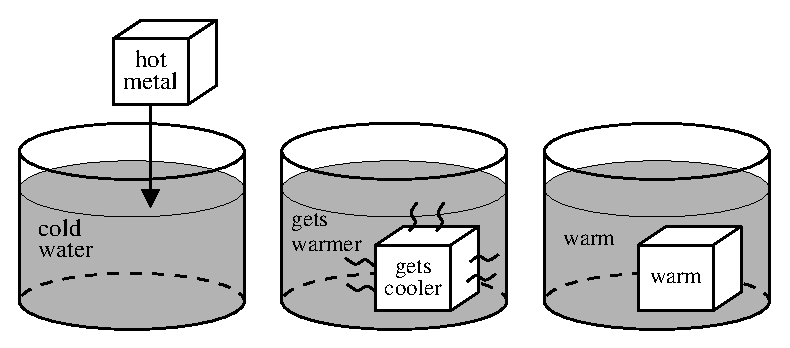
\includegraphics[width=4.6in]{second_law_and_entropy/paradigm}
\caption{A hot piece of metal is placed into cold water.  Thermal
  energy is transferred from the hot metal to the cold water until
  they are in thermal equilibrium.}
\label{fig:paradigmatic_process}
\end{center}
\end{figure}

In a heat flow scenario, such as this one, the first law of
thermodynamics states that energy is conserved, and so we must have
\begin{equation}
\Delta E_\text{therm,water} = -\Delta E_\text{therm,metal}.
\end{equation}
However, energy conservation would be equally well satisfied if the
heat flowed the other way.  Imagine putting the hot metal into cold
water and finding that the metal becomes increasingly hotter while the
water becomes increasingly cooler, beginning to freeze.  Absurd!  This
is never observed to happen.  And yet it would be perfectly consistent
with the first law of thermodynamics.

What this process illustrates is that there must be an additional law
of nature involved that determines the direction of heat flow.  In a
fit of creativity, physicists decided to call this the {\it second}
law of thermodynamics.  There are many equivalent ways to state the
second law.  We will begin with the {\it Clausius statement} of the
second law, since it is the most intuitive.

\boxittext{
{\sc 2nd Law of Thermodynamics (Clausius):}\\  \raggedright
Heat cannot flow spontaneously from a material at lower temperature to
a material at higher temperature.
}

Let's examine this.  First, note that the law is, at this point,
empirical, which means it is a statement about the observed behavior
of nature.  The second law rules out the absurd scenario whereby heat
flowed from the cold water to the hot metal.  But, note that the
second law makes no statement about whether the heat will actually
flow from the metal to the water.  According to the second law, this heat
flow is allowed, but not required.  That is exactly what we want from
a general law, since after all the metal and the water may or may not
be thermally coupled.

Temperature plays a crucial role in the second law, since the question
of whether heat is allowed to flow from $A$ to $B$ or instead from $B$
to $A$ is answered by the temperatures $T_A$ and $T_B$.  Temperature
plays the role of nature's traffic cop, enforcing thermodynamic
``one-way streets.''\footnote{However, nature needs no traffic court
  since its one-way streets, like its speed limit, are
  self-enforcing.}  The primary topic of this chapter is the
explanation of why temperature plays this role.

Another interesting aspect of the second law is the phenomenon of {\it
irreversibility.}  Many processes in nature are reversible.  A movie of
the flight of a ball thrown straight up into the air, turning around and
coming back down, looks the same whether played forward or backward.
This is because Newton's law are {\it reversible} as long as friction
is negligible.  But once heat flows from the hot metal to the cold
water, it will never spontaneously  flow back again.  A movie of the
process (with some thermometers used to make the temperature visible)
would look different played backward versus forward.  Physicists believe
the second law is the origin of any irreversibility observed in nature,
which is to say, the second law of thermodynamics plays a crucial role
in determining the direction of time flow.

Interestingly, the second law is unique among laws of physics.  Most
laws are simply inferred from the behavior of nature.  We don't know
why energy conservation happens; we just know it does.  The second law
is different because we can essentially derive it.  We know {\it why}
it happens.  It is ultimately a statement about probability: thermal
energy flows spontaneously from hotter objects to colder objects
because that brings the system to a state with a more 
likely arrangement of energy.  

The rest of this chapter is concerned with expanding our probabilistic
understanding of the second law and temperature.  
% For this purpose, we
% will need to develop the concepts of microstates, macrostates, and
% multiplicity. 

\section{Microstates, Macrostates, and Multiplicity}

To explain how probabilities work in thermodynamics --- and ultimately
to explain entropy and how it relates to the second law of
thermodynamics --- it is necessary to discuss some fundamental
concepts of probability.  We start with definitions of 
{\em microstates} and {\em macrostates}:

\boxittext{
A {\it macrostate} is a specification of the macroscopic state of the
system.  For example, the pressure, temperature, and number of moles
of an ideal gas would specify a macrostate.
\bigskip

A {\it microstate} is the detailed specification of the microscopic
state of the system.  In the ideal gas example, the microstate would
be precise values for the position and velocity of every single
molecule.
}

A macrostate can have many microstates associated with it.  In the
ideal gas example, there are many possible arrangements of the
molecules that are consistent with having, say, one mole of gas with
atmospheric pressure and room temperature.  This brings us to
multiplicity:

\boxittext{
The {\it multiplicity} $\Omega$ of a macrostate is the number of
microstates associated with that macrostate. 
}

Let's explore these ideas with a specific example: a pair of six-sided
dice, one red and one green.\footnote{Having dice of the same color
  wouldn't change anything.  We just use different colors to help
  label the dice.}  There are 36 possible outcomes of rolling these
dice, listed in Table~\ref{table:paradise}, and the sum of the two
dice can be any number between two and twelve.  Not every sum is
equally probable, however.   If you roll the dice many times, you will
notice you get a sum of seven much more often than, say, a sum of
twelve.

The 36 possible outcomes are the microstates.  The red dice showing
`5' and the green die showing `3' would be a particular microstate
(labeled 5-3 in Table~\ref{table:paradise}).  The sum of the dice,
eight in this case, represents a macrostate.  Notice that there are
many ways to roll a sum of eight; or stated another way, there are
multiple microstates associated with the macrostate `8.'  The number
of ways to roll an `8' is the multiplicity $\Omega$.  Looking at
Table~\ref{table:paradise}, we see there are five different ways to
roll an `8', so the multiplicity $\Omega =5$.

The multiplicity of a macrostate is useful to know because it tells us
the probability of obtaining that particular macrostate.  Each of the
36 microstates for a pair of dice is equally likely.  The reason that
a sum of seven is a more likely outcome than a sum of twelve is not
because 4-3 is more likely than 6-6 (it's not!), rather, there are
more ways to roll a `7.'

Now let's come back to physics.  The macrostate of a collection of
molecules  could be defined in terms of the number of particles and
the amount of energy $E_\text{therm}$ they have.  A microstate would
correspond to a particular arrangement of the energy among the
molecules.  Since there are many possible ways to arrange the energy
among the molecules, there are many microstates associated with this
macrostate.  The number of possible ways to arrange the given amount
of energy would then be the multiplicity $\Omega$.

\begin{table}
\begin{center}
\begin{tabular}{clcl}
\hline\hline
sum & rolls (red die--green die) & $\Omega$ & probability \\
\hline
2 & 1-1 & 1 & 1/36 \\
3 & 1-2 \quad 2-1 & 2 & 2/36 = 1/18 \\
4 & 1-3 \quad 2-2 \quad 3-1 & 3 & 3/36 = 1/12 \\
5 & 1-4 \quad 2-3 \quad 3-2 \quad 4-1 & 4 & 4/36 = 1/9 \\
6 & 1-5 \quad 2-4 \quad 3-3 \quad 4-2 \quad 5-1 & 5 & 5/36 \\
7 & 1-6 \quad 2-5 \quad 3-4 \quad 4-3 \quad 5-2 \quad 6-1 & 6 & 6/36 = 1/6 \\
8 & 2-6 \quad 3-5 \quad 4-4 \quad 5-3 \quad 6-2 & 5 & 5/36 \\
9 & 3-6 \quad 4-5 \quad 5-4 \quad 6-3 & 4 & 4/36 = 1/9 \\
10 & 4-6 \quad 5-5 \quad 6-4 & 3 & 3/36 = 1/12 \\
11 & 5-6 \quad 6-5 & 2 & 2/36 = 1/18 \\
12 & 6-6 & 1 & 1/36 \\
\hline\hline
\end{tabular}
\caption{The 36 possible results from rolling a pair of dice (one
  red, one green).}
\label{table:paradise}
\end{center}
\end{table}
  
To go from multiplicity to probability we need one more piece of
information.  In the case of the dice, each of the 36 possible
outcomes was equally likely, assuming that the dice were fair,
returning each of the six values with equal probability.  Does this
apply as well for our system of $N$ particles sharing a total energy
$E_\text{therm}$?  In general, we cannot prove this, but to make
progress we will assume that it is true.

\boxittext{\raggedright
{\sc The Fundamental Assumption of Statistical Mechanics:}\\
All of a system's accessible microstates are equally likely.
}

``Accessible microstates'' here means simply those which are allowed by
energy conservation.  The motivation for this assumption is that
whatever the specific dynamics are, however the molecules are
colliding and sloshing energy back and forth among each other, they
eventually visit every possible state allowed by energy conservation.
So a sequence of snapshots of the system would look like randomly
selected examples of possible microstates.   In the end, nature has
confirmed that starting with the fundamental assumption leads to
predictions that match experiments extremely well.  Now we shall see
what the fundamental assumption buys us.

\section{Einstein Solid}

We now develop the ideas of the previous section in the context of a
specific model.  The simplest model to work with, it turns out, is not
the ball-spring model or the ideal gas, but rather a variation of the
ball-spring solid called the Einstein solid.  Experiments on very cold
metals showed that their specific heats could fall well below the
value $3R$, suggesting something not contained in the ball-spring
model was occurring at low temperatures.  Einstein showed that a
quantum mechanical version of the ball-spring model could explain this
result.\footnote{The complete description of very cold metals requires
  an additional modification, worked out by a Dutch physicist named
  Peter Debye.  We will not consider the Debye theory here.}  To
begin, notice that a three-dimensional oscillator, such as the
molecule in the ball-spring model, can be written as a sum of three
independent, one-dimensional oscillators:
\begin{align}
E_\text{ball} &= \bigl(\textstyle\frac{1}{2} m v_x^2 + \frac{1}{2} m v_y^2 
+ \frac{1}{2} m v_z^2\bigr) +
\bigl(\textstyle\frac{1}{2} k_{sp} x^2
+ \frac{1}{2} k_{sp} y^2 + \frac{1}{2} k_{sp}z^2\bigr)
\nonumber\\[1.5ex]
 &= \bigl(\textstyle\frac{1}{2}mv_x^2+
   \frac{1}{2}k_{sp}x^2\bigr)
+\bigl(\textstyle\frac{1}{2}mv_y^2+\frac{1}{2}k_{sp}y^2\bigr)
+\bigl(\textstyle\frac{1}{2}mv_z^2+\frac{1}{2}k_{sp}z^2\bigr)
\end{align}
In the second grouping, each term in parentheses is an oscillator
moving in one particular direction and independent of the motion in
the other perpendicular directions.  Thus a set of $N$ molecules in
the ball-spring model is equivalent to $3N$ one-dimensional
oscillators.  In what follows we will be working primarily with the
one-dimensional oscillators so we let $N$ represent the number of
oscillators instead of the number of molecules.  The number of
molecules is then $N/3$.

Einstein proposed to treat the one-dimensional oscillators quantum
mechanically, which should be appropriate when the temperature is
low enough.  We will not discuss quantum mechanics here --- that is a
topic for PHYS 212 --- but we will summarize the main results of interest
to us.  The energy levels of the quantum harmonic oscillator are not
continuous but rather discrete (or {\it quantized\/}).  This is
illustrated in Fig.~\ref{fig:qho}.  At very low energies we cannot
vary the oscillator energy up or down by arbitrarily small amounts,
but rather can only add energy in discrete chunks.  Furthermore, for
the quantum harmonic oscillator, these energy levels are equally
spaced.  Therefore we can write the energy level of an oscillator as
\begin{equation}
E_\text{osc} = E_0 + n\epsilon \qquad
\text{where $n=0$, 1, 2, 3, \dots}
\end{equation}
Here $E_0$ is the lowest energy level possible, and we may increase
the energy by adding an integer number of ``energy units'' of size
$\epsilon$. 

\begin{figure}
\begin{center}
\includegraphics[width=2in]{second_law_and_entropy/qho}
\caption{The quantum harmonic oscillator has discrete energy levels,
  shown as horizontal lines.  The energy difference between successive
  levels is $\epsilon$.}
\label{fig:qho}
\end{center}
\end{figure}

Now consider a system of two oscillators, with a total energy of three
``energy units.''  These oscillators bounce energy back and forth and
so one of the oscillators may have at a given instant anywhere from
zero to all three of the energy units.  Let $n_1$ be the number of
energy units that the first oscillator has, and $n_2$ the number of
energy units for the second oscillator.  Specifying $n_1$ and $n_2$
determines a particular microstate.  The total energy of three units
implies $n_1+n_2=3$, so the possible microstates, written as
$(n_1,n_2)$, are
\[
(3,0), \quad (2,1), \quad (1,2), \quad (0,3).
\]
Evidently, the multiplicity of the macrostate with two oscillators and
a total of three energy units is $\Omega =4$.  That is, there are four
different microstates with this total energy.

\begin{example}{Three oscillators, two energy units}
  Write down all the microstates for a system of three oscillators and
  a total of two energy units, and determine the multiplicity.
  \solution 
  For microstates written as $(n_1,n_2,n_3)$, we need to have
  $n_1+n_2+n_3=2$, so the possible microstates are
\[
(2,0,0),\quad(0,2,0),\quad(0,0,2),\quad
(1,1,0),\quad(1,0,1),\quad(0,1,1),
\]
and the multiplicity $\Omega=6$.
\label{example:multiplicity}
\end{example}

It is feasible to determine the multiplicity directly by counting the
microstates when the number of oscillators and energy units is small.
But this becomes unwieldy very quickly as the number  of oscillators
and energy units is increased.  Fortunately, we can derive the general
result for $N$ oscillators and $q$ total energy units, which is
\begin{equation}
\Omega = \frac{(q+N-1)!}{q!\;(N-1)!}.
\label{eq:Einstein_multiplicity}
\end{equation}
The factorial function is defined as $n!=n(n-1)(n-2)\cdots 2\cdot 1$.
For example, $5!=5\cdot 4\cdot 3\cdot 2\cdot 1=120$.  A special
case is the factorial of the number zero:  by definition, 
$0!=1$.  The meaning of $n!$ is that it is the number of
distinct ways to order $n$ objects.  The number of ways to order zero
objects is taken to be 1.

\begin{example}{Checking the multiplicity formula.}
Verify the Einstein solid multiplicity formula,
Eq.~(\ref{eq:Einstein_multiplicity}), for the cases of two oscillators
with three energy units and three oscillators with two energy units.
\solution
For two oscillators and three energy units ($N=2$ and $q=3$) the
multiplicity formula gives
\begin{equation}
\Omega = \frac{(3+2-1)!}{3!\;(2-1)!} = \frac{4!}{3!\;1!} =
\frac{24}{6\cdot 1} = 4,
\end{equation}
which matches our result above.  For the second case, $N=3$ and $q=2$,
giving
\begin{equation}
\Omega = \frac{(2+3-1)!}{2!\;(3-1)!} = \frac{4!}{2!\;2!} = \frac{24}{2^2}
= 6,
\end{equation}
verifying the second case.
\end{example}

Factorials become very large very quickly.  For example, $100!\approx
10^{157}$, which is an amazingly large number.  An Einstein solid with
100 oscillators and 200 energy units has a multiplicity $\Omega =
2.8\times 10^{82}$.  Now you can appreciate having
Eq.~(\ref{eq:Einstein_multiplicity}) to work with instead of counting
all possible microstates.  And imagine how large the result would be
for Avogadro's number of oscillators!

\section{Coupled Einstein Solids}

Our original goal was to understand heat flow.  That is, why thermal
energy spontaneously goes from hotter objects to colder objects.  To
that end, we will now consider two Einstein solids, solid $A$ with a
number $N_A$ oscillators and $q_A$ energy units, and solid $B$ with
$N_B$ oscillators and $q_B$ energy units.  If solids $A$ and $B$ are
brought into thermal contact, then they will be able to pass energy
units back and forth while maintaining a fixed total
$q_\text{tot}=q_A+q_B$.  But which way will the energy go, on average?  And
when will it come to thermal equilibrium?  Let us try to address these
questions. 

Once the two Einstein solids are thermally coupled and exchanging
energy, $A$ and $B$ should be regarded as {\it subsystems} of the
combined system.  For a particular division of energy among the two
subsystems, we have a multiplicity $\Omega_A$ that depends on $N_A$
and $q_A$, and a multiplicity $\Omega_B$ that depends on $N_B$ and
$q_B$.  

How do we calculate the combined multiplicity of the system?  If you
have three pairs of pants and five shirts, then you have $3\cdot 5=15$
possible combinations you can make, at least in polite company.
Similarly, subsystem $A$ may be in any of the number $\Omega_A$
microstates and subsystem $B$ in any of $\Omega_B$ microstates, so the
number of paired microstates we can make is the product $\Omega_{AB} =
\Omega_A\Omega_B$.  This is the combined multiplicity of the system.

Let's consider a specific case.  Let $N_A=3$ and $N_B=3$, and
$q_\text{tot}=q_A+q_B=6$.  The two systems may divide up the six energy
units a variety of ways, as shown in Table~\ref{table:two_systems}.
For each choice, the multiplicities $\Omega_A$ and $\Omega_B$ and the
combined multiplicity $\Omega_{AB}$ are given.  Note that the most
probable arrangement of energy, the one with the largest multiplicity,
is the one with three energy units in each subsystem.  If subsystem
$A$ started with zero energy units and subsystem $B$ with six units,
then simple random energy exchanges would move the coupled systems
toward the more probable state with $q_A=q_B=3$.  This is a clue about the
origin of the second law.

\begin{table}
\begin{center}
\begin{tabular}{ccrrr}
\hline\hline
$q_A$ & $q_B$ & \qquad $\Omega_A$ & $\Omega_B$ & \qquad $\Omega_{AB}$ \\
\hline
0 & 6 & 1 & 28 & 28 \\
1 & 5 & 3 & 21 & 63 \\
2 & 4 & 6 & 15 & 90 \\
3 & 3 & 10 & 10 & 100 \\
4 & 2 & 15 & 6 & 90 \\
5 & 1 & 21 & 3 & 63 \\
6 & 0 & 28 & 1 & 28 \\
\hline\hline 
\end{tabular}
\caption{Possible macrostates for system $A$ and $B$ sharing six units
  of energy, with $N_A=3$ and $N_B=3$.}
\label{table:two_systems}
\end{center}
\end{table}

From Table~\ref{table:two_systems} we see that the most probable
situation is only slightly more probable than the other possibilities.
This changes dramatically as the system size is increased.  In
Fig.~\ref{fig:multiplicity_with_size} we plot the combined
multiplicity as a function of $q_A$ for various numbers of oscillators
and energy units.  As the figure shows, when the numbers become
larger, say in the thousands, the multiplicity function becomes 
sharply peaked.  Some particular division of energy between
the two subsystems is vastly, hugely, awesomely, mind-bogglingly more
probable\footnote{I.e., it isn't just a little more probable, it is a
  {\bf lot} more probable.} than all others.  This we identify as the
equilibrium division of energy.  Now imagine what occurs when you
approach Avogadro's number of energy units.  The multiplicity function
becomes completely sharp.  There is some particular division of the
energy between subsystems $A$ and $B$ that is ridiculously, 
overwhelmingly, staggeringly\footnote{``\dots vastly, hugely,
  awesomely, mind-bogglingly, ...'' and that doesn't even begin to cover it!}
more probable than any other.

\begin{figure}
\begin{center}
\includegraphics[width=5in]{second_law_and_entropy/multiplicity_with_size.eps}
\caption{Plots of the multiplicity as a function of $q_A$ for a
  variety of system sizes.  Note that $q_B$ is determined by
  $q_A+q_B=q_\text{tot}$.} 
\label{fig:multiplicity_with_size}
\end{center}
\end{figure}

Now we have the probabilistic origin of the second law.  Subsystems
$A$ and $B$, before they are thermally coupled, can be prepared with
any thermal energy we would like.  We made the metal object hot and
the water cold before plunging the metal into the water.  But once the
subsystems are thermally coupled, they will move from whatever
division of energy they started with toward the maximally probable
arrangement of energy for the coupled system.  They are irresistibly
led to it by essentially random exchanges of energy between the
subsystems.  The energy transferred along the way is what we had
previously identified as heat.

To summarize:

\boxittext{
The second law of thermodynamics is a result of a system prepared in
an improbable initial state then moving to a vastly more probable
final state.}
\break
{\bf This is an incredibly important result!!!!}  With this
statement, we don't have to worry at all about the detailed,
Newtonian mechanics of the (many, many) individual molecules or
atoms in a solid, liquid or gas.  We treat all the motion as though
it is random and then simply figure out the probabilities.  

\section{Entropy}

Entropy is part of the title of the chapter; perhaps it is time we
introduced it.  The fact is, we have already been discussing the
entropy, because entropy is simply the multiplicity cast into a more
convenient form, by means of a logarithm.  We define entropy as
\begin{equation}
S = k_B\ln\Omega.
\label{eq:entropy_def}
\end{equation}
The factor of Boltzmann's constant plays little role here, apart from
giving entropy units (which are J/K).\footnote{By the way, Boltzmann
was the one who realized that the second law had a probabilistic origin,
and Eq.~(\ref{eq:entropy_def}) is engraved on his tombstone.  Check it
out if you're ever in Vienna.}  The logarithm is a monotonic function,
which means that the larger $\Omega$ gets, the larger $S$ gets.  So being
the most probable state is the same as being the highest entropy state.
This is a really important statement, so important that we will elevate
it to box-dom:

\boxittext{Entropy is a measure of probability:  the more probable a
state, the higher its entropy.}
\break
Entropy is often incorrectly described as a measure of the disorder
of a system.  This is simply not true; entropy is measure of
probability and probability only.  It {\bf is} true that higher
entropy states are often more disordered than lower-entropy states,
but this is not always true; there are many examples
%have been several experiments recently 
of systems that become {\bf more} ordered as their
entropy increases.

We can now write the second law of thermodynamics rather concisely as
a statement of probability, given in the boxed statement at the end of
the previous section:
\begin{equation}
\Delta S_\text{total} \geq 0. \qquad\text{(Entropic version of 2nd law)}
\end{equation}
Starting from some initial state that is not the maximum entropy
state, the combination of all our subsystems will exchange thermal
energy and move spontaneously toward the maximum entropy state.  And
for large systems, it moves irreversibly: there is a negligibly small
probability of moving away from the maximum entropy state
(think about the sharply peaked multiplicity).

Note that the entropic form of the second law refers to the {\bf total}
entropy of a system, i.e., the {\bf total} entropy cannot decrease.
But the entropy of part of a system {\bf can} decrease.  So, for
instance, it is very possible to have a chemical reaction where
the stuff inside your beaker ends up with a lower entropy,
as long as there is a corresponding increase in entropy somewhere
else (most likely in the air around the beaker whose entropy
increases when heated up by heat flowing from the beaker).

We could have expressed all this with the multiplicity, so why
take a logarithm and call it entropy?  There are three reasons.  First,
since multiplicities become very, very large for even modest sized
systems, we find more workable expressions if we use the
logarithm.  For example, in the previous case of 100 oscillators with
200 energy units, we get an entropy of
\begin{equation}
 S/k_B = \ln\Omega = \ln\left(\frac{299!}{200!\;99!}\right) = 190 ,
\end{equation}
which is much nicer to manipulate and plot than $10^{82}$.

The second reason is that the combined entropy of two systems is
simply the sum,
\begin{equation}
S_{AB} = S_A + S_B,
\end{equation}
which you will show in Problem~\ref{problem:entropy_additive}.  When we
are trying to identify the maximum entropy state, we can combine the
contributions $S_A$ and $S_B$ from subsystems $A$ and $B$ by simply
adding them together (like we would for energies).  That will turn out
to be handy now as we finally come to the definition of temperature.

The third reason is historical: it so happens that entropy was defined
by Clausius a few years before Boltzmann developed a probabilistic
theory for thermodynamics. Clausius defined the quantity that he
called {\em entropy}\footnote{Clausius chose the word {\em entropy}
  partially after the Greek word {\em trope} which means {\em
    transformation} and partially because he wanted a word that
  sounded similar to {\em energy} since he defined entropy in terms of
  an energy flow.}  in terms of energy flow in a thermodynamical
system (to be discussed in the next chapter).  He even stated the
entropic form of the second law of thermodynamics, though no one
at the time understood that this is really a statement of probability.
So, taking the logarithm of multiplicity was needed to keep the
entropic statement of the second law consistent with that proposed by
Clausius.

%One more comment about entropy and the second law:  you might
%wonder why we can say that the total entropy of a system {\em never}
%decreases.  After all, you might think, if entropy is a measure
%of probability (which it is), couldn't a system move (perhaps 
%momentarily) to a less probable state, resulting in an overall
%entropy decrease?  Theoretically, the answer is ``yes'', but for
%real, macroscopic systems with $N \approx 10^{23}$, the less
%probable (lower entropy) states are so incredibly, unfathomably,
%inconceivably\footnote{... and so on (see ``vastly, hugely,
%mind-bogglingly, ...'' from previous section)} less probable that
%we say that it will ``never'' happen.  Here is another advantage
%of the use of the logarithm in the definition of entropy:  when you
%take the logarithm of ridiculously large multiplicities, any
%reasonable decrease in the multiplicity isn't even registered
%as a blip in the entropy (see problem \ref{prob:natural_log} at
%the end of this chapter).

\section{The Definition of Temperature}

As we discussed in Chapter \ref{chapter:thermal_energy}, 
temperature is often defined in terms of the thermal kinetic energy.
Certainly thermal kinetic energy and temperature are related, via the
equipartition theorem, so it is a useful and convenient picture to
have.  But defining temperature this way leaves its most fundamental
role --- namely, that it is the traffic cop dictating which way
thermal energy will spontaneously flow --- completely unexplained.  In
this section we will introduce a definition of temperature that
naturally explains its presence in the Clausius statement of the
second law.  Conveniently, this {\it second law temperature} turns out
to be the same temperature we know and love from the ideal gas law,
the equipartition theorem, and the ball-spring solid.

Let's think of the entropy of a system as a function of its thermal
energy.  Adding more thermal energy to a system gives more ways to
distribute the energy, and so increases the multiplicity.  This means
an increase in entropy, so $S$ should be an increasing function of
$E_\text{therm}$.  A typical dependence of entropy on $E_\text{therm}$
is shown in Fig.~\ref{fig:entropy_vs_energy}.  Note that the entropy
is increasing with $E_\text{therm}$, but also note that the rate of
increase slows down with increasing energy.  That is, the slope is
steadily decreasing as $E_\text{therm}$ increases.  This can be
understood as a type of diminishing returns: systems with very low
$E_\text{therm}$ can gain a lot of multiplicity by adding energy.
Once the thermal energy is high, additional thermal energy has less
impact on the entropy.

\begin{figure}
\begin{center}
\includegraphics[width=3.5in]{second_law_and_entropy/entropy_vs_energy}
\caption{Entropy as a function of thermal energy.}
\label{fig:entropy_vs_energy}
\end{center}
\end{figure}

Now let's couple two subsystems, $A$ and $B$.  The combined energy is
fixed, $E_\text{total} = E_A + E_B$.  Consequently, as system $A$
gains energy, system $B$ loses energy, and vice-versa.  In
Fig.~\ref{fig:coupled_systems} we plot both $S_A$ and $S_B$, but
notice that the $S_B$ curve is flipped over left to right.  This is
because $E_B=0$ occurs at the right side of the plot, where $E_A$ is
at its maximum, and $E_B$ increases as you move to the left.  The
reason for plotting it this way is that we can, for a particular
choice of $E_A$, read off both $S_A(E_A)$ and $S_B(E_B)$.  Also shown
on the plot is the combined entropy $S_\text{total}=S_A+S_B$.


\begin{figure}
\begin{center}
\includegraphics[width=4.5in]{second_law_and_entropy/coupled_systems.eps}
\caption{Entropies of subsystems $A$ and $B$, as well as the combined
system entropy $S_\text{total}$, all plotted versus $E_A$.}
\label{fig:coupled_systems}
\end{center}
\end{figure}

Now imagine starting with a relatively small value of $E_A$, where the
heavy lines are drawn on the left.  What would be the net effect on
the entropy if we were to take some energy from system $B$ and give it
system $A$?  The plot shows that $S_B$ would decrease and $S_A$ would
increase.  The plot also shows that, since the $S_A$ curve in this
region is steeper than the $S_B$ curve, system $A$ would gain 
more entropy than system $B$ would lose.  In other words,
$S_\text{total}$ would increase.  Therefore, the ``force'' of
probability pushing towards a (vastly) more probable state dictates
that energy flows from system $B$ to system $A$.

What the previous analysis should make clear is that the question of
which way the energy will flow is determined by the magnitude of the
{\it slope\/} on an entropy versus energy graph.  Whichever system,
$A$ or $B$, has the steeper slope will be the one to receive the
energy.

Let's carry this analysis further.  After some energy has flowed from
$A$ to $B$, we find that $E_A$ has increased to where the second set
of heavy lines are drawn.  Here, the slopes of the $S_A$ and $S_B$
curves are equal in magnitude and opposite in sign.  Any entropy
change of system $A$ is canceled by the entropy change of system $B$,
so there is no longer entropy gained by increasing $E_A$ (or
decreasing it).   Thermal energy will no longer be transferred because
we are at the maximum combined entropy, which can be seen from the
plot of $S_\text{total}$, and we have reached thermal equilibrium.
Any additional transfer of energy (in either direction) will
result in a decrease in total entropy.

All this discussion leads to the notion that the slope
$dS/dE_\text{therm}$ is directing the thermal energy traffic.
Whichever subsystem has the smaller slope will give up energy to the
subsystem which has the larger slope.  Hence, we define temperature as

\boxiteq{
\begin{equation}
\frac{1}{T} \equiv \frac{dS}{dE_\text{therm}},
\label{eq:temperature_def}
\end{equation}}

\noindent and our probability analysis becomes equivalent to the Clausius
statement.

This definition, then, explains the role of temperature in the second
law, but does it match our previous notions of temperature?  And what
does it mean intuitively?  First, yes, it does match the ideal gas
temperature, etc.  This can be shown by deriving the equipartition
theorem from this definition of temperature; all our previous uses for
temperature (such as the ideal gas) had their origin in the
equipartition theorem.

As for an intuitive meaning, think of it this way: inverse temperature
(that is, $1/T$) is a measure of how much use a system has for
energy.  When a system can find many ways to divide up the energy,
then adding some energy will increase $S$ a lot.  That is a low
temperature system.  A high temperature system is one where
diminishing returns has set in, and additional energy does not result
in a substantial entropy increase.

Finally, note that for large systems we can add some amount of energy
without significantly changing the temperature (for example, adding 10
joules of thermal energy to a cup of water).  In this case, we can
approximate Eq.~(\ref{eq:temperature_def}) as
\begin{equation}
\frac{1}{T} \approx \frac{\Delta S}{\Delta E_\text{therm}} 
\qquad\text{or}\qquad
T \approx  \frac{\Delta E_\text{therm}}{\Delta S}.
\label{eq:temperature_approx}
\end{equation}
This is often a handy way to {\em estimate} temperature from entropy change
or vice-versa.

\begin{example}{The Temperature of my Coffee}
Adding $50\units{J}$ of thermal energy to my coffee cup caused its
entropy to increase by an amount of $0.17\units{J/K}$.  Estimate the
temperature of my coffee.
\solution
According to Eq.~(\ref{eq:temperature_approx}) we have
\begin{equation}
T \approx  \frac{\Delta E_\text{therm}}{\Delta S} = 
\frac{50\units{J}}{0.17\units{J/K}} = 294\units{K}.
\end{equation}
That's room temperature.  Yuck!
\end{example}

\newpage

\section*{Problems}
\markright{PROBLEMS}

\begin{problem}
Consider an Einstein solid with three oscillators and four units of
energy.
\begin{enumerate}
\item Calculate the multiplicity for this macrostate.
\item Write out the triplet for each possible microstate.  For
  example, the microstate where the first oscillator has all the units
  of energy can be written as $(4,0,0)$.  Confirm that you find the
  correct number of microstates.
\end{enumerate}
\label{prob:multiplicityforthree}
\end{problem}

\begin{problem}
Calculate the multiplicity of an Einstein solid with 24 oscillators
and 15 energy units.  
\label{prob:mult_of_twentyfour}
\end{problem}

\begin{problem}
Suppose you roll a fair six-sided die three times in a row.
\begin{enumerate}
\item Determine the probability of getting exactly the sequence 1--3--2?
\item Now determine the probability of getting any other particular
sequence (hint: no calculation necessary).
\item What is the probability of rolling a sum of 6?
\end{enumerate}
\label{prob:rolldie}
\end{problem}

\begin{problem}
  For two Einstein solids with $N_A=3$ and $N_B=3$ and six energy
  units, how many times more probable is the macrostate with equally
  shared energy than the macrostate where system $A$ has all the
  energy?  Use Table~\ref{table:two_systems}.
\label{prob:twosolids}
\end{problem}

\begin{problem}
Is it really true that the entropy of an isolated system consisting of
two Einstein solids never decreases?  Consider a pair of very small
solids.  Explain why this statement is more accurate for large systems
than for small systems.
\end{problem}

\begin{problem}
A large object's entropy is observed to increase by $0.15\units{J/K}$
when we add $45\units{J}$ of thermal energy.  Assume that this causes
a negligible increase in the temperature of the object.  Determine
the approximate temperature of the object.
\label{prob:tempoflargeobject}
\end{problem}

\begin{problem}
  The idea of ``diminishing returns'' says that while the entropy does
  increase with increasing thermal energy, the slope is decreasing
  (see Fig.~\ref{fig:entropy_vs_energy}).  The Einstein solid
  multiplicity, like most materials, shows this behavior.  Here is how
  to see it:
  \begin{enumerate}
  \item For an Einstein solid with 10 oscillators and 5 energy units,
    calculate how much the entropy increases, i.e. $\Delta S$, if you
    add one more energy unit (you may leave your answer in terms of
    $k_B$).
  \item Now consider an Einstein solid with 10 oscillators and 15
    energy units, and calculate how much the entropy increases if you
    add one more energy unit.
  \item Do your answers to (a) and (b) confirm the diminishing
    returns?  Explain why.
\end{enumerate}
\label{prob:diminishing}
\end{problem}

\begin{problem}
For two Einstein solids $A$ and $B$, the entropy as a function of
thermal energy is given by 
\[
S_A= k_B\, 400\ln(E_A/300) \qquad S_B = k_B\, 100\ln(E_B/800)
\]
where $E_A$ and $E_B$ are the thermal energies of systems $A$ and
$B$.  If the two solids are brought to thermal equilibrium, what
relation, if any, can be made between the final energies $E_{A,f}$ and
$E_{B,f}$? 
\label{prob:entropyoftwosolids}
\end{problem}

\begin{problem}
Consider a very strange system whose multiplicity is $\Omega_A=1$
regardless of how much energy it has.  Imagine starting this system
with some amount of energy and bringing it into thermal contact with
system $B$, an Einstein solid.
\begin{enumerate}
\item In which direction will the energy flow, or will no energy flow?
\item What can you say about the energies of the final state?  For
  example, will they be equal?  If they are unequal, which is larger?
  Is there anything more you can conclude?
\end{enumerate}
\label{prob:strangesystem}
\end{problem}

%\begin{problem}
%The multiplicity of a monatomic ideal gas is given by $\Omega =
%c(E_\text{therm})^{3N/2}$, where $c$ is some constant that depends on
%the number of particles and volume, but does not depend on
%$E_\text{therm}$.  (Note: we will derive this result in
%Chapter~\ref{chapter:heat_engines}.) 
%\begin{enumerate}
%\item Use this multiplicity to find the entropy of an ideal gas.
%\item Use your result from part (a) and the definition of temperature
%  to derive the relation $E_\text{therm}=\frac{3}{2}Nk_BT$.  Hint: use
%  the logarithm properties $\ln(xy) = \ln x + \ln y$ and $\ln(x^n) =
%  n\ln x$.
%\end{enumerate}
%\end{problem}
%
%\begin{problem}
%There is no problem 10.
%\end{problem}

\begin{problem}
A substance has entropy $S=c\sqrt{E_\text{therm}}$, where $c$ is
  some constant.  Use the definition of temperature to find
  $E_\text{therm}$ as a function of $T$.
\end{problem}

\begin{problem}
Consider two Einstein solids with $N_A=3$ and $N_B=3$ and eight energy
units. 
\begin{enumerate}
\item Make a table like Table~\ref{table:two_systems}.  Note that many
  of the multiplicities you will need are already in
  Table~\ref{table:two_systems}, so there is no need to re-calculate
  everything. 
\item How many times more probable is the macrostate with equally
  shared energy than the macrostate where system $A$ has all the energy?
\end{enumerate}
\end{problem}

\begin{problem}
An Einstein solid has four oscillators and three units of energy.
\begin{enumerate}
\item Calculate the multiplicity of the solid.
\item Identify all the possible microstates using the parenthesis
  notation of Example~\ref{example:multiplicity}.
\end{enumerate}
\end{problem}

\begin{problem}
System $A$ and system $B$ are both large.    For system $A$, adding
$250\units{J}$ of thermal energy causes an entropy increase of
$0.80\units{J/K}$.  For system $B$, adding $250\units{J}$ of thermal
energy causes an entropy increase of $0.60\units{J/K}$.
\begin{enumerate}
\item Without mentioning temperature, use probability arguments to
  determine which way thermal energy will flow when systems $A$ and
  $B$ are thermally coupled.
\item Estimate the temperature of each object and check that your
  result is consistent with part (a).
\end{enumerate}
\end{problem}

\begin{problem}
Show that $S_{AB} = S_A + S_B$ follows from the definition of entropy.
\label{problem:entropy_additive}
\end{problem}

%\begin{problem}
%To get an idea of what the logarithm does to the definition of 
%entropy, let's try a simple calculation.  
%\begin{enumerate}
%\item Assume that you have
%a multiplicity $\Omega = 10^{10}$.  Take the natural log
%of this multiplicity and write down the entropy (as a multiple
%of Boltzmann's constant $k_B$) to five decimal places, i.e., 
%``S = ??.?????$k_B$.''
%Now, subtract 1 from your multiplicity (i.e. 9999999999) and take the natural
%log of that, and write it down the new entropy (as a multiple
%of $k_B$) to five decimal places.  Is there
%a noticeable drop in entropy due to the small drop in multiplicity?
%\item Repeat part (a), but this time subtract 10 from the multiplicity.
%Then do it again, subtracting 100, 1000, etc, until you finally
%see an entropy decrease that is noticeable to five decimal
%places.
%\item Write a few sentences explaining why total entropy is never
%observed to decrease in a real system (with $N \approx 10^{23}$),
%even though the multiplicity {\bf can} decrease slightly.
%\end{enumerate}
%\label{prob:natural_log}
%\end{problem}

\begin{problem}
Entropy applies to more than just heat flow.  We can use entropy
and the second law of thermodynamics to discuss movement of
air in a room.
\begin{enumerate}
\item Consider a room with only 100 gas molecules.  Theoretically,
the gas molecules can move anywhere in the room.  Calculate the 
probability that all 100 of the molecules will be found on
one particular side of the room.
\item Now, consider a real room with a realistic amount of gas in
it -- let's say that there are $10^{26}$ gas molecules in the room.
Calculate the probability that all of these gas molecules will
be found in one particular side of the room.  (Note:  the probability
is {\bf so} small that your calculator or computer might simply
give ``0'' for the answer.)
\item Is it reasonable to say that you will ``never'' find all the
air in one side of the room?
\item Now, write a couple of sentences explaining why it is
(from a probability perspective) that when a perfume bottle is
opened, the scent of the perfume will spread throughout
the room.  
\item After the perfume smell has spread throughout the room,
would you expect all of the perfume molecules to go back
into the bottle?  Discuss this using the entropic form of the
second law of thermodynamics.
\end{enumerate}
\end{problem}
\newpage

\begin{problem}
The graphs in the figure below give plots of entropy $S$ vs.\ $E_\text{therm}$ for
two different solids, A and B.  Solid A starts with indicated energy $E_A$ and 
entropy $S_A$, and Solid B starts with $E_B$ and $S_B$.  
When Solid A has energy $E_A$, the slope of the entropy 
vs.\ energy curve is $dS_A/dE= 0.2\units{K$^{-1}$}$, and 
when Solid B has energy $E_B$, the slope of the entropy vs.\ energy 
curve is $dS_B/dE = 0.4\units{K$^{-1}$}$.

\begin{figure}[h]
\begin{center}
\includegraphics[width=5.0in]{second_law_and_entropy/energy_transferA.eps}
\caption{Figure for Problem \ref{prob:energy_transferA}}
\label{fig:energy_transferA}
\end{center}
\end{figure}

The two solids are brought into thermal contact with each other so that
energy can flow between them.
\begin{enumerate}
\item Which way will the energy flow:  from A to B, from B to A, or 
will no energy flow?  Give  qualitative reasoning to support your answer.
\item Now let's get quantitative.  Calculate the approximate  
entropy changes $\Delta S_A$ and $\Delta S_B$, and $\Delta S_\text{total}$ 
if $3\units{J}$ of energy flow between the two solids in the direction 
that you chose in part (a).  
\item By what factor has the multiplicity for the total system increased
from this energy transfer?  In other words, calculate the ratio of 
multiplicities $\Omega_\text{after}/\Omega_\text{before}$.

Note:  The answer you get will be a ridiculously, mind-boggling,
impossible-to-put-into-words-just-how-huge-it-really-is number
that you will not be able to calculate ---  you'll have to express it as
$e^\text{something really big}$.  To give you and idea of just how
large this number is, if you were to write it as a digit followed by a
bunch of zeros, and if each digit were $5\units{mm}$ wide, the number
would fill up several {\em light years}.

\item Explain in your own words why heat flows in this system when the
two solids are brought into contact.  Don't use the words ``entropy''
or ``second law'' but rather explain it based on probabilities.

\end{enumerate}
\label{prob:energy_transferA}
\end{problem}

\begin{problem}
The graphs in the figure below give plots of entropy $S$ vs.\
$E_\text{therm}$ for two different solids, A and B.  Solid A starts with
indicated energy $E_A$ and entropy $S_A$, and Solid B starts with $E_B$
and $S_B$.  When Solid A has energy $E_A$, the slope of the entropy vs.\
energy curve is $dS_A/dE= 0.5\units{K$^{-1}$}$, and when Solid B has
energy $E_B$, the slope of the entropy vs.\ energy curve is $dS_B/dE =
0.1\units{K$^{-1}$}$.

\begin{figure}[h]
\begin{center}
\includegraphics[width=5.0in]{second_law_and_entropy/energy_transferB.eps}
\caption{Figure for Problem \ref{prob:energy_transferB}}
\label{fig:energy_transferB}
\end{center}
\end{figure}

The two solids are brought into thermal contact with each other so that
energy can flow between them.
\begin{enumerate}
\item Which way will the energy flow:  from A to B, from B to A, or 
will no energy flow?  Give  qualitative reasoning to support your answer.
\item Now let's get quantitative.  Calculate the approximate  
entropy changes $\Delta S_A$ and $\Delta S_B$, and $\Delta S_\text{total}$ 
if $2\units{J}$ of energy flow between the two solids in the direction 
that you chose in part (a).  
\item By what factor has the multiplicity for the total system increased
from this energy transfer?  In other words, calculate the ratio of 
multiplicities $\Omega_\text{after}/\Omega_\text{before}$.

Note:  The answer you get will be a ridiculously, mind-boggling,
impossible-to-put-into-words-just-how-huge-it-really-is number
that you will not be able to calculate ---  you'll have to express it as
$e^\text{something really big}$.  To give you and idea of just how
large this number is, if you were to write it as a digit followed by a
bunch of zeros, and if each digit were $5\units{mm}$ wide, the number
would fill up several {\em light years}.

\item Explain in your own words why heat flows in this system when the
two solids are brought into contact.  Don't use the words ``entropy''
or ``second law'' but rather explain it based on probabilities.

\end{enumerate}
\label{prob:energy_transferB}
\end{problem}


\newpage


\newpage
\begin{problem}
System A and System B are brought into thermal contact when the energy in
A is $E_A= 1000\units{J}$ and the energy in B is $E_B=1100\units{J}$.
Using the table below, listing energies and corresponding entropies of
the two systems, determine whether heat will flow from A to B, or 
from B to A.  Show all your work.

\begin{center}
{\large
\renewcommand{\arraystretch}{1.8}
\begin{tabular}{|c|c|c|c|} \hline
$E_A$ (J) & $E_B$ (J)  & $S_A$ (J/K) & $S_B$ (J/K)
     \\ \hline \hline
    950   &       1150   &     6.76     &    10.34     \\ \hline
    975   &       1125   &     6.84     &    10.21     \\ \hline
{\bf 1000}&  {\bf 1100}  & {\bf 6.93}   & {\bf   10.08} \\ \hline
    1025   &      1075   &     7.02     &     9.95     \\ \hline
    1050   &      1050   &     7.10     &     9.82     \\ \hline
\end{tabular}
\renewcommand{\arraystretch}{1.0}
}
\end{center}
\end{problem}

%\begin{problem}{Strategic Studying}
%(Problem under development.)
%Imagine that a physics test is imminent, and you have exactly 200 minutes
%left to prepare for the test.  The test has two parts: 60 points for
%questions about classical mechanics relativity, and 40 points for
%questions about relativity.  The graphs below represent the number of
%points you expect to get on each part of the test vs.\ the amount of
%time you put into studying.
%\end{problem}



%\chapter{Heat Engines}
\label{chapter:heat_engines}

\section{Introduction}

Mechanical energy is essential for our every day life: cars move
along roads and highways, electrons flow through 
semiconductor devices in our iPods,
and blood flows through our arteries.  Mechanical energy makes matter
do things, and converting other forms of energy to mechanical energy
is an essential technological challenge.  Batteries and our bodies
convert chemical bond energy into mechanical energy.  And nuclear reactors
convert mass into mechanical energy.

But we have seen that there is a considerable amount of energy
contained in the disorganized thermal motion of the molecules and the
disorganized pushes and pulls on their molecular neighbors.
Harnessing some of this thermal energy and converting it to organized
mechanical energy provides yet another source of mechanical energy.
But just how do we go about doing this?

It is tempting to imagine some kind of molecular referee who could
convince the all the molecules in a material to align their motion.
If the molecules in your textbook could do this, your book would zip
away from you at many hundreds of miles per hour, so it would be a
very useful trick.  However, no such microscopic referee exists.  In
fact, this trick would violate the second law of thermodynamics,
moving from a more probable to a less probable arrangement of
velocities.\footnote{This microscopic referee was first pondered by
  Maxwell, and is commonly referred to as Maxwell's Demon.  He showed
  that the referee could make heat flow from a colder object to a
  hotter one --- in contradiction to the second law, which of course
  is impossible.}

Nevertheless, it is still possible to convert some (but not all)
thermal energy to mechanical energy.  That is, we can design devices
to do this while still satisfying the second law.  These devices are
called {\it heat engines}, and they played an essential role in the
industrial revolution and continue to play a vital role in modern
society.

In this chapter we will study the basic physics behind heat engines.
We will discuss how the basic principle of a heat engine can be
understood using the arguments of statistics and entropy discussed in
Chapter \ref{chapter:second_law}.  We will also describe the basic gas
cycles that many such engines employ.  As a fundamental starting
point, any heat engine must satisfy the second law of thermodynamics,
$\Delta S_\text{total} \ge 0$, so we begin with developing a
convenient and powerful relationship between entropy change and heat.

\section{Entropy Change and Heat}

As discussed in the previous chapter, entropy is a measure of
probability; specifically, it is Boltzmann's constant times the
logarithm of the multiplicity.  While we can work with the
multiplicity and take logarithms for simple enough models, we often
want to know the entropy (actually, the entropy {\it change} $\Delta
S$) for more complicated situations without having to sort out exactly
what is going on with the multiplicity.

In many situations it is possible to do this.  We begin with our
result from the previous chapter:
\begin{equation}
\frac{1}{T} = \frac{dS}{dE_\text{therm}},
\end{equation}
which we can rewrite as a relation between a small (infinitesimal) entropy
change $dS$ and a small thermal energy change $dE_\text{therm}$,
\begin{equation}
dS = \frac{dE_\text{therm}}{T} \qquad(W=0).
\label{eq:dSdEtherm}
\end{equation}
In our development of the definition of temperature, we only
considered energy transfers between subsystems $A$ and $B$ that
happened spontaneously, due to the increased probability associated
with the new energy distribution.  In other words, we only allowed for
thermal energy changes due to {\it heat} and not due to {\it work}.
Hence the $W=0$ label in Eq.~(\ref{eq:dSdEtherm}).

Recall that the first law of thermodynamics, for small amounts of heat
and work, says
\begin{equation}
dE_\text{therm} = dQ + dW.
\end{equation}
If no work is being done, $dE_\text{therm}$ is the same thing as $dQ$:
the thermal energy has changed by however much heat flow has occurred.
Thus, we could equally well write Eq.~(\ref{eq:dSdEtherm}) with a $dQ$
in the numerator.

So the question is, what is the appropriate generalization of
Eq.~(\ref{eq:dSdEtherm}) to cases where there is both heat flow and
work done?  Should the numerator still be $dE_\text{therm}$, or should
it be $dQ$, or something else entirely?

The answer is: it depends.  If the work is being done slowly enough
that the system remains in thermal equilibrium (which means that the
basic hypothesis of all microstates being equally likely is at all
times still true), then we have a clear answer: the numerator should
be $dQ$, and so
\begin{equation}
dS = \frac{dQ}{T}  \qquad\text{(whether or not $W=0$)}.
\label{eq:dSdQ}
\end{equation}
A good rule of thumb for ``slow enough'' is that whatever moving
object is doing the work should move slower than the speed of sound.
In many cases this isn't much of a limitation.  For our purposes, we
will assume that we remain in equilibrium for all the processes we
consider.\footnote{When this isn't the case, and the system goes out
  of equilibrium, we do not have a general expression for the change
  in entropy.  This is an active area of research today!}

But you may be wondering why doing work (slowly enough) doesn't affect
the entropy, that is, $\Delta S$ only depends on the heat flow.  The
full explanation is beyond the scope of this course, but here is the
flavor of it.  We could do work on a solid by squeezing it, and this
would certainly increase the thermal energy.  The Einstein solid of
the previous chapter would respond to the squeezing by having an
increased energy spacing $\epsilon$, but not by having more ``energy
units.''  So the multiplicity wouldn't change, even though the thermal
energy has gone up.  And of course if the multiplicity doesn't change,
the entropy doesn't change.

In practical terms, Eq.~(\ref{eq:dSdQ}) is a very handy tool for
calculating entropy changes.  Of course, we usually have more than a
small amount of heat flow, so we will need to use calculus to add up
the net entropy change:
\begin{equation}
\Delta S = S_B - S_A = \int_A^B dS = \int_A^B \frac{dQ}{T}.
\qquad\text{(equilibrium processes)}
\label{eq:DeltaSgeneral}
\end{equation}

Often we are considering constant temperature situations, and then
this result simplifies even further:
\begin{equation}
\Delta S= \frac{1}{T}\int dQ = \frac{Q}{T} \qquad\text{(constant temperature)}
\label{eq:deltaS_isothermal}
\end{equation}
The sign of $Q$ is important here!  When $Q$ is positive, $\Delta S$
is positive, and when $Q$ is negative, $\Delta S$ is negative.  Or to
put it another way: heat flow in increases the entropy, and heat flow
out decreases the entropy.  {\bf Do not forget this!}  The second law
is commonly misunderstood to say that all entropies must always
increase.  This is simply not true.  The second law only tell us the
{\it total} entropy must increase.

There are three common situations where the temperature is constant,
even though heat is flowing in or out of the system.
\begin{itemize}
\item {\it for an isothermal process} --- isothermal expansion or
  contraction of a gas is, by definition, at constant temperature (iso
  = ``equal'', thermal = ``temperature'').
\item {\it during a phase change} --- the latent heat at a phase
  transition (e.g., melting/solidifying or vaporizing/condensing)
  keeps the temperature constant.
\item {\it for a thermal reservoir} --- if a system is very large,
  modest amounts of heat flow will not affect the temperature.  For
  example, dumping a cup of coffee into the ocean will not change the
  ocean's temperature measurably.
\end{itemize}

\begin{example}{Entropy Change of Melting Ice}
  Consider an $18\units{g}$ ice cube at $0^\circ\units{C}$.  Heat
  flows in until is has changed phase to $0^\circ\units{C}$ water.
  The water molecules are now free to wander, which increases their
  number of possible microstates.  How much has the entropy increased?

\solution Since the molar mass of H$_2$O is $18\units{g}$, our ice
cube contains one mole.  Thus the heat required to melt it is (via
Table~\ref{table:phase_transitions})
\begin{equation}
Q = n L_f = 1\units{mol} \cdot 6.01\units{kJ/mol} = 6010 \units{J}.
\end{equation}
Now we can find the entropy change
\begin{equation}
\Delta S = S_\text{water} - S_\text{ice}= \frac{Q}{T}=
\frac{6010\units{J}}{273\units{K}}= 22.0 \units{J/K}.
\end{equation}
Note that we have to use Kelvin for this to work.
%The final step is converting $\Delta S$ to a ratio of multiplicity.
%From $S=k_B\ln\Omega$ we have
%\begin{equation}
%\Delta S = k_B\ln\Omega_\text{water}- k_B\ln\Omega_\text{ice} =
%k_B\ln\left(\frac{\Omega_\text{water}}{\Omega_\text{ice}}\right)
%\end{equation}
%We can invert this to get
%\begin{equation}
%\frac{\Omega_\text{water}}{\Omega_\text{ice}} = e^{\Delta S/k_B}
% = e^{22.0/(1.38\times 10^{-23})} = e^{1.60\times 10^{23}} =
% 10^{6.93\times 10^{23}}
%\end{equation}
%That's a pretty large number!
\end{example}

In some cases, however, $T$ is changing while the heat flows.  In this
case we must evaluate some kind of integral to find $\Delta S$.  We
will restrict ourselves to the cases where no work is being done and
there is no phase change (i.e., nothing melting, solidifying,
condensing or vaporizing).  That is, heat is flowing in or out of a
solid or liquid, whose volumes are essentially constant.  In this
case,
\begin{equation}
dQ = dE_\text{therm} = nC\,dT
\end{equation}
that is, we can relate the small heat flow to a small temperature
change. Putting this into our integral expression gives
\begin{equation}
\Delta S = \int_A^B \frac{dQ}{T}= \int_{T_A}^{T_B} \frac{nC\,dT}{T} 
\end{equation}
Since the specific heat usually is nearly constant with respect to
temperature, we may bring it outside of the integral:
\begin{equation}
\Delta S = nC\int_{T_A}^{T_B} \frac{dT}{T} = nC(\ln T_B -\ln T_A)
 = nC\ln(T_B/T_A).
\end{equation}
Note that when the temperature increases, $\Delta S$ is positive,
while when the temperature decreases, $\Delta S$ is negative, since
the natural log of a number less than one is negative.

\begin{example}{Entropy Change from Heating Water}
  Let's pick up with that $18\units{g}$ of $0^\circ\units{C}$ water,
  and now add heat until it has become $100^\circ\units{C}$ water (but
  not yet started to boil).  How much does the entropy increase?

  \solution We have one mole of water, and we get the molar specific
  heat of water from Table~\ref{table:liquid_specific_heats}.  We need
  to use Kelvin for our temperature units, so

\begin{align}
  \Delta S &= nC\ln(T_f/T_i) = 1\units{mol}\cdot  75.3\units{J/mol$\cdot$K}
  \cdot\ln\left(\frac{373\units{K}}{273\units{K}}\right) \nonumber\\
 &= 23.5\units{J/K}
\end{align}
Notice in this case we didn't need to calculate the amount of heat
flow involved.
\end{example}

One final special case in which entropy changes are easy to calculate
is for a {\em cyclic} process, i.e., a process where the system (or
part of the system) ends up in the same state that it started in.  In
this case,
\begin{equation}
\Delta S_\text{cyclic} = 0
\qquad\text{(cyclic processes)}
\label{eq:DeltaS_cyclic}
\end{equation}

\section{Second Law and Heat Flow}

Our new relatively simple relation between heat flow and entropy
change can be directly brought back to the second law.  Recall the
Clausius statement of the second law, that heat can only spontaneously
flow from higher temperature to lower temperature.  Suppose we have a
pair of bricks $A$ and $B$ with temperatures $T_A=400\units{K}$ and 
$T_B=300\units{K}$.  We bring the bricks into thermal contact and let
$20\units{J}$ of heat flow from the higher temperature brick to the
lower temperature brick.  This is a small enough amount of energy that
the temperature of the bricks is essentially unchanged (they are
acting as reservoirs), so we can use the constant temperature
approximation (Eq.~\ref{eq:deltaS_isothermal}) for entropy changes.

Then the total entropy change is
\begin{align}
\Delta S_\text{total}&= \Delta S_A + \Delta S_B = \frac{Q_A}{T_A} +
\frac{Q_B}{T_B} \nonumber\\
 &= \frac{-20\units{J}}{400\units{K}} + \frac{+20\units{J}}{300\units{K}} 
= -0.050\units{J/K} + 0.067\units{J/K} \nonumber\\
 &= 0.017\units{J/K}.
\end{align}
Notice the signs of $Q_A$ and $Q_B$: since heat was flowing out of
brick $A$, $Q_A$ is negative.  We find that even though the entropy of
brick $A$ went down, the total entropy of bricks $A$ and $B$ went up,
as required by the second law.

If we had tried, as a thought experiment, to send the $20\units{J}$ in
the other direction, this would have changed all the signs, and we
would be confronted with a $\Delta S_\text{total}<0$, violating the
second law.

More generally, for some amount $Q$ flowing from reservoir $A$ to
reservoir $B$, we have
\begin{equation}
  \Delta S_\text{total}= \frac{-Q}{T_A} + \frac{Q}{T_B}= 
  Q\left(\frac{1}{T_B}-\frac{1}{T_A}\right)
\end{equation}   
Since the second law requires $\Delta S_\text{total}\geq 0$, we see
that $T_A$ must be greater than $T_B$ for this to happen.  And so we
have recovered the Clausius statement of the second law, i.e.,
that heat can flow spontaneously only from higher to lower
temperature.

\section{Heat Engines}

Let's return to the question at the beginning of the chapter: how can
we harness some of the thermal energy of some object and convert it to
mechanical energy?  We know how to spontaneously decrease the thermal
energy of an object: put it into contact with something at a lower
temperature.  So we can extract thermal energy as {\it heat}, but that
doesn't yet give us {\it mechanical energy}, which is what we are
after.  We need somehow to transform heat to work: start with the
spontaneous energy flow due to a temperature difference, but convert
it to something that will turn a crank or generate electricity or lift
a weight.  Once we have energy available in the form of work, we can
use it to manipulate mechanical energy however we like.

\begin{figure}[t]
\begin{center}
\includegraphics[width=2.7in]{heat_engines/impossible.eps}
\caption{On the left, heat flows from a hot reservoir at temperature $T_H$
  to a cold reservoir at $T_C$.  On the right, how the diagram would
  be altered if we could convert the heat $Q$ into work $W$.}
\label{fig:impossible_engine}
\end{center}
\end{figure}

Can we simply convert all the heat to work?  The first law of
thermodynamics, a.k.a. energy conservation, would have no problem with
this.  This hypothetical engine is illustrated in
Fig.~\ref{fig:impossible_engine}.  In both scenarios in this figure,
the hot reservoir is giving off heat $Q$, and so has negative entropy
change.  Since we are dealing with a reservoir, we use the 
constant temperature approximation (Eq.~\ref{eq:deltaS_isothermal}) to find
\begin{equation}
\Delta S_H = -\frac{|Q|}{T_H}.
\end{equation}
(We use absolute value bars so that there no confusion about the sign
of $Q$).  For the figure on the left, this negative entropy change is
allowed, because it is offset by the positive entropy change of the
cold reservoir, $\Delta S_C=|Q|/T_C$.  But for the figure on the
right, there is no compensating positive entropy change.  And so if we
could convert all heat to work, then
\begin{equation}
\Delta S_\text{total} = \Delta S_H = -\frac{|Q|}{T_H} < 0
\end{equation}
which violates the second law!  So we cannot do this.

But, you may have noticed that we could still satisfy the second law in
the previous example even if we didn't dump all of the heat $Q$ into the
cold reservoir.  Suppose we only dumped enough heat to make the positive
$\Delta S_C$ large enough to compensate for the negative $\Delta S_H$.
That would leave a little energy that we could conceivably convert to
work, while satisfying the second law (and the first, for that matter).

A schematic diagram of this process --- called an {\it engine diagram}
--- is shown in Fig.~\ref{fig:engine_diagram}.  An amount of heat
$Q_H$ is pulled from the hot reservoir, and an amount $Q_C$ is dumped
into the cold reservoir.  In between, some device which we'll call the
working substance intercepts this heat and produces work.  For now,
don't worry about how this might actually be accomplished; we'll
discuss that in detail in the next section.  Instead, focus on the big
picture: such a device will be consistent with the first law as long
as we conserve energy.  Looking at the arrows for energy flow, this
tells us
\begin{equation}
|Q_H| = |Q_C| + |W|. \qquad\text{(first law)}
\end{equation}
Again, we have used absolute value bars everywhere to avoid ambiguity about
whether the symbol $Q_H$ represent the heat flow out of the hot
reservoir (in which case it is a negative value), or the heat flow in
to the work substance (in which case it is positive). 
% To avoid
%confusion, we will use explicit absolute value bars and put the signs
%in ``by hand.''

\begin{figure}
\begin{center}
\includegraphics[width=2.4in]{heat_engines/engine_diagram.eps}
\caption{Engine diagram.}
\label{fig:engine_diagram}
\end{center}
\end{figure}

And continuing with the big picture: such a device will be consistent
with the second law as long as the total entropy doesn't decrease.  So
where do entropy changes happen?  Certainly in the reservoirs.  The
hot reservoir has an entropy decrease (since heat leaves the
reservoir) and the cold reservoir has an entropy increase 
(since heat is added to the reservoir).  But what about the 
working substance?  This gets at an
essential point: in order to be a heat engine, the working substance is {\it
  not} a source of energy.  It's not a battery stuck in between the
reservoirs, or anything else consuming chemical energy.  Rather, it
must be returned back to the same state it started from, so the
process can be repeated indefinitely.  But if this is the case, if the
working substance undergoes some cyclic process, then we
can use Eq.~(\ref{eq:DeltaS_cyclic}), which tells us $\Delta
S_\text{w.s.}=0$, since the final and initial states are the same.

And now we can do the complete entropy accounting:
\begin{equation}
  \Delta S_\text{total}= \Delta S_H + \Delta S_C + 
  \cancelto{0}{\Delta S}_\text{w.s.}
  = -\frac{|Q_H|}{T_H}+ \frac{|Q_C|}{T_C}  \geq 0 \quad\text{(second
    law)}
\label{eq:engine_second_law}
\end{equation}

One way to think of Eq.~(\ref{eq:engine_second_law}) is that it gives
a lower bound on how much heat we have to dump to the cold reservoir:
\begin{equation}
|Q_C| \geq \frac{T_C}{T_H}|Q_H|.
\end{equation}
That lower bound isn't zero, so we must dump some heat.
{\it This is an important result\/}:  any heat engine {\it must\/}
dump some of its heat into a cold reservoir.  It is impossible
to turn all heat into usable mechanical energy. 

But the good news is that the lower bound on the dumped heat $|Q_C|$
is smaller than $|Q_H|$, so we do get to ``skim off'' some of the
energy and generate some work.  Notice that the bound on how much heat
we have to dump becomes smaller for very large $T_H$ or small $T_C$.
Evidently, the more extreme the difference in temperature between the
reservoir, the more work we will be able to extract.

Let's quantify that.  Let's introduce a dimensionless quantity called
the efficiency, which is simply the fraction of heat pulled out of the
hot reservoir that we are able to convert to work:
\begin{equation}
\epsilon \equiv \frac{|W|}{|Q_H|}.
\label{eq:efficiency_def}
\end{equation}
From the first law we know $|W|=|Q_H|-|Q_C|$, so we can substitute
this in and write the efficiency equivalently as
\begin{equation}
\epsilon = \frac{|Q_H|-|Q_C|}{|Q_H|} = 1 - \frac{|Q_C|}{|Q_H|}.
\label{eq:general_efficiency}
\end{equation}
Obviously, the efficiency can't ever be greater than 1;
that would correspond to an engine that produces more mechanical energy
than the amount of heat that flows into it, and that would violate the
first law of thermodynamics.  But since $|Q_C|$ can never be zero in
a real engine --- we must always dump some heat --- the efficiency can
never reach 1.   That would violate the second law of thermodynamics.
We'll say more about this in a bit, after we have done a simple example
using efficiency.

\begin{example}{A simple engine problem}
\label{ex:simple_engine}

\begin{figure}[b]
\begin{center}
\includegraphics[width=1.1in]{heat_engines/engine_for_example.eps}
\caption{Diagram for Example \ref{ex:simple_engine}}
\label{fig:engine_for_example}
\end{center}
\end{figure}
An engine is described by the engine diagram in
Fig.~\ref{fig:engine_for_example}.  Determine the work output by this
engine and the efficiency of the engine.

\solution
%We could get the answer from Eq.~(\ref{eq:general_efficiency}), but
%we really don't need that. 
We can straightforwardly find the work done
by this engine using the first law of thermodynamics, i.e., energy
conservation.  The energy going into the working substance is
equal to the energy going out of the working substance, so
\begin{equation}
|Q_H| = |Q_C| + |W|
\end{equation}
and
\begin{equation}
|W| = |Q_H| - |Q_C| = 250\units{J} - 175\units{J} = 75\units{J} .
\end{equation}
Then from the definition of efficiency, Eq.~(\ref{eq:efficiency_def}),
we have
\begin{equation*}
\epsilon = \frac{|W|}{|Q_H|}  = \frac{75\units{J}}{250\units{J}} = \boxed{0.30}.
\end{equation*}
\end{example}

Okay, so we have a definition for efficiency, which can never be
greater than one (that would violate the first law of thermodynamics).
But it can never {\bf be equal to} 1 either.\footnote{This is
  important: if you ever calculate an efficiency equal to or greater
  than one, then it is wrong.}  The maximum value of $\epsilon$
corresponds to $|Q_C|$ being at its minimum (since it is being subtracted).
Evidently,
\begin{equation}
\epsilon_\text{max} = 1 - \frac{|Q_{C,{\rm min}}|}{|Q_H|} = 1 -
\frac{(T_C/T_H)|Q_H|}{|Q_H|} = 1-\frac{T_C}{T_H}.
\label{eq:max_efficiency}
\end{equation}
Warning: do not confuse this result for the maximum efficiency
$\epsilon_\text{max}$ with the similar looking expression
Eq.~(\ref{eq:general_efficiency}) for efficiency $\epsilon$ in general.
% Added following in 2010 to keep students from thinking this is
% general
Also, this is only valid if heat is drawn from and dumped into 
isothermal reservoirs.

It is worth keeping in mind that Eq.~(\ref{eq:max_efficiency}) for the
maximum efficiency is really a special case of an engine operating
between two thermal reservoirs.  A more general approach is just to
use the first and second laws of thermodynamics.  The first law just says
balance the energy in and the energy out, and the second law says
% In fact, using the
%first and second laws is preferable, because
%Eq.~(\ref{eq:max_efficiency}) only works if the engine operates
%between two thermal reservoirs.  This approach 
%
%will work for both
%simple reservoir problems and more complicated problems as well.
\begin{equation}
\Delta S_\text{total} = 0 \qquad\text{(maximum efficiency)}
\end{equation}
Ultimately, that's the one equation you need to remember
to solve problems involving a maximally efficient engine.

Let's consider some examples:
\newpage

\begin{example}{Automobile Efficiency}

\label{example:automobile_efficiency}

The internal combustion engine of an automobile is a heat engine.
Yes, there is gas being consumed, but that's being burned to provide
the high temperature of the hot reservoir.  From there on, the engine
functions as a heat engine.  

The hot reservoir is about $820^\circ\units{C}$ and the cold reservoir
is almost air temperature, but typically more like
$70^\circ\units{C}$.  Burning a gallon of gasoline provides about
$120\units{MJ}$ of heat.  What is the upper limit on how much work can
be extracted from a gallon of gas, and how much heat must be dumped?

\solution The moment you see the words ``upper limit'' (or similar
language), then you can pull out the second law of thermodynamics:
$\Delta S_\text{total} = 0$.  For this problem, $\Delta S_\text{total}
= \Delta S_H + \Delta S_C$, since the reservoirs are the
only parts of this system whose entropy changes.

To calculate $\Delta S$ for the reservoirs, we need to convert the
temperatures to Kelvin, so $T_H=820+273=1093\units{K}$ and
$T_C=70+273=343\units{K}$.  The entropy change of the hot reservoir is
\begin{equation}
\Delta S_H = \frac{-|Q_H|}{T_H} = 
-\frac{120\times 10^6\units{J}}{1093\units{K}}
 = -1.10\times 10^{5}\units{J/K}
\end{equation}
Therefore, since $\Delta S_\text{total} = 0$, it follows that  
$\Delta S_C$ must be positive by at least this amount.
\begin{equation}
\Delta S_{C,{\rm min}} = \frac{|Q_{C,{\rm min}}|}{T_C} = 1.10\times
10^5\units{J/K}
\end{equation}
so
\begin{equation}
|Q_{C,{\rm min}}| = 343\units{K} \cdot 1.10\times 10^{5}\units{J/K} =
\boxed{37.7\units{MJ}.}
\end{equation}
We get the maximum work by subtracting this from $|Q_H|$:
\begin{equation}
|W_\text{max}| = 120 - 37.7 = \boxed{82\units{MJ}.}
\end{equation}
In reality, the work output is only about 1/3 of this amount, due to
(i) design choices to get the work out faster, i.e. to get more power,
(ii) friction, and (iii) imperfect combustion of the fuel.
\end{example}

We could have solved the previous example by using the equation for
$\epsilon_\text{max}$ for engines with thermal reservoirs (although 
there was no need to do so).  The following is an example where 
the $\epsilon_\text{max}$ approach would not work; i.e., you
{\bf must} start from the second law of thermodynamics:
\begin{example}{A Two-Brick Heat Engine}
  \label{example:two_brick_heat_engine}
  A hot brick initially at temperature $T_H=400\units{K}$ is used as
  the source for a heat engine.  An equal sized cold brick made of the
  same material, initially at temperature $T_C=300\units{K}$, is used
  to dump the waste heat.  As the heat flows, the two bricks come to
  thermal equilibrium.  Assuming the heat engine was maximally
  efficient, what is the final temperature?

  \solution You might think the final temperature should just be
  $350\units{K}$, but that would be true only if we didn't intercept
  any of the heat and convert it to work.

  There is a lot we aren't given.  We don't know the amounts
  or the composition of the bricks, but we know they are identical.
  The hotter brick is going to cool from $400\units{K}$ down to some
  $T_f$, so its entropy change will be $\Delta S_H = nC\ln(T_f/400)$,
  which is negative since $T_f/400<1$.  The colder brick will warm
  from $300\units{K}$ to $T_f$, so its entropy change will be $\Delta
  S_C=nC\ln(T_f/300)$.  For maximum efficiency, then,
\begin{equation}
\Delta S_\text{total} = \Delta S_H+ \Delta S_C =
nC\ln\left(\frac{T_f}{400}\right) + nC\ln\left(\frac{T_f}{300}\right)
= 0.
\end{equation}
The $nC$ factors divide out, and we get
\begin{equation}
  \ln T_f - \ln 400 + \ln T_f - \ln 300 = 0
%\ln\left(\frac{T_f}{400}\right) =-\ln\left(\frac{T_f}{300}\right)
% = \ln\left(\frac{300}{T_f}\right)
\end{equation}
and so
\begin{eqnarray}
2\ln T_f = \ln(400\cdot 300) \quad&\Rightarrow&\quad 
%\frac{T_f}{400}= \frac{300}{T_f} \quad\Rightarrow\quad
T_f^2=400\cdot 300  \nonumber \\ 
      &\Rightarrow&\quad \boxed{T_f = 346.4\units{K}.} 
\end{eqnarray}
We see that the bricks end up slightly cooler than $350\units{K}$,
which makes sense since we skimmed off some of the energy as it was
flowing from hot to cold.
\end{example}

\section{Gas Cycles for Heat Engines}

We have made the case that skimming off some heat flow and generating
work is possible, that is, consistent with energy conservation and the
second law.  But how do we actually make a heat engine?  We need to
find some working substance that can take in heat, do work, and dump
heat.  We do not have to look very far: an ideal gas will do the job
nicely.  In fact, gases are the most commonly used substance in heat
engines today.

Consider a gas enclosed in a cylinder with a movable piston, as shown
in Fig.~\ref{fig:gas_piston}.  Recall that the work done by a gas is
given by
\begin{equation}
W_\text{by} = \int_A^B p\,dV,
\end{equation}  
so the gas can do work if we let the piston expand.  We can put heat
into the gas by bringing it into contact with something at a higher
temperature, and we can dump heat out of the gas by bringing it into
contact with something at a lower temperature.  To be useful, we will
want to complete a full cycle, to bring the gas back to its starting
point.  This means contracting the piston at some point in the cycle,
which will cost work (i.e., work is done {\bf on} the piston, or
work done {\bf by} the piston is negative).   But part of the cycle
will involve an expansion, and that produces positive work by the
piston.  Overall, we can get work out of the process (i.e., the net 
work by the piston is positive) if the expansion
happens with higher pressure (so more force) than the contraction.

A typical cycle is illustrated in Fig.~\ref{fig:gas_piston}. Notice
that the expansion happens at higher pressure than the compression,
leading to a net work being done by the gas.  These gas cylinders are
often paired up, as in an automobile, so that the expansion of one
cylinder causes the compression of the other cylinder, with power left
to spare.

\begin{figure}
\begin{center}
\includegraphics[width=5.5in]{heat_engines/gas_piston.eps}
\caption{Caption for gas-piston figure}
\label{fig:gas_piston}
\end{center}
\end{figure}

To quantify the cyclic gas process, it is useful to plot it on a
$p$\,-$V$ diagram.  One such cyclic process is illustrated in
Fig.~\ref{fig:rectangle_cycle}, which is a sequence of constant
pressure and constant volume processes that leads to a rectangular
cycle on the $p$\,-$V$ diagram.  Let's analyze this case in some detail,
starting with a calculation of the net work for the whole cycle.

\begin{figure}
\begin{center}
\includegraphics[width=3in]{heat_engines/rectangle.eps}
\caption{Cyclic process made up of constant pressure and constant volume
processes.}
\label{fig:rectangle_cycle}
\end{center}
\end{figure}

The constant volume steps do no work, while for constant pressure,
$W_\text{by}=p\Delta V$.  Adding this up around the whole cycle gives
\begin{align}
W_\text{cycle} &= W_1 +  W_2 + W_3 + W_4 \nonumber\\
 &= 0 + 200 \units{kPa}(+80\units{L}) + 0 +
 60\units{kPa}(-80\units{L})  = 140\cdot 80 \units{kPa$\cdot$L}\nonumber\\
&= 11.2\units{kJ}
\label{eq:work_for_rectangle}
\end{align}
Notice that the work done in the cycle is just the area of the enclosed
rectangle, which is true for any cycle.

Now let's figure out what $|Q_H|$ and $|Q_C|$ are.  For this we will
need to know whether the gas is monatomic or diatomic.  Let's assume
the gas is diatomic, so $f=5$ and $\gamma=1.4$.  For the constant
volume processes (steps 1 and 3 in Fig.~\ref{fig:rectangle_cycle})
there is no work done by the gas, so the first law says
\begin{equation}
 Q = \Delta E_\text{therm}+ 0 = {\textstyle\frac{5}{2}} \Delta(pV)
 = \textstyle{\frac{5}{2}} V\Delta p,
\end{equation}
where we've used the fact that $V$ is a constant in the last step.
Now we can calculate the heat flow into the gas for steps 1 and 3:
\begin{align}
Q_1 &= {\textstyle\frac{5}{2}}\cdot  20\units{L}\cdot (200\units{kPa}-60\units{kPa}) =
7.0\units{kJ}\nonumber\\
Q_3 &= {\textstyle\frac{5}{2}}\cdot  100\units{L} \cdot (60\units{kPa}-200\units{kPa}) =
-35.0\units{kJ}.
\end{align}
For a constant pressure process (steps 2 and 4 in
Fig.~\ref{fig:rectangle_cycle}) the work is $p\, \Delta V$ and so the
first law says
\begin{equation}
Q = \Delta E_\text{therm}+ W_\text{by} = {\textstyle\frac{5}{2}}\cdot \Delta(pV) +
p\Delta V = {\textstyle\frac{7}{2}}\cdot  p\Delta V.
\end{equation}
where we've used the fact that $p$ is a constant in the last step.
Now we can compute
\begin{align}
Q_2 &= {\textstyle\frac{7}{2}}\cdot  200\units{kPa}\cdot (100\units{L} - 20\units{L})
 = 56.0\units{kJ} \nonumber\\
Q_4 &= {\textstyle\frac{7}{2}}\cdot 60\units{kPa}\cdot (20\units{L} - 100\units{L})
 = -16.8\units{kJ} 
\end{align}
We have calculated the heat flow into the gas for each step.  Now we
can identify $Q_H$ as coming from all the steps with positive $Q$,
where heat really does flow in.  In our example, this would be steps 1
and 2.  In contrast, $Q_C$ comes from all the steps with negative $Q$,
where heat is actually flowing out of the gas, which is steps 3 and 4
for our example.  So we can calculate
\begin{align}
|Q_H| &= Q_1 + Q_2 = 7 + 56 = 63.0\units{kJ} \nonumber\\
|Q_C| &= |Q_3| + |Q_4| = 35 + 16.8 = 51.8\units{kJ}.
\end{align}
We can check our calculation, since we have already computed the work
in Eq.~(\ref{eq:work_for_rectangle}):
\begin{equation}
|W| = |Q_H|-|Q_C| = 63.0 - 51.8 = 11.2\units{kJ} \quad \surd
\end{equation}
And finally we can compute the efficiency,
\begin{equation}
\epsilon = \frac{|W|}{|Q_H|} = \frac{11.2}{63.0} = 0.178.
\end{equation}

This rectangular gas cycle engine is not actually practical.  Automobiles
use instead something called the Otto cycle, which is a sequence of
constant volume and adiabatic processes, as illustrated in
Fig.~\ref{fig:otto_cycle}.

\begin{figure}
\begin{center}
\includegraphics[width=2.5in]{heat_engines/otto_cycle.eps}
\caption{Otto cycle.}
\label{fig:otto_cycle}
\end{center}
\end{figure}

The heat for the constant volume steps is again given by
\begin{equation}
Q = \Delta E_\text{therm} = \frac{f}{2}V\Delta p \qquad\text{(constant
  volume)}
\end{equation}
which is positive when the pressure increases and negative when it
decreases.  And now for the nice part: by definition there is no heat flow during
either of the adiabatic steps, so these constant volume processes give
$Q_H$ and $Q_C$ as labeled in Fig.\ref{fig:otto_cycle}.  In the
homework problems you will work out the details of the Otto cycle.

The adiabats are exactly what makes this a more practical engine.
The adiabatic expansion and compression steps happen very quickly,
which is why no heat flows because it simply doesn't have enough time
to flow.  But this means a cycle is completed relatively quickly, and
so we are getting the work of the cycle out in a short amount of
time.  Recalling that work per time is power, we see that having a
fast cycle can lead to more power output, which is often desired.

\section{Refrigerators}

An interesting thing happens if we take a heat engine and run it
backwards: we make a refrigerator.  By refrigerator, we mean a device
which requires work as input and is able to make heat flow from a
colder object to a hotter object.  This includes, of course, the
refrigerator that keeps your milk from getting spoiled, but also
includes air conditioners and even heat pumps (which is basically an
air conditioner hooked up backwards to cool the outdoors and warm
your house).

Making heat flow from cold to hot may sound like a violation of
Clausius's statement of the second law, but it is not as long as
something else is going on in the process.  Heat will not
{\it spontaneously\/} flow from cold to hot; rather, we must cleverly
engineer the refrigerator to make it happen and, most importantly, we
must plug it in, to give the necessary work as input.

\begin{figure}
\begin{center}
\includegraphics[width=2in]{heat_engines/refrigerator_diagram.eps}
\caption{A refrigerator diagram, made by reversing all the arrows on a
  heat engine diagram.  Note that the working substance cycle is now
  counterclockwise instead of clockwise.}
\label{fig:refrigerator_diagram}
\end{center}
\end{figure}

Let's start with an engine diagram in reverse, as shown in
Fig.~\ref{fig:refrigerator_diagram}, and focus on the first and second
laws.  Energy conservation now requires
\begin{equation}
|Q_C| + |W| = |Q_H| \qquad\qquad\text{(first law)}
\end{equation}
which is exactly the same equation as before, since we reversed {\it
  all\/} the arrows.  Now the signs of the entropy change in the
reservoir are reversed, so the second law says
\begin{equation}
\Delta S_\text{total} = \Delta S_H + \Delta S_C = 
 \frac{|Q_H|}{T_H} - \frac{|Q_C|}{T_C} \geq 0.\quad\text{(second law)}
\end{equation}
 This now provides an {\it upper\/} bound on $|Q_C|$, namely
\begin{equation}
|Q_C| \leq \frac{T_C}{T_H}|Q_H|.
\label{eq:qc_upper_bound}
\end{equation}

What does this mean?  It means we can run a heat engine backwards and
satisfy the first and second laws and actually make some heat go from
cold to hot.  But there is a limitation on how much heat we can pull
out of the cold reservoir, and this limitation depends on the
reservoir temperatures and on how much work we provide.  If we
eliminate $|Q_H|$ from the upper bound, Eq.~(\ref{eq:qc_upper_bound}),
we can show
\begin{equation}
|Q_C| \leq \frac{T_C}{T_H-T_C} |W|,
\label{eq:qc_upper_bound_ii}
\end{equation}
which you will derive in the homework.  This expression says that we
need work to pull heat out of the cold reservoir, and also that the
effectiveness of pulling out heat will depend on the reservoir
temperatures.  We can quantify this ``effectiveness'' with what is
called the coefficient of performance, $CP$, defined as the ratio of
what want ($|Q_C|$) to what we must pay ($|W|$):
\begin{equation}
CP = \frac{|Q_C|}{|W|} \leq  \frac{T_C}{T_H-T_C}.
\end{equation}
As before, the maximum coefficient of performance is obtained from the
borderline case of the second law $\Delta S_\text{total}=0$.
Notice that reservoirs that are close in temperature yield a larger
$CP$.  This makes sense, since the closer $T_H$ and $T_C$ are, the
less ``uphill'' we are making the heat flow.

In the refrigerator diagram the working substance now goes
through a counterclockwise gas cycle.  This allows for the heat to
flow into the gas while it is at a lower temperature (lower than
$T_C$) and heat to flow out of the gas while it is at a higher
temperature (higher than $T_H$).  But this counterclockwise cycle also
means compression happens at higher pressure than the expansion.  This
will require some outside source of work to drive the gas through this
cycle, which is exactly what we found from general first law and
second law considerations: work input is necessary to make the
refrigerator function.  In other words, your refrigerator won't function
properly if you forget to plug it in.



\newpage

\section*{Problems}
\markright{PROBLEMS}

\begin{problem} 
  A $36\units{g}$ ice cube at $0^\circ\units{C}$ is dropped into
  $90\units{g}$ of water at $22^\circ\units{C}$.  Heat flows from the
  water to the ice, bringing both to equilibrium at
  $0^\circ\units{C}$.
  \begin{enumerate}
  \item Determine the number of moles of ice melted in cooling the
    water to $0^\circ\units{C}$.
  \item Calculate the entropy change of the melted ice.
  \item Calculate the entropy change of the $90\units{g}$ of water 
   in this process.  Is your answer consistent
    with the second law?
  \end{enumerate}
\label{prob:iceintowater}
\end{problem}

\begin{problem}
  Consider a pair of $5.0\units{mol}$ ideal solids.  Solid $A$ initially has
  a temperature of $500\units{K}$, while solid $B$ has a temperature of
  $200\units{K}$.  The solids are brought into thermal contact, and
% Added in 2010.
  heat flows until the system reaches equilibrium.
  Determine the entropy change of each solid, and the total entropy
  change. 
\end{problem}

\begin{problem}
  By what factor is the multiplicity increased in melting
  $18\units{g}$ of $0^\circ\units{C}$ ice into $0^\circ\units{C}$ water?
\label{prob:multiplicityformelting}
\end{problem}

\begin{problem} 
% an assigned problem to make the point that eps \neq eps_max
  A heat engine draws $600\units{J}$ of heat per cycle from a hot
  reservoir at $800\units{K}$, and dumps $300\units{J}$ of heat per
  cycle into a cold reservoir at $200\units{K}$.  Determine the
  efficiency of this engine.
\label{prob:simpleengine}
\end{problem}

\begin{problem}
  Consider a $10\units{mol}$  brick of ideal solid initially at temperature
  $500\units{K}$.  This brick is used as the heat source for a heat
  engine, which is dumping heat to a room-temperature reservoir at
  $295\units{K}$.
  \begin{enumerate}
  \item Determine the entropy change of the brick as it cools to room
    temperature.
  \item Determine the minimum amount of heat that must be dumped by
    this heat engine.
  \item Calculate the efficiency of this best-case engine.
  \end{enumerate}
\label{prob:onebrickengine}
\end{problem}

\begin{problem} 
  Consider the two-brick heat engine of
  Example~\ref{example:two_brick_heat_engine}.  Calculate the maximum
  amount of work that could be obtained from this engine.  For this
  problem, assume that the bricks are each an ideal solid with 
  $2.0\units{mol}$.  
\label{prob:twobrickengine}
\end{problem}
\newpage

\begin{problem} 
  Susquehanna Valley Limousine has modified their automobile engine to
  provide heat for an oven to bake fresh chocolate chip cookies while
  you cruise Lewisburg.\footnote{Not really.}  For each gallon of gas,
  $12\units{MJ}$ of heat is dumped from the engine into the oven at a 
  temperature of $190^\circ\units{C}$, and the remainder of the heat 
  coming from the engine is dumped to the environment at 
  $70^\circ\units{C}$, as described in 
  Example~\ref{example:automobile_efficiency}.  Calculate the maximum
  work possible from a gallon of gas for this engine.  As in 
  Example~\ref{example:automobile_efficiency}, assume that the hot
  reservoir has a temperature of $820^{\circ}\units{C}$ and the 
  heat coming from the burning gas totals $120\units{MJ}$.
  \begin{figure}[h]
   \begin{center}
   \includegraphics[width=3.0in]{heat_engines/limousine.eps} 
   \end{center} 
   \caption{Engine diagram for Problem \ref{prob:limousine}}
   \end{figure}
\label{prob:limousine} 
\end{problem}
\newpage

\begin{problem}  % A55, brought into chapter
  In the cycle shown below, $1.0\units{mol}$  of a
  monatomic ideal gas is initially at a pressure of $p_A=100\units{kPa}$
  and a temperature of $T_A=0^\circ\units{C}$.  The gas is heated at
  constant volume to $T_B = 150^\circ\units{C}$ and is then expanded
  adiabatically until its pressure is back to $p_C=100\units{kPa}$.
  Finally, the gas is compressed at constant pressure until it is back
  to its original state $A$.  Find
  \begin{enumerate}
  \item the pressure, volume and temperature for each of the three
  labeled points (A, B and C),
  \item the heat entering or leaving the system during each process, and
  \item the efficiency of this cycle.
  \end{enumerate}
  \begin{figure}[h]
    \begin{center}
      \includegraphics[width=3.5in]{heat_engines/cycle.eps}
    \end{center}
    \caption{Cycle for Problem \ref{prob:threelegcycle}} 
  \end{figure}
\label{prob:threelegcycle}
\end{problem}

\begin{problem} 
  For the rectangular gas cycle in Fig.~\ref{fig:rectangle_cycle},
  assume that there is $0.50\units{mol}$ of diatomic gas.
  \begin{enumerate}
  \item If this cycle is to operate between two reservoirs, calculate
    the minimum possible value for $T_H$ and the maximum value for
    $T_C$.
  \item Compare the efficiency of this gas cycle to the maximum
    efficiency possible for a cycle operating between these two
    reservoirs.
  \end{enumerate}
\label{prob:rectangularcycle}
\end{problem}

\begin{problem} 
  Explain why, for any gas cycle that is clockwise on a $p$\,-$V$
  diagram, the area enclosed by the loop gives the net work by the gas
  in the cycle.
\end{problem}

\begin{problem} 
  Your problem session instructor will provide this problem.
%  Is an automobile engine more efficient in the summer or the 
%  winter?
%  Explain using general entropy/heat engine arguments, and also with a
%  $p$\,-$V$ diagram. (Note:  overall gas mileage for a car also depends
%  quite strongly on tire pressure, which can also vary between the summer
%  and winter.)  Assume that the temperature to which the hot gasoline vapors
%are raised during  combustion  is unchanged.
\end{problem}

\begin{problem} 
  An Otto cycle for a fixed number of moles of a diatomic ideal gas is shown in
  Fig.~\ref{fig:otto_cycle_hw}. 
  \begin{figure}[h]
    \begin{center}
      \includegraphics[width=3in]{heat_engines/otto_cycle_hw.eps}
      \caption{Otto cycle for Problem~\ref{prob:otto_cycle}.}
      \label{fig:otto_cycle_hw}
    \end{center}
  \end{figure}
   \begin{enumerate}
   \item Calculate the pressure at points $C$ and $D$.
   \item Determine $|Q_C|$, $|Q_H|$, and $|W|$ for one cycle.  {\it
       Hint:} save $|W|$ for last.
   \item Calculate efficiency of this cycle. 
   \end{enumerate}
   \label{prob:otto_cycle}
\end{problem}

% \begin{problem} {\bf Maximally efficient engine.} [in development]
%  Consider the following gas cycle: (i) isothermal expansion at
%  temperature $T_H$, (ii) adiabatic expansion until the gas cools to
%  $T_C$, (iii) isothermal compression at temperature $T_C$, and (iv)
%  adiabatic compression until the gas temperature reaches $T_H$.
%  Calculate $\epsilon$, compare to $\epsilon_\text{max}$.  Called
%  Carnot engine.  (b) why is this ideal?  Isotherms: heat flow between
%  (nearly) identical temperature reservoir and gas, (nearly) zero
%  entropy produced.  Adiabats: no heat flow, no entropy change.  Needs
%  work.
% \end{problem}

\begin{problem} 
  Derive Eq.~(\ref{eq:qc_upper_bound_ii}), the upper bound for $|Q_C|$
  in a refrigerator, by starting from the first and second laws.
\end{problem}

\begin{problem}
  Can you cool off your house by opening the door to the refrigerator?
  Explain why or why not.
\end{problem}


\begin{problem} 
 A  refrigerator is designed to  keep its interior  at a constant
  $5^\circ\units{C}$  while  dumping  heat  into  a  room  temperature
  environment at $22^\circ\units{C}$.  The interior of
  the refrigerator may be regarded as a cold reservoir, 
while the air  around it is a
  hot reservoir.  Now suppose  a pitcher containing $1800\units{g}$ of
  room-temperature water  is put into  the refrigerator. We  can break
  down what happens next into two  steps: (1) the water will cool down
  to the  temperature of the  cold reservoir (fridge interior)  as its
  heat flows into  cold reservoir, and (2) the  refrigerator will turn
  on and do  work (run a compressor, circulate  refrigerant, etc.)  to
  extract this  heat from  the cold  interior and dump  it to  the air
  outside.

We'll calculate what happens in each of these steps.

Step \#1:
\begin{enumerate}
\item  Calculate the change in entropy of the water as it cools from 
$22^\circ\units{C}$ to $5^\circ\units{C}$.
\item Calculate the change in entropy of the cold reservoir (i.e. the
inside of the refrigerator) due to this same heat transfer.

\item Is the second law of thermodynamics satisfied in this step?
Explain briefly why or why not, using your results above.
\end{enumerate}

Step \#2
\begin{enumerate}

\item Now we must get rid of the extra heat in the cold reservoir 
  by   transferring  it  to  the  hot  reservoir.
  Calculate the change in the entropy of the cold reservoir
(refrigerator) as the excess heat
  from step \#1 is removed from the refrigerator's interior.

\item  Determine the minimum amount  of work required to remove this 
excess heat
from the cold reservoir. 

% \item  Optional: Is this two-step refrigerator maximally efficient in cooling
% the water?  If so, how do you know? If not, can you think of a way to make it more efficient?

\end{enumerate}
\end{problem}


% \begin{problem} 
%   A refrigerator is designed to dump heat into a room temperature
%   environment at $22^\circ\units{C}$ while keeping the interior at  
%   $5^\circ\units{C}$.   In this problem, you may treat the interior 
%   of the refrigerator as a cold reservoir.  If you put pitcher containing
%   $1800\units{g}$ of room temperature water into to the refrigerator, it 
%   will cool down to the temperature of the interior reservoir, dumping 
%   heat into the cold reservoir.  What is the minimum amount of work 
%   required to remove this heat from the interior of the refrigerator.
% \end{problem}

% \begin{problem} 
%  Hard (do we want this?): rectangle pV diagram: why can't this be a
%  refrigerator?  Hint: think about where on the cycle $Q_h$ and $Q_C$
%  occurs, and what the temperature of the working substance (the gas)
%  is at that point in the pV diagram.  Is there any similar
%  restriction on heat engines?  I.e. some pV cycles that can't be heat
%  engines?
% \end{problem}


%\chapter{Gravity and Geometry}
\label{chapter:gravity}

\section{Introduction}

Previously we have described the force of gravity on an object by a
field model.  In this Newtonian model, masses cause gravitational fields and
these fields act on other masses to cause forces.
    
In this chapter we examine another model of gravity which is
Einstein's explanation in terms of curved spacetime.  In this model
masses cause spacetime to be curved and other masses, moving in
`straight' lines in this curved spacetime, seem to accelerate relative
to the source mass.  As described succinctly by John A. Wheeler,
the leading spokesman for Einstein's theory of gravity: 

\begin{quote}
Mass tells spacetime how to curve;  spacetime tells mass how to
move.
\end{quote}

We begin by looking again at the concept of the invariant spacetime
interval.  We present the modifications of the interval that Einstein
introduced to account for the effects of gravity.  This leads us to
examine how the gravitational effects of a spherical mass (like
planets and stars) show up in clock rates and the measurement of
distances.
    
We also develop the idea of curved space and describe how one might
determine whether the three-dimensional space we live in is curved.
We apply this idea to the curvature of spacetime to examine how a
particle moves in curved spacetime and present an unusual principle
called the principle of maximum proper time which governs how an
object moves in the presence of a gravitational field.

\section{The Interval Revisited}

In developing his conception of gravity as a manifestation of curved
spacetime, Einstein sought to extend his notion of invariance from
special relativity.  Recall that for special relativity all
\textit{inertial} reference frames were treated as equally valid for
describing physics.  In 1915, Einstein created the theory of general
relativity, removing the inertial frame restriction: \textit{all
  arbitrarily} moving reference frames were to be equally valid.  This
enabled him to include gravity into spacetime physics.

Recall that in Sec.~\ref{sec:spacetime_intervals} we introduced the
spacetime interval $I^2$ of special relativity, defined by
\begin{equation}
I^2 = (c\Delta t)^2 - (\Delta x)^2.
\end{equation}     
The interval was shown to be invariant: observers in any inertial
reference frame would calculate the same value for the interval
separating any given pair of events.

\begin{figure}[tbp]
\begin{center}
\includegraphics[width=2.5in]{gravity_and_geometry/coordinates.pdf}
\end{center}
\caption{Cartesian to polar coordinates}
\label{fig:cartesian_to_spherical}
\end{figure}

Let's work on generalizing this expression to include the effects of
gravity.  The first thing to do is convert from Cartesian to polar
coordinates, shown in Fig.~\ref{fig:cartesian_to_spherical}, as
these will be more appropriate to describe spacetime in the presence
of spherically symmetric masses, like Earth, stars, or black holes.
Here ``$r$'' is a radial coordinate: it decreases or increases as you
move toward or away from the given spherical mass.  The interval
expressed in these coordinates, not surprisingly, takes the form
\begin{equation}
I^2 =  (c\Delta t)^2 - \Delta r^2
\label{eq:flat_space_spherical}
\end{equation}
when motion along only the radial direction is considered.

Next, let's see how Einstein includes the effects of gravity in the
invariant spacetime interval.  How is it that ``mass tells spacetime
how to curve''?  The full answer is very hard, far beyond the scope of
this course: solve a set of nasty coupled nonlinear differential
equations!  But for the case of intervals in the spacetime outside a
spherical mass, the result is surprisingly simple.
Eq.~(\ref{eq:flat_space_spherical}) becomes
\begin{equation}
  I^2 = \biggl(1-\frac{2GM}{c^2 r}\biggr)(c\Delta t)^2-
  \biggl(1-\frac{2GM}{c^2 r}\biggr)^{-1}\Delta r^2. 
\label{eq:schwarzschild_metric}
\end{equation}
Here ``$M$'' is the mass of the central body, and $G$ is Newton's
universal gravitation constant.

The appearance of the coefficients $(1-\frac{2GM}{c^2r})$ and
$(1-\frac{2GM}{c^2r})^{-1}$ in the general relativistic expression for
the spacetime interval tells you that we're now dealing with curved
spacetime.  The presence of a nearby mass curves spacetime!  

Finally, recall from Sec.~\ref{sec:spacetime_intervals} that when
$I^2$ is positive the interval $I$ is timelike. In fact, the quantity
$I/c$ represents the proper time interval $\Delta\tau$ between the two
given events.  Dividing Eq.~(\ref{eq:schwarzschild_metric}) by $c^2$
and replacing $I/c$ with $\Delta\tau$, we get
\begin{equation}   
 \Delta\tau^2 = \biggl(1-\frac{2GM}{r}\biggr)\Delta t^2 - 
  \frac{1}{c^2}\biggl(1-\frac{2GM}{r}\biggr)^{-1}\Delta r^2.
\label{eq:curved_space_proper_time}
\end{equation}
On the other hand, when $I^2$ is negative, we are dealing with a
spacelike interval.  It is convenient to introduce $\Delta s$, the
proper distance, by 
\begin{equation}
 \Delta s^2 = -I^2 > 0.
\end{equation}
In this case, Eq.~(\ref{eq:schwarzschild_metric}) becomes
\begin{equation}
  \Delta s^2 =  \biggl(1-\frac{2GM}{r}\biggr)^{-1}\Delta r^2 -  
  \biggl(1-\frac{2GM}{r}\biggr)(c\Delta t)^2.
 \label{eq:curved_space_proper_distance}
\end{equation}
Let's explore how these gravity-related factors lead to the warping of
time and space.

\section{Gravity's Effect on Clock Rates}

An example will show how clock rates are affected by the curvature of
spacetime.  Consider two clocks, clock $A$ parked near a large mass,
and clock $B$ parked very far away.  Note that both clocks are at
rest: there is NO relative motion.  Yet general relativity predicts
that the clocks still run at different rates.

We start from Eq.~(\ref{eq:curved_space_proper_time})
\begin{equation}
  \Delta\tau^2 = \biggl(1-\frac{2GM}{c^2 r}\biggr)\Delta t^2-
  \frac{1}{c^2}\biggl(1-\frac{2GM}{c^2 r}\biggr)^{-1}\Delta r^2 
\label{eq:schwarzschild_metric_ii}
\end{equation}
and insert the conditions for clock $B$ and then for clock $A$.  For
clock $B$, it is at rest, so $\Delta r=0$.  Also it is very far away
(say $r\to\infty$), so that $\frac{2GM}{c^2r}\to 0$.  Then for $B$,
Eq.~(\ref{eq:schwarzschild_metric_ii}) becomes
\begin{equation}
  \Delta \tau_B^2 = (1-0)\Delta t^2 - \frac{1}{c^2} (1-0)^{-1} (0) = \Delta
  t^2 \quad\text{or}\quad \Delta\tau_B = \Delta\tau.
\end{equation}
This shows that $\Delta t$ is the proper time as recorded on far-away
clocks.

\begin{figure}[tbp]
\begin{center}
\includegraphics[width=1in]{gravity_and_geometry/clocks.pdf}
\end{center}
\caption{Low clocks are slow clocks!}
\label{fig:clocks}
\end{figure}

Now consider clock $A$, say at rest at radial location $r_A$.  Similar
to the above calculation we find
\begin{equation}
 \Delta\tau_A = \biggl( 1 - \frac{2GM}{c^2 r_A}\biggr)^{1/2} \Delta t
    = \biggl( 1 - \frac{2GM}{c^2 r_A}\biggr)^{1/2} \Delta\tau_B.
\label{eq:low_clock}
\end{equation}
Since $(1-\frac{2GM}{c^2r})^{1/2} < 1$, we see that
$\Delta\tau_A<\Delta\tau_B$.
This shows that clocks near a mass record \textit{less} elapsed proper
time than those far away.  As illustrated in Fig.~\ref{fig:clocks}, a
nice mnemonic is ``Low clocks are slow clocks''.

\begin{example}{Clocks on the Earth's Surface.}
How much slower does a clock at sea level run than one far away from
Earth?
\solution

Use Eq.~(\ref{eq:low_clock}), with $M=5.97\times 10^{24}\units{kg}$
and $r_A=R_E = 6.37\times 10^{6}\units{m}$
\begin{align}
 \Delta\tau_A &= \biggl(1-\frac{2\times 6.67\times 10^{-11}\times
   5.97\times 10^{24}}{(3.00\times 10^{8})^2 \times 6.37\times 10^{6}}
\biggr)^{1/2}\Delta\tau_B   \nonumber\\
   &= (1-1.39\times 10^{-9})^{1/2}\Delta\tau_B \nonumber\\
   &\approx (1 - 6.95\times 10^{-10}) \Delta\tau_B.
\end{align}
A useful way to express this result is the rate at which clock $A$
gets behind:
\begin{equation}
  \Delta\tau_B - \Delta\tau_A = \Delta\tau_B -
     (1 - 6.95\times 10^{-10}) \Delta\tau_B = 
6.95\times 10^{-10} \Delta\tau_B. 
\end{equation}
Thus clock $A$ falls behind clock $B$ an amount $6.95\times 10^{-10}$
seconds every second.  Thus, for clock $A$ to get behind clock $B$ by
one second, it takes 
\begin{equation}
\frac{1}{6.95\times 10^{-10}} \text{seconds} = 1.44\times
10^9\units{s}   \approx 46\units{yr}.
\end{equation}
\end{example}
We don't notice these time effects much near Earth, but these small
difference are essential to be accounted for in the design and
operations of GPS devices.  For a more dramatic example, see Problem
\ref{prob:neutron_star_time}.
 
\section{Curved Spacetime}
     
We now need to give a careful definition of the radial coordinate $r$.
We begin with an example in ordinary three-dimensional space.  Imagine
drawing two large circles on the earth with the north pole as the
common center (see Fig.~\ref{fig:sphere}).  Let $\Delta s$ be the distance
between one circle and the other, measured along the earth's surface
as we walk out from the north pole.  If we were sphere-dwellers who
lived entirely in 2-dimensions, that is, on the surface of the earth,
and knew nothing about a 3$^{\rm rd}$ dimension (up or down), we could
(having studied Euclidean geometry) {\em define} the radial
coordinates, $r_1$ and $r_2$, in terms of the circumferences of the
two circles, by
\begin{equation}
C_1 = 2\pi r_1\mbox{\hspace{.25in}and\hspace{.25in}}C_2 = 2\pi r_2.
\label{eq:circumference}
\end{equation}
The actual radii of the circles, $r_1$ and $r_2$, are shown in
Fig.~\ref{fig:sphere}; they clearly are not measured along the surface
of the earth.  But these radii are not available for direct
measurement by the sphere-dwellers; they must \textit{calculate} the
radii using Eq.~(\ref{eq:circumference}).
     
\begin{figure}[tbp]
\begin{center}
\includegraphics[width=2in]{gravity_and_geometry/sphere.eps}
\end{center}
\caption{Two concentric circles drawn on a sphere.}
\label{fig:sphere}
\end{figure}
     
If we lived on a flat space, such as a flat piece of paper, the radial
coordinates $r_1$ and $r_2$ would be related by
\begin{equation}
\Delta r = r_2 - r_1 = \Delta s \mbox{\hspace{0.5in}(flat space
  expectation)},
\label{eq:flat}
\end{equation}
where $\Delta s$ is the shortest distance between the circles measured
along the paper.  But when the circles are actually drawn on the
curved surface of the earth, $r_2$ is larger than $r_1$ by the amount
$\Delta r$, which is less than $\Delta s$.
     
We humans, who can comprehend the spherical nature of the earth's
surface, can understand this deviation from flat-space geometry by
studying Fig.~\ref{fig:sphere}, where the actual difference in radius,
$\Delta r$, between the two circles on the earth is clearly smaller
than $\Delta s$.  Thus, on a sphere, the flat-space expectation of
Eq.~(\ref{eq:flat}) is incorrect.  We can therefore use
Eq.~(\ref{eq:flat}) in an experimental test, performed entirely on the
surface of the earth, to determine whether that surface is curved or
flat.
     
The test requires that we measure the circumferences of the two
circles and the distance $\Delta s$ between them.  Then we must divide
each circumference by $2\pi$ to get the radial coordinate, substitute
these calculated values for $r_1$ and $r_2$, along with the measured
$\Delta s$, into Eq.~(\ref{eq:flat}) and check for equality.  If we
get equality then the surface is flat.  If $\Delta s$ is larger than
$r_2-r_1$, then the surface is curved like a sphere or a bowl.  (If
$\Delta s$ is smaller, the surface is curved like a saddle.)

\begin{figure}[tbp]
\begin{center}
\includegraphics[width=3.5in]{gravity_and_geometry/grav-photon.pdf}
\end{center}
\caption{An outward displacement $\Delta s$ in the gravitational field
  of a star.}
\label{fig:grav-photon}
\end{figure}
     
Now let's consider the region around a star as shown in
Fig.~\ref{fig:grav-photon}.  We ask whether the space around the star
is curved.  How can we tell?  We begin by drawing two circles centered
on the star, $C_1$ and $C_2$ in Fig.~\ref{fig:concentric}.  We then
measure their circumferences with meter sticks (which have been
properly calibrated with clocks and light pulses) and calculate $r_1$
and $r_2$.  We also measure the distance $\Delta s$, by laying meter
sticks radially along a path from $C_1$ to $C_2$.  Then to test
whether space is curved or flat, we substitute our measurements into
Eq.~(\ref{eq:flat}).  If Eq.~(\ref{eq:flat}) is satisfied, then space
is flat; otherwise it is curved.
         

\begin{figure}[t]
\begin{center}
\includegraphics[width=1.8in]{gravity_and_geometry/concentric.pdf}
\end{center}
\caption{Two concentric circles drawn around a star of mass $M$.}
\label{fig:concentric}
\end{figure}
     
When we do this experiment (say with radar ranging around the sun) we
find that actual measurements of phenomena occurring near the sun
indicate that $\Delta s$ is, in fact, slightly larger than $\Delta r$.
Thus Eq.~(\ref{eq:flat}) is {\em not} satisfied, and the space around
the sun is curved like a bowl.  The source of the curvature is the
mass $M$ of the sun.  It's like placing a large mass on a rubber
sheet; the added mass distorts and curves the sheet so that nearby
smaller masses are attracted to it.  Near a black hole, the curvature
effect is quite pronounced.  Figure~\ref{fig:curved-space} shows a
popular representation of the curved space near a black hole.
     
\begin{figure}[tbp]
\begin{center}
\includegraphics[width=4in]{gravity_and_geometry/black-hole.pdf}
\end{center}
\caption{Curved space near a black hole.  The distance $\Delta s$ measured
radially along the surface between circles of radial coordinate  $r_1$ 
and $r_2$ is larger than their  difference $\Delta r$.}
\label{fig:curved-space}
\end{figure}
     
Now imagine the motion of a small object in this curved space.  It
will try to follow the shortest path.  If it goes on a path that takes
it deep into the hole, where $\Delta s$ is much bigger than $\Delta
r$, the total distance will be larger than if the object skirts around
the hole, trading a lot of ``down-and-back-up'' distance for just a
little extra ``sideways'' distance.  This is why light bends around
large mass stars or galaxies (see
Fig.~\ref{fig:light-bent-by-curved-space}).

\begin{figure}[b]
\begin{center}
\includegraphics[width=3in]{gravity_and_geometry/black-hole-bends-light.pdf}
\end{center}
\caption{Light being bent by curved space near a black hole.}
\label{fig:light-bent-by-curved-space}
\end{figure}
     
It's time to get quantitative.  Can Einstein's conception of curved
spacetime near the sun tell us that $\Delta s$ is bigger than $\Delta
r$, and by how much?  Start with
Eq.~(\ref{eq:curved_space_proper_distance})
\begin{equation}
  \Delta s^2 =  \biggl(1-\frac{2GM}{r}\biggr)^{-1}\Delta r^2 -  
  \biggl(1-\frac{2GM}{r}\biggr)(c\Delta t)^2.
\end{equation}
%\begin{equation}
%  \frac{I^2}{c^2} = \Delta\tau^2 = 
%  \biggl(1-\frac{2GM}{c^2 r}\biggr)\Delta t^2-
%  \frac{1}{c^2}\biggl(1-\frac{2GM}{c^2 r}\biggr)^{-1}\Delta r^2. 
%\label{eq:schwarzschild_metric_iii}
%\end{equation}
%We need to convert this to  study the curvature of \textit{space}; the
%interval $I$ between points 1 and 2 is space-like, so $I^2<0$.  So
%let's write $I^2 = -\Delta s^2$, where $\Delta s$ is real and
%positive, the spatial separation.  Then
%Eq.~(\ref{eq:schwarzschild_metric_iii}) becomes
%\begin{equation}
%  -\frac{\Delta s^2}{c^2} =
%  \biggl(1-\frac{2GM}{c^2 r}\biggr)\Delta t^2-
%  \frac{1}{c^2}\biggl(1-\frac{2GM}{c^2 r}\biggr)^{-1}\Delta r^2. 
%\end{equation}
We would like to consider a snapshot of the space around the sun; that
is locate the two points at the \textit{same time}.  Thus set $\Delta
t=0$ and solve for $\Delta s$.  We find
\begin{equation}
  \Delta s = \biggl(1-\frac{2GM}{c^2 r}\biggr)^{-1/2}\Delta r.
\label{eq:schwarzschild_metric_iv}
\end{equation}
Since $(1-\frac{2GM}{c^2r})^{-1/2} > 1$ for any $M>0$ and $r<\infty$
we have that $\Delta s>\Delta r$ near any mass --- the space near
stars and planets is curved like a bowl!

\begin{example}{}
How curved is space near the sun?
\solution
Use Eq.~(\ref{eq:schwarzschild_metric_iv}) with $M=M_\text{sun}=
1.99\times 10^{30}\units{kg}$ and $r=R_\text{sun}=6.96\times
10^{8}\units{m}$.
\begin{align}
\Delta s &= \biggl(1-\frac{2\times 6.67\times 10^{-11}\times 1.99\times
  10^{30}}{(3.00\times 10^{8})^2\times 6.96\times
  10^8}\biggr)^{-1/2}\Delta r \nonumber\\
 &= (1-4.24\times 10^{-6})^{-1/2}\Delta r \nonumber\\
 &= 1.0000021\,\Delta r.
\end{align}
That's not looking very curved, but it is big enough to direct the
motion of all the planets in their orbits about the sun!
\end{example}


\section{Law of Motion for a Freely Falling Body}
     
Imagine taking a trip, in gravity-free spacetime, from the point $x =
0$, $t = 0$ to the point $x = 0$, $t = 1$.  Not a very adventurous
trip, to be sure, but some would opt for the lazy way; simply remain
at rest at $x = 0$ and you'll get there!  But there are other ways of
making the trip (see Fig.~\ref{fig:trip}).  For example you could take
off at some high speed, say $v = 0.6 c$ for half a second (in the rest
frame) and travel about 0.3\, light-sec and then suddenly reverse
direction and travel for another half second back to $x = 0$ at a
velocity of $-0.6 c$.  This hyperactive approach gets you to your
destination quicker, in the sense that the time elapsed on your watch
(proper time) will be only
\begin{equation}
\Delta t_{\rm proper} = \Delta t \sqrt{1 - v^2/c^2} = 
      1.0 \times \sqrt{1 - 0.6^2} = 0.8\, \mbox{s}. 
\label{eq:deltatnograv}
\end{equation}     
This effect is precisely what happens in the twin paradox.
     
Of all the ways of making the trip, the one taken at zero velocity
will give the longest proper time.  This is because any non-zero
velocity during any part of the trip reduces the proper time required
for the trip.  What is the `natural' route for the trip?  By
`natural' we mean the route taken by a particle with no forces
acting on it.  Clearly a particle makes the trip the lazy way, it
simply `crawls' at constant velocity $v = 0$ and it gets there.
The `natural' way is also the way that gives the largest
possible proper time for the trip (1 second in this case).
        
\begin{figure}[h]  
\begin{minipage}[t]{5.0cm}
\begin{center}
\includegraphics[height=6cm]{gravity_and_geometry/trip.eps}
\caption{Two ways of taking a spacetime trip.}
\label{fig:trip}
\end{center}   
\end{minipage}
\hfill
\begin{minipage}[t]{6.3cm}
\begin{center}
\includegraphics[height=6cm]{gravity_and_geometry/trip2.eps}
\caption{Two ways of taking a different spacetime trip.}
\label{fig:trip2}
\end{center}
\end{minipage}
\end{figure}

Let's see if this principle, which we call the {\em principle of
maximum proper time}, can be generalized.  For example, suppose we
want to go from the point $x = 0$, $t = 0$ to the point $x = 0.6$, $t
= 1$.  If our principle is correct then we should expect that the way
to take the trip in the greatest proper time is to go the `natural'
way, i.e., at a constant velocity $v = 0.6 c$, shown as route (a) in
Fig.~\ref{fig:trip2}.  We already know that the proper time for this
constant velocity trip is $(1 -0.6^2)^{1/2} = 0.8\, \mbox{s}$.  Can we
find a way that gives a longer proper time?
        
Figure \ref{fig:trip2} shows an alternate route to get to $x = 0.6$,
$t = 1$, labeled as path (b).  In homework problem \ref{prob:trip},
you will calculate the proper time for this route.  What you should
find is that the total proper time is less for the two-step trip,
route (b), than the 0.8 second `natural' trip at a single velocity,
route (a).  In fact there is no other route that gives a longer proper
time than the natural route.  Our principle shows an encouraging
ability to ``explain'' Newton's first law, the law of inertia.

This same principle works in curved spacetime.  The path between two
events actually taken by a freely falling body is that path that
MAXIMIZES the elapsed proper time.  This rule leads to the
``straightest'' possible path through the curved spacetime, and
answers the question:  How is it that ``spacetime tells mass how to
move''?

\begin{figure}[t]
\begin{center}
\includegraphics[width=4in]{gravity_and_geometry/trajectory.pdf}
\end{center}
\caption{Trajectories}
\label{fig:trajectories}
\end{figure}
     
Here is a qualitative example.  Throw a ball straight up and catch it
one second later at the same original height.  What is the ``naturally
chosen'' path through spacetime that maximizes proper time?  We have
just seen that, because of time dilation, paths that speed up, slow
down, or reverse direction tend to \textit{decrease} proper time.  On
the other hand, we've learned that clocks at higher altitudes measure
\textit{more} elapsed proper time than those at lower altitudes.  So
now consider these three paths, shown in Fig.~\ref{fig:trajectories}:

\begin{description}
\item[Path 1] The ball stays just above your hand the whole time.  No
  speeding to decrease proper time --- BUT also not taking advantage of
  increasing proper time by going high where clocks run faster.   Not
  the best.

\item[Path 2] Zoom high at almost light-speed, zoom back down.  This
  gets the ball high where clocks run fast, but time dilation at near
  light speed means almost no elapsed proper time!  No good.

\item[Path 3] Spend most of the trip at a higher place where proper
  time elapses rapidly.  But don't go very fast or change speed
  quickly, so the time dilation is not too severe.
\end{description}
        
Result: Best path for maximizing proper time is parabolic motion ---
fast up, slow and stop smoothly at the top, faster on the way down.
This is the motion we actually observe!

\newpage     

\section*{Problems}
\markright{PROBLEMS}

\begin{problem}
  Refer to Fig.~\ref{fig:sphere}.  Suppose $C_1$ is the $50^\circ$
  north latitude circle on the earth, and $C_2$ is the $40^\circ$
  north latitude circle on Earth.  The measured circumferences are
  $C_1 = 25850\, \mbox{km}$ and $C_2 = 30800\, \mbox{km}$.
  \begin{enumerate}
  \item Determine $r_1$, $r_2$ and $\Delta r$.
  \item Determine $\Delta s$ as a direct measurement on the earth's surface
    of the distance between the $40^\circ$ and $50^\circ$ latitude
    circles.  Compare your result to $\Delta r$.
  \item Explain how you could use your results to convince a member of
    the Flat Earth Society that the earth's surface is actually
    curved.
  \end{enumerate}
  \label{prob:sphere}
\end{problem}


\begin{problem}
  Consider clock $C$ on the surface of a neutron star, and clock $D$
  far away.  How do their rates compare?  How much time elapses on
  clock $D$ before clock $C$ is one second behind?  (The mass and
  radius of the neutron star are $2\times 10^{30}\units{kg}$ and
  $10\units{km}$, respectively.)
  \label{prob:neutron_star_time}
\end{problem}

\begin{problem}
  For the same neutron star as in
  Problem~\ref{prob:neutron_star_time}, calculate the height above
  the surface for which the circumference of a circle concentric with
  the star is $2\pi\times 10.001\units{km}$.
  \label{prob:neutron_star_space}
\end{problem}


\begin{problem}
  Following path (b) in Fig.~\ref{fig:trip2} means you go at $v =
  0.8c$ for the first leg, and $v = 0$ for the next.  Calculate the
  $t$-coordinate at the junction point; then determine the proper time
  for each leg and add them to get the total proper time.  Compare to
  the $0.8\, \mbox{s}$ of the direct route.
  \label{prob:trip}
\end{problem}



%\chapter*{Answers to Selected Problems}
\addcontentsline{toc}{chapter}{Answers to Selected Problems}
\markboth{ANSWERS}{ANSWERS}

\noindent {\bf Additional Problems}

\noindent {\bf A\ref{prob:falling_birdie}}~(a)~$v_{\rm terminal} = g/b$.  
{\bf A\ref{prob:rocket_motion}}~$130\units{m/s}$; $18\units{m/s$^2$}$. 
{\bf A\ref{prob:blow_dart}}~(a)~$v_{\rm avg} = 0$.
{\bf A\ref{prob:spring_forward}}~$v =\sqrt{kx_0^2/m - 2 gx_0}$; $h = kx_0^2/2mg$. 
{\bf A\ref{prob:skiing}}~(d)~$\sqrt{gR}$; (e)~$2.5R$; (f)~$6mg$.
{\bf A\ref{prob:trapped}}~(a)~$6\units{km}$; (b)~$2\units{kJ}$; c)~drifts 
as far as ${\sim}7\units{km}$. 
{\bf A\ref{prob:hogwarts}}~(a)~$2.7\units{m/s}$; (b)~$2.7\units{m/s}$; 
c)~$2.7\, \mbox{m/s}$.  
{\bf A\ref{prob:photon_absorption}}~$m = 1718\units{MeV/$c^2$}$; $u = 0.4c$.  
{\bf A\ref{prob:light}}~$550\units{MeV/$c^2$}$. 
{\bf A\ref{prob:ball_turns}}~(a)~$0.085\units{J}$; (b)~more kinetic energy 
($0.141\units{J}$); 
(c)~$347\units{rev/min}$.\\
 {\bf A\ref{prob:cycle}}~(a)~$82^\circ\units{C}$ or $355\units{K}$; 
(b)~$A\to B$:~$1873\units{J}$, $B\to C$:~$0\units{J}$, 
$C\to A$:~$-1701\units{J}$; (c)~0.092; d)~0.355.
{\bf A\ref{prob:pulleywithmass}}~$a = g(m_2-m_1)/(m_1+m_2+m_3/2)$, downward
for $m_2$.
{\bf A\ref{problem:gravity_earth_on_moon}}~(a)~$0.0027\units{N/kg}$; 
(b)~$2.0\times 10^{20}\units{N}$; (c)~$0.19\units{N}$.\\
{\bf A\ref{prob:nonuniform_rod}}~(a)~$m=C(L_2^2-L_1^2)/2$; (b)~$GC\ln(L_2/L_1)$.
{\bf A\ref{problem:static_friction}}~$T\cos\theta$.
{\bf A\ref{problem:W-KE-baseball}}~(a)~+23.52\units{J}; (b)~$14.3\units{m/s}$.
%{\bf A\ref{problem:recoil_on_ice}}~$0.24\units{m/s}$.
{\bf A\ref{problem:simple_angmom}}~$\vec{L}_A = -31.5\, 
\hat{k}\units{kg$\cdot$m$^2$/s}$, $\vec{L}_B = 0$,
$\vec{L}_C = +15.75\, \hat{k}\units{kg$\cdot$ m$^2$/s}$.  
{\bf A\ref{problem:blarg_dimensions}}~(c) and (f) are possible; the others
have incorrect dimensions.
{\bf A\ref{problem:ratios_trafficandpizza}}~(a) 197 cars; (b) \$22.22.
{\bf A\ref{problem:asteroid}}~$7.4\units{y}$.
{\bf A\ref{problem:Jupiter_Moons}}~$7.3\units{d}$.
\medskip

\noindent {\bf Chapter \ref{chapter:numerical}}

\noindent 
{\bf \ref{chapter:numerical}.\ref{problem:ho-undamped-num}}~(a)~$x(2) 
= 7.0\units{m}$, $v(2)=-2.9\units{m/s}$; (b)~$x(2) = 6.56\units{m}$, 
$v(2)=-2.80\units{m/s}$.
\medskip

\noindent {\bf Chapter \ref{chapter:relativityI}}

\noindent 
{\bf \ref{chapter:relativityI}.\ref{prob:rel_units}}~$0.133\units{lt-s/s}$.  
{\bf \ref{chapter:relativityI}.\ref{prob:rel_units2}}~$1.8\times 10^7\units{m/s}$.  
{\bf \ref{chapter:relativityI}.\ref{prob:time_dilation1}}~$0.995\units{lt-s/s} 
= 2.98\times 10^8\units{m/s}$.  
{\bf \ref{chapter:relativityI}.\ref{prob:meteorite}}~$5.92\times 10^5\units{s}$.
{\bf \ref{chapter:relativityI}.\ref{prob:alpha_centauri}}~(a)~$6\frac{2}{3}
\units{yr}$; (b)~$5\frac{1}{3}\units{yr}$; 
(c)~$3.2\units{lt-yr}$; (d)~$3.2\units{lt-yr}$.\\ 
{\bf \ref{chapter:relativityI}.\ref{prob:alpha_centauri2}}~(a)~$4.47\units{yr}$; 
(b)~$0.894c$. 
{\bf \ref{chapter:relativityI}.\ref{prob:betelgeuse}}~(a)~$48\units{lt-yr}$; 
(b)~$0.958c$.
{\bf \ref{chapter:relativityI}.\ref{prob:terns}}~(a)~$20\units{ms}$; 
(b)~$9.6\units{lt-ms}$. 
{\bf \ref{chapter:relativityI}.\ref{prob:catch_on_trainI}}~(a)~$0.50\units{s}$;
(b)~$0.50\units{s}$ (Duh!); (c)~$15.8\units{m}$; (d)~$31.6\units{m/s}$;
{\bf \ref{chapter:relativityI}.\ref{prob:catch_on_trainII}}~$26.0\units{m/s}$.
\medskip

\noindent {\bf Chapter \ref{chapter:relativistic_spacetime}}

\noindent
{\bf \ref{chapter:relativistic_spacetime}.1}~Yes;
{\bf \ref{chapter:relativistic_spacetime}.\ref{prob:spacetimeII}}~(a)~A; 
(b)~B; (c)~D, (d)~b,c,d; (e)~a,e; (f)~space-like: bc, bd, cd, ae, be, ce; 
time-like: ab, ac, de.
{\bf \ref{chapter:relativistic_spacetime}.\ref{prob:solar_flare}}~(a)~calendar 
page; (b)~B, then C, then A; (c)~$\Delta t_{\rm BA,Earth} = 18\units{min}$, 
$\Delta t_{\rm AC,Earth} = 10\units{min}$, $\Delta t_{\rm BC,Earth} = 
8\units{min}$; 
(d)~$30\units{min}$; 
(e)~BC light-like, CA time-like, AB time-like. 
%{\bf \ref{chapter:relativistic_spacetime}.\ref{prob:evil_genius}}~(a,b)~calendar page; 
%(c)~$0.172c$;
%(d)~$7.25\units{min}$.
% {\bf \ref{chapter:relativistic_spacetime}.\ref{prob:cosmic_ray}}~(b)~$1.98\units{lt-$\mu$s}$; 
% (c)~$14.2\units{$\mu$s}$, $14.1\units{lt-$\mu$s}$.  
{\bf \ref{chapter:relativistic_spacetime}.\ref{prob:farmer}}~(a)~$12\units{lt-ns}$, yes;
(b)~$9.6\units{lt-ns}$, no; (c)~discuss with prob session group and instructor; 
(d)~A, C, B, D; it should be consistent with (a);
(e)~A, B, C, D; it should be consistent with (b);
(f)~Discuss with problem session group and instructor.
{\bf \ref{chapter:relativistic_spacetime}.\ref{prob:two_ships}}~(b)~$6\units{lt-s}$; (c)~$2\units{lt-s}$; (d)~$10\units{lt-s}$;
(e)~$14\units{s}$.
{\bf \ref{chapter:relativistic_spacetime}.\ref{prob:sparkler}}~(a)~$80\units{lt-s}$; 
(b)~$80\units{lt-s}$, $0.8\units{lt-s/s}=0.8c$; 
(c)~$0.8\units{lt-s/s}=0.8c$, $48\units{lt-s}$.
{\bf \ref{chapter:relativistic_spacetime}.\ref{prob:spacetimeIII}}~(b)~$0.8c$; 
(c)~$4.5\units{yr}$; 
(d)~$3.6\units{lt-yr}$; (f)~D, B, C, A; (g)~C, D, B, A; 
(h)~$4.58\units{lt-yr}$.
\medskip


\noindent {\bf Chapter \ref{chapter:relativity_pande}}


\noindent
{\bf \ref{chapter:relativity_pande}.\ref{prob:vtransform}}~$0.308c$.
{\bf \ref{chapter:relativity_pande}.\ref{prob:vtransform2}}~$0.385c$ or 
$0.946$.
{\bf \ref{chapter:relativity_pande}.\ref{prob:energy-to-accelerate}}~$1.05\units{MeV}$. 
%{\bf \ref{chapter:relativity_pande}.\ref{prob:electrons}}~Each answer 
%lists $E$, $K$, $p$, and $u$: 
%(a)~$1.0\units{MeV}$, $0.489\, \units{MeV}$, $0.860\, 
%\units{MeV/$c$}$, $0.860c$;
%(b)~$0.761\units{MeV}$, $0.25\units{MeV}$, $0.564\units{MeV/$c$}$, $0.740c$;
%(c)~$1.261\units{MeV}$, $0.75\units{MeV}$, $1.153\units{MeV/$c$}$, $0.914c$;
%(d)~$1.123\units{MeV}$, $0.612\units{MeV}$, $1.0\units{MeV/$c$}$, $0.890c$.
{\bf \ref{chapter:relativity_pande}.\ref{prob:proton}}~$p = 6499\units{MeV/$c$}$, $u = 0.9897c$.
{\bf \ref{chapter:relativity_pande}.\ref{prob:ep_transform}}~$E^\prime = 
15\units{MeV}$, $p^\prime = 12\units{MeV/$c$}$.
{\bf \ref{chapter:relativity_pande}.\ref{prob:fermilab}}~(a)~$899\units{GeV}$; 
(b)~$100\units{GeV}$; 
(c)~$u/c \simeq 1 - 8.98\times 10^{-9} \simeq 0.999999991$.
{\bf \ref{chapter:relativity_pande}.\ref{prob:J}}~$p = 200\units{MeV/$c$}$; 
$K = 100\units{MeV}$.
{\bf \ref{chapter:relativity_pande}.\ref{prob:fermilab2}}~$p = 1.921\units{GeV/$c$}$; $u = 0.899c$.
\medskip

\noindent {\bf Chapter \ref{chapter:relativity_app}}

\noindent
{\bf \ref{chapter:relativity_app}.\ref{prob:rel_recoil}}~(c)~$E_1 = 
10/\sqrt{5} \simeq 4.47\units{GeV}$, 
$p_3 = 10/\sqrt{5} \simeq 4.47\units{GeV/$c$}$.
{\bf \ref{chapter:relativity_app}.\ref{prob:rel_recoil2}}~$u = 2c/3$, 
same magnitude as Example \ref{ex:nuclear_decay}.
%{\bf \ref{chapter:relativity_app}.\ref{prob:pair_creation}}~$E_{\rm initial}
%=940\units{MeV}$.
{\bf \ref{chapter:relativity_app}.\ref{prob:composite}}~(a)~$m = 
5.06\units{MeV/$c^2$}$, $u = 0.19c$; (b)~$0.06\units{MeV}$.
%{\bf \ref{chapter:relativity_app}.\ref{prob:deuteron}}~$2.23\units{MeV}$.
{\bf \ref{chapter:relativity_app}.\ref{prob:fusion}}~(a)~rest energy to 
kinetic energy; (b)~$17.6\units{MeV}$.
\medskip


%\noindent {\bf Chapter \ref{chapter:stat-mech}}

%\noindent
%{\bf \ref{chapter:stat-mech}.\ref{prob:micro-calc}}~$W = 7560$. 
%{\bf \ref{chapter:stat-mech}.\ref{prob:w_ratio}}~$W^\prime/W = 4.79$.
%{\bf \ref{chapter:stat-mech}.\ref{prob:equilibrium}}~$n_2 \simeq 4050$.
%{\bf \ref{chapter:stat-mech}.\ref{prob:systemsAB}}~(a)~A; (b)~A to B; 
%(c)~$(W_A^\prime W_b^\prime)/(W_AW_B)~\simeq 1.02$.
%{\bf \ref{chapter:stat-mech}.\ref{prob:new_macrostate}}~$\{ 4,1,3,0,2,0,\dots\}$.
%{\bf \ref{chapter:stat-mech}.\ref{prob:exhaustive_list}}~(a)~$W = 1$ for 
%\ref{fig:levels_e3}~(a), $W=3$ for \ref{fig:levels_e3}(b).


\noindent {\bf Chapter \ref{chapter:thermal_energy}}

\noindent 
{\bf \ref{chapter:thermal_energy}.\ref{problem:flattium}}~$2nRT$.
{\bf \ref{chapter:thermal_energy}.\ref{problem:ball-spring_iron}}~(a)~$m=9.27
\times 10^{-26}\units{kg}$, $d=2.28\times 10^{-10}\units{m}$, 
$k_\text{sp}=48.0\units{N/m}$; (b)~5180\units{m/s}.
%{\bf \ref{chapter:thermal_energy}.\ref{problem:compare_iron_copper}}~(a)~equal, (b)~iron.
{\bf \ref{chapter:thermal_energy}.\ref{problem:iron_E_thermal}}~9.30\units{kJ}.
{\bf \ref{chapter:thermal_energy}.\ref{problem:mole_kg_cc}}~(a)~628\units{J}; 
(b)~11.2\units{J}; (c)~88.5\units{J}.
{\bf \ref{chapter:thermal_energy}.\ref{problem:calorimetry}}~(a)~$30^\circ\units{C}$; (b)~499\units{J}.
%{\bf \ref{chapter:thermal_energy}.\ref{problem:iron_oscillation}}~$2.76\times 10^{-13}\units{s}$.
{\bf \ref{chapter:thermal_energy}.\ref{problem:falling_brick}}~$0.229^\circ\units{C}$.
%{\bf \ref{chapter:thermal_energy}.\ref{problem:silver_ball-spring}}~$\rho=10.4\units{g/cm$^3$}$,
%$Y=83\units{GN/m$^2$}$.
{\bf \ref{chapter:thermal_energy}.\ref{problem:heat_examples}}~b, e.
%{\bf \ref{chapter:thermal_energy}.\ref{problem:compare_heat_capacity}}~aluminum, copper, lead.
{\bf \ref{chapter:thermal_energy}.\ref{problem:thermal_energies_large}}~303,000 \units{J} versus 157 \units{J} (the word ``wow!'' would be appropriate here).
{\bf \ref{chapter:thermal_energy}.\ref{prob:polish_ring}}~223 \units{J}.
\medskip


\noindent {\bf Chapter \ref{chapter:liquids_and_gases}}

\noindent
{\bf \ref{chapter:liquids_and_gases}.\ref{problem:iron_melting}}~(a)~$9.2\times 10^{-12}\units{m}$; (b)~$1810
\units{K}$.
%%{\bf \ref{chapter:liquids_and_gases}.\ref{problem:sesame_street}}~water.
{\bf \ref{chapter:liquids_and_gases}.\ref{problem:thermal_speeds}}~(a)~$479
\units{m/s}$; (b)~$678\units{m/s}$; (c)~$409\units{m/s}$.
{\bf \ref{chapter:liquids_and_gases}.\ref{problem:water_calorimetry}}~(a)~$n_\text{ice}=5.6\units{mol}$, $n_\text{liq}=11.1\units{mol}$; 
(b)~$20.9\units{kJ}$, (c)~$3.5\units{mol}$.
{\bf \ref{chapter:liquids_and_gases}.\ref{problem:ideal_gas_ratios}} 
(Note:  assume $m_1 = m_2$.) ~(a)~$\sqrt{2}$; (b)~2, (c)~2.
{\bf \ref{chapter:liquids_and_gases}.\ref{problem:ideal_gas_moles}}~$0.194\units{mol}$.
%{\bf \ref{chapter:liquids_and_gases}.\ref{problem:heat_of_vaporization}}~(a)~Oxygen~9.1, 
%Nitrogen~8.6, Water~13.1, Lead 10.7, Copper 12.7, Iron 13.1, rule of thumb 12,
%(b)~$5.15\times 10^{-21}\units{J}$ or $0.032\units{eV}$.
%{\bf \ref{chapter:liquids_and_gases}.\ref{problem:speed_of_sound}}~926\units{m/s}.
{\bf \ref{chapter:liquids_and_gases}.\ref{problem:aquaman}}~$2.44\units{atm}$.
{\bf \ref{chapter:liquids_and_gases}.\ref{problem:ideal_gas_quant}}~(a)~$4.76
\times 10^{-23}\units{kg$\cdot$m/s}$; (b)~2,560 collisions/s; (c)~$1.22\times
10^{-19}\units{kg$\cdot$m/s}$; (d)~$1.22\times 10^{-19}\units{N}$;
(e)~$1.01\times 10^3\units{N}$; (f)~$1.01\times 10^5\units{Pa}$.
\medskip

\noindent {\bf Chapter \ref{chapter:second_law}}

\noindent
{\bf \ref{chapter:second_law}.\ref{prob:multiplicityforthree}}~(a)~15.
{\bf \ref{chapter:second_law}.\ref{prob:mult_of_twentyfour}}~$1.5 \times 10^{10}$.
{\bf \ref{chapter:second_law}.\ref{prob:rolldie}}~(a) 1/216; (b)~1/216; 
(c)~10/216.
{\bf \ref{chapter:second_law}.\ref{prob:twosolids}}~$25/7 \simeq 3.6$.
{\bf \ref{chapter:second_law}.\ref{prob:tempoflargeobject}}~$300\units{K}$.
{\bf \ref{chapter:second_law}.\ref{prob:diminishing}}~(a)~$0.916 k_B$; 
(b)~$0.446 k_B$.
{\bf \ref{chapter:second_law}.\ref{prob:entropyoftwosolids}}~$E_{A,f}=4E_{B,f}$
{\bf \ref{chapter:second_law}.\ref{prob:strangesystem}}~(a)~From A to B; 
(b)~All energy will flow to system B.
{\bf \ref{chapter:second_law}.\ref{prob:energy_transferA}}~(a)~From A to B;
(b) $\Delta S_A = -0.6\units{J/K}$, $\Delta S_B = +1.20\units{J/K}$, 
$\Delta S_{\rm total} = +0.6\units{J/K}$;\\
(c) $\Omega_{\rm after}/\Omega_{\rm before} = e^{4.35\times 10^{22}}$.
 
\medskip

\noindent {\bf Chapter \ref{chapter:heat_engines}}

\noindent
{\bf \ref{chapter:heat_engines}.\ref{prob:iceintowater}}~(a)~$1.38\units{mol}$ 
melted; (b)~$+30.3\units{J/K}$; (c)~$-29.2\units{J/K}$; yes (it had 
{\bf better} be consistent with the second law!)
{\bf \ref{chapter:heat_engines}.\ref{prob:multiplicityformelting}}~this is 
$e$  raised to the power $1.59\times 10^{24}$.  (Don't bother trying to 
calculate that with your calculator.)
{\bf \ref{chapter:heat_engines}.\ref{prob:simpleengine}}~1/2.
{\bf \ref{chapter:heat_engines}.\ref{prob:onebrickengine}}~(a)~$-131.5\units{J/K}$; 
(b)~$38.8\units{kJ}$; (c)~0.241.
{\bf \ref{chapter:heat_engines}.\ref{prob:twobrickengine}}~$358\units{J}$ 
(Note:  this assumes you keep enough digits in the final temperature.  
If you round the final temperature to $346\units{K}$, you'll get 
$399\units{J}$).
{\bf \ref{chapter:heat_engines}.\ref{prob:threelegcycle}}~(a)~A:  
$100\units{kPa}$, $22.7\units{L}$, $273\units{K}$; B: $155\units{kPa}$, 
$22.7\units{L}$, $423\units{K}$; C: $100\units{kPa}$, $29.5\units{L}$, 
$355\units{K}$; (b)~A to B:  $1870\units{J}$; B to C:  0; C to A:  
$-1700\units{J}$; (c)~0.092.
{\bf \ref{chapter:heat_engines}.\ref{prob:rectangularcycle}}~(a)~$T_H = 
4813\units{K}$, $T_C = 289\units{K}$; (b)~$\epsilon = 0.18$, as 
compared with maximum of 0.94.

\medskip
\newpage

\noindent {\bf Chapter \ref{chapter:gravity}}

\noindent
{\bf \ref{chapter:gravity}.\ref{prob:sphere}}~(a)~$r_1 = 4114\units{km}$, 
$r_2 = 4902\units{km}$, $\Delta r = 788\units{km}$; (b)~$1112\units{km}$;
(c) $\Delta s \ne \Delta r$, which means it is curved.
{\bf \ref{chapter:gravity}.\ref{prob:neutron_star_time}~(a)~$\Delta \tau _C = 0.839\Delta \tau _D$; $6.20$ s.
{\bf \ref{chapter:gravity}.\ref{prob:neutron_star_space}~$1.19$ m

%{\bf \ref{chapter:gravity}.\ref{prob:clock_rate}}~$1.1\times 10^{-13}$.
%{\bf \ref{chapter:gravity}.\ref{prob:trip}}~$0.75\units{s}$; $0.70\units{s}$.
%{\bf \ref{chapter:gravity}.\ref{prob:circlesonearth}}~(a)~$2\pi R_E 
%\frac{90^{\circ}-\theta}{360^{\circ}}$; (b)~$R_E\cos\theta$; 
%(c)~$1.57R_E$, $R_E$; (d)~$0.175R_E$, $0.174R_E$.


%%\chapter*{Tables of Thermodyamic Properties}
%\cleardoublepage
\phantom{Nada}
%\vfill
%\centering \tiny \emph{This page unintentionally  left blank}
\newpage
\begin{center}
\Large \textbf{
Tables of Thermodynamic Properties}
\end{center}
\addcontentsline{toc}{chapter}{Tables of Thermodynamic Properties}
\markboth{Thermodynamic Properties}{Thermodynamic Properties}


%\begin{table}[h]
\begin{center}
\textbf{Selected Properties of Solids}\\ \smallskip
\begin{tabular}{lccccc}
\hline\hline
Material & $M$ (g/mol) & $\rho$ (g/cm$^3$) & $Y$ (GN/m$^2$) & 
$C$ (J/mol$\cdot$K)  & $v_s$ (m/s) \\ \hline
% & (g/mol) & (g/cm$^3$) & (GN/m$^2$) & (J/mol$\cdot$K) & (m/s)\\ \hline
Aluminum & 27.0 & 2.70 & 70  & 24.2  & 5000\\
Iron     & 55.8 & 7.87 & 211 & 25.1  & 5120\\
Copper   & 63.5 & 8.96 & 130 & 24.4  & 3810\\
Gold     & 197  & 19.3 & 78  & 25.4  & 2030\\
Lead     & 207  & 11.3 & 16  & 26.6  & 1190\\
ideal solid & $mN_A$ & $m/d^3$ & $k_{\rm sp}/d$ & 3R = 24.9  
                                          &  $d\sqrt{k_{\rm sp}/m}$\\
\hline\hline
\end{tabular}
%\caption{Material properties for a few selected substances.}

% \begin{tabular}{lccccc}
% \hline\hline
% Material & $M$ (g/mol) & $\rho$ (g/cm$^3$) & $Y$ (GN/m$^2$) & 
% $C$ (J/mol$\cdot$K)  & $v_s$ (m/s) \\ \hline
% % & (g/mol) & (g/cm$^3$) & (GN/m$^2$) & (J/mol$\cdot$K) & (m/s)\\ \hline
% Aluminum & 27.0 & 2.70 & 70  & 24.2  & 5000\\
% Iron     & 55.8 & 7.87 & 211 & 25.1  & 5120\\
% Copper   & 63.5 & 8.96 & 130 & 24.4  & 3810\\
% Gold     & 197  & 19.3 & 78  & 25.4  & 2030\\
% Lead     & 207  & 11.3 & 16  & 26.6  & 1190\\
% ideal solid & $mN_A$ & $m/d^3$ & $k_{\rm sp}/d$ & 3R = 24.9  
%                                           &  $d\sqrt{k_{\rm sp}/m}$\\
% \hline\hline
% \end{tabular}
%\caption{Material properties for a few selected substances.}
%\label{table:material_properties}
\end{center}
%\end{table}

%\bigskip\bigskip


\bigskip
%\begin{table}[h]

\begin{center}
\textbf{Liquid Specific Heats}\\ \smallskip
\begin{tabular}{llc}
\hline\hline
Liquid & molecule & $C$ (J/mol$\cdot$K) \\ \hline
\noalign{\smallskip}
water & H$_2$O & 75.3 \\
methanol & CH$_3$OH & 79.5 \\
ethanol & C$_2$H$_5$OH  &  112.4 \\
acetone & (CH$_3$)$_2$CO & 125.5 \\
benzene & C$_6$H$_6$ & 134.8 \\
\hline\hline
\end{tabular}
% \caption{Molar specific heats of selected liquids.  Data is taken at 
% room temperature.}

%\hspace{0.5in}

% \begin{tabular}{llc}
% \hline\hline
% Liquid & molecule & $C$ (J/mol$\cdot$K) \\ \hline
% \noalign{\smallskip}
% water & H$_2$O & 75.3 \\
% methanol & CH$_3$OH & 79.5 \\
% ethanol & C$_2$H$_5$OH  &  112.4 \\
% acetone & (CH$_3$)$_2$CO & 125.5 \\
% benzene & C$_6$H$_6$ & 134.8 \\
% \hline\hline
% \end{tabular}
% \caption{Molar specific heats of selected liquids.  Data is taken at 
% room temperature.}
%\label{table:liquid_specific_heats}
\end{center}
%\end{table}
%\vspace{0.2in}

\bigskip
%\begin{table}[h]
%\hspace{0.5in}

\begin{center}
\textbf{Gas Specific Heats}\\ \smallskip
\begin{tabular}{lcccc}
\hline\hline
Gas & Type & $C$ (J/mol$\cdot$K) \\ \hline
\noalign{\smallskip}
Neon (Ne) & monatomic & 12.5 \\
Argon (Ar) & monatomic & 12.5 \\
Hydrogen (H$_2$) & diatomic & 20.5 \\
Oxygen (O$_2$) & diatomic & 21.1 \\
Nitrogen (N$_2$) & diatomic & 20.8 \\
\hline\hline
\end{tabular}
% \caption{Molar specific heats (at constant volume) of selected gases.}


% \begin{tabular}{lcccc}
% \hline\hline
% Gas & Type & $C$ (J/mol$\cdot$K) \\ \hline
% \noalign{\smallskip}
% Neon (Ne) & monatomic & 12.5 \\
% Argon (Ar) & monatomic & 12.5 \\
% Hydrogen (H$_2$) & diatomic & 20.5 \\
% Oxygen (O$_2$) & diatomic & 21.1 \\
% Nitrogen (N$_2$) & diatomic & 20.8 \\
% \hline\hline
% \end{tabular}
% \caption{Molar specific heats (at constant volume) of selected gases.}
%\label{table:gas_specific_heats}
\end{center}

%\end{table}
%\vspace{0.2in}


\bigskip

%\begin{table}[h]
%\hspace{0.5in}
\begin{center}
\textbf{Latent Heats}\\ \smallskip
\begin{tabular}{lcccc}
\hline\hline
Material & $T_m$ (K) & $L_f$ (kJ/mol) & $T_v$ (K) & $L_v$ (kJ/mol) \\ \hline
\noalign{\smallskip}
Oxygen & 54.4 & 0.444 & 90.2 & 6.82 \\
Nitrogen & 63.2 & 0.72 & 77.4 & 5.56 \\
Ethanol & 159 & 5.02 & 352 & 38.6 \\
Water & 273 & 6.01 & 373 & 40.6  \\ 
Lead & 600 & 4.77 & 2022 & 180 \\
Copper & 1358 & 13.3 & 2835 & 300 \\
Iron  & 1811 & 13.8 & 3134 & 340 \\
\hline\hline
%\label{table:latent_heats}
\end{tabular}
% \caption{Melting and vaporization temperatures for a few materials, along
% with the latent heats of fusion and vaporization.}


% \begin{tabular}{lcccc}
% \hline\hline
% Material & $T_m$ (K) & $L_f$ (kJ/mol) & $T_v$ (K) & $L_v$ (kJ/mol) \\ \hline
% \noalign{\smallskip}
% Oxygen & 54.4 & 0.444 & 90.2 & 6.82 \\
% Nitrogen & 63.2 & 0.72 & 77.4 & 5.56 \\
% Ethanol & 159 & 5.02 & 352 & 38.6 \\
% Water & 273 & 6.01 & 373 & 40.6  \\ 
% Lead & 600 & 4.77 & 2022 & 180 \\
% Copper & 1358 & 13.3 & 2835 & 300 \\
% Iron  & 1811 & 13.8 & 3134 & 340 \\
% \hline\hline
% %\label{table:latent_heats}
% \end{tabular}
% \caption{Melting and vaporization temperatures for a few materials, along
% with the latent heats of fusion and vaporization.}
%\label{table:phase_transitions}
\end{center}
%\end{table}


\end{document}
